\svnkwsave{$RepoFile: siminos/spatiotemp/chapter/blogHL.tex $}
\svnidlong {$HeadURL: svn://zero.physics.gatech.edu/siminos/spatiotemp/chapter/blogHL.tex $}
{$LastChangedDate: 2021-12-24 01:25:20 -0500 (Fri, 24 Dec 2021) $}
{$LastChangedRevision: 7373 $} {$LastChangedBy: predrag $}
\svnid{$Id: blogHL.tex 7373 2021-11-27 04:46:22Z predrag $}
% !TEX root = ../blogCats.tex

\chapter{Han's blog}
\label{chap:blogHL}
\renewcommand{\Ssym}[1]{{\ensuremath{m_{#1}}}}    % Boris
\renewcommand{\Refl}{\ensuremath{{\sigma}}} % Dihedral wiki convention
\renewcommand{\shift}{\ensuremath{r}}
\renewcommand{\ssp}{\ensuremath{\phi}}             % lattice site field

Don't be
\HREF{http://www.scholarpedia.org/article/Field_theory_of_quantum_chaos}
{Fritz Haake}. He, who hesitates, is lost.

\bigskip

\hfill   {\large Han Liang <han\_liang@gatech.edu> work blog}\\
\hfill   WeChat  lhan118

   % *********************************************************************
\hfill   {\color{red} The latest entry at the bottom for this blog}

\bigskip

\begin{description}

\PCpost{2018-03-18}{
Our blog posts are divided into
\refsect{sect:RhombCorner}~{\em Rhomboid corner partition},
\refsect{sect:RhombCenter}~{\em Rhomboid center partition},
\refsect{sect:fundDomHL}~{\em Reduction to the fundamental domain},
and
\refsect{sect:catLattHL}~{\em \catLatt\ partition}
}

    \HLpost{2018-01-19}{
Here is an example of \HLedit{text edit by me},
and here one of a footnote by me\HL{2018-01-19}{Han test footnote}.
   }

    \HLpost{2018-01-19}{
(Discussion with Predrag, cat maps project Spring 2018:
\begin{itemize}
\item blog the project progress here
\item blog whatever I'm reading and learning about
    dynamical systems here
\end{itemize}
    }

	\PCpost{2018-06-05 to 06-11}{
Read chapter ?, part of ?, and ? of Chaosbook. Do homework of
online Course 1, Weeks ? and ?.
    }
	\HLpost{2018-01-19 to 02-11}{
Read Chapters ?, ?, part of ?, and ? of Chaosbook. Did homework of
Weeks ? and ?.
    }

%%%%%%%%%%%%%%%%%%%%%%%%%%%%%%%%%%%%%%%%%%%%%%%%%%%%%%%%%%%%
% source in siminos/figSrc/han/
\begin{figure}
  \centering
(a) \includegraphics[width=0.40\textwidth]{HLcatmapArnolda}
\hskip 1ex
(b) \includegraphics[width=0.40\textwidth]{HLcatmapArnoldb}
\\
(c)  \includegraphics[width=0.40\textwidth]{HLcatmapArnoldc}
\hskip 1ex
(b)  \includegraphics[width=0.40\textwidth]{HLcatmapArnoldd}
\\
(e)  \includegraphics[width=0.15\textwidth]{HLcatmapArnoldMark}
  \caption{\label{fig:HLcatmapArnold}
\refFig{fig:Lect13p8} recomputed with my python code.
(a) Two-squares \AW\ generating partition for the canonical Thom-Arnol'd cat
map \refeq{ArnoldCat}, with borders given by stable-unstable manifolds of the
unfolded cat map lattice points near to the origin.
(b) The first iterate of the partition.
(c) The first iterate of the partition intersections,
(d) The iterate pulled back into the generating partition,
and
(e) the corresponding 5-letter {\markGraph}. In (b) and (c)
we still have to
relabel Crutchfield's arbitrary partition labels with our
shift code. This is a ``linear code,'' in the
sense that for each square on can count how many side-lengths are needed
to pull the overhanging part of (c) back into the two defining squares.
}
\end{figure}
%%%%%%%%%%%%%%%%%%%%%%%%%%%%%%%%%%%%%%%%%%%%%%%%%%%%%%%%%%%%%%

\PCpost{2018-01-11}{to Han:
Caution - my posts can be erased your edits, if
you omit to \emph{svn up} before starting your
edit.

Regarding new figures: always save
\emph{HL*.png} (or \emph{HL*.pdf}) in
\emph{siminos/figs/}, then \emph{svn add HL*.png} (where * is a name of the figure.

Remember, always, before starting your work session with
\\
\emph{svn up} and colcluding it with
\\
\emph{svn ci-m"added entropy figures"}
you have to go to the root directory, \emph{cd [...]/siminos}. Otherwise
you are not refreshing all bibtex, figures and other files in the repository.
}


\PCpost{2018-01-12}{ to Han

On \emph{zero.physics.gatech.edu}, or
Matt's \emph{light.physics.gatech.edu}, or
\\
your and Andy's \emph{hard.physics.gatech.edu}, or
visitor office \emph{love.physics.gatech.edu}, or
any other CNS linux workstation your userid is

XXXX? (the same passwd as for svn - please change it once you log in)

Do not do calculations on the server \emph{zero.physics.gatech.edu}
- from any CNS machine

ssh \emph{XXXX?@hard.physics.gatech.edu}

save all data on the local hard disk \emph{/usr/local/home/han/}.
I should make a link in your CNS home directory:

\emph{cd homeHard}

Help for CNS system, and all our documentation is on
\\
\HREF{http://www.cns.gatech.edu/CNS-only/index.html}
{www.cns.gatech.edu/CNS-only} cnsuser cnsweb

but current crop of grad students, as a matter of
principle,  never look at any info, or add to these homepages.

Good luck - Matt knows \texttt{linux} best, also Simon Berman,
Xiong Ding  and
Burak Budanur (via Skype) know a lot.
        }

\end{description}

\section{Rhomboid corner partition}
\label{sect:RhombCorner}

{\bf Partitions, alphabets.}
A division of {\statesp} $\pS$ into a disjoint union of distinct regions
$\pS_A,\pS_B,\ldots,\pS_Z$ constitutes a {\em
partition}. Label each region by a symbol $\Ssym{}$ from an
$N$-letter  {\em alphabet}
$\A=\{A,B,C,\cdots,Z\}$, where $N=\cl{\A}$ is
the number of such regions. Alternatively, one can distinguish different
regions by coloring them, with colors serving as the ``letters'' of the
alphabet. %, as in \reffigs{fig:SingleCatPartit}{fig:AKScloseActSp}.
For notational convenience, in alphabets we sometimes denote negative integer
$\Ssym{}$ by underlining them, as in
\(
\A = \{ -{2}, -{1}, 0, 1,2\}
   = \{ \underline{2}, \underline{1}, 0, 1,2\}
\,.
\)

A generating partition must map borders onto borders under dynamics
(\AW).

\begin{description}

    \HLpost{2018-01-18}{
\texttt{figSrc/han/python/HLcatmapArnold.py}
    reproduces the standard Arnol'd map partition,
    \reffig{fig:HLcatmapArnold}. The plots are in
    \texttt{siminos/figs/}.

\texttt{figSrc/han/python/HLcatmapPV.py}
reproduces Predrag's hand-sketch of the \PV\rf{PerViv}
``two-configuration representation'' cat map partition,
    \reffig{fig:HLcatmapPV}.
    }

%%%%%%%%%%%%%%%%%%%%%%%%%%%%%%%%%%%%%%%%%%%%%%%%%%%%%%%%%%%%
% source in siminos/figSrc/han/
\begin{figure}
  \centering
\begin{minipage}[b]{0.22\textwidth}  \centering
    \includegraphics[width=1.00\textwidth]{HLcatmapPVa}\\(a)
\end{minipage}
\begin{minipage}[b]{0.22\textwidth}  \centering
    \includegraphics[width=1.00\textwidth]{HLcatmapPVb}\\(b)
\end{minipage}
\begin{minipage}[b]{0.22\textwidth}  \centering
    \includegraphics[width=1.00\textwidth]{HLcatmapPVc}\\(c)
\end{minipage}
\begin{minipage}[b]{0.22\textwidth}  \centering
    \includegraphics[width=1.00\textwidth]{HLcatmapPVd}\\ (d)
\end{minipage}
%(e)  \includegraphics[width=0.44\textwidth]{HLcatmapPVMark.pdf}
  \caption{\label{fig:HLcatmapPV}
\refFig{fig:PCLect13p16} recomputed with my python code.
(a) 3-rectangle, time-reversaal symmetric
\PV\ cat map \refeq{PerViv:2confRepMat} partition.
(b) The first forward iterate of the partition.
(c) The first forward iterate of the partition, with the stable manifold
intersections dividing it into 6 regions.
(d) The 6 rhomboids (5 when the two blue regions are treated as one)
are translated back into the generating partition, with
the subscript label indicating the square-lattice vertical translation group
elements:
$\{
T_{AA}=g^{A \to A}_{0},
T_{BB}=g^{B \to B}_{0},
T_{BA}=g^{A \to B}_{-1},
T_{AA}'=g^{A \to A}_{1},
T_{AB}=g^{B \to A}_{1}
\}\,.$
If the two blue regions are considered as a single partition, one obtains
the standard \AW\ 2-partition, with 5 distinct return maps one step
forward in time, and the corresponding 5-letter {\markGraph} of
\reffig{fig:HLcatmapArnold}\,(e).
Together, these transitions make up the \markGraph\
of \reffig{fig:Lect13p8}\,(c). The partition is generating,
in the sense that the walks on this \markGraph\ generate
all admissible sequences.
%In (b) and (c)
%we still have to
%relabel Predrag's color partition labels with our
%shift code. This is a ``linear code,'' in the
%sense that for each square on can count how many side-lengths are needed
%to pull the overhanging part of (c) back into the two defining squares.
}
\end{figure}
%%%%%%%%%%%%%%%%%%%%%%%%%%%%%%%%%%%%%%%%%%%%%%%%%%%%%%%%%%%%%%

%\PCpost{2018-01-19}{to Han:
%Regarding your current \reffig{fig:HLcatmapArnold} and
%\reffig{fig:HLcatmapPV} (as in the email to me), and all future
%partitions of a torus: please tell your
%python to always plot square as a square (the same width and height
%for the unit square).
%    }

	\PCpost{2018-01-19}{
In the \PV\ partition, \refeq{PerViv:2confRepMat} there is
only one partition, the $[ \ssp_{0},\ssp_{1}]$ unit square. In the
\AW\ partition of \reffig{fig:HLcatmapPV}\,(a) there are two
rhomboid partitions, each with its own coordinates, lets say the big
rhomboid
\(
[ \ssp_{0}^{A},\ssp_{1}^{A}]
\)
and the small rhomboid
\(
[ \ssp_{0}^{B},\ssp_{1}^{B}]
\)
(and perhaps also its time-reversal partner \(
[ \ssp_{0}^{B'},\ssp_{1}^{B'}]
\)
),
each bounded not by a unit square, but by the vectors $(S^A,U^A)$,
$(S^B,U^B)$ of the stable/unstable manifold segments that border the
rhomboids. As this is a symplectic mapping, the important property of
these rhomboids is their (oriented) area, for 1\DOF\ dof given by the
wedge or skew-symmetric product
\beq
A^\alpha =  U^\alpha \wedge S^\alpha
         =  U^\alpha_i \epsilon^{ij} S^\alpha_j
\,,\qquad
\alpha \in \{A,B\}
\,.
\ee{HLareas}
The \reffig{fig:HLcatmapArnold} and \reffig{fig:HLcatmapPV} partitions
are related by canonical (in 1\DOF\ dof area-preserving) transformations,
so for given stretching $s$, the small and the large rectangle/rhomboid
areas are the same in any partition. Likewise, topologically the dynamics
should be the same, \ie, have the same \markGraph\
\reffig{fig:Lect13p8}\,(c).

That should naturally follow from
the generator (Lagrangian) formulation \refsect{LiTom17b:GenFctn} in any
choice of symplectically-paired coordinates.

Having several coordinate systems, one for each partition,
is standard; a typical example are the
three \PoincSec s of
the 3-disk pinball, Fig.~ 15.15: {\em \PoincSec\ coordinates for
the 3-disk game of pinball}, Chaos\-Book chapter
 {\em Charting the state space}\rf{symb_dyn}.
    }

	\PCpost{2018-01-25}{
Figure out Toeplitz matrix for the simplest cycle(s) of period two (for
Toeplitz matrices, see the post of {\bf 2017-09-09} on
page~\pageref{2017-09-09post}, and the posts in \refsect{sect:blog1dGreen}).

Hopefully only a [2$\times$2] matrix.
Understand its stability multipliers, eigenvectors.
    }

    \HLpost{2018-01-19}{
 I've been working on reading the Chaos\-Book materials and doing the
 online Course 1.
    }

	\PCpost{2018-01-26}{to Han:
Can you compute analytically areas of partitions in
\reffig{fig:HLcatmapPV}, show that they are the same as those in
\reffig{fig:Lect13p8} and \reffig{fig:HLcatmapArnold}? I expect them to
be simple formulas in terms of stability multipliers \refeq{catEigs}.
    }

    \HLpost{2018-01-27}{
I have computed the area of the small partition $B$ in
\reffig{fig:HLcatmapPV} and \reffig{fig:HLcatmapArnold}. The areas of the
small partitions are the same, for $s=3$ they are
$A_B=\frac{1}{2}(1-\frac{1}{\sqrt{5}})$.
If the stability multipliers are $(\Lambda,1/\Lambda)$, where
$\Lambda>1$, as in \refeq{catEigs}, the area of the small partition $B$
in \reffig{fig:HLcatmapArnold} is given by
\beq
A_B=\frac{1-1/\Lambda}{\surd{D}}= \frac{1}{\Lambda+1}
\,.
\ee{HLareaB}
The area of
\reffig{fig:HLcatmapPV} is
$A_B=\frac{(\Lambda-1)/\Lambda}{\surd{D}}$, \ie, the same.
	}

\PCpost{2018-02-16}{
Is $|\pS_{B}|  =   {(\ExpaEig-2)}/{\surd{D}}$ in \refeq{CatMapAreas}, for $s=3$,
the same as
\(
|\pS_{B}| =\frac{1-1/\Lambda}{\surd{D}}= \frac{1}{\Lambda+1}
\) of
\refeq{HLareaB}? Indeed, that follows from \refeq{exam:catEigs} by inspection.
    }

	\PCpost{2018-01-27}{Thanks!
Did you use \refeq{HLareas} to compute them? I think we need that
formalism to harmonize the discussion with \refsect{LiTom17b:GenFctn}
generating functions.

Did you also check that the area of the big partition
is $A_A=(1+1/\Lambda)/\surd{D}$?
%
%We might want to state the similarity transformation that
%maps \refeq{ArnoldCat} into \refeq{PerViv:2confRepMat}, and also maps
%the associated eigenvectors. Also there should be a canonical (symplectic)
%transformation that does that - presumably in this simple 2\dmn\ case
%they are the same transformation, but I do not remember...
%In any case, matrices \refeq{eigVecs}, up to normalization, probably
%already do the job.
    }

	\PCpost{2018-01-27}{
Maybe you do not see what has happened in the blog - I always use
\texttt{svn diff} (it works nicely in the Windows GUI) to see what has
changed.

Anyway, I stared the explicit construction of the \FPoper\ in
\refexam{exam:FP_eigs_CatMap}, so we also need the sub-partitions areas
to check that.
    }

    	\HLpost{2018-01-31}{
I have checked the area of the big partition. Adding the areas of each
partition together we will get 1, so it should be correct. I didn't use
\refeq{HLareas} to compute the area. I found the coordinates of all the
vertices on the edges of the parallelograms and got the vectors that border the
partition then did the cross product (kind of tedious...). Using
\refeq{HLareas} to compute the areas should be very easy.
% I will get the sub-partition areas very soon.
\\ {\bf 2018-02-10 Predrag} computed them in \refeq{CatMapAreas}.
        }

	\PCpost{2018-01-19}{
Read chapter {\em Walkabout: {Transition} graphs}\rf{CBMarkov}.
Always try to work through examples. Eventually we want to try
to solve Exercise~17.1 {\em Time reversibility}. The solution might be
someplace here, in \refsect{sect:Ihara}~{\em {Ihara} zeta functions}.
    }

	\HLpost{2018-01-31}{
I have read chapter {\em Walkabout: {Transition} graphs}.
}

%%%%%%%%%%%%%%%%%%%%%%%%%%%%%%%%%%%%%%%%%%%%%%%%%%%%%%%%%%%%%
\begin{figure}
  \centering
(a)~~\includegraphics[width=0.37\textwidth]{PCLect13p9}
(b)~~\includegraphics[width=0.37\textwidth]{PCLect13p9a}
  \caption{\label{fig:PCLect13p9a}
Abandoned attempt:
(a) The three-rectangle, time reversal symmetric generating partition for
the \PV\ cat map \refeq{PerViv:2confRepMat}, with borders given
by cat map stable-unstable manifolds.
(b) The three-rectangle partition of the unit square.
In this partition $A$, $B_2$, $B'_2$ already lie within the unit square,
while
$B_1$ is shifted by $(-1,0)$,
$B_3$ is shifted by $(-1,-1)$,
and
$B'_1$ is shifted by $(0,-1)$,
$B'_3$ is shifted by $(-1,-1)$.
It is more partitions than going forward in time, but I hope it will be the
right thing for the Lagrangian formulation.
}
\end{figure}
%%%%%%%%%%%%%%%%%%%%%%%%%%%%%%%%%%%%%%%%%%%%%%%%%%%%%%%%%%%%%%%
	\PCpost{2018-02-01}{
I think a good partition is given in \reffig{fig:PCLect13p9a}.
The symbolic dynamics notation should probably be
a 7-letter alphabet, something like
\bea
A &\to& A_{(0,0)}
\,,\qquad
B_2  \to  B_{(0,0)}
\,,\qquad
B'_2  \to  B'_{(0,0)}
    \continue
B_1 &\to& B_{(-1,0)}
\,,\qquad\;\;
B'_1  \to  B_{(0,-1)}
    \continue
B_3 &\to& B_{(-1,-1)}
\,,\qquad
B'_3  \to  B'_{(-1,-1)}
\,.
\label{PCLect13p9part}
\eea
    }

\PCpost{2018-02-01}{
{\bf [2018-02-11} accomplished for the two-rectangle partition{\bf ]}\\
%Next we need to write down the {\markGraph} for admissible itineraries, and
%the circulant matrices (periodic boundary condition Green's functions) that
%convert any admissible itinerary into periodic orbit points $\{\ssp_n\}$.
%These should be rational numbers.

Han points out that the unit square borders, have no physical meaning,
and that the partition still has only three regions $A$, $B$, $B'$,
as in \reffig{fig:PCLect13p9b}. The time forward partition is given in
\reffig{fig:PPCLect13p16a}\,(b).
    }

%%%%%%%%%%%%%%%%%%%%%%%%%%%%%%%%%%%%%%%%%%%%%%%%%%%%%%%%%%%%%
% PC 2018-02-09 PVAdlerWeiss-a.svg started from PCLect13p9.svg
% PC 2018-02-09 PVAdlerWeiss-b.svg started from PCLect13p15.svg
% PC 2018-02-09 PVAdlerWeiss-c.svg started from PCLect13p16a.svg
% PC 2018-02-09 PVAWMarkov.svg B&W started from Lect13p17.pdf
% PC 2018-02-11 PVAWMarkovCol.svg  started from PVAWMarkov.svg
%               bit too big - redraw from scratch
\begin{figure}\begin{center}
            \begin{minipage}[c]{0.23\textwidth}\begin{center}
\includegraphics[width=1.0\textwidth]{PVAdlerWeiss-a}\\(a)
            \end{center}\end{minipage}
            \begin{minipage}[c]{0.23\textwidth}\begin{center}
\includegraphics[width=1.0\textwidth]{PVAdlerWeiss-b}\\(b)
            \end{center}\end{minipage}
            \begin{minipage}[c]{0.23\textwidth}\begin{center}
\includegraphics[width=1.0\textwidth]{PVAdlerWeiss-c}\\(c)
            \end{center}\end{minipage}
            ~~~
            \begin{minipage}[c]{0.12\textwidth}\begin{center}
\includegraphics[width=1.0\textwidth]{PVAWMarkovCol}\\(d)
            \end{center}\end{minipage}
\end{center}
  \caption{\label{fig:PVAdlerWeiss2HL}
(Color online)
(a)
An \AW\ generating partition of the unit torus into rectangles
$\pS_A$ (red) and $\pS_B$ (green) for the \PV\ cat map
\refeq{PerViv:2confRepMat}, with borders given by the cat map stable (blue) and
unstable (red) manifolds.
(b)
Mapped one step forward in time, the rectangles are stretched along the
unstable direction and shrunk along the stable direction. Sub-rectangles
$\pS_j$ that have to be translated back into the partition are indicated by
color and labeled by their lattice translation $\Ssym{j}\in\{\underline{1},0,1\}$.
(c)
The sub-rectangles $\pS_j$ translated back into the unit square yield a
generating partition labelled by the 5-letter alphabet \refeq{catAlphabetPVAW2HL},
with
(d)
the finite grammar given by the {\markGraph} for this partition. The nodes
refer to the rectangles $A$ and $B$, and the five links correspond to the five
sub-rectangles induced by one step forward-time dynamics.
(Compare with \reffig{fig:CatMapStatesp}. For details, see ChaosBook\rf{DasBuch}).
}
\end{figure}
%%%%%%%%%%%%%%%%%%%%%%%%%%%%%%%%%%%%%%%%%%%%%%%%%%%%%%%%%%%%%%%

	\item[2018-02-11 Han]{
I have verified some {\admissible} and {\inadmissible} orbits by the Green's
function. The \PV\ cat map matrix with $s=3$ is:
\beq
{\bf A}
=\MatrixII{0}{1}
          {-1}{3}
\ee{HLverifyGreensfunctionA}
For the period $\period{}=4$ we can represent the
{\jacobianOrb} $\jMorb$ %$\mathcal{D}$
with periodic boundary conditions by a $[4\times 4]$ circulant matrix
%        \PC{2018-02-11}{
%        Before your notation diverges from the one we use in papers - I think
%        you have an overall ``-'' sign compared to \refsect{sect:Green1d}~{\em
%        Green's  function for 1\dmn\ lattice}. Fix it now, so it does not plague
%        you later.
%        }
\beq
-\jMorb=
\left[
\begin{array}{cccc}
 3 & -1 & 0 & -1 \\
 -1 & 3 & -1 & 0 \\
 0 & -1 & 3 & -1 \\
 -1 & 0 & -1 & 3 \\
\end{array}
\right]
\ee{HLverifyGreensfunctionB}
The corresponding Green's function is the inverse of matrix of {\jacobianOrb} $-\jMorb$
\beq
{\bf g}=
\left[
\begin{array}{cccc}
 \frac{7}{15} & \frac{1}{5} & \frac{2}{15} & \frac{1}{5} \\
 \frac{1}{5} & \frac{7}{15} & \frac{1}{5} & \frac{2}{15} \\
 \frac{2}{15} & \frac{1}{5} & \frac{7}{15} & \frac{1}{5} \\
 \frac{1}{5} & \frac{2}{15} & \frac{1}{5} & \frac{7}{15} \\
\end{array}
\right]
\ee{HLverifyGreensfunctionC}
Then given symbol \brick\ $\Mm = \blok{\Ssym{0} \Ssym{1} \Ssym{2} \Ssym{3}}$,
we can calculate the corresponding orbit $\Xx_\Mm = (x_1,x_2,x_3,x_4)$.
For example, if
\beq
\Mm=
\left[
\begin{array}{c}
 0 \\
 2 \\
 2 \\
 0 \\
\end{array}
\right]
            \qquad\Rightarrow\qquad
\Xx =  \frac{1}{3}
\left[\begin{array}{c}
 {2} \\
 {4} \\
 {4} \\
 {2} \\
\end{array}\right]
\,.
\ee{HLverifyGreensfunctionD}
This orbit should be {\inadmissible} since it contains the pruned \brick\
\blok{22}, and indeed the corresponding periodic points fall outside the
unit interval,
\(
\{x_1,x_2\} > 1
\,.
\)
Examples of two admissible 4-cycles:
\[
\left[
\begin{array}{c}
 0 \\
 2 \\
 0 \\
 0 \\
\end{array}
\right]
            \Rightarrow\quad
\Xx = \frac{1}{15}
\left[
\begin{array}{c}
 {6} \\
 {14} \\
 {6} \\
 {4} \\
\end{array}
\right]
            \,;\qquad
\left[
\begin{array}{c}
 0 \\
 1 \\
 1 \\
 0 \\
\end{array}
\right]
            \Rightarrow\quad
\Xx= \frac{1}{3}
\left[
\begin{array}{c}
 {1} \\
 {2} \\
 {2} \\
 {1} \\
\end{array}
\right]
\] %ee{HLverifyGreensfunctionI}
We can verify that these are \po s by iterating
\beq
{\bf A}
\left[
\begin{array}{c}
 x_{t-1} \\
 x_{t} \\
\end{array}
\right]
=\left[
\begin{array}{c}
 x_{t} \\
 x_{t+1} \\
\end{array}
\right]+
\left[
\begin{array}{c}
 0 \\
 \Ssym{t} \\
\end{array}
\right]
\,.
\ee{HLverifyGreensfunctionJ}
}

\PCpost{2018-02-11}{
Very nice! Let's take
your Green's function \refeq{HLverifyGreensfunctionC} for 4-cycles
\beq
{\bf g}=
\frac{1}{15}
\left[
\begin{array}{cccc}
 {7} & {3} & {2} & {3} \\
 {3} & {7} & {3} & {2} \\
 {2} & {3} & {7} & {3} \\
 {3} & {2} & {3} & {7} \\
\end{array}
\right]
\ee{HLGreensfunc}
but now test whether all period 4 closed walks on the {\markGraph} of
\reffig{fig:PVAdlerWeissS2HL}\,(d) yield admissible 4-cycles.

The partition \reffig{fig:PVAdlerWeiss2HL}\,(c)  is labeled / colored by a
5-symbol alphabet \refeq{catAlphabetPVAW}:
\beq
\A=\{ {1}, {2}, {3}, {4}, {5}\}
  = \{A{}^0\!A, B{}^1\!A, A{}^1\!A, B{}^0\!B, A{}^{\underline{1}}\!B\}
\,,
\ee{catAlphabetPVAW2HL}
that labels the five sub-rectangles $\pS_{\Ssym{j}}$ of the cat map \statesp,
$\pS= \cup \pS_{\Ssym{j}}$, by the links of the {\markGraph}  of
\reffig{fig:PVAdlerWeissB}\,(d), with all admissible itineraries generated by
all walks on the {\markGraph}. Rational values correspond to \po s, with the
\statesp\ periodic points uniquely labeled by the admissible
itineraries of symbols from \A.

Bird and Vivaldi\rf{BirViv} tabulate the numbers of {\orbit}s (they call
that $N_\period{}(\lambda)$ in their Table~1, with $s=K=3$ and $4$),
\beq
\sum_{\period{}=1}^\infty z^\period{} N_\period{} = z+2\,z^2+5\,z^3+10\,z^4+24\,z^5\cdots
\ee{noPrimeCycs=3a}
They say that there are $N_4(\lambda)=10$ admissible
period 4 {\orbit}s. They can be read off as walks on
\reffig{fig:PVAdlerWeiss2HL}\,(d):
% Predrag 2018-02-19 replaced the
% old 6 \cycle{3125} \\  1 0 1 \underline{1} = 4 \cycle{1253}
% by new No. 6:
% 6 \cycle{1133} \\  0 0 1            1
\bea
&&
\begin{array}{c} \cycle{1113} \\  0 0 0            1 \end{array} \;
\begin{array}{c} \cycle{1125} \\  0 0 1 \underline{1}\end{array} \;
\begin{array}{c} \cycle{1245} \\  0 1 0 \underline{1}\end{array} \;
\begin{array}{c} \cycle{1253} \\  0 1 \underline{1}1 \end{array} \;
\begin{array}{c} \cycle{1325} \\  0 1 1 \underline{1}\end{array} \;
        \continue
&&
\begin{array}{c} \cycle{1133} \\  0 0 1            1 \end{array} \;
\begin{array}{c} \cycle{3325} \\  1 1 1 \underline{1}\end{array} \;
\begin{array}{c} \cycle{3331} \\  1 1 1            0 \end{array} \;
\begin{array}{c} \cycle{3245} \\  1 1 0 \underline{1}\end{array} \;
\begin{array}{c} \cycle{4452} \\  0 0 \underline{1}1 \end{array} \;
\label{prime4cycles}
\eea
with the corresponding translations read off the superscripts in
\refeq{catAlphabetPVAW2HL}. My sub-rectangles alphabet
\refeq{catAlphabetPVAW2HL} is superfluous; the translations
\beq
\Ssym{t}\in\{\underline{1},0,1\}
\ee{threeLett}
from \refeq{catAlphabetPVAW2HL} alone label uniquely the admissible orbits, as they
should, as the relation is linear. We have to figure out how to argue that
reading $\{\Ssym{t}\}$ off the graph alone suffices to label the orbit. Not obvious,
as links 0 and 1 occur twice. Green 0 has to be followed by \underline{1}, the
red 0 has to be followed by 3 or 2, so they are distinct.  The blue 1 must
eventually be followed by  \underline{1}, but how is that different from the
purple 1?

Some clever recoding idea is called for.

%To Han: please plot these cycles in the partition of
%\reffig{fig:PVAdlerWeiss2HL}\,(c), verify that each cycle point $\ssp_t$ lands
%into the correct $\pS_{\Ssym{t}}$.
    }

\HLpost{2018-02-11}{
I have computed all ten 4-cycles using Green's function
\refeq{HLGreensfunc} and
plotted all their periodic points in
\reffigs{fig:HLPeriodicOrbitsA}{fig:HLPeriodicOrbitsB}.
\[
\Mm=
\left[
\begin{array}{c}
 0 \\
 0 \\
 0 \\
 1 \\
\end{array}
\right]
            \Rightarrow\quad
\Xx_{0 0 0 1}= \frac{1}{15}
\left[
\begin{array}{c}
 {3} \\
 {2} \\
 {3} \\
 {7} \\
\end{array}
\right]
\,.
\]
Likewise,
\bea
\Xx_{0 0 1 \underline{1}} &=& \frac{1}{15}
\left[
\begin{array}{cccc}
 {-1} &
 {1} &
 {4} &
 {-4}
\end{array}
\right]
    \,,\qquad
\Xx_{0 1 0 \underline{1}}= \frac{1}{15}
\left[
\begin{array}{cccc}
 {0} &
 {5} &
 {0} &
 {-5}
\end{array}
\right]
    \continue
\Xx_{0 1 \underline{1}1} &=& \frac{1}{15}
\left[
\begin{array}{cccc}
 {4} &
 {6} &
 {-1} &
 {6}
\end{array}
\right]
    \,,\qquad
\Xx_{0 1 1 \underline{1}}= \frac{1}{15}
\left[
\begin{array}{cccc}
 {2} &
 {8} &
 {7} &
 {-2}
\end{array}
\right]
    \continue
% Predrag 2018-02-19 replaced the
% old 6 \cycle{3125} \\  1 0 1 \underline{1} = 4 \cycle{1253}
% by new No. 6:
% 6 \cycle{1133} \\  0 0 1            1
\Xx_{0 0 1 1} &=& \frac{1}{15}
\left[
\begin{array}{cccc}
 {5} &
 {5} &
 {10} &
 {10}
\end{array}
\right]
    \,,\qquad
\Xx_{1 1 1 \underline{1}}= \frac{1}{15}
\left[
\begin{array}{cccc}
 {9} &
 {11} &
 {9} &
 {1}
\end{array}
\right]
    \continue
\Xx_{1 1 1 0} &=& \frac{1}{15}
\left[
\begin{array}{cccc}
 {12} &
 {13} &
 {12} &
 {8}
\end{array}
\right]
    \,,\qquad
\Xx_{1 1 0 \underline{1}}= \frac{1}{15}
\left[
\begin{array}{cccc}
 {7} &
 {8} &
 {2} &
 {-2}
\end{array}
\right]
    \continue
\Xx_{0 0 \underline{1}1} &=& \frac{1}{15}
\left[
\begin{array}{cccc}
 {1} &
 {-1} &
 {-4} &
 {4}
\end{array}
\right]
\label{4cyclesPerPoints}
\eea
I verified these orbits by finding the position of each point
$(\ssp_t,\ssp_{t+1})$ on the partition $\pS_A$ or $\pS_B$. They are all
admissible. The count agrees with \reftab{tab:catMapN_n-s=3}.
}

\begin{figure}
  \centering
(a) \includegraphics[width=0.40\textwidth]{HLPeriodicOrbit1}
\hskip 1ex
(b) \includegraphics[width=0.40\textwidth]{HLPeriodicOrbit8} %was 3
\\
(c)  \includegraphics[width=0.40\textwidth]{HLPeriodicOrbit2}
\hskip 1ex
(d)  \includegraphics[width=0.40\textwidth]{HLPeriodicOrbit10}
\\
(e)  \includegraphics[width=0.40\textwidth]{HLPeriodicOrbit5}
\hskip 1ex
(f)  \includegraphics[width=0.40\textwidth]{HLPeriodicOrbit9} %was 6}
 	\caption{\label{fig:HLPeriodicOrbitsA}
Abandoned attempt:
% 1 \cycle{1113} \\  0 0 0            1
% 2 \cycle{1245} \\  0 1 0 \underline{1}
% 3 \cycle{1125} \\  0 0 1 \underline{1}
% 4 \cycle{1253} \\  0 1 \underline{1}1
% 5 \cycle{1325} \\  0 1 1 \underline{1}
% old 6 \cycle{3125} \\  1 0 1 \underline{1} = 4 \cycle{1253}
% 6 \cycle{1133} \\  0 0 1            1
% 7 \cycle{3325} \\  1 1 1 \underline{1}
% 8 \cycle{3331} \\  1 1 1            0
% 9 \cycle{3245} \\  1 1 0 \underline{1}
%10 \cycle{4452} \\  0 0 \underline{1}1
All 4-cycles from \refeq{4cyclesPerPoints}:
(a) $\Xx_{0 0 0 1}$= $\Xx_{1113}$, %\frac{1}{15}(3,2,3,7)$,
(b) $\Xx_{1 1 1            0}$, %\frac{1}{3}(0,1,0,-1)$,
(c) $\Xx_{0 0 1 \underline{1}}$, %\frac{1}{15}(-1,1,4,-4)$,
(d) $\Xx_{0 0 \underline{1}1}$, %\frac{1}{15}(1,-1,-4,4)$.
(e) $\Xx_{0 1 1 \underline{1}}$, %\frac{1}{15}(2,8,7,-2)$,
(f) $\Xx_{1 1 0 \underline{1}}$, %\frac{1}{15}(7,8,2,-2)$;
(g) to (j) continued in \reffig{fig:HLPeriodicOrbitsB}.
    }
\end{figure}

\begin{figure}
  \centering
(g) \includegraphics[width=0.40\textwidth]{HLPeriodicOrbit7}
\hskip 1ex
(h) \includegraphics[width=0.40\textwidth]{HLPeriodicOrbit3} % was 8
\\
(i)  \includegraphics[width=0.40\textwidth]{HLPeriodicOrbit6} % was 9}
\hskip 1ex
(j)  \includegraphics[width=0.40\textwidth]{HLPeriodicOrbit4}
 	\caption{\label{fig:HLPeriodicOrbitsB}
Continuation of \reffig{fig:HLPeriodicOrbitsA}:
(g) $\Xx_{1 1 1 \underline{1}}$, %\frac{1}{15}(9,11,9,1)$,
(h) $\Xx_{0 0 1 \underline{1}}$, %\frac{1}{3}(0,1,0,-1)$,
(i) $\Xx_{0 0 1 1}$,
and
(j) $\Xx_{0 1 \underline{1}1}$, %\frac{1}{15}(4,6,-1,6)$,
}
\end{figure}

\PCpost{2018-02-11}{
It feels like magic; we know that what the 2-rectangle partition
is, and we have derived the {\markGraph} of \reffig{fig:PVAdlerWeiss2HL}\,(d),
and that by similarity transformation this is the same for any $s=3$ cat map,
but it is still not obvious that the 3-letter alphabet \refeq{threeLett} does
the job. I assume you have not checked any of the original literature,
but I do not recall seeing such alphabet...
}

\PCpost{2018-02-11}{Next:
I have mostly solved and moved
\refexam{exam:FP_eigs_CatMap}~{\em \FPoper\ for the Arnol'd cat map}
to section \refsect{exam:catMap}~{\em Examples}.
It would be good if you worked through it and understood the transfer
matrix $L$ \refeq{catMapPFmat}, which I am reading off \reffig{fig:PVAdlerWeissS2HL},
in particular computed it eigenvalues (interpret the $\lambda=1$
eigenvalue) and eigenvectors (the leading one should be the natural measure).
Here
\[
s=3\,, \mbox{ so } \ExpaEig = \frac{3 + \sqrt{5}}{2} = 2.6180
, \mbox{ and } D={5}
\,.
\]
    }

%%%%%%%%%%%%%%%%%%%%%%%%%%%%%%%%%%%%%%%%%%%%%%%%%%%%%%%%%%%%%
\begin{figure}\begin{center}
            \begin{minipage}[c]{0.43\textwidth}\begin{center}
\includegraphics[width=1.0\textwidth]{PVAdlerWeissS-c}\\(c)
            \end{center}\end{minipage}
            \hskip 8ex
            \begin{minipage}[c]{0.15\textwidth}\begin{center}
\includegraphics[width=1.0\textwidth]{PVAWMarkovCol}\\(d)
            \end{center}\end{minipage}
            \hskip 4ex
            \begin{minipage}[c]{0.15\textwidth}\begin{center}
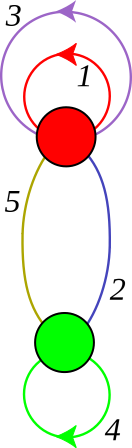
\includegraphics[width=1.0\textwidth]{PVAWMarkovSymb}\\(e)
            \end{center}\end{minipage}
\end{center}
  \caption{\label{fig:PVAdlerWeissS2HL}
(\refFig{fig:PVAdlerWeiss2HL} continued)
(c)
The sub-rectangles $\pS_j$, indicated by  the compact 5-letter alphabet
\refeq{catAlphabetPVAW2HL}.
(d)
Admissible orbits correspond to walks on the {\markGraph} for this partition.
The nodes refer to the rectangles $A$ and $B$, and the five colored links,
labeled by their lattice translation $\Ssym{j}\in\{\underline{1},0,1\}$, correspond
to the five sub-rectangles reached in one step forward-time dynamics.
(e) Compact labeling, see \refeq{catAlphabetPVAW2HL}.
}
\end{figure}
%%%%%%%%%%%%%%%%%%%%%%%%%%%%%%%%%%%%%%%%%%%%%%%%%%%%%%%%%%%%%%%


%%%%%%%%%%%%%%%%%%%%%%%%%%%%%%%%%%%%%%%%%%%%%%%%%%%%%%%%%%%%%
\begin{figure}\begin{center}
            \begin{minipage}[c]{0.30\textwidth}\begin{center}
\includegraphics[width=1.0\textwidth]{PVAdlerWeissS-c}\\(a)
            \end{center}\end{minipage}
            \hskip 2ex
            \begin{minipage}[c]{0.30\textwidth}\begin{center}
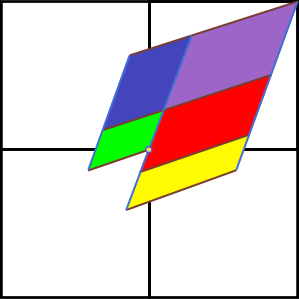
\includegraphics[width=1.0\textwidth]{PVAdlerWeissR-c}\\(b)
            \end{center}\end{minipage}
            \hskip 2ex
            \begin{minipage}[c]{0.30\textwidth}\begin{center}
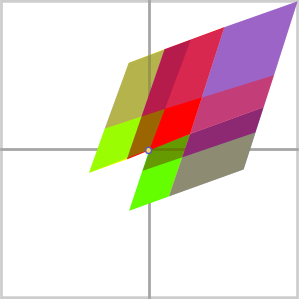
\includegraphics[width=1.0\textwidth]{PVAdlerWeissC-c}\\(c)
            \end{center}\end{minipage}
\end{center}
  \caption{\label{fig:PVAdlerWeissC}
(From \reffig{fig:PVAdlerWeiss2HL})
(a)
The forward in time sub-rectangles $\pS_j$, indicated by color / 5-letter alphabet
\refeq{catAlphabetPVAW2HL}.
(b)
The corresponding partition defined for one step backward in time (not
the partition (a) iterated back).
(c) The overlap 2-step partition. Not sure this is right.
}
\end{figure}
%%%%%%%%%%%%%%%%%%%%%%%%%%%%%%%%%%%%%%%%%%%%%%%%%%%%%%%%%%%%%%%

%%%%%%%%%%%%%%%%%%%%%%%%%%%%%%%%%%%%%%%%%%%%%%%%%%%%%
\begin{figure}
  \centering
(a)\includegraphics[width=0.2\textwidth]{HLOneStepBackwardA}
(c)\includegraphics[width=0.2\textwidth]{HLOneStepBackwardC}
(b)\includegraphics[width=0.45\textwidth]{HLOneStepBackwardB}
  \caption{\label{fig:HLOneStepBackward}
(a)
The two rectangles partition of the \PV\ cat map.
(b)
Mapped one step backward in time.
(c)
The stretched partition has been translated back to the original shape.
}
\end{figure}
%%%%%%%%%%%%%%%%%%%%%%%%%%%%%%%%%%%%%%%%%%%%%%%%%%%%%%%

\PCpost{2018-02-12}{
Can you plot the stretched domains corresponding to
\reffig{fig:PVAdlerWeiss2HL}\,(b) for one step back in time (inverse map)?
Should look something like \reffig{fig:PVAdlerWeissC}.
    }

\HLpost{2018-03-01}{
I have calculated the stretched domains corresponding to
\reffig{fig:PVAdlerWeiss2HL}\,(b) for one step back in time. The result is in
\reffig{fig:HLOneStepBackward}\,(c) which is not same as
\reffig{fig:PVAdlerWeissC}\,(b). I guess this is because I start from partition
in \reffig{fig:HLOneStepBackward}\,(a). If I start from the partition flipped
from \reffig{fig:HLOneStepBackward}\,(a) across the $\ssp_1=\ssp_0$ I will get
\reffig{fig:PVAdlerWeissC}\,(b). The overlap 2 partition is also different from
\reffig{fig:PVAdlerWeissC}\,(c). I'm not sure...
}

\PCpost{2018-03-01}{
My \reffig{fig:PVAdlerWeissC} was just a quick sloppy sketch. I'm confident that
your \reffig{fig:HLOneStepBackward} is right.
}

\HLpost{2018-02-15}
      {
I have read the section \textit{Markov Partitions for Hyperbolic Toral
Automorphisms} of Robinson's book. I'm currently working on
\refexam{exam:FP_eigs_CatMap}. The \refeq{catMapPFmat} seems not correct. I'm
working on it.
        }

\PCpost{2018-02-16}{
I'm complicating this unnecessarily - it would be nice to get the correct
5-rectangles transfer matrix \refeq{catMapPFmat}, but it is unnecessary
for our purposes: the two-rectangle partition [2$\times$2] Markov
matrix, where one sums over all admissible transitions, should suffice
(for notation, see \refeq{catAlphabetPVAW2HL} and \refref{CBmeasure}):
\beq
\left[\begin{array}{c} \phi'_A \\ \phi'_B \end{array}\right]=
L\phi=
\left[
\begin{array}{cc}
 \speriod{A{}^0\!A}+\speriod{A{}^1\!A} & \speriod{A{}^{\underline{1}}\!B} \\
 \speriod{B{}^1\!A} & \speriod{B{}^0\!B} \\
\end{array}
\right]
\left[\begin{array}{c} \phi_A \\ \phi_B \end{array}\right]
\ee{2rectTransfMatrEq}
\bea
L &=&
\left[\begin{array}{cc}
 \speriod{A{}^0\!A}+\speriod{A{}^1\!A} & \speriod{A{}^{\underline{1}}\!B} \\
 \speriod{B{}^1\!A}              & \speriod{B{}^0\!B} \\
\end{array}\right]
=
\left[\begin{array}{cc}
 \frac{|\pS_{1}|+|\pS_{3}|}{|\pS_{A}|} & \frac{|\pS_{5}|}{|\pS_{A}|} \\
 \frac{|\pS_{2}|}{|\pS_{B}|}             & \frac{|\pS_{4}|}{|\pS_{B}|} \\
\end{array}\right]
    \continue
&=&
\frac{1}{\ExpaEig}
\left[\begin{array}{cc}
 2          & \ExpaEig-2 \\
 \ExpaEig-1 & 1          \\
\end{array}\right]
\,.
\label{2rectTransfMatrEq1}
\eea
in compact notation
\(
\{A{}^0\!A, B{}^1\!A, A{}^1\!A, B{}^0\!B, A{}^{\underline{1}}\!B\}
= \{ {1}, {2}, {3}, {4}, {5}\}
\,.
\)
Then
\bea
\Det(1-zL) &=&
% \frac{1}{\ExpaEig^2}
\left|\begin{array}{cc}
 1 -2z/\ExpaEig      & -z(\ExpaEig-2)/\ExpaEig \\
 -z(\ExpaEig-1)/\ExpaEig & 1-z/\ExpaEig       \\
\end{array}\right|
    \continue
&=& 1-3\frac{z}{\ExpaEig}
     +2\frac{z^2}{\ExpaEig^2}
     -\frac{z^2}{\ExpaEig^2}(\ExpaEig-1)(\ExpaEig-2)
    \continue
&=& 1-3\frac{z}{\ExpaEig}
     -\frac{z^2}{\ExpaEig}(\ExpaEig-3)
\,,
\label{2rectDetTransfMatr}
\eea
in agreement with the loop expansion \refeq{CattyZeta1}.
    }

\begin{figure}
  \centering
\begin{minipage}[b]{0.22\textwidth}  \centering
    \includegraphics[width=1.00\textwidth]{HLPartitionSEqualTo5A}\\(a)
\end{minipage}
\begin{minipage}[b]{0.22\textwidth}  \centering
    \includegraphics[width=1.00\textwidth]{HLPartitionSEqualTo5B}\\(b)
\end{minipage}
\begin{minipage}[b]{0.22\textwidth}  \centering
    \includegraphics[width=1.00\textwidth]{HLPartitionSEqualTo5C}\\(c)
\end{minipage}
 	\caption{\label{fig:HLPartitionSEqualTo5}
(a) The 3-rectangle partition for $s=5$.
(b) The first forward iterate of the partition.
(c) I put (a) and (b) together so it obvious that the alphabet is from $-1$ to $4$.
}
\end{figure}


\PCpost{2018-02-16}{
For $s\geq 3$, the 3-letter alphabet \refeq{catAlphabetPVAW} generalizes
to
\beq
\A=\{\underline{1},0,1,\cdots,s-2\}
\,.
\ee{catAlph-s-PVAW}
What keeps the forward iterates of the small rectangle in check is the
way this area shrinks with large $\ExpaEig$ in \refeq{CatMapAreas}.
}
%Han: This curly bracket is missed so I didn't see this post until today.
%     But I guess your last post shouldn't be inside the post before?
%  Predrag:
%  sorry, meant to type \PC{2018-01-16} but wrote \PCpost{2018-01-16} instead
\HLpost{2018-02-18}{
For $s\geq3$ the alphabet for the 2- (and 3-) rectangle partition is
\refeq{catAlph-s-PVAW}: see the 3-rectangle stable and unstable manifolds
borders partition for $s=5$ in \reffig{fig:HLPartitionSEqualTo5}.
}
\PCpost{2018-02-18}{
Great.
% the figure is perfect, agrees with my hand-drawn ones. Also,
It should led to more sensible labelling of
\reffig{fig:PVAdlerWeissS2HL}\,(e) {\markGraph}, for arbitrary $s$. You
can see that, much like in the \PV\
\reffig{fig:CatMapStatesp}, there is an \emph{interior}
$(s\!-\!1)$-letter  alphabet $\Ai$ which is a full shift ($(s\!-\!1)$
loops attached to node $A$), and some kind of 2-letter \emph{exterior}
alphabet $\Ae$ that has to do with node $B$.

A well-understood alphabet can help us with solving the 2\dmn\ {\catlatt}
- there the {interior} alphabet $\Ai$ is still a full shift, while the
{exterior} alphabet $\Ae$ is a bit bigger.
}
%\PCpost{2018-02-19}{
%\refFig{fig:HLPeriodicOrbitsA}\,(i) and (j) are currently the same orbit
%$\Xx_{1 0 1 \underline{1}}=\Xx_{0 1 \underline{1}1}$ plotted
%twice; we missed (i) $\Xx_{0 0 1 1}$, \PCedit{please compute it}.
%% PC wrong again: a fatter version (?) of \reffig{fig:HLPeriodicOrbitsA}\,(a)
%}
%\HLpost{2018-02-19}{
%I have updated the orbit for $\Xx_{0 0 1 1}$ and \reffig{fig:HLPeriodicOrbitsB} (i).}

\PCpost{2018-02-19}{
The alphabet \refeq{threeLett},
\(
\Ssym{t}\in\{\underline{1},0,1\} \,
\)
is not good, as it seems not to encode any of the symmetries of
orbits in \reffigs{fig:HLPeriodicOrbitsA}{fig:HLPeriodicOrbitsB}.
    }

%%%%%%%%%%%%%%%%%%%%%%%%%%%%%%%%%%%%%%%%%%%%%%%%%%%%%%%%%%%%%
\begin{figure}
  \centering
(a)~~\includegraphics[width=0.37\textwidth]{PCLect13p9}
(b)~~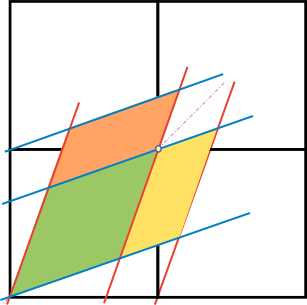
\includegraphics[width=0.37\textwidth]{PCLect13p9d}
  \caption{\label{fig:PCLect13p9d}
Abandoned attempt:
(a) The three-rectangle, time reversal symmetric generating partition for
the \PV\ cat map \refeq{PerViv:2confRepMat}, with borders given
by cat map stable-unstable manifolds.
(b)
The three-rectangle partition obtained by space reversal (reflection across the
anti-diagonal) is also a valid generating partition, but the distinct from (a).
Thus this partition does not exhibit in a simple way the space reflection
symmetry that is evident in \reffig{fig:CatMapStatesp}.
}
\end{figure}
%%%%%%%%%%%%%%%%%%%%%%%%%%%%%%%%%%%%%%%%%%%%%%%%%%%%%%%%%%%%%%%

%%%%%%%%%%%%%%%%%%%%%%%%%%%%%%%%%%%%%%%%%%%%%%%%%%%%%%%%%%%%%
\begin{figure}
  \centering
(a)~~\includegraphics[width=0.37\textwidth]{PCLect13p9}
(b)~~\includegraphics[width=0.37\textwidth]{PCLect13p9e}
  \caption{\label{fig:PCLect13p9e}
Abandoned attempt:
(a) The three-rectangle, time reversal symmetric generating partition for
the \PV\ cat map \refeq{PerViv:2confRepMat}, with borders given
by cat map stable-unstable manifolds. Large rectangle is self-dual under time
reversal (reflection across the diagonal), while the two small rectangles
are mapped into each other.
This implies that we should go to a fundamental domain (positive time only),
and recode the dynamics according to
\refexam{exam:Symm1d}~{\em $\Dn{1}$ factorization}:
% \refsect{s-C-2-fact}~{\em $\Zn{2} = \Dn{1}$ factorization}:
(b) The three-rectangle partition time reversal fundamental domain (the half of
the full partition, cut in two by the time reflection diagonal). Need to check
whether we can handle the reflection of \Ssym{n} as well.
}
\end{figure}
%%%%%%%%%%%%%%%%%%%%%%%%%%%%%%%%%%%%%%%%%%%%%%%%%%%%%%%%%%%%%%%

\PCpost{2018-02-19}{
I wonder why all cycles (except for a small kink in $\Xx_{0 1
\underline{1}1}$) turn clockwise? Reminds me of harmonic oscillator, that
also has a unique rotation direction - might be a consequence of
symplectic dynamics.
    }

\HLpost{2018-02-27}{
I have read the Chapter 15 \textit{Counting} of Chaosbook. It's not easy.
Finally have some general ideas about the \tzeta.
}

%\HLpost{2018-02-27}{
%I have tried to make the partition to be symmetric about both the
%$\ssp_1=\ssp_0$ and the $\ssp_1=-\ssp_0$, and find that it's impossible to make
%such a partition with the borders along the stable and unstable manifold.
%}


    	\HLpost{2018-01-31}{
Matrices \refeq{eigVecs} can diagonalize \refeq{PerViv:2confRepMat} (I may be wrong).
        }

\PCpost{2018-02-13}{
Your Green's function is symmetric. Diagonalize?
    }

\HLpost{2018-02-13}{
The eigenvalues of this Green's function are 1, 1/3, 1/3, 1/5. These are also
the diagonal elements of the diagonalized matrix.
    }

\PCpost{2018-02-13}{
Mhm - you sure? I was expecting $\sqrt{5}$'s. What about eigenvectors? Try
period-5. $5$ is a prime.
    }

\HLpost{2018-02-13}{
When the circulant matrix and the Green's function are [$5\!\times\!5$]
matrices, the eigenvalues of the Green's function are
\beq
1, (7+\sqrt{5})/2, (7+\sqrt{5})/2, (7-\sqrt{5})/2, (7-\sqrt{5})/2,
\ee{5cycleGreenEigs}
corresponding to eigenvectors:\\
\(
(1, 1, 1, 1, 1), \\
((-1 + \sqrt{5})/{2}, (1 - \sqrt{5})/{2}, -1, 0, 1), \\
(-1, (1 - \sqrt{5})/{2}, (-1 + \sqrt{5})/{2}, 1, 0), \\
((-1 - \sqrt{5})/{2}, (1 + \sqrt{5})/{2}, -1, 0, 1), \\
(-1, (1 + \sqrt{5})/{2}, (-1 - \sqrt{5})/{2},1, 0)
\,.
\)
    }

\PCpost{2018-02-13}{
Mhm - surprised again. I was motivated by \refeq{GreenFun00a} and
\refeq{BirVivx=b}, and expected you to (re)discover sort of a
\HREF{https://en.wikipedia.org/wiki/Circulant_matrix} {discrete Fourier
transform}, but with hyperbolic functions. Back to drawing board.
    }

\PCpost{2018-04-22}{
Fourier-transformed cycle points $\hat{\Mm}$ for the periodic points of
\reffig{fig:HLPeriodicOrbitsA}:
% PC 2018-04-22, computed with
% siminos/mathematica/DiscreteFourier.nb
%%%%%%%%%%%%%%%%%%%%%%%%%%%%%%%%%%%%%%%%%%%%%%%%%%%%%%%%%%%%
%Mma={0,0,0,1};
%Mmb={1,1,1,0};
%Mmc={0,0,1,-1};
%Mmd={0,0,-1,1};
%Mme={0,1,1,-1};
%Mmf={1,1,0,-1};
%Mmg={1,1,1,-1};
%Mmh={0,0,1,-1};
%Mmi={0,0,1,1};
%Mmj={0,1,-1,1};
\bea
\hat{\Mm}_{0 0 0 1} &=&
\frac{1}{2}
\left[1, -\ii, -1, \ii \right]
    \,\Rightarrow\quad
\hat{\ssp}=
\left[ {0}, { }, {0}, { }\right]
    \continue
\hat{\Mm}_{1 1 1            0} &=&
\frac{1}{2}
\left[3, \ii, 1, -\ii \right]
    \,\Rightarrow\quad
\hat{\ssp}=
\left[ {0}, { }, {0}, { } \right]
    \continue
\hat{\Mm}_{0 0 1 \underline{1}} &=&
\frac{1}{2}
\left[0, -1+\ii, 2, -1-\ii \right]
    \,\Rightarrow\quad
\hat{\ssp}=
\left[ {0}, { }, { }, { }\right]
    \continue
\hat{\Mm}_{0 0 \underline{1}1} &=&
\frac{1}{2}
\left[0, 1-\ii, -2, 1+\ii \right]
    \,\Rightarrow\quad
\hat{\ssp}=
\left[ {0}, { }, { }, { } \right]
    \continue
\hat{\Mm}_{0 1 1 \underline{1}} &=&
\frac{1}{2}
\left[1, -1+2 \ii, 1, -1-2\ii \right]
    \,\Rightarrow\quad
\hat{\ssp}=
\left[ {0}, { }, { }, { } \right]
    \continue
\hat{\Mm}_{1 1 0 \underline{1}} &=&
\frac{1}{2}
\left[1, 1+2 \ii, 1, 1-2\ii \right]
    \,\Rightarrow\quad
\hat{\ssp}=
\left[ {0}, { }, { }, { } \right]
    \continue
\hat{\Mm}_{1 1 1 \underline{1}} &=&
\frac{1}{2}
\left[2, 2\ii, 2, -2\ii \right]
    \,\Rightarrow\quad
\hat{\ssp}=
\left[ { }, { }, { }, { } \right]
    \continue
\hat{\Mm}_{0 0 1 \underline{1}} &=&
\frac{1}{2}
\left[0, -1+\ii, 2, -1-\ii \right]
    \,\Rightarrow\quad
\hat{\ssp}=
\left[ { }, { }, { }, { } \right]
    \continue
\hat{\Mm}_{0 0 1 1} &=&
\frac{1}{2}
\left[2, -1-\ii, 0, -1+\ii \right]
    \,\Rightarrow\quad
\hat{\ssp}=
\left[ {0}, { }, { }, { } \right]
    \continue
\hat{\Mm}_{0 1 \underline{1}1} &=&
\frac{1}{2}
\left[1,1,-3,1 \right]
    \,\Rightarrow\quad
\hat{\ssp}=
\left[ {0}, { }, { }, { } \right]
    \ceq
\label{FourierPointsCorner}
\eea
Each cycle has 3 further cycle points, not computed here (but that should be
plotted in the Brilliuon zone).
I did not compute $\hat{\ssp}_k$,
as that is a trivial multiplication by the diagonalized Green's function
\refeq{FourierSpacePoints2}.

Take home messages; writing Fourier transforms of periodic points
analytically is not useful. Only cycle-4 orbits are related to Gaussian
integers, for other orbits there will be no nice analytic formulas. And
already for 4-cycles, the phases are not rational fractions of $2\pi$.
For example for $1+2\ii$ the polar form phase in radians is $\arctan 2 =
1.10715$.
}

\PCpost{2018-02-21}{
The Green's function \refeq{HLGreensfunc} and eigenvalues and eigenvectors
\refeq{5cycleGreenEigs} all have Toeplitz matrix structure. In case like this,
when the problem has been around for centuries, reading literature is a great
time saver, especially if someone has already done the dive into literature for
you. You can understand your Mathematica results by the analytic solution for
any cycle lengts and any $s$, for example \refeq{3diagToepEigs} and
\refeq{HuCon95Helmh}. Here you learn, explicitly, that for $s>2$, the lattice
should not be expanded in Fourier modes, but in $\sinh$ and $\cosh$'s. There are
some other cute formulas in literatures, for example \refeq{BirVivx=b} and
\refeq{BirViv(3.5)}.
    }

\PCpost{2018-04-25}{
Reciprocal lattice is standard. I think you need to use stable / unstable
eigenvectors in configuration space, compute reciprocal lattice with respect
to them. Will continue writeup (unless you beat me to it:)
}

\PCpost{2018-04-25}{
Scratch stable / unstable
eigenvectors - there is no integer-multiple tiling along those directions (I guess
it is a antiperiodic tiling), the only configuration space vector is 1\dmn,
pointing for \PV\ cat map along the vertical direction.
}

\PCpost{2018-04-22}{
Trying to get some feeling for the Fourier space representation, by
computing the rhomboid corner partition 4-cycles
\refeq{FourierPointsCorner}, to see how they differ from the rhomboid
center partition 4-cycles \refeq{FourierSpacePoints}. The main take home
message; analytic form of these Fourier transforms does not seem helpful,
seems best to plot them numerically, in complex plane for the reciprocal
lattice / Brilluion zone (not attempted yet).
}

\HLpost{2018-04-25}{
I plotted all of the admissible 11-cycles of the rhomboid corner partition in
complex plane in \reffig{fig:HL11CyclRecipLatt}. It looks like if I plot
the figure with $k$ from -5 to 5 instead of from 0 to 10 (which is to move
the part with $k>5$ to the left side of the origin), this figure will be
symmetric about $k=0$ plane. I tried to make some changes to the figure but
the program keep getting frozen when I plot the figure. I will try again
later on a desktop.
}

%%%%%%%%%%%%%%%%%%%%%%%%%%%%%%%%%%%%%%%%%%%%%%%%%%%%%%%
\begin{figure}
  \centering
\includegraphics[width=0.6\textwidth]{HL11-cyclesReciprocalLattice}
  \caption{\label{fig:HL11CyclRecipLatt}
The Fourier transform of the 39601 period $\cl{}=11$ {\lattstate}s
(see \refeq{catMapN_n-s=3}) of the
rhomboid corner partition in the complex plane.
}
\end{figure}
%%%%%%%%%%%%%%%%%%%%%%%%%%%%%%%%%%%%%%%%%%%%%%%%%%%%%%%

\PCpost{2018-04-25}{
Fascinating. Is it possible to generate a version that is 3D live (can be rotated)?
Also, we need to plot these in the Brilliuon zone, not just raw Fourier...
}

\end{description}

\section{Rhomboid center partition}
\label{sect:RhombCenter}

A generating partition must map borders onto borders under dynamics
(\AW),
but a really nice partition should also embody all
symmetries of the dynamics; invariance under spatial reflections and the
time reversal.

For the \PV\ cat map the  dynamics commutes with the spatial
reflection $\Refl$ (across anti-diagonal), while time reversal will
require extra thinking.

For the \PV\ cat map the flip across the $\ssp_1=\ssp_0$
diagonal together with the reversal of the direction of evolution is the
\Dn{1} symmetry that corresponds to the invariance of cat map under time
reversal.


\begin{description}

\PCpost{2018-04-20}{{\color{red}
Currently \reffig{fig:HLStretchedPartition}\,(b) does not map a border
onto a border within region D of
\reffig{fig:HL7-rectanglePartition}\,(a); sadly, the partition studied in
this section is not generating.
                    }}

\PCpost{2018-02-18}{
\PV\ alphabet can be made symmetric under spatial reflection
by picking the origin in the middle of the unit interval, see
\refsect{sect:catAdlerWeiss}.
The tiling \reffig{fig:PCLect13p12}\,(b) and the partition
\reffig{fig:PCLect13p9a}\,(b) suggests that partition should
be centered differently to fully exploit the symmetries of the tiling -
perhaps with the fixed point in the center of the square, rather with the
fixed point in the corner.
}

\PCpost{2018-02-28}{
A proposal for a space and time symmetric partition in
\reffig{fig:PCLect13p13a}. Do you see how to fix it?
    }

%%%%%%%%%%%%%%%%%%%%%%%%%%%%%%%%%%%%%%%%%%%%%%%%%%%%%%%%%%%%%
\begin{figure}
  \centering
(a)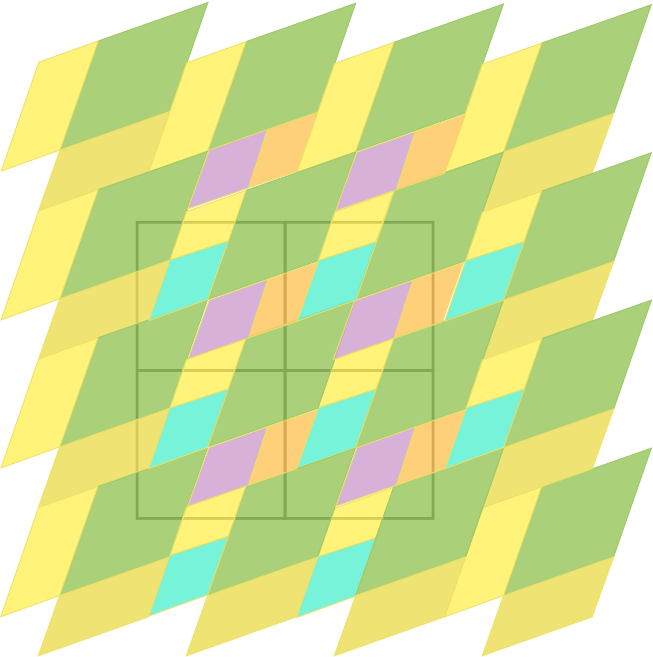
\includegraphics[width=0.45\textwidth]{PCLect13p13a}
(b)\includegraphics[width=0.45\textwidth]{PCLect13p13b}
  \caption{\label{fig:PCLect13p13a}
Abandoned attempt:
(a)
Tiling of the square lattice by a five-rectangle, time reversal and space
reflection symmetric partition. Note that we have used the continuous
translation invariance to place the center of the large tile $A$ at the origin.
(b)
An almost a generating five-rectangle, time reversal and space reflection
symmetric partition, except that the yellow / orange rectangles appear twice,
so the area this covers exceeds the unit area.
}
\end{figure}
%%%%%%%%%%%%%%%%%%%%%%%%%%%%%%%%%%%%%%%%%%%%%%%%%%%%%%%%%%%%%%%

\HLpost{2018-02-28, 018-03-18}{
Yes! A space reflection symmetric partition in \reffig{fig:PCLect13p13a}
is obtained by cutting the yellow and orange rectangles into halves, as
shown in \reffig{fig:HLSymmetricPartition}. That is natural in the
centered unit square tiling of the plane, \ie, the grid going through
multiples of $(1/2,1/2)$.
\refFig{fig:HLSymmetricPartition}\,(c) shows that this partition
tiles the whole space.
The forward image of the partition of \reffig{fig:HLSymmetricPartition}\,(b)
\reffig{fig:HLStretchedPartition}. \refFig{fig:HLStretchedPartition} is the
labeled 7-rectangle partition, together with the \markGraph.
The alphabet is
\beq
\Ssym{t}\in\{\underline{2},\underline{1},0,1,2\}
\,.
\ee{fiveLett}
}



%%%%%%%%%%%%%%%%%%%%%%%%%%%%%%%%%%%%%%%%%%%%%%%%%%%%%%%
\begin{figure}
  \centering
(a)\includegraphics[width=0.35\textwidth]{HLSymmetricPartitionA}
(b)\includegraphics[width=0.35\textwidth]{HLSymmetricPartitionB}
(c)\includegraphics[width=0.5\textwidth]{HLSymmetricPartitionC}
  \caption{\label{fig:HLSymmetricPartition}
(a)
Start with the partition of \reffig{fig:PCLect13p13a}\,(b).
The dashed lines in the directions of stable and unstable manifolds cut
the yellow and orange rectangles into halves.
(b)
The symmetric partition obtained by removing halves of yellow and orange
rectangles has area $1$.
(c)
The partition tiles the square lattice.
}
\end{figure}
%%%%%%%%%%%%%%%%%%%%%%%%%%%%%%%%%%%%%%%%%%%%%%%%%%%%%%%

%\PCpost{2018-02-28}{
%\refFig{fig:HLSymmetricPartition} did not work for me. The area is now unit
%area, but the 1/2's you throw away are now holes in the tiling, I believe.
%}
%
%\HLpost{2018-03-01}{
%I believe there is no hole in the tiling when we throw away the 1/2's. I add
%\reffig{fig:HLSymmetricPartition}\,(c) so you can see the new partition can
%perfectly cover the whole area.
%}

%%%%%%%%%%%%%%%%%%%%%%%%%%%%%%%%%%%%%%%%%%%%%%%%%%
\begin{figure}
  \centering
\begin{minipage}[b]{0.22\textwidth}  \centering
    \includegraphics[width=1.00\textwidth]{HLStretchedPartition1}\\(a)
\end{minipage}
\begin{minipage}[b]{0.30\textwidth}  \centering
    \includegraphics[width=1.00\textwidth]{HLStretchedPartition2}\\(b)
\end{minipage}
\begin{minipage}[b]{0.40\textwidth}  \centering
    \includegraphics[width=1.00\textwidth]{HLStretchedPartition3}\\(c)
\end{minipage}
 	\caption{\label{fig:HLStretchedPartition}
(a) The forward image of the 7-rectangle partition
    \reffig{fig:HLSymmetricPartition}\,(b).
(b) The stretched partition overlaid over the original partition.
(c) The stretched partition overlaid over the tiled lattice.
The $x$ and $y$ axes are not plotted to the same scale.
}
\end{figure}
%%%%%%%%%%%%%%%%%%%%%%%%%%%%%%%%%%%%%%%%%%%%%%%%%

\PCpost{2018-03-18}{
Staring at the partition of \reffig{fig:HLStretchedPartition}: no wander
I failed to draw it by hand. In
\reffig{fig:HLStretchedPartition}\,(b) there are little holes next to $D$ and $G$
and the weird overlaps $\pS_D\cap f(\pS_E)$, $\pS_G\cap f(\pS_F)$,
it's a miracle that the partition works. You might want to check it for
longer period orbits in $\pS_D$.
}

%%%%%%%%%%%%%%%%%%%%%%%%%%%%%%%%%%%%%%%%%%%%%%%%%%%%%%%%%%%%%
\begin{figure}
  \centering
(a)\includegraphics[width=0.4\textwidth]{HL7-rectanglePartition}
(b)\includegraphics[width=0.5\textwidth]{HLTransitionGraph}
  \caption{\label{fig:HL7-rectanglePartition}
(a) The labeled 7-rectangle partition, and
(b) the corresponding 7-node {\markGraph}.
}
\end{figure}
%%%%%%%%%%%%%%%%%%%%%%%%%%%%%%%%%%%%%%%%%%%%%%%%%%%%%%%%%%%%%%%

%\PCpost{2018-03-01}{
%Wow! Persuasive. And pretty.
%I did not like cutting into 1/2's, because that seems unnatural to me
%from the dynamical point of view.
%I though we would have to overcount
%yellow / oranges, and then divide them out in zeta functions, like
%one does for the overcounted fixed point at the the green / blue / purple
%corner (is it still there?).
%}

\HLpost{2018-03-05}{
All period 4 {\orbit}s in the symmetric partition
\reffig{fig:HLSymmetricPartition}\,(b) are
\bea
\Xx_{1 1 \underline{1} \underline{1}} &=& \frac{1}{15}
\left[
\begin{array}{cccc}
 {5} &
 {5} &
 {-5} &
 {-5}
\end{array}
\right]
    \,,\qquad
\Xx_{0 \underline{2} 0 2}= \frac{1}{15}
\left[
\begin{array}{cccc}
 {0} &
 {-10} &
 {0} &
 {10}
\end{array}
\right]
    \continue
\Xx_{0 0 1 \underline{1}} &=& \frac{1}{15}
\left[
\begin{array}{cccc}
 {-1} &
 {1} &
 {4} &
 {-4}
\end{array}
\right]
    \,,\qquad
\Xx_{0 0 \underline{1} 1}= \frac{1}{15}
\left[
\begin{array}{cccc}
 {1} &
 {-1} &
 {-4} &
 {4}
\end{array}
\right]
    \continue
\Xx_{1 \underline{2} 2 \underline{1}} &=& \frac{1}{15}
\left[
\begin{array}{cccc}
 {2} &
 {-7} &
 {7} &
 {-2}
\end{array}
\right]
    \,,\qquad
\Xx_{2 \underline{2} 1 \underline{1}}= \frac{1}{15}
\left[
\begin{array}{cccc}
 {7} &
 {-7} &
 {2} &
 {-2}
\end{array}
\right]
    \continue
\Xx_{0 1 \underline{1} 1} &=& \frac{1}{15}
\left[
\begin{array}{cccc}
 {4} &
 {6} &
 {-1} &
 {6}
\end{array}
\right]
    \,,\qquad
\Xx_{\underline{1} 0 \underline{1} 1}= \frac{1}{15}
\left[
\begin{array}{cccc}
 {-6} &
 {-4} &
 {-6} &
 {1}
\end{array}
\right]
    \continue
\Xx_{1 0 1 \underline{2}} &=& \frac{1}{15}
\left[
\begin{array}{cccc}
 {3} &
 {2} &
 {3} &
 {-8}
\end{array}
\right]
\,,\qquad
\Xx_{\underline{1} 0 \underline{1} 2}= \frac{1}{15}
\left[
\begin{array}{cccc}
 {-3} &
 {-2} &
 {-3} &
 {8}
\end{array}
\right]
    \ceq
\label{4cyclesPoints}
\eea
The orbits are in
\reffigs{fig:HLSymmetric4CyclesA}{fig:HLSymmetric4CyclesB}. All
orbits are symmetric about both $\ssp_1=\ssp_0$ and $\ssp_1=-\ssp_0$,
either self-dual or come in pairs.
}

\PCpost{2018-03-05}{
Beautiful! We have the doubly symmetric partition nailed. I do not think
this is anywhere in the literature. Can you connect to symmetries to
cycle itineraries?
    }

\HLpost{2018-04-08}{
I have recomputed the 4-cycles of \refeq{4cyclesPoints} in the
face-centered \PV\ unit square non-partition.  That screws up
the above
$\Xx_{1 0 1 \underline{2}}$,
$\Xx_{0 \underline{2} 0 2}$,
and
$\Xx_{\underline{1} 0 \underline{1} 2}$:
\bea
\Xx_{\underline{1} \underline{1} 1 1} &=& \frac{1}{15}
\left[
\begin{array}{cccc}
 {-5} &
 {-5} &
 {5} &
 {5}
\end{array}
\right]
    \,,\qquad
\HLedit{
\Xx_{\underline{1} 0 1 0}
        } = \frac{1}{15}
\left[
\begin{array}{cccc}
 {-5} &
 {0} &
 {5} &
 {0}
\end{array}
\right]
    \continue
\Xx_{0 0 1 \underline{1}} &=& \frac{1}{15}
\left[
\begin{array}{cccc}
 {-1} &
 {1} &
 {4} &
 {-4}
\end{array}
\right]
    \,,\qquad
\Xx_{0 0 \underline{1} 1}= \frac{1}{15}
\left[
\begin{array}{cccc}
 {1} &
 {-1} &
 {-4} &
 {4}
\end{array}
\right]
    \continue
\Xx_{1 \underline{2} 2 \underline{1}} &=& \frac{1}{15}
\left[
\begin{array}{cccc}
 {2} &
 {-7} &
 {7} &
 {-2}
\end{array}
\right]
    \,,\qquad
\Xx_{2 \underline{2} 1 \underline{1}}= \frac{1}{15}
\left[
\begin{array}{cccc}
 {7} &
 {-7} &
 {2} &
 {-2}
\end{array}
\right]
    \continue
\Xx_{0 1 \underline{1} 1} &=& \frac{1}{15}
\left[
\begin{array}{cccc}
 {4} &
 {6} &
 {-1} &
 {6}
\end{array}
\right]
    \,,\qquad
\Xx_{\underline{1} 0 \underline{1} 1}= \frac{1}{15}
\left[
\begin{array}{cccc}
 {-6} &
 {-4} &
 {-6} &
 {1}
\end{array}
\right]
    \continue
\HLedit{
\Xx_{0 0 0 1}
        } &=& \frac{1}{15}
\left[
\begin{array}{cccc}
 {3} &
 {2} &
 {3} &
 {7}
\end{array}
\right]
\,,\qquad
\HLedit{
\Xx_{\underline{1} 0 0 0}
       } = \frac{1}{15}
\left[
\begin{array}{cccc}
 {-7} &
 {-3} &
 {-2} &
 {-3}
\end{array}
\right]
\nnu\\
\label{4cyclesPointsB}
\eea
    }

%\HLpost{2018-03-12}{
%Predrag's relabelling of \reffig{fig:HLSymmetric4CyclesA}\,(a) was wrong. The
%correct label is $\Xx_{1 1 \underline{1} \underline{1}}$ (as fixed in the
%figure).
%}

%%%%%%%%%%%%%%%%%%%%%%%%%%%%%%%%%%%%%%%%%%%%%%%
\begin{figure}
  \centering
(a) \includegraphics[width=0.40\textwidth]{HLSymmetric4Cycles1}
\hskip 1ex
(b) \includegraphics[width=0.40\textwidth]{HLSymmetric4Cycles2}
\\
(c)  \includegraphics[width=0.40\textwidth]{HLSymmetric4Cycles3}
\hskip 1ex
(d)  \includegraphics[width=0.40\textwidth]{HLSymmetric4Cycles4}
\\
(e) \includegraphics[width=0.40\textwidth]{HLSymmetric4Cycles7}
\hskip 1ex
(f) \includegraphics[width=0.40\textwidth]{HLSymmetric4Cycles8}
 	\caption{\label{fig:HLSymmetric4CyclesA}
All 4-cycles from \refeq{4cyclesPoints}:
(a)
% HL corrected 2017-03-12 $\Xx_{0 1 0 \underline{1}}$
% (presumably Predrag's relabelling is wrong, the correct one is
$\Xx_{1 1 \underline{1} \underline{1}}$
% the first one in \refeq{4cyclesPoints}),
(b) $\Xx_{0 \underline{2} 0 2}$,
(c) $\Xx_{0 0 1 \underline{1}}$,
(d) $\Xx_{0 0 \underline{1}1}$,
(e) $\Xx_{\underline{1} 1 \underline{2} 2}$,
(f) $\Xx_{2 \underline{2} 1 \underline{1}}$,
(g) to (j) continued in \reffig{fig:HLSymmetric4CyclesB}.
    }
\end{figure}

%%%%%%%%%%%%%%%%%%%%%%%%%%%%%%%%%%%%%%%%%%%%%%%
\begin{figure}
  \centering
(a) \includegraphics[width=0.40\textwidth]{HL4Cycle-1-111}
\hskip 1ex
(b) \includegraphics[width=0.40\textwidth]{HL4Cycle-1010}
\\
(c)  \includegraphics[width=0.40\textwidth]{HL4Cycle-1001}
\hskip 1ex
(d)  \includegraphics[width=0.40\textwidth]{HL4Cycle-1100}
\\
(e) \includegraphics[width=0.40\textwidth]{HL4Cycle-22-11}
\hskip 1ex
(f) \includegraphics[width=0.40\textwidth]{HL4Cycle-21-12}
 	\caption{\label{fig:HLsquareFaceCentered4CyclesA}
All 4-cycles from \refeq{4cyclesPoints} plotted in ``Lagrangian'' coordinates
$\{\ssp_{t-1},\, \ssp_{t+1}\}$, in the order of
\reffig{fig:HLSymmetric4CyclesA}. The 7-rectangle partition
\reffig{fig:HLSymmetricPartition}\,(b), appropriate to $\{\ssp_{t},\,
\ssp_{t+1}\}$ plots, is included only to guide the eye.
(a)
$\Xx_{\underline{1} \underline{1} 1 1}$ is
a ``Laplacian'' self-retracing 2-cycle \refeq{LaplacianSelfDual11-1-1}.
(b)
$\Xx_{0 \underline{2} 0 2}$
% $\Xx_{\underline{1} 0 1 0}$, once replotted as
is a ``Laplacian'' self-retracing 2-cycle \refeq{LaplacianSelfDual1-202}.
(c) $\Xx_{0 0 1 \underline{1}}$  and its time reversal
(d) $\Xx_{0 0 \underline{1}1}$   map into one cycle;
(e) $\Xx_{1 \underline{2} 2 \underline{1}}$
    and its time reversal
(f) $\Xx_{2 \underline{2} 1 \underline{1}}$ map into one cycle;
(g) to (j) continued in \reffig{fig:HLsquareFaceCentered4CyclesB}.
    }
\end{figure}
%%%%%%%%%%%%%%%%%%%%%%%%%%%%%%%%%%%%%%%%%%%%%%%

\begin{figure}
  \centering
(g)  \includegraphics[width=0.40\textwidth]{HLSymmetric4Cycles9}
\hskip 1ex
(h)  \includegraphics[width=0.40\textwidth]{HLSymmetric4Cycles10}
\\
(i)  \includegraphics[width=0.40\textwidth]{HLSymmetric4Cycles5}
\hskip 1ex
(j)  \includegraphics[width=0.40\textwidth]{HLSymmetric4Cycles6}
 	\caption{\label{fig:HLSymmetric4CyclesB}
Continuation of \reffig{fig:HLSymmetric4CyclesA}:
(g) $\Xx_{1 0 1 \underline{2}}$,
(h) $\Xx_{\underline{1} 0 \underline{1} 2}$
(i) $\Xx_{0 1 \underline{1} 1}$,
and
(j) $\Xx_{0 \underline{1} 1 \underline{1}}$,
}
\end{figure}
%%%%%%%%%%%%%%%%%%%%%%%%%%%%%%%%%%%%%%%%%%%%%%%

%%%%%%%%%%%%%%%%%%%%%%%%%%%%%%%%%%%%%%%%%%%%%%%
\begin{figure}
  \centering
(g)  \includegraphics[width=0.40\textwidth]{HL4Cycle-1101}
\hskip 1ex
(h)  \includegraphics[width=0.40\textwidth]{HL4Cycle-10-11}
\\
(i)  \includegraphics[width=0.40\textwidth]{HL4Cycle0001}
\hskip 1ex
(j)  \includegraphics[width=0.40\textwidth]{HL4Cycle-1000}
 	\caption{\label{fig:HLsquareFaceCentered4CyclesB}
Continuation of \reffig{fig:HLsquareFaceCentered4CyclesA} -
the space reflection dual pairs:
(g) $\Xx_{0 1 \underline{1} 1}$  and its time reversal
(h) $\Xx_{\underline{1} 0 \underline{1} 1}$  map into
space-reflection dual 4-cycles;
(i) $\Xx_{1 0 1 \underline{2}}$
and
(j) $\Xx_{\underline{1} 0 \underline{1} 2}$ map into
space-reflection dual 4-cycles.
}
\end{figure}
%%%%%%%%%%%%%%%%%%%%%%%%%%%%%%%%%%%%%%%%%%%%%%%

%\PCpost{2018-02-12}{
%I do think you want to plot all periodic points by small dots (with a
%different color for each cycle) in the partition of
%\reffig{fig:PVAdlerWeiss2HL}\,(c). You will like the result:)
%    }

\PCpost{2018-03-05}{
I still think that if one day you plot all cycle {\em points} (no lines
connecting them) on a single copy of the generating partition, you'll find the
resulting picture very cute:)

A hint from literature: Percival and Vivaldi\rf{PerViv} write:
``For the cat maps the periodic orbits lie on a rational lattice, so all surds
cancel, as shown in the companion paper\rf{PerViv87b} on the number theory of
the periodic orbits of the automorphisms of the torus.''

\refSect{sect:NoPOs}~{\em Numbers of periodic orbits} and
\refsect{sect:AKS1stApp}~{\em \Po s - first approach} might also help
with developing some intuition about \reffig{fig:HLAllCyclePoints}.
}

\PCpost{2018-03-07}{
The alphabet \refeq{fiveLett} seems to make sense.
Space reflection acts as
\beq
j \leftrightarrow \underline{j}
\,.
\ee{spaceReflSymb}
The total translation (the sum of symbols) is zero
(the orbit is periodic, standing) for all, except for
\reffig{fig:HLSymmetric4CyclesB}\,(i) and (j) which translate by $\pm 1$
(the orbit is relative periodic, running).
%and (a) $\Xx_{0 0 \underline{1} \underline{1}}$
%which looks wrong (I have now changed it to $\Xx_{0 \underline{1} 0 1}$,
%presumably my relabelling is wrong, the correct one is
%$\Xx_{1 1 \underline{1} \underline{1}}$,
%the first one in \refeq{4cyclesPoints})).

The time reversal should reverse the order of symbols, which it seems to
do, at least for \reffigs{fig:HLSymmetric4CyclesA}
{fig:HLSymmetric4CyclesB}:
\beq
(c,d)\; {0 0 1 \underline{1}}
    \leftrightarrow
        {0 0 \underline{1}1}
    \,,\quad
(e,f)\; {\underline{1} 1 \underline{2} 2}
    \leftrightarrow
   {2 \underline{2} 1 \underline{1}}
\,,
\ee{spaceReflSymb}
rest self-dual.
}

\HLpost{2018-03-15}{
In \reffig{fig:HLAllCyclePoints} I plotted all the cycle points on a single
copy of the partition for both partitions of
\reffigs{fig:PVAdlerWeiss2HL}{fig:HLSymmetricPartition}.
}

%%%%%%%%%%%%%%%%%%%%%%%%%%%%%%%%%%%%%%%%%%%%%%%%%%%%%%%%%%%%%
\begin{figure}
  \centering
(a)\includegraphics[width=0.40\textwidth]{HLAllCyclePointsB}
(b)\includegraphics[width=0.40\textwidth]{HLAllCyclePointsA}
  \caption{\label{fig:HLAllCyclePoints}
All period 4 {\orbit}s in the partition of
(a) \reffig{fig:PVAdlerWeiss2HL},
and
(b) \reffig{fig:HLSymmetricPartition}.
The holes correspond to missing cycle-1 and cycle-2 points.
        }
\end{figure}
%%%%%%%%%%%%%%%%%%%%%%%%%%%%%%%%%%%%%%%%%%%%%%%%%%%%%%%%%%%%%%%

%%%%%%%%%%%%%%%%%%%%%%%%%%%%%%%%%%%%%%%%%%%%%%%%%%%%%%%%%%%%%
\begin{figure}
  \centering
(a) \includegraphics[width=0.40\textwidth]{HLAllCyclePointsC}
(b) \includegraphics[width=0.40\textwidth]{HLAllCyclePointsD}
% former \label{fig:HLAllCyclePoints3}
  \caption{\label{fig:HLAllCyclePoints2}
(a) All periodic points that belong to the 1 ({\color{purple}purple}), 2
({\color{blue}blue}) and 4 ({\color{red}red}) {\orbit}s,
plotted in ``Hamiltonian'' coordinates
$\{\ssp_{t},\, \ssp_{t+1}\}$.
The period 1- and 2-{\orbit}s fill the holes between
period 4 {\orbit}s in the
\reffig{fig:HLAllCyclePoints}\,(b). The 3 ({\color{green}green})
{\orbit}s start a new grid, to be filled out by the period 6, 9, etc
{\orbit}s.
(b) All periodic points that belong to the period 4 {\orbit}s of
\reffig{fig:HLAllCyclePoints2} plotted in ``Lagrangian'' coordinates
$\{\ssp_{t-1},\, \ssp_{t+1}\}$. The 7-rectangle partition
\reffig{fig:HLSymmetricPartition}\,(b), appropriate to $\{\ssp_{t},\,
\ssp_{t+1}\}$ plots, is included only to guide the eye.
% but modulo face centered unit square,
% rather than the ``symmetric'' partition indicated in (a).
The numbers of {\orbit}s are listed in \refeq{noPrimeCycs=3a}.
        }
\end{figure}
%%%%%%%%%%%%%%%%%%%%%%%%%%%%%%%%%%%%%%%%%%%%%%%%%%%%%%%%%%%%%%%

\HLpost{2018-03-22}{
I have added the period 1, 2 and 3 {\orbit}s to
\reffig{fig:HLAllCyclePoints2}. The period 1 and 2 {\orbit}s fill the
holes of \reffig{fig:HLAllCyclePoints}\,(b). Each of the period 3
{\orbit}s has only one symmetry, and they have the other symmetry in
pairs.
}

\PCpost{2018-03-13}{
An aside, \PCedit{not even right, a failed attempt kept here only for the record}:
going from the partition of
\reffig{fig:PVAdlerWeiss2HL} to the partition of
\reffig{fig:HLSymmetricPartition} we have translated the origin to
$\hat{\ssp}_t= \ssp_t - 1/2$, so the map \refeq{PerViv:2confRepMat} is now
\beq
\left[\begin{array}{c}
 \hat{\ssp}_{t+1}'  \\
 \hat{\ssp}_{t}'
 \end{array} \right]
 =
{\bf A}
\left[\begin{array}{c}
 \hat{\ssp}_{t}  \\
 \hat{\ssp}_{t-1}
 \end{array} \right]
 -  \frac{1}{2}
 \left[\begin{array}{c}
 0  \\
 s-2
 \end{array} \right]
\,.
\ee{PVmapCentered}
I'm not sure why we would be allowed to drop such translational terms. A cute
fact is that Percival and Vivaldi\rf{PerViv} actually define the map
\refeq{PerViv:2confRepMat} on $\ssp_t \in [-1/2,1/2]$ interval, \ie, without
the translation term in \refeq{PVmapCentered}. Such translations should not
affect the map (it's the same automorphism of the torus, just in different
coordinates) but I do not have a clean argument that they do not matter.
    }

\HLpost{2018-03-15}{
We didn't change the origin when the partition changed from
\reffig{fig:PVAdlerWeiss2HL} to \reffig{fig:HLSymmetricPartition}. The
map is also not changed. What we did is changing the boundary of the
partition. So the map is still:
\beq
\left[\begin{array}{c}
\ssp_{t+1}  \\
\ssp_{t}
 \end{array} \right]
 =
{\bf A}
\left[\begin{array}{c}
\ssp_{t}  \\
\ssp_{t-1}
 \end{array} \right]
\,.
\ee{HLmapCentered}
}

\PCpost{2018-04-20}{{\color{red}
Currently \reffig{fig:HLStretchedPartition}\,(b) does not map a border
onto a border within region D of
\reffig{fig:HL7-rectanglePartition}\,(a); it looks as though D would have
to be cut horizontally into two halves, and even that does not complete
the task. So, sadly, the partition studied in this section is not
generating, and (for time being?) we have to give up on the whole section.
                    }}
\end{description}

\subsection{Reduction to the reciprocal lattice}
\label{sect:RhombCenterFT}
\begin{description}
\PCpost{2018-03-18}{
Check in $d=1$ whether \refeq{FourieTrField} together with the inverse
Fourier transform \refeq{inFouriTransf} recovers any of your \po s?

Does the circulant eigenvalue formula \refeq{circMatr} explain your
\refeq{5cycleGreenEigs}?
    }

\PCpost{2018-03-19}{
Does the inverse Fourier transform of the propagator in
\refeq{FourieTrField} reproduce the usual $d=1$ configuration
Green's function \refeq{GreenFun00b}?
}

\HLpost{2018-03-22}{
In $d = 1$, \refeq{FourieTrField} can recover the periodic orbits.
\refeq{FourieTrField} can be written as:
\beq
\hat{\textbf{\ssp}}
= \operatorname{diag}(\lambda)^{-1}\,\hat{\textbf{\Ssym{}}}
\,,
\ee{HLFourieTrField}
where $\lambda$ is the eigenvalue of the damped Poisson matrix
\refeq{LinearConnSum}. Then we have:
\beq
\textbf{\ssp}
= U^{\dagger}\operatorname{diag}(\lambda)^{-1}U\,\textbf{\Ssym{}}
\,,
\ee{HLFourieTrField1}
When $d=1$, $s=3$ and $n=4$ (4-cycles),
\beq
 \operatorname{diag}(\lambda)^{-1}=
 \left(
\begin{array}{cccc}
 1 & 0 & 0 & 0 \\
 0 & 3 & 0 & 0 \\
 0 & 0 & 5 & 0 \\
 0 & 0 & 0 & 3 \\
\end{array}
\right)
\ee{HLDiagonalMatrix}
Then the Green's function for 4-cycle is:
\beq
\gd = U^{\dagger}\operatorname{diag}(\lambda)^{-1}U=
\frac{1}{15}
\left(
\begin{array}{cccc}
 7 & 3 & 2 & 3 \\
 3 & 7 & 3 & 2 \\
 2 & 3 & 7 & 3 \\
 3 & 2 & 3 & 7 \\
\end{array}
\right)
\ee{HLGreensFunction1dn=4}
which is same as \refeq{HLGreensfunc}.

Using \refeq{circMatr} we can also get the result of \refeq{5cycleGreenEigs}.
% Also I think there is a typo in \refeq{3diagCircEigs}.
% PC, thanks - now fixed as you suggested.
}

\PCpost{2018-04-18}{
Can you plot the Fourier space \refeq{FourieTrField} points
$\hat{\ssp}_k,\,\hat{\Ssym{}}_k$ corresponding to
your \po s of \reffig{fig:HLAllCyclePoints2}\,(a)?
Interpret what you get?
    }

\HLpost{2018-04-18}{
$\hat{\ssp}_k,\,\hat{\Ssym{}}_k$ for the periodic points of
\reffig{fig:HLAllCyclePoints2}\,(a):
\bea
\hat{\Mm}_{1 1 \underline{1} \underline{1}} =
\left[
\begin{array}{cccc}
 {0} &
 {\sqrt{2}\,e^{\ii \pi/4}} &
 {0} &
 {\sqrt{2}\,e^{-\ii \pi/4}}
\end{array}
\right]
    \,&\Rightarrow&\quad
\hat{\Xx}=
\left[
\begin{array}{cccc}
 {0} &
 {\frac{\sqrt{2}\,e^{\ii \pi/4}}{3}} &
 {0} &
 {\frac{\sqrt{2}\,e^{-\ii \pi/4}}{3}}
\end{array}
\right]
    \continue
\hat{\Mm}_{0 \underline{2} 0 2} =
\left[
\begin{array}{cccc}
 {0} &
 {-2\,e^{\ii \pi/2}} &
 {0} &
 {-2\,e^{-\ii \pi/2}}
\end{array}
\right]
    \,&\Rightarrow&\quad
\hat{\Xx}=
\left[
\begin{array}{cccc}
 {0} &
 {-\frac{2}{3}\,e^{\ii \pi/2}} &
 {0} &
 {-\frac{2}{3}\,e^{-\ii \pi/2}}
\end{array}
\right]
    \continue
\hat{\Mm}_{0 0 1 \underline{1}} =
\left[
\begin{array}{cccc}
 {0} &
 {-\frac{e^{-\ii \pi/4}}{\sqrt{2}}} &
 {1} &
 {-\frac{e^{\ii \pi/4}}{\sqrt{2}}}
\end{array}
\right]
    \,&\Rightarrow&\quad
\hat{\Xx}=
\left[
\begin{array}{cccc}
 {0} &
 {-\frac{e^{-\ii \pi/4}}{3\sqrt{2}}} &
 {\frac{1}{5}} &
 {-\frac{e^{\ii \pi/4}}{3\sqrt{2}}}
\end{array}
\right]
    \continue
\hat{\Mm}_{0 0 \underline{1} 1} =
\left[
\begin{array}{cccc}
 {0} &
 {\frac{e^{-\ii \pi/4}}{\sqrt{2}}} &
 {-1} &
 {\frac{e^{\ii \pi/4}}{\sqrt{2}}}
\end{array}
\right]
    \,&\Rightarrow&\quad
\hat{\Xx}=
\left[
\begin{array}{cccc}
 {0} &
 {\frac{e^{-\ii \pi/4}}{3\sqrt{2}}} &
 {-\frac{1}{5}} &
 {\frac{e^{\ii \pi/4}}{3\sqrt{2}}}
\end{array}
\right]
    \continue
\hat{\Mm}_{1 \underline{2} 2 \underline{1}} =
\left[
\begin{array}{cccc}
 {0} &
 {-\frac{e^{\ii \pi/4}}{\sqrt{2}}} &
 {3} &
 {-\frac{e^{-\ii \pi/4}}{\sqrt{2}}}
\end{array}
\right]
    \,&\Rightarrow&\quad
\hat{\Xx}=
\left[
\begin{array}{cccc}
 {0} &
 {-\frac{e^{\ii \pi/4}}{3\sqrt{2}}} &
 {\frac{3}{5}} &
 {-\frac{e^{-\ii \pi/4}}{3\sqrt{2}}}
\end{array}
\right]
    \continue
\hat{\Mm}_{2 \underline{2} 1 \underline{1}} =
\left[
\begin{array}{cccc}
 {0} &
 {\frac{e^{-\ii \pi/4}}{\sqrt{2}}} &
 {3} &
 {\frac{e^{\ii \pi/4}}{\sqrt{2}}}
\end{array}
\right]
    \,&\Rightarrow&\quad
\hat{\Xx}=
\left[
\begin{array}{cccc}
 {0} &
 {\frac{e^{-\ii \pi/4}}{3\sqrt{2}}} &
 {\frac{3}{5}} &
 {\frac{e^{\ii \pi/4}}{3\sqrt{2}}}
\end{array}
\right]
    \continue
\hat{\Mm}_{0 1 \underline{1} 1} =
\left[
\begin{array}{cccc}
 {1/2} &
 {1/2} &
 {-3/2} &
 {1/2}
\end{array}
\right]
    \,&\Rightarrow&\quad
\hat{\Xx}=
\left[
\begin{array}{cccc}
 {1/2} &
 {1/6} &
 {-3/10} &
{1/6}
\end{array}
\right]
    \continue
\hat{\Mm}_{0 \underline{1} 1 \underline{1}} =
\left[
\begin{array}{cccc}
 {-1/2} &
 {-1/2} &
 {3/2} &
 {-1/2}
\end{array}
\right]
    \,&\Rightarrow&\quad
\hat{\Xx}=
\left[
\begin{array}{cccc}
 {-1/2} &
 {-1/6} &
 {3/10} &
{-1/6}
\end{array}
\right]
    \continue
\hat{\Mm}_{1 0 1 \underline{2}} =
\left[
\begin{array}{cccc}
 {0} &
{e^{\ii \pi/2}} &
 {2} &
 {-e^{\ii \pi/2}}
\end{array}
\right]
    \,&\Rightarrow&\quad
\hat{\Xx}=
\left[
\begin{array}{cccc}
 {0} &
 {\frac{e^{\ii \pi/2}}{3}} &
 {2/5} &
{\frac{-e^{\ii \pi/2}}{3}}
\end{array}
\right]
    \continue
\hat{\Mm}_{\underline{1} 0 \underline{1} 2} =
\left[
\begin{array}{cccc}
 {0} &
{-e^{\ii \pi/2}} &
 {-2} &
 {e^{\ii \pi/2}}
\end{array}
\right]
    \,&\Rightarrow&\quad
\hat{\Xx}=
\left[
\begin{array}{cccc}
 {0} &
 {-\frac{e^{\ii \pi/2}}{3}} &
 {-2/5} &
{\frac{e^{\ii \pi/2}}{3}}
\end{array}
\right]
    \ceq
\label{FourierSpacePoints}
\eea
}

\PCpost{2018-04-18}{
The 0th Fourier component of $\Mm = {0 1 \underline{1} 1}$
equals $\hat{\Ssym{}}_0= 1/2$, as it should.

I would
expect the time-reversal pairs
to be the complex-conjugate pairs in Fourier space, as \Cn{4} shift
moves them in opposite directions.
    }

\HLpost{2018-04-18}{
The Green's function \refeq{FourieTrField} that relates $\hat{\ssp}_k$ to
$\hat{\Ssym{}}_k$ is:
\beq
\hat{\ssp}=
\left(
\begin{array}{cccc}
 1 & 0 & 0 & 0 \\
 0 & \frac{1}{3} & 0 & 0 \\
 0 & 0 & \frac{1}{5} & 0 \\
 0 & 0 & 0 & \frac{1}{3} \\
\end{array}
\right) \hat{\Ssym{}}
\ee{FourierSpacePoints2}

If we shift the orbit to the left by one time step, each component of
the Fourier transform will be multiplied by the C$_4$ cyclic group phase
factor. For a 4-cycle the phase factors are
\beq
e^{-\ii 2\pi k/4}
    =(1,e^{-\ii \pi/2},-1,e^{-\ii 3\pi/2})
    =(1, \ii,-1, -\ii)
\,.
\ee{C4phases}
}

\HLpost{2018-04-18}{
The $\hat{\Ssym{}}$ in \refeq{FourierSpacePoints3} are transforming under
the  \Cn{4}  shift by phase factors \refeq{C4phases}. For example, the
${1\underline{2}2\underline{1}}$ and ${\underline{2}2\underline{1}1}$ which
correspond to successive periodic points in the same 4-cycle, have the correct
Fourier transforms,
\bea
\Ssym{}=
\left[
\begin{array}{cccc}
 {1} &
 {-2} &
 {2} &
 {-1}
\end{array}
\right]
	\,&\Rightarrow&
\hat{\Ssym{}}=
\left[
\begin{array}{cccc}
 {0} &
 {-\frac{e^{\ii \pi/4}}{\sqrt{2}}} &
 {3} &
 {-\frac{e^{-\ii \pi/4}}{\sqrt{2}}}
\end{array}
\right]
	\continue
\Ssym{}=
\left[
\begin{array}{cccc}
 {-2} &
 {2} &
 {-1}&
 {1}
\end{array}
\right]
	\,&\Rightarrow&
\hat{\Ssym{}}=
\left[
\begin{array}{cccc}
 {0} &
 {-\frac{e^{-\ii \pi/4}}{\sqrt{2}}} &
 {-3} &
 {-\frac{e^{\ii \pi/4}}{\sqrt{2}}}
\end{array}
\right]
\ceq
\label{FourierSpacePoints3}
\eea
}

\HLpost{2018-04-18}{
I plot the Fourier space points of all of the orbits of period 1, 2 and 4 in
\reffig{fig:HLmtildeAndxtildeOf124Cycles} using the absolute value of
$\hat{\ssp}_k$ and $\hat{\Ssym{}}_k$.
}

%%%%%%%%%%%%%%%%%%%%%%%%%%%%%%%%%%%%%%%%%%%%%%%%%%%%%%%%%%%%%
\begin{figure}
  \centering
(a) \includegraphics[width=0.45\textwidth]{HLmtildeOf124Cycles}
(b) \includegraphics[width=0.45\textwidth]{HLxtildeOf124Cycles}
  \caption{\label{fig:HLmtildeAndxtildeOf124Cycles}
(a)
    The Fourier space points $\hat{\Ssym{}}_{k}$ of all the periodic orbits
    with period 1, 2 and 4. The x-axis is $k$ and y-axis is the absolute value
    of $\hat{\Ssym{}}_{k}$.
(b) The Fourier space points $\hat{\ssp}_{k}$.
}
\end{figure}
%%%%%%%%%%%%%%%%%%%%%%%%%%%%%%%%%%%%%%%%%%%%%%%%%%%%%%%%%%%%%%%


\PCpost{2018-04-18}{
My hunch is that we do not want to plot the absolute values of
$\hat{\ssp}_k$. You might want to plot in the complex plane instead. We have
to review what Brilluoin zone means for 1D crystals. Mourigal, DeHeer and
Berger students presumably understand that...
}

\end{description}

\section{Time reversal}
\label{sect:timeRev}

For our main thrust on understanding both the forward and backward in
time, and the global \templatt\ time-reversal symmetry, see
\refsect{sect:reversal} {\em \tempLatt\ reversibility factorization}.

\begin{description}

\PCpost{2018-02-12}{
Can you plot the stretched domains  for one step back in time (inverse map)?
The intersections of the past and future might help you intuition, in the way
staring at the figure following \reffig{fig:CatMapStatesp} in Gutkin
\etal\rf{GHJSC16} reveals the Smale-horseshoe structure.

Remember, our goal is to reformulate the problem in a global, Lagrangian way
that is explicitly invariant under time reversal.
    }

\PCpost{2018-02-19}{
The flip across the $\ssp_1=\ssp_0$ diagonal together with the reversal of
the direction of evolution is the \Dn{1} symmetry
that corresponds to the invariance of cat map under time reversal.
There are at least two kinds of orbits:
\begin{enumerate}
  \item
self-dual, here
\reffig{fig:HLPeriodicOrbitsA}\,(a) and (b),
\reffig{fig:HLPeriodicOrbitsB}\,(g), (h), (i) and (j)
    \begin{itemize}
      \item even period cycles have $0, 2, 4,\cdots$ points on the
            diagonal
      \item odd period cycles have $1, 3, 5,\cdots$ points on the
            diagonal (need to plot odd period cycles to see that
            they always have at least one point on the diagonal)
    \end{itemize}
  \item
orbits that come in pairs, here
\reffig{fig:HLPeriodicOrbitsA}\,(c) $\leftrightarrow$ (d),
                                (e) $\leftrightarrow$ (f)
  \item
There is also invariance of the cat map dynamics \refeq{eq:CatMapNewton5}
spatial reflection flip across the $\ssp_1=-\ssp_0$ anti-diagonal, together
with $\Ssym{n} \to -\Ssym{n}$ so the full symmetry is in some sense
$\Dn{1}\times\Dn{1}$.
    \begin{itemize}
      \item
    1 copy, self-dual under both symmetries:
    \reffig{fig:HLPeriodicOrbitsB}\,(h)
      \item
    \refFig{fig:HLPeriodicOrbitsA}\,(a) $\leftrightarrow$ (b),
    self-dual under time reversal
      \item
    \refFig{fig:HLPeriodicOrbitsA}\,(c) $\leftrightarrow$ (d)
    is self-dual under the second reflection
      \item
    4 copies (need to get longer cycles to see examples)
    \end{itemize}
  \item
However, as \reffig{fig:PCLect13p9d} illustrates,
the partition is only in part invariant under the spatial reflection,
resulting in some cycles missing their spatial-reflection sisters:
    \begin{itemize}
      \item
\refFig{fig:HLPeriodicOrbitsA}\,(e) and (f)
      \item
\refFig{fig:HLPeriodicOrbitsB}\,(g) and (j)
    \end{itemize}
\end{enumerate}
}

\PCpost{2018-02-21}{
The time reversal symmetry fundamental domain is given in
\reffig{fig:PCLect13p9e}\,(b). One needs to describe the symmetry reduced
dynamics on the fundamental domain, as in ChaosBook.org \emph{Figure 11.7}:
``The bimodal Ulam sawtooth map restricted to the fundamental domain.''
    }

\HLpost{2018-04-08}{
I have plotted in
\reffigs{fig:HLsquareFaceCentered4CyclesA}{fig:HLsquareFaceCentered4CyclesB}.
all 4-cycles in `Lagrangian' coordinates $\{\ssp_{t-1},\, \ssp_{t+1}\}$, in the
unit-square face centered partition of \reffig{fig:HL7-rectanglePartition}.
The \po s in this partition are given by \refeq{4cyclesPointsB}
(which seems to be \refeq{4cyclesPoints} modulo some cyclic
permutations).
Note that sometimes different solutions appear to have the same orbit,
and that sometimes points belonging to different solutions appear in the
same position. The reason is that given the field values $\ssp_{t-1}$ and
$\ssp_{t+1}$ we cannot decide $\ssp_{t}$ without knowing the $\Ssym{t}$.
For example, the points $\{\ssp_1,\, \ssp_3\}$ for the first two
solutions $\Xx_{\underline{1} \underline{1} 1 1}$ and $\Xx_{\underline{1} 0 1 0}$ are the same.

I also plotted all of the solutions in \reffig{fig:HLAllCyclePoints2}\,(b).
There are fewer points than \reffig{fig:HLAllCyclePoints2}\,(a),
because some of the points coincide. The 2-cycle
and the fixed point solutions
\bea
\Xx_{\underline{1} 1} &=& \frac{1}{15}
\left[
\begin{array}{cccc}
 {-3} &
 {3}
\end{array}
\right]
    \,,\qquad
\Xx_{\underline{2} 2}= \frac{1}{15}
\left[
\begin{array}{cccc}
 {-6} &
 {6}
\end{array}
\right]
    \continue
\Xx_{0} &=&
\left[
\begin{array}{cccc}
 {0}
\end{array}
\right]
\label{2cyclesPointsAndFixedPoint}
\eea
also coincide with points of the 4-cycle solutions.
}

\PCpost{2018-04-05}{
In the ``Lagrangian'' coordinates $\{\ssp_{t-1},\, \ssp_{t+1}\}$ formulation
the 2-cycles are self-dual, as in \refeq{LaplacianSelfDual11-1-1}, and the
fixed point is very special, as it sits in the maximally invariant subspace.
    }

\PCpost{2018-04-05}{
Everything works like charm in the ``Lagrangian'' coordinates
$\{\ssp_{t-1},\, \ssp_{t+1}\}$ formulation, except that you should fix a
few cycles in \reffig{fig:HLAllCyclePoints2}\,(b),
\reffigs{fig:HLsquareFaceCentered4CyclesA}{fig:HLsquareFaceCentered4CyclesB}:
so far you are plotting periodic points in \PV\ face centered
unit square non-partition, rather than our 7-region partition. Please
replace all plots by plots with the 7-rectangle partition of
\reffig{fig:HLSymmetricPartition}\,(b)  indicated, as in
\reffig{fig:HLSymmetric4CyclesA}.

If
\[
\Xx_{1 1 \underline{1} \underline{1}}
= \frac{1}{15}
\left[
\begin{array}{cccc}
 {5} &
 {5} &
 {-5} &
 {-5}
\end{array}
\right]
\]
then points on the orbit are (ignoring the 1/15 factor)
a self-retracing 2-cycle
\beq
(\ssp_{t-1},\ssp_{t+1})
  = \{
(-5,5), (5,-5),(5,-5),(-5,5),
    \}
  = \Xx_{1 \underline{1}}+\transp{\Xx_{1 \underline{1}}}
\,.
\ee{LaplacianSelfDual11-1-1}
If
\[
\Xx_{0 \underline{2} 0 2}= \frac{1}{15}
\left[
\begin{array}{cccc}
 {0} &
 {-10} &
 {0} &
 {10}
\end{array}
\right]
\]
then points on the orbit are (ignoring the 1/15 factor)
a self-retracing 2-cycle
\beq
(\ssp_{t-1},\ssp_{t+1})
  = \{
(10,-10), (0,0),(-10,10),(0,0)
    \}
  = \Xx_{0 \underline{2}}+\transp{\Xx_{0 \underline{2}}}
\,,
\ee{LaplacianSelfDual1-202}
where `+' stands for string concatenation.
%\refFig{fig:HLSymmetric4CyclesA}\,(c) $\Xx_{0 0 1 \underline{1}}$, and
%(d) $\Xx_{0 0 \underline{1}1}$ time reversed pair maps into
%one 4-cycle.
%
%\refFig{fig:HLSymmetric4CyclesA}\,(e) $\Xx_{0 0 1 \underline{1}}$, and
%(f) $\Xx_{0 0 \underline{1}1}$ time reversed pair maps into
%one 4-cycle.
%
%\refFig{fig:HLSymmetric4CyclesB}\,(g) $\Xx_{1 0 1 \underline{2}}$, and
%(h) $\Xx_{\underline{1} 0 \underline{1} 2}$ time reversed pair maps into
%one 4-cycle.

All this is very instructive about how ``Laplacian'' graphs implement
time-reversal invariance. My hunch is that the correct formulation is a
``Laplacian'' representation such as \refeq{gaphLapl}.
Briefly, B is the (directed) incidence matrix of our directed graph G
\markGraph, giving us our 7-rectangles partition, and A is the
adjacency matrix of (undirected) G.

(Read also \refsect{sect:Clair14}.)

That gives us a reformulation of directed graphs as undirected graphs,
and maybe we will know how to do it directly, rather than via (to me
unappealing) Ihara zeta functions route.

We still have to take care of space-reversal invariance. I think we
need to go to the fundamental domain
\reffig{fig:HLFundamentalDomainA}\,(a).
}

\PCpost{2018-04-10}{ My hunch is that we need a simpler \markGraph\ than
\reffig{fig:HL7-rectanglePartition}\,(b), hopefully an undirected graph. Maybe
we do not need a \markGraph\ at all, or we need to formulate the graph is the
2-step ``Lagrangian'' coordinates $\{\ssp_{t-1},\, \ssp_{t+1}\}$.

Can you list the pruned (inadmissible, forbidden) strings in the alphabet
\refeq{fiveLett}? Presumably only {\brick s} of period-2 and 3 are needed, and they
are hopefully explicitly time-reversal invariant.
}

\HLpost{2018-04-12}{
I tried to get the pruned string from the transition graph
\reffig{fig:HL7-rectanglePartition}. The pruned strings for \brick s of period-2
are of two types:
\beq
12, 21,
\underline{1}\underline{2},
\underline{2}\underline{1},
22,
\underline{2}\underline{2}
\,,
\ee{centPartPruned2blocks}
but I'm not so sure...

Compare with \refeq{2cyclesPointsAndFixedPoint};
of the $5\times4-6=14$ remaining non-repeating admissible 2-\brick s,
the period-2 periodic points
\({\underline{1} 1},
   1 \underline{1},
   \underline{2} 2,
   2 \underline{2},
   \)
% and the repeat of the fixed point $0 0$
are realized,
but not the
$
1\underline{2},
\underline{2}1,
\underline{1}2,
2\underline{1},\;
$
$
01, 10,
0\underline{1},
\underline{1}0
$
and
$
02, 20,
0\underline{2},
\underline{2}0
$
2-cycles.
}

\HLpost{2018-04-18}{
The three types of \emph{new} period-3 pruned \brick s from transition graph
\reffig{fig:HL7-rectanglePartition} are:
\bea
&&
002,
200,
00\underline{2},
\underline{2}00,
    \ceq
102,
201,
\underline{1}0\underline{2},
\underline{2}0\underline{1},
    \ceq
202,
\underline{2}0\underline{2}
\,,
\label{centPartPruned3blocks}
\eea
\emph{new} in the sense that the remaining \brick s contain
\refeq{centPartPruned2blocks} \brick s of period-2, which
are pruned 2-\brick s:
\bea
&&
12\underline{2},
12\underline{1},
120,
121,
122,
112,
1\underline{1}\underline{2},
1\underline{2}\underline{1},
1\underline{2}\underline{2}
    \ceq
\underline{1}\underline{2}\underline{2},
\underline{1}\underline{2}\underline{1}, \underline{1}\underline{2}0,
\underline{1}\underline{2}1, \underline{1}\underline{2}2,
\underline{1}\underline{1}\underline{2},
\underline{1}12,
\underline{1}21,
\underline{1}22
    \ceq
2\underline{1}\underline{2}, 2\underline{2}\underline{1},
2\underline{2}\underline{2}, 21\underline{2}, 21\underline{1},
210, 211, 212, 22\underline{2}, 22\underline{1}, 220, 221, 222
    \ceq
\underline{2}12,\underline{2}21,\underline{2}22,\underline{2}\underline{2}\underline{2},
\underline{2}\underline{2}\underline{1},
\underline{2}\underline{2}0,\underline{2}\underline{2}1,\underline{2}\underline{2}2,
\underline{2}\underline{1}\underline{2},
\underline{2}\underline{1}\underline{1},
\underline{2}\underline{1}0,\underline{2}\underline{1}1,\underline{2}\underline{1}2
    \ceq
021,022,0\underline{2}\underline{1}, 0\underline{2}\underline{2},
012,
0\underline{1}\underline{2}
\,.
\label{centPartPruned2in3blocks}
\eea
Length-2 and -3  pruned \brick s form space-reflection and time-reversal
invariant sets.
We expect that each such sets gets replaced by one pruning {\brick} in
the fundamental domain of \reffig{fig:PCLect13p13c}\,(b).
}

\PCpost{2018-04-12}{
Lets hope that there are no \emph{new} period-4 pruned \brick's.
}

\PCpost{2018-04-11}{
Maybe in the ``Lagrangian'' coordinates $\{\ssp_{t-1},\,\ssp_{t+1}\}$ we need
to recode \refeq{4cyclesPoints} 4-cycles, so I tried summing the pairs of
successive shifts:
\bea
\Xx_{1 1 \underline{1} \underline{1}} &\Rightarrow&
    {2 0 \underline{2} 0}
    \,,\qquad
\Xx_{0 \underline{2} 0 2}\Rightarrow
    {\underline{2} \underline{2} 2 2}
    \continue
\Xx_{0 0 1 \underline{1}} &\Rightarrow&
    {0 1 0 \underline{1}}
    \;=\quad
\Xx_{0 0 \underline{1} 1}\Rightarrow
    {0 \underline{1} 0 1}
    \continue
\Xx_{1 \underline{2} 2 \underline{1}} &\Rightarrow&
    {\underline{1} 0 1 0}
    \;=\quad
\Xx_{2 \underline{2} 1 \underline{1}}\Rightarrow
    {0 \underline{1} 0 1}
    \continue
\Xx_{0 1 \underline{1} 1} &\Rightarrow&
    {1 0 0 1}
    \,,\qquad
\Xx_{\underline{1} 0 \underline{1} 1}\Rightarrow
    {\underline{1} \underline{1} 0  0}
    \continue
\Xx_{1 0 1 \underline{2}} &\Rightarrow&
    {1 1 \underline{1} \underline{1}}
\,,\qquad
\Xx_{\underline{1} 0 \underline{1} 2}\Rightarrow
    {\underline{1} \underline{1} 1 1}
\,.
\label{PC4cyclesPoints}
\eea
What that does is to replace the shifts coded by alphabet \refeq{fiveLett} by
averages (modulo factor 1/2) of pairs of successive shifts. Everybody is
self-dual under time, and the last two pairs are related by space reflections,
as it should be. However (c,d) should not be the same as (e,f), and (i,j) is
already self-dual under both reflections, so this is recorded here just as
\PCedit{another failed attempt} to understand undirected graphs.
}

\HLpost{2018-04-12}{
I have replaced the plots in \reffig{fig:HLAllCyclePoints2}\,(b),
\reffigs{fig:HLsquareFaceCentered4CyclesA}{fig:HLsquareFaceCentered4CyclesB}.
The solutions I used are in \refeq{4cyclesPoints}. Note that for this
partition, in order to decide whether a solution is admissible we only need to
check whether
$\{\ssp_{t-1},\ssp_t\}$ ({\bf not} the Lagrangian coordinates
$\{\ssp_{t-1},\ssp_{t+1}\}$) is in the partition. So we can see that some
of the points are out of the partition. Actually, since we don't check if
the Lagrangian coordinates are in the partition, I probably shouldn't put
the partition in the figure. If we want to let the Lagrangian
coordinates to be in the 7-region partition, we will be using another
partition in which the solutions are different from
\refeq{4cyclesPoints}.
}

\PCpost{2018-03-22}{
I think you have the spatial inversion fundamentally nailed.
What about the \markGraph?
}


\PCpost{2018-04-27}{
Continuing on the \refeq{2rectBtranspB} theme, we also transform the identity
\refeq{AxFlNi16(2.7)}, noted by string people, to \PV\ coordinates:
\bea
{\bf L'}
        &=&
\MatrixII{-1}{2}
		  {1}{0}
\MatrixII{ 1}{1}
		  {0}{1}
\MatrixII{-1}{2}
		  {1}{0}
        =
\MatrixII{1}{-1}
		 {0}{ 1}
\continue
\transp{\bf {L'}}
        &=&
\MatrixII{-1}{2}
		  {1}{0}
\MatrixII{ 1}{0}
		  {1}{1}
\MatrixII{-1}{2}
		  {1}{0}
        =
\MatrixII{-1}{4}
		 {-1}{3}
\,,
\label{sim2PV}
\eea
so
\[
{\bf L'}\transp{\bf {L'}}
= \MatrixII{1}{-1}
		   {0}{ 1}
\MatrixII{-1}{4}
		 {-1}{3}
=\MatrixII{0}{1}
          {-1}{3}
\,.
\]
Under the similarity transformation, the transpose (time reversal?) structure
of \refeq{AxFlNi16(2.7)} is lost, so this transpose structure
\refeq{gaphLapl} does not seem to play nice with symplectic transformations.
}

\PCpost{2018-02-11}{
In (the current draft of) Gutkin \etal\rf{GHJSC16} I wrote ``The  \AW\
Markov partition for the Arnol'd cat map\rf{AdWei67,ArnAve,AdWei70} utilizes
the stable / unstable manifold of the fixed point at the origin to partition
the torus into a 3-rectangles generating partition (see, for example,
Devaney\rf{deva87,Creagh94}). It is a subshift of finite type (3 symbols
alphabet \Aa, with a finite grammar), or a 5 symbols full shift.''

This is discussed in {\bf  2016-06-02} \refsect{sect:Creagh94} notes on
Creagh\rf{Creagh94}, {\em Quantum zeta function for perturbed cat maps}.
Creagh  explains both the 3-letter and the 5-letter
alphabet in \refref{Creagh94} Sect.~III. A. {\em The classical map}.
Robinson\rf{Robinson12} goes through the construction clearly, step by step.
The 3-rectangles generating partition is constructed for the antisymplectic
map ${\bf C}$ given in \refeq{AABHM99-44HL} and \refeq{prArnoldCat}, whose
double iteration is the Arnold cat map - orbits of the cat map are then coded
by sequences whose period is even. I do not see
%how to take a square root of \PV\ \refeq{HLverifyGreensfunctionA} (your
%similarity transformation \refeq{HLsimilarityC} should do the job), and
how this would result in our
pretty shifts 3-letter alphabet \refeq{threeLett}.
}

\PCpost{2018-03-26}{
I have a hunch that the partition can be related to the
Lagrangian (the generating function).

Area-preserving maps that describe kicked rotors subject to a discrete
time sequence of angle-dependent impulses $P(x_{n})$ of form
\refeq{exmPerViv2.1b}, \refeq{exmPerViv2.1a}
%\bea
%q_{n+1} &=& q_{n}+p_{n+1} \qquad  \mod 1, \label{MKMP84(3.4)b}
%    \\
%p_{n+1} &=& p_{n} + P(q_{n})             \label{MKMP84(3.4)a}
%\,,
%\eea
have a \emph{generating function} \refeq{MKMP84(3.6)}
    \index{generating function}
\beq
F(q_{n},q_{n+1}) =
\frac{1}{2}  (q_{n} - q_{n+1})^2 - V(q_{n})^2
    \,,\qquad
P(q) = - \frac{dV(q)}{dq}
\,.
\ee{MKMP84(3.6)a}
This generating function is the discrete time Lagrangian for a  particle moving
in potential $V(x)$.
Eq.~\refeq{exmPerViv2.1b} says that in one time step $\Delta t$ the configuration
trajectory starting at $\ssp_{n}$ reaches $\ssp_{n+1} = \ssp_{n}+p_{n+1}\Delta t$,
and
\refeq{exmPerViv2.1a} says that at each kick the angular momentum $p_{n}$ is
accelerated to $p_{n+1}$ by the force pulse $P(x_{n})\Delta t$.
    }

\PCpost{2018-04-12}{
My hunch is that to go from the time evolution (Hamiltonian), initial point
formulation to the Lagrangian, end points formulation, we will have to do it
not by groping blindly, but by the standard Hamiltonian $\to$ Lagrangian
transformation. The Legendre transforms between Hamiltonian and Lagrangian
generating functions of \refsect{LiTom17b:GenFctn} are of form (this formula
might be wrong in detail!)
\beq
H(q_k,p_{k})=p_{k}q_{k+1}-L(q_k,q_{k+1})
\,,
\ee{Lagr2Ham}
where $q_{k+1}$ is implicitly defined by
$p_{k}=\partial_{q_{k}}L(q_{k},q_{k+1})$.
}

\end{description}

\section{Reduction to the fundamental domain}
\label{sect:fundDomHL}
\begin{description}

\PCpost{2018-03-07}{
While the original cell has edges of length 1,
the quarter cells with edges of length 1/2 are already set up for
a reduction to 1/4 fundamental domain, whose sides are the diagonal
and the anti-diagonal. That might be the justification for halving the
side-strips as you have done: the cutting line goes through the length 1/2
lattice.
}

\PCpost{2018-03-11}{
\refFig{fig:PCLect13p13c}\,(b) is cute. To me it suggests a 3-node
$(A,B,C)$ \markGraph, with alphabet to be figured out.
\\
(a) $\cycle{1 1 \underline{1} \underline{1}}\to\cycle{A}$ ?
(on both space and time symmetry lines) and
\\
(b) $\cycle{0 \underline{2} 0 2}\to\cycle{C}$ (space, time flip symmetric)
are now fixed points.
\\
(c) $\cycle{0 0 1 \underline{1}}$
and (d) $\cycle{0 0 \underline{1}1}$ (2 points on space symmetry line)
are now one 2-cycle $\to\cycle{AB}$,
\\
(e) $\cycle{\underline{1} 1 \underline{2} 2}$ and
(f) $\cycle{2 \underline{2} 1 \underline{1}}$ (on space symmetry line)
are now one 2-cycle $\to\cycle{A?B?}$,
\\
(g) $\cycle{1 0 1 \underline{2}}$ and
(h) $\cycle{\underline{1} 0 \underline{1} 2}$ (time flip symmetric)
are now one 2-cycle $\to\cycle{A?B?}$,
\\
(i) $\cycle{0 1 \underline{1} 1}$,
and
(j) $\cycle{0 \underline{1} 1 \underline{1}}$ (time flip symmetric)
are now one 2-cycle $\to\cycle{AC}$.
This 3-partitions alphabet is not the right alphabet - still need to work out
the the corresponding 5-letter {\markGraph} links alphabet.
}

%%%%%%%%%%%%%%%%%%%%%%%%%%%%%%%%%%%%%%%%%%%%%%%%%%%%%%%%%%%%%
\begin{figure}
  \centering
(a)\includegraphics[width=0.45\textwidth]{PCLect13p13d}
(b)\includegraphics[width=0.45\textwidth]{PCLect13p13c}
  \caption{\label{fig:PCLect13p13c}
\refFig{fig:PCLect13p13a}\,(b) continued. (a)
Almost correct time reversal and space
reflection symmetric partition - the correct one is \reffig{fig:HLSymmetricPartition}\,(b).
(b)
Three triangles/rectangles fundamental domain partition. Could it be cuter?
}
\end{figure}
%%%%%%%%%%%%%%%%%%%%%%%%%%%%%%%%%%%%%%%%%%%%%%%%%%%%%%%%%%%%%%%

%%%%%%%%%%%%%%%%%%%%%%%%%%%%%%%%%%%%%%%%%%%%%%%%%%%%%%%%%%%%%
\begin{figure}
  \centering
(a) \includegraphics[width=0.4\textwidth]{HLFundamentalDomain}
(b) \includegraphics[width=0.40\textwidth]{HLTimeReversalSymmetry}
  \caption{\label{fig:HLFundamentalDomainA}
(a) The labeled space inversion fundamental domain partition.
(b) The 1-step orbit after \emph{time reversal}.
}
\end{figure}
%%%%%%%%%%%%%%%%%%%%%%%%%%%%%%%%%%%%%%%%%%%%%%%%%%%%%%%%%%%%%%%

\HLpost{2018-03-15}{ %Maybe I'm wrong.
The fundamental domain \reffig{fig:PCLect13p13c}\,(b)
symbolic dynamics\\
(a) $\cycle{1 1 \underline{1} \underline{1}}\to\cycle{AB}$ (on both space
    and time symmetry lines, see \reffig{fig:HLFundamentalDomainB}\,(a)) and
\\
(b) $\cycle{0 \underline{2} 0 2}\to\cycle{C}$ (space, time flip symmetric)
are now fixed points.
\\
(c) $\cycle{0 0 1 \underline{1}}$
and (d) $\cycle{0 0 \underline{1}1}$
$\to\cycle{AAAB}$,
\\
(e) $\cycle{\underline{1} 1 \underline{2} 2}$ and
(f) $\cycle{2 \underline{2} 1 \underline{1}}$
$\to\cycle{ABBB}$,
\\
(g) $\cycle{1 0 1 \underline{2}}$ and
(h) $\cycle{\underline{1} 0 \underline{1} 2}$ (time flip symmetric)
$\to\cycle{AABB}$,
\\
(i) $\cycle{0 1 \underline{1} 1}$,
and
(j) $\cycle{0 \underline{1} 1 \underline{1}}$ (time flip symmetric)
$\to\cycle{AACC}$.
}

%%%%%%%%%%%%%%%%%%%%%%%%%%%%%%%%%%%%%%%%%%%%%%%%%%%%%%%%%%%%%
\begin{figure}
  \centering
(a) \includegraphics[width=0.40\textwidth]{HLSpatialSymmetry}
(g) \includegraphics[width=0.40\textwidth]{HLFundamentalDomain5}
  \caption{\label{fig:HLSpatialSymmetry}
(a) The \emph{space inversion} operation. Point $(-8/15,3/15)$ happens
    to be a periodic point of period 4, cycle $\cycle{1 0 1
    \underline{2}}\to\cycle{CAAB}$, see
    \refeq{fig:HLSymmetric4CyclesA}\,(g,h). Actually, any fractional
    coordinate belongs to a \po. The orange line is here just to confuse
    you; under inversion $(3/15,-8/15)$ maps into $(-3/15,8/15)$ (not
    drawn).
(g) The two corresponding 4-cycles reduced to a single 4-cycle in
    the space inversion fundamental domain, $\cycle{1 0 1 \underline{2}}$
    and $\cycle{\underline{1} 0 \underline{1} 2}\to\cycle{CAAB}$.
        }
\end{figure}
%%%%%%%%%%%%%%%%%%%%%%%%%%%%%%%%%%%%%%%%%%%%%%%%%%%%%%%%%%%%%%%

\HLpost{2018-03-22}{
If we reduce the partition by the spatial inversion
% rotational
symmetry, the fundamental
domain is shown in \reffig{fig:HLFundamentalDomainA}\,(a). Note that
the boundary $\{0,0\}\to\{\infty,-\infty\}$ goes to
$\{0,0\}\to\{-\infty,\infty\}$ after inversion. %rotation.
So for the boundary I only
keep the points on $(\{0,0\},\{-\infty,\infty\})$ half-diagonal (the thick
black line in \reffig{fig:HLFundamentalDomainA}\,(a)). For example,
consider the orbit of $\cycle{1 1 \underline{1} \underline{1}}$. This
orbit is shown in \reffig{fig:HLFundamentalDomainB}\,(a).
The inversion %rotation
will move the point $\frac{1}{3}\{1,-1\}$ to $\frac{1}{3}\{-1,1\}$, so I
only keep the $\frac{1}{3}\{1,-1\}$ and discard $\frac{1}{3}\{-1,1\}$
which is on the dashed line. Then this orbit become a 2-cycle
$\cycle{AB}$.

From \reffig{fig:HLFundamentalDomainB} we can see that the
rest of the cycles in
\reffigs{fig:HLSymmetric4CyclesA}{fig:HLSymmetric4CyclesB} are:

\noindent
(a) $\cycle{1 1 \underline{1} \underline{1}}\to\cycle{AB}$\\
(b) $\cycle{0 \underline{2} 0 2}\to\cycle{DF}$,\\
(c) $\cycle{0 0 1 \underline{1}}$ and (d) $\cycle{0 0 \underline{1}1}$
    $\to\cycle{AAAB}$,\\
(e) $\cycle{\underline{1} 1 \underline{2} 2}$ and
(f) $\cycle{2 \underline{2} 1 \underline{1}}$
    $\to\cycle{BBCA}$, \\
(g) $\cycle{1 0 1 \underline{2}}$ and
(h) $\cycle{\underline{1} 0 \underline{1} 2}$
    $\to\cycle{CAAB}$, \\
(i) $\cycle{0 1 \underline{1} 1}$, and
(j) $\cycle{0 \underline{1} 1 \underline{1}}$
    $\to\cycle{AAFD}$.\\
Now we have two 2-cycles but the rest of the 4-cycles are still 4-cycles.
The two 2-cycles (blue points in \reffig{fig:HLAllCyclePoints2}) in the
full domain are now fixed points.
}

%%%%%%%%%%%%%%%%%%%%%%%%%%%%%%%%%%%%%%%%%%%%%%%%%%%%%%%%%%%%%
\begin{figure}
  \centering
(a)\includegraphics[width=0.28\textwidth]{HLFundamentalDomain1}
(b)\includegraphics[width=0.28\textwidth]{HLFundamentalDomain3}
(c)\includegraphics[width=0.28\textwidth]{HLFundamentalDomain2}\\
(e)\includegraphics[width=0.28\textwidth]{HLFundamentalDomain4}
(g)\includegraphics[width=0.28\textwidth]{HLFundamentalDomain5}
(i)\includegraphics[width=0.28\textwidth]{HLFundamentalDomain6}
  \caption{\label{fig:HLFundamentalDomainB}
The orbits in the fundamental domain of 4-cycles
(a) $\cycle{1 1 \underline{1} \underline{1}}\to\cycle{AB}$
    in the fundamental domain.
(b) $\cycle{0 \underline{2} 0 2}\to\cycle{DF}$,
(c) $\cycle{0 0 1 \underline{1}}$
and $\cycle{0 0 \underline{1}1}\to\cycle{AAAB}$,
(e) $\cycle{\underline{1} 1 \underline{2} 2}$
    and $\cycle{2 \underline{2} 1 \underline{1}}\to\cycle{BBCA}$,
(g) $\cycle{1 0 1 \underline{2}}$
    and $\cycle{\underline{1} 0 \underline{1} 2}\to\cycle{CAAB}$,
(i) $\cycle{0 1 \underline{1} 1}$,
    and $\cycle{0 \underline{1} 1 \underline{1}}\to\cycle{AAFD}$.
Compare with \reffigs{fig:HLSymmetric4CyclesA}{fig:HLSymmetric4CyclesB}.
}
\end{figure}
%%%%%%%%%%%%%%%%%%%%%%%%%%%%%%%%%%%%%%%%%%%%%%%%%%%%%%%%%%%%%%%


\HLpost{2018-03-22}{
If we have a orbit $\{\ssp_{n-1},\ssp_{n}\}\to\{\ssp_{n},\ssp_{n+1}\}$,
the time reversal will change this orbit to
$\{\ssp_{n+1},\ssp_{n}\}\to\{\ssp_{n},\ssp_{n-1}\}$. Do a flip across the
diagonal we will get the orbit after time reversal but the direction of
the orbit also changed, as shown in \reffig{fig:HLFundamentalDomainA}\,(b). I
guess this is why the time reversal is more tricky...
}

\item[2020-01-10 Predrag]
Stewart and G{\"o}kaydin\rf{SteGok19}
{\em Symmetries of quotient networks for doubly periodic patterns on the
square lattice}, \CBlibrary{SteGok19}.

\end{description}

\section{\catLatt\ partition}
\label{sect:catLattHL}

%{\bf Lattices.}
Consider a $d$\dmn\ hypercubic lattice, infinite in extent, with each site
labeled by $d$ integers $z\in \integers^{d}$.
The $d$\dmn\ {\em \catlatt} is defined by the discrete {\sPe}
\bea
 (-\Box +s-2d)\,\ssp_{z} &=& \Ssym{z}
\,,\qquad
  \Ssym{z} \in \A
\,,
\label{LinearConn}\\\
 && \A = \{-{(s+1)/2},\cdots,-{1},0,1,2,\cdots,(s+1)/2\}
\,,
\nnu
\eea
where $\ssp_z \in [-1/2,1/2)^2$  %$\ssp_{z} \in  \mathbb{T}^{1}$.
(compare with \refeq{HLalphabet}. It is a convention that we do not use,
as that is not defined on the integer lattice). The map is smooth and
fully hyperbolic for integer $s>2d$.

For a discrete $d$\dmn\ Euclidean spacetime the Laplacian is given by
\bea
\Box\,\ssp_n &\equiv& \ssp_{n+1} - 2\,\ssp_{n} + \ssp_{n-1}
    \label{LaplTime}\\
\Box\,\ssp_{n_1 n_2}
     &\equiv&
%\ssp_{n_1,n_2+1} + \ssp_{n_1+1,n_2} - 4\,\ssp_{n_1 n_2} + \ssp_{n_1,n_2-1} + \ssp_{n_1-1,n_2}
                             (\Box_1 + \Box_2)\,\,\ssp_{n_1 n_2}
    \label{LaplSpaceTime}\\
\Box_1 \,\ssp_{n_1 n_2} & = & \ssp_{n_1+1,n_2} - 2\,\ssp_{n_1 n_2} + \ssp_{n_1-1,n_2}
    \continue
\Box_2 \,\ssp_{n_1 n_2} & = & \ssp_{n_1,n_2+1} - 2\,\ssp_{n_1 n_2} + \ssp_{n_1,n_2-1}
\nnu
\eea
in $d=1,2, \cdots$ dimensions.

What role do the spatiotemporal neighbors play? The local strength of
``turbulence'' at each site is parameterized by the stretching parameter
$s$. The effect of neighbors is to ``calm down" the local turbulence by
distributing the stretching parameter $s-2$ along the $d$ directions in
\refeq{LinearConn}, effectively decreasing it as $s-2 \rightarrow s/d-2$,
%\beq
%s-2 = d(s/d-2)
%\,.
%\ee{sharedStretch}
\bea
 \sum_{j=1}^d (-\Box_j + s/d-2)\,\ssp_{z} &=& \Ssym{z}
\,.
\label{LinearConnSum}
\eea





% Predrag 2018-03-18 Cribbed from
% \HREF{https://en.wikipedia.org/wiki/Circulant_matrix}{wiki/Circulant\_matrix}:
An $[\speriod{}\!\times\!\speriod{}]$ circulant matrix
% is a Toeplitz matrix
% whose rows/columns are cyclic permutations of the first row/column, of form
\beq
C=
\begin{bmatrix}
c_0     & c_{\speriod{}-1} & \dots  & c_{2} & c_{1}  \\
c_{1} & c_0    & c_{\speriod{}-1} &         & c_{2}  \\
\vdots  & c_{1}& c_0    & \ddots  & \vdots   \\
c_{\speriod{}-2}  &        & \ddots & \ddots  & c_{\speriod{}-1}   \\
c_{\speriod{}-1}  & c_{\speriod{}-2} & \dots  & c_{1} & c_0 \\
\end{bmatrix}
\,,
\ee{circulantM}
has eigenvectors (discrete Fourier modes) and eigenvalues
\(
C v_k=\lambda_k v_k
\)
\bea
v_k &=& \frac{1}{\sqrt{\speriod{}}} (1, \epsilon^k, \epsilon^{2k}, \ldots, \epsilon^{k(\speriod{}-1)})^{\rm T}
    \,,\qquad k=0, 1,\ldots, \speriod{}-1
\continue
\lambda_k &=& c_0+c_{\speriod{}-1} \epsilon^k + c_{\speriod{}-2} \epsilon^{2k} + \ldots + c_{1} \epsilon^{k(\speriod{}-1)}
\,,
\label{circMatr}
\eea
where
\beq
\epsilon=\e^{2\pi\mathrm{i}/\speriod{}}
\ee{rootUnity}
is a root of unity.

For the determinant of a circulant matrix, see
\HREF{https://yutsumura.com/determinant-of-a-general-circulant-matrix/}
{here}. For the ``definitive book on circulants,'' see
\HREF{http://www.circulants.org/} {Alun Wyn-jones}. It is long -
I have not checked whether it is good.

The unitary matrix $U$ obtained by stacking eigenvectors \refeq{circMatr}
into a Vandermonde matrix is the discrete Fourier transform
    \index{Vandermonde matrix}
\beq
 U_{kj} = \frac{1}{\sqrt{\speriod{}}} \e^{2\pi\mathrm{i}kj/\speriod{}}
\,,
\ee{FourTransMatr}
which diagonalizes any circulant matrix $C$,
\[
 U^{\dagger} C U = \operatorname{diag}(\lambda)
\,.
\]

The eigenvalues of the $[\speriod{}\!\times\!\speriod{}]$ left-shift matrix
\beq
C=
\begin{bmatrix}
   0    & 1  &    0   &    0    &    0   \\
   0    & 0  &    1   &    0    &    0   \\
   0    & 0  &    0   & \ddots  &    0   \\
   0    & 0  &    0   &     0   &    1   \\
   1    & 0  &    0   &     0   &    0   \\
\end{bmatrix}
%\,,
\ee{CNshiftM}
that shifts the orbit of an $\speriod{}$-cycle to the left by one step and
generates the cyclic group \Cn{\speriod{}} are
\beq
(\lambda_k) = (e^{-\ii 2\pi k/\speriod{}})
    =(1,e^{-\ii 2\pi/\speriod{}},e^{-\ii 3\pi/2},\cdots,e^{-\ii 2\pi (\speriod{}-1)/\speriod{}})
\,.
\ee{CNphases}
Thus, if the orbit is shifted to the left by one step, each component of
its Fourier transform will be multiplied by the \Cn{\speriod{}} cyclic group phase
factor.
That implies that for any cyclic-permutation invariant set, such as \refeq{PeriodCyc},
the set of periodic points $\pS_p$ that belong to a given $p$-cycle,
one only needs to specify the magnitude of $k$th Fourier component,
the rest is generated by cyclic transformations
    \PC{2018-04-21}
    {Not true - need to specify the relative phases between successive
    Fourier components, unless we can prove that each cycles has
    unique set of Fourier component magnitudes.}

Take a cycle point \brick\
$\Mm={1\underline{2}2\underline{1}}$
and stack its cyclic permutations
(the successive periodic points in its 4-cycle)
$\Mm={\underline{2}2\underline{1}1}, \cdots $,
into the circulant matrix \refeq{circulantM},
\beq
[\Mm]_{1\underline{2}2\underline{1}}=
\begin{bmatrix}
 1  & -2 & 2  & -1 \\
 -2 &  2 & -1 &  1 \\
  2 & -1 &  1 & -2 \\
 -1 &  1 & -2 &  2 \\
\end{bmatrix}
\,.
\ee{FourierCycPermT=4}
Its discrete Fourier transform is given by circulant matrix
eigenvalues \refeq{circMatr}:
\[
\hat{\Mm}_{1\underline{2}2\underline{1}}=
\frac{1}{2}
\begin{bmatrix}
  1 -2           +2           -1 \\
  1 -2\epsilon   +2\epsilon^2 -1\epsilon^3 \\
  1 -2\epsilon^2 +2           -1\epsilon^2 \\
  1 -2\epsilon^3 +2\epsilon^2 -1\epsilon \\
\end{bmatrix}
=
\frac{1}{2}
\begin{bmatrix}
 0 \\
-(1 + \ii) \\
 6 \\
-(1 - \ii) \\
\end{bmatrix}
=
\begin{bmatrix}
 0 \\
-\frac{1}{\sqrt{2}}\epsilon^{1/2} \\
 3 \\
-\frac{1}{\sqrt{2}}\epsilon^{-1/2} \\
\end{bmatrix}
\,.
\]
It suffices to compute the Fourier transform of a single periodic point,
as the rest, obtained by the  \Cn{\speriod{}}  shifts,  is generated by
multiplicaton by phase factors \refeq{CNphases}.

For example, the Fourier transformed cycle points
$\hat{\Mm}_{1\underline{2}2\underline{1}}$ and
$\hat{\Mm}_{\underline{2}2\underline{1}1}$,
\[
\hat{\Mm}_{\underline{2}2\underline{1}1}=
\frac{1}{2}
\begin{bmatrix}
 -2 +2           -1           +1 \\
 -2 +2\epsilon   -1\epsilon^2 +1\epsilon^3 \\
 -2 +2\epsilon^2 -1           +1\epsilon^2 \\
 -2 +2\epsilon^3 -1\epsilon^2 +1\epsilon \\
\end{bmatrix}
=
\frac{1}{2}
\begin{bmatrix}
 0 \\
-(1 - \ii) \\
-6 \\
-(1 + \ii) \\
\end{bmatrix}
=
\begin{bmatrix}
 0 \\
-\frac{1}{\sqrt{2}}\epsilon^{-1/2} \\
-3 \\
-\frac{1}{\sqrt{2}}\epsilon^{1/2} \\
\end{bmatrix}
\,.
\]
which correspond to
successive periodic points in a 4-cycle,
have the correct Fourier
transforms,
%extracted from \HLpost{2018-04-18}{
\bea
{\Mm}_{1\underline{2}2\underline{1}}	\,\Rightarrow
\hat{\Mm}_{1\underline{2}2\underline{1}}
    &=&
\left[
\begin{array}{cccc}
 {0} &
 {-\frac{1}{\sqrt{2}}\epsilon^{1/2}} &
 {3} &
 {-\frac{1}{\sqrt{2}}\epsilon^{-1/2}}
\end{array}
\right]
	\continue
C{\Mm}_{1\underline{2}2\underline{1}}
= {\Mm}_{\underline{2}2\underline{1}1}
	\,\Rightarrow
e^{-\ii 2\pi k/4}\hat{\Mm}_{1\underline{2}2\underline{1},k}=
\hat{\Mm}_{\underline{2}2\underline{1}1}
    &=&
\left[
\begin{array}{cccc}
 {0} &
 {-\frac{1}{\sqrt{2}}\epsilon^{-1/2}} &
 {-3} &
 {-\frac{1}{\sqrt{2}}\epsilon^{1/2}}
\end{array}
\right]
\,.
\nnu %\ceq \label{HLFourierSpacePointsS3}
\eea


The eigenvalues of the damped Poisson matrix
\refeq{LinearConnSum} in $d=1$
%\refeq{OneCatPVAW}
%\refeq{3diagCirculant}
are
% \HLedit{I think the right hand side is $s-2\cos \left(2k\pi/n\right)$}
% PC yes, of course, thanks.
\beq
\lambda_k = s - \epsilon^k - \epsilon^{-k} = s - 2\cos \left(2\pi k/\speriod{}\right)
\,.
\ee{3diagCircEigs}

In $d$ dimensions the discrete Fourier transform is no longer a 2-index matrix,
but it acts tensorially,
\beq
 U_{kz}
    = U_{k_1 k_2 \cdots k_d ,n_d\cdots n_2 n_1}
    =
 \frac{1}{\sqrt{\speriod{1}\cdots\speriod{d}}} \e^{2\pi\mathrm{i}\sum_{j=1}^d k_j'n_j /\speriod{j}}
\,.
\ee{FourTransMatrDdim}
As the $d$ translations commute, $U$ diagonalizes
the $d$\dmn\ (damped) {\sPe} \refeq{LinearConnSum}
yielding the Fourier-transformed field for
each discrete $d$\dmn\ Fourier component
\beq
\hat{\ssp}_k
= \frac{1}{2d -s + 2\sum_{j=1}^d \cos(2\pi k_j/\speriod{j})}\,\hat{\Ssym{}}_k
\,,
\ee{FourieTrField}
where
\(
k=(k_1,k_2)\,,
\hat{\ssp} = U\ssp\,,
\hat{\Ssym{}} = U\Ssym{}\,,
\)
and $U$ is the discrete Fourier transformation \refeq{FourTransMatrDdim}.

\begin{description}


\PCpost{2018-03-05}{
Not sure you have ever worked through these formulas, so here
they are as \refexer{exer:catMapGreenInf} and  \refexer{exer:catMapGreenPBC}.
Can you go through them, and fix both the formulation of the problems, and
current sketches of the solutions?
}

\HLpost{2018-03-08}{
Wrote up \refsolu{exer:catMapGreenInf} and \refsolu{exer:catMapGreenPBC}.
I have compared \refeq{HLGFuncInf6} with the Green's function of 4-cycles
\refeq{HLGreensfunc} for $s=3$, but prefer to keep the actual calculations
secret. Trust me: each cycle point matches.

%\PCpost{2018-03-08}{
%Sorry, I'm really tired, so I have messed up your solutions - will
%have to be fixed again.
Disposed of Predrag's wild guess \refeq{GreenFund=2wrong} for the $d=2$
Green's function.
Wrote up \refsolu{exer:catMapGreend=2wrong}.
}

\PCpost{2018-03-11}{
In $d=2$ dimensions any solution \Xx\ %of \refeq{CoupledCats} can be
uniquely recovered from its symbolic representation \Mm,
\begin{equation}
  \ssp_{z}=\sum_{z'\in\integers^2}g_{z z'} \Ssym{z'}, \qquad  g_{z z' }
       =\left(\frac{1}{-\Box + s-4}\right)_{zz'}
       \,,
\label{GreenFuncLatt}
 \end{equation}
where  $g_{z z'}=g_{n t,n' t'}$,
$z=(n t),z'=(n' t')\in T^2_{[\speriod{1}\!\times\!\speriod{2}]}$,
is the  Green's function for the 2\dmn\  (damped) {\sPe}.
A {\lattstate} $\Mm$ %=\{\Ssym{z}|z\in\Zz\}$
is admissible if and only if all  $\ssp_{z}$ given by
\refeq{GreenFuncLatt} fall into the generating partition.

Take
\(
\R = \R^{[\speriod{1}\!\times\!\speriod{2}]}
\)
to be a  rectangular region.
% \refeq{Rectangular}.
Any $L\!\times\!T$ {\brick}
of interior symbols $\Mm= \{\Ssym{z}\in \Ai|z\in \ZLT \}$,
\[
\ZLT=\{z=(n,t)| n=1,\dots ,L, t=1,\dots T\}
\,,
\]
is admissible and generates a \twot\ solution.
% of \refeq{CoupledCats}.
Its
coordinate representation $\Gamma=\{\ssp_z, z\in \ZLT\}$, is obtained by
taking inverse of \refeq{LinearConn}:
  \begin{equation}
   \ssp_z=\sum_{z'\in \ZLT} \gp_{zz'} \Ssym{z'}, \qquad    \Ssym{z'}\in \Ai,
  \end{equation}
where $\gp_{zz'}$ is the corresponding Green's function with periodic
boundary conditions.
The {\brick}
\(
\Mm= \{\Ssym{nt} \in \A \,,\; (n,t)\in \integers^2 \}
\)
can be used as a 2\dmn\ symbolic representation of the lattice system
state.
    }

\HLpost{2018-03-15}{
I have found a solution of the Green's function in 2-dimensional lattice in
Morita\rf{Morita71} {\em Useful procedure for computing the lattice {Green's}
function - square, tetragonal, and bcc lattices}.
%\HREF{https://aip.scitation.org/doi/abs/10.1063/1.1665800}{paper}.
Our Green's function should be:
\beq
\gd_{l't',lt}
=  \frac{1}{\pi^2}\int_0^{\pi}dy\int_0^{\pi}dz
   \frac{\cos[(l-l')y]\cos[(t-t')z]}{s-\cos y-\cos z}
\,.
\ee{HLGFuncInf4J}
I threw this to Mathematica and it told me it's a hypergeometric function.
Maybe it can be written in a easier form... I'm still trying.
}

\PCpost{2018-03-15}{
I had read Morita\rf{Morita71}, and a number of similar papers, see
\refsect{sect:blog2dGreen}~{Green's blog}. We had used \refeq{HLGFuncInf4J} in
our paper\rf{GHJSC16}, see \refeq{GreenFun1}. I would be very impressed if
Mathematica fetched this bone you threw at it, and brought back anything
intelligent. When you read this literature, be alert for what boundary
conditions they use. We only need the periodic bc. Any other bc, such as
Dirichlet, breaks translation invariance, and makes evaluation of Green's
functions a very difficult problem.

I'm hoping we can simply verify a simple guess (the wrong guess
\refeq{GreenFund=2wrong} was not it), for any $d$, that would be so much
simpler to write up.
}

    \PCpost{2018-03-16}{
The bold and reckless proposal of {\bf 2018-03-05, 2018-03-11 Predrag}
continued: I believe we have the lattice Green's functions in $d$
dimensions nailed.

\begin{itemize}
  \item
consider a $d$\dmn\ discretized torus, with $(n_1,n_2,...,n_d)$ points
along each direction
  \item
for each lattice site $z$ pick admissible \brick\ $\{\Ssym{z}\}$ allowed
by our generating partition for given $s$
  \item
Do the $d$\dmn\ discrete Fourier transform of our (damped) {\sPe}. This
yields the Fourier-transformed field for each discrete $d$\dmn\ Fourier
component, where
\(
\hat{\ssp} = U\ssp\,,
\hat{\Ssym{}} = U\Ssym{}\,,
\)
and $U$ is the discrete Fourier transformation (a stack of Fourier eigenfunctions).
%as developed in \refsect{s-lattProp} (more correctly , in an appendix of
%ChaosBook.org).
  \item
Then get the field in the original configuration space by the inverse
Fourier transform (relax - it is just a matrix multiplication)
\beq
\ssp = U^{\dagger}\hat{\ssp}
\,.
\ee{inFouriTransf}
I've been always asking myself what would a Fourier transform of a \po\
orbit look like, and what it would mean. Well, now we can plot
$(\hat{\ssp}_k,\hat{\ssp}_{k+1})$ for each \po\ $p$, and ponder it.
\end{itemize}
\PCedit{(Han, continue at your leisure:)}
    }

\PCpost{2018-03-05}{
%For completeness, compute also 1, 2, and 3 cycles. That will fill holes in
%\reffig{fig:HLAllCyclePoints}.
With period-5 I expect that you will find
orbits that have only one or no symmetries.
}

\PCpost{2018-03-18}{
As illustrated in \reffig{fig:HLStretchedPartition}\,(a), dynamics commutes with
the spatial reflection $\Refl$ (across anti-diagonal), while
time reversal will require extra thinking. Why don't you first implement symmetry
reduction for the  spatial reflection $\Refl$, with the fundamental domain
the partition being half above the anti-diagonal in \reffig{fig:PCLect13p13c}\,(a),
and we postpone \reffig{fig:PCLect13p13c}\,(b) for later?
}

\PCpost{2018-03-05,2018-03-18}{
I have flashed out in the above the bold and reckless proposal for
symbolic dynamics in $d$ dimensions. We probably do not need
the $d=2$ Green's function in configurations space, as all \po s
can be computed directly in the momentum space, then Fourier transformed.
    }

\HLpost{2018-03-22}{
I think the operation corresponding to the spatial
reflection $\{\ssp_{n-1},\ssp_{n}\}\to\{-\ssp_{n-1},-\ssp_{n}\}$ is not
the reflection $\Refl$ across the anti-diagonal but the rotation of
$\pi$ about the origin as shown in \reffig{fig:HLSpatialSymmetry}\,(a). \\
}

\PCpost{2018-03-22}{
I might be wrong, but I would not go for a rotation interpretation - I
think it is identical to the parity operation in case at hand.
$\ssp_t\in{T^1}$ is the only \statesp\ coordinate at lattice site $t$.
Parity sends $\ssp_t \to -\ssp_t$, $\Ssym{t} \to -\Ssym{t}$. It is a
symmetry of the equations of motion, see \refeq{HLverifyGreensfunctionJ}
for the time-forward 2D version, or \refeq{LinearConn} for the $d=1$
lattice formulation. To be able to rotate, you need to think of
$\ssp_t\in(-\infty,\infty)$ as embedded in 2 or 3 dimensions. That
is motivated by our 2D plots, but not necessary.

I replaced ``rotation'' by ``inversion'' in your notes - if I am wrong,
we can easily revert the commented-out parts.
}

\PCpost{2018-03-05}{
In $d=2$ case compute the eigenvalues, eigenvectors for
$s=5$  and the {\markGraph} (I think you already have them). Then you can
test it by generating a bunch of admissible [2$\times$2] or [3$\times$2]
or [4$\times$2] \brick s. The number of distinct ones can be reduced by
reflection symmetries. It is not clear to me which ones are admissible,
as yet, so you can generate all, solve by inverting corresponding the
doubly-periodic 2-tori Toeplitz (tensor) matrix $\to$ Green's function
which gives you doubly-periodic {\lattstate}s. Then you can check which
ones are within your \AW\ partition.
}

\HLpost{2018-03-29}{
In $d=2$ dimensions the Green's function
$\gd_{z z'}=g_{\ell t,\ell' t'}$,
$z=(\ell t),z'=(\ell' t')\in T^2_{(n_1,n_2)}$
is a
$[3\times3]\times[3\times3]$ tensor. Using the tensor Fourier transform
\refeq{FourTransMatrDdim}, I calculated several periodic $[3\times3]$ \brick s,
with $z=(\ell t),z'=(\ell' t')\in T^2_{(3,3)}$.
For example, the symbol \brick s and the corresponding 9 field values of two
admissible 2-torus states are, in the notation of \refeq{dTorus},
\beq
\Mm_1=
\left(
\begin{array}{ccc}
 1 & 0 & 0 \\
 0 & 1 & 0 \\
 0 & 0 & 1 \\
\end{array}
\right)
            \Rightarrow\quad
\Xx_1=\frac{1}{14}
\left(
\begin{array}{ccc}
 6 & 4 & 4 \\
 4 & 6 & 4 \\
 4 & 4 & 6 \\
\end{array}
\right)
\ee{HL2DimensionOrbit1}
\beq
\Mm_2=
\left(
\begin{array}{ccc}
 1 & 0 & 0 \\
 0 & 1 & 2 \\
 0 & 0 & 1 \\
\end{array}
\right)
            \Rightarrow\quad
\Xx_2=\frac{1}{14}
\left(
\begin{array}{ccc}
 8 & 6 & 7 \\
 7 & 9 & 12 \\
 6 & 6 & 9 \\
\end{array}
\right)
\ee{HL2DimensionOrbit2}
In this
calculation I used the \PV\ partition of
\reffig{fig:CatMapStatesp}, with $0\leq x <1$, and $s=5$.

As the \brick s are doubly periodic, a single prime 2-torus $p$ represents all
vertical and horizontal cyclic permutations of the corresponding symbol \brick\
$\Mm_p$. Furthermore, by lattice symmetries, $\Mm_p$ related by reflection and
axes interchange symmetries are equivalent, (and -not sure of this- by the site
symmetries, also internally space and time reversed) states are equivalent.

In $d=1$ dimension, the \PV\ partition alphabet is
an $s=(s-2)+2$ letter alphabet \refeq{catAlph-s-PVAW}.
It has been shown in Gutkin \etal\rf{GHJSC16} that in $d=2$ dimensions the
\PV\ partition $s+3=(s-4)+7$ letter alphabet $\A=\Ai\cup\Ae$ can be split
into into the interior \Ai\ and exterior \Ae\ alphabets
\beq
  \Ai=\{0,\dots,s-4\},   \quad
  \Ae=\{\underline{3},\underline{2},\underline{1}\}\cup \{s\!-\!3,s\!-\!2,s\!-\!1\}
\,.
\ee{2dCatLattAlph}
For example, for $s=5$ the interior, respectively exterior alphabets are
\beq
  \Ai=\{0,1\},   \quad
  \Ae=\{\underline{3},\underline{2},\underline{1}\}\cup \{2,3,4\}
\,.
\ee{2dCatLattAlph5}
If all  $\Ssym{z}$  belong to \Ai\ then
\(
\Mm=\{\Ssym{z}|z\in\Zz\}
\)
is a
full shift \refeq{LatticeFullSh}. In particular, the above $\Mm_1$ is admissible,
while $\Mm_2$ could have been pruned (in this case the explicit calculation
shows it is admissible).
}

\PCpost{2018-03-29}{
Make sure you understand the alphabet \refeq{2dCatLattAlph5}.
My alphabet \refeq{LinearConn} might be wrong; for $s$ large the
number of letters does grow as $s$, but I do not quite see what
corresponds to the \Ae\ letters. It has something to do with
distributing $s$ between $d$ dimensions, as in \refeq{LinearConnSum}.
}

\PCpost{2018-03-29}{
We'll have to think of how to visualize the states \Xx, something
analogous to \reffig{fig:HLSymmetric4CyclesA}.
There is no preferred time evolution direction, so it does not make
sense to connect them by lines. But the states will align on lattices, as in
\reffig{fig:HLAllCyclePoints2}.
    }

\PCpost{2018-03-29}{
Keeping in mind where we want to go with this, might be better to use
spatially-symmetric, unit-square face centered partition \refeq{LinearConn},
rather than the unit-square corner (vertex?) partition of
\reffig{fig:CatMapStatesp}.
    }

\PCpost{2018-03-30}{
regarding your Tuesday, April 3 {\bf Diffusion confusion} presentation:
use it as a motivation for learning some theory applicable to your
\catlatt\ project. Do not do too much in the class, just work out a few things
in full detail (otherwise nobody learns anything).

\noindent
Read
\toChaosBook{chapter.24}{Chapter~24} {\em Deterministic diffusion}.
You also might find my online lectures,
\HREF{http://chaosbook.org/course1/Course2w13.html} {Week 13} helpful.
Maybe also have a glance at
\toChaosBook{appendix.X}{Appendix A24} {\em Deterministic diffusion}.
As Dan has already covered everything, you can pick and chose: maybe redo the
1\dmn\ example
sect.~24.2 {\em Diffusion induced by chains of 1-dimensional maps}
using the discrete Fourier that you are using for cat maps? Doing some
nontrivial partitions, as in figure~24.4 of example 24.4?

My Group Theory course
\HREF{http://birdtracks.eu/courses/PHYS-7143-17/}
{birdtracks.eu/courses/PHYS-7143-17} might be of interest.
Cyclic group $C_n$ shows up in
\HREF{http://birdtracks.eu/courses/PHYS-7143-17/week2.pdf} {week 2} Examples
2.3 and 2.4.

Because of the reflection symmetries,
the cat map and \catlatt\ symmetry is actually not $C_n$, but the dihedral
group $D_n$, whose irreducible representations are not the complex 1\dmn\
$\exp(2\pi\mathrm{i}kj/\ell)$,
but the real 2\dmn\ $(\cos(2\pi\mathrm{i}kj/\ell),\sin(2\pi\mathrm{i}kj/\ell)$,
see \HREF{http://birdtracks.eu/courses/PHYS-7143-17/week4.pdf} {week 4}
Exercises 4.3 and 4.4.

The most important for you is
\HREF{http://birdtracks.eu/courses/PHYS-7143-17/week8.pdf} {week 8} {\em Space groups}.
The symmetries of our \catlatt\ are summarized by figure~8.1 and in
the exercise~8.1. {\em Band structure of a square lattice}.
The elastic (not chaotic) cousin of \catlatt\ is described in
sect.~8.2 {\em Elastodynamic equilibria of 2D solids}.


The whole course is a subversion repository that I can give you access to,
if you want to reuse any of the LaTeX, or see the solution sets.
    }

\HLpost{2018-04-05}{
I have calculated all admissible [2$\times$2] periodic \brick s in the
unit-square face centered partition,
$-\frac{1}{2}\leq \ssp_{n_1 n_2} < \frac{1}{2}$,
for $s=5$. The alphabet is:
\beq
  \A=\{-4,-3,-2,-1,0,1,2,3,4\}
\ee{HL2dCatLattAlph}
Using the coordinates $\{\ssp_{l-1,t},\ssp_{l,t-1},\ssp_{l,t}\}$
to represent a point in the \brick, I plot all periodic points of the admissible
\brick s in a 3-dimensional unit cube, as shown in
\reffig{fig:HLAllPointsOf2By2Blocks}.
}

%%%%%%%%%%%%%%%%%%%%%%%%%%%%%%%%%%%%%%%%%%%%%%%%%%%%%%%%%%%%%
\begin{figure}
  \centering
(a) \includegraphics[width=0.45\textwidth]{HLAllPointsOf2By2Blocks}
(b) \includegraphics[width=0.45\textwidth]{HLFrontviewOfAllPointsOf2By2Blocks}
  \caption{\label{fig:HLAllPointsOf2By2Blocks}
(a)
All of the points in the periodic [2$\times$2] \brick s. The coordinates of each
points are $\ssp_{l-1,t}$, $\ssp_{l,t-1}$ and $\ssp_{lt}$.
(b) The front view of (a). Clearly these points are arranged in lines.}
\end{figure}
%%%%%%%%%%%%%%%%%%%%%%%%%%%%%%%%%%%%%%%%%%%%%%%%%%%%%%%%%%%%%%%

\PCpost{2018-04-05}{
Were there any {\inadmissible} \brick s in the
unit-square face centered partition? Or are you using the \markGraph\
for $s=5$ to generate only admissible \brick s?
}

\PCpost{2018-04-05}{
The visualization of \reffig{fig:HLAllPointsOf2By2Blocks} is quite interesting.
All periodic points $\ssp_{n_1 n_2}$ have the same denominator?
}

\PCpost{2018-04-05}{
If you want to have a 2\dmn\ visualisation for each \brick\ analogous to
\refeq{HL2DimensionOrbit1},
color the symbol $\Mm_j$ $[\speriod{1}\!\times\!\speriod{2}]$ \brick\ with 9 discrete
color alphabet \A\ from \refeq{HL2dCatLattAlph},
and the corresponding state $\Xx_j$ $[\speriod{1}\!\times\!\speriod{2}]$ \brick\
with colors chosen from a continuum color strip.
}

\PCpost{2018-04-05}{
As this is a linear problem, you can also represent closeness of two
$[\speriod{1}\!\times\!\speriod{2}]$ \brick s by using this coloring scheme for
$\Mm_2-\Mm_1$ and $\Xx_2-\Xx_1$. To find the closest ``distance'' between
2-tori, you will have to go through all cyclic permutations of the second one
to align it optimally
(or, if you understand ChaosBook course, you'll have to `slice').

For pairs of distinct 2-tori which share the same region of $\Ssym{z}$'s, or a
single 2-torus in which the same region of $\Ssym{z}$'s appears twice, the
states $\ssp_z$ in the center of the region should be exponentially close,
in order to argue that they shadow each other.

This is illustrated in \refref{GHJSC16}, but there we do not use the linearity
to actually subtract $\Xx_2-\Xx_1$.
    }

\PCpost{2018-04-05}{
Mark the lattice point $z$ with the minimal value of
    $|x^{(2)}_z-x^{(1)}_z|$ on above graphs, and in the text state the minimal value of
    $|x^{(2)}_z-x^{(1)}_z|$.

    You can also state the mean Euclidean (or L2) distance between the
    two \twots:
\beq
d_{\Xx_2-\Xx_1} = \left(\frac{1}{LT} \sum_z (x^{(2)}_z-x^{(1)}_z)^2\right)^{1/2}
\,,
\ee{HLtwotsDist}
or distance averaged over the lattice points restricted a region \R.

An aside: not sure that the Euclidean distance is the correct one. A better one
might be the overlap, with the Green's function sandwiched something like
\beq
\frac{\transp{\Xx_2} \gd \Xx_1}
     {\transp{\Xx_2} \Xx_1}
%     =??=
%\frac{\transp{\Xx_2} \Mm_1}
%     {\transp{\Xx_2} \Xx_1}
\ee{twotsOverlap}
correctly normalized (as it stands, it is dimensionally wrong - is this
``fidelity''?), and maximized by going through all cyclic permutations of
$\Xx_2$ (to align it optimally, or by `slicing').
The overlap is maximal for $\Xx_2=\Xx_1$, and falls off exponentially,
depending on how much of the two \twots\ differ.

The correct distance really should be the difference between two actions - that
is symplectically invariant.
    }

\HLpost{2018-04-05}{
This problem probably is not important. And I might be wrong. In the [2$\times$2]
\brick s if we use the unit-square corner partition, we have the symbol \brick\ and
the corresponding 4 field values:
\beq
\Mm=
\left(
\begin{array}{ccc}
 1 & 1 \\
 1 & 1 \\
\end{array}
\right)
            \Rightarrow\quad
\Xx=
\left(
\begin{array}{ccc}
 1 & 1 \\
 1 & 1 \\
\end{array}
\right)
\ee{HL2DimensionOrbit3}
which is not admissible, since for the unit-square corner partition the range
of the field values is $0 \leq \ssp_{lt} < 1$. But if all $\Ssym{z}$ belong to
$\Ai=\{0,1\}$ then $\Mm=\{\Ssym{z}|z\in\Zz\}$ should be a full shift (according
to \refeq{2dCatLattAlph5}).
}

\PCpost{2018-04-05}{
This, I think, is important (search for `Manning' in this blog), and we have to
understand it. I think you have to define {\em all} partition regions {\em
including} the borders, in this example as $0 \leq \ssp_{lt} \leq 1$, and then
take care of over-counting the border points, such as
\refeq{HL2DimensionOrbit3} by quotienting the zeta function as in
\refeq{Isola90-13}.
}
\end{description}

\section{Running blog}
\label{sect:runBlog}

This section contains recent entries, before they are moved to the
appropriate specific section above.

\bigskip

\begin{description}

\PCpost{2018-04-25}{
Moved all our time-reversal invariant formulation musings into
\refsect{sect:timeRev}~{\em Time reversal}.
}

\HLpost{2018-05-10}{
The {\PV} cat map and the corresponding "square root" matrix are:
\beq
{\bf B} = {\bf \tilde{C}}^2
= \MatrixII
 {0} {1}
 {-1} {3}
\,,\quad
{\bf \tilde{C}} = {\bf S}^{-1}{\bf C}{\bf S}
 = \MatrixII
 {-1} {1}
 {-1} {2}
\,.
\ee{HLHalfAStep1}
I plotted the 3-rectangle partition that mapped one step forward and one
step backward using the matrix ${\bf \tilde{C}}$ (which can be seen as
half a step forward and backward with {\PV} cat map).
\refFig{fig:HLHalfAStepForward} is the partition mapped half a step
forward in time. And \reffig{fig:HLHalfAStepBackward} is the partition
for half a step backward in time.
\refFig{fig:HLHalfAStepForwardAndBackward2} is the overlap of the two
partitions.
}

%%%%%%%%%%%%%%%%%%%%%%%%%%%%%%%%%%%%%%%%%%%%%%%%%%%%%%%%%%%%%
\begin{figure}
  \centering
(a) \includegraphics[width=0.45\textwidth]{HLHalfAStepForwardAndBackward}
(b) \includegraphics[width=0.45\textwidth]{HLOneStepForwardAndBackward}
  \caption{\label{fig:HLHalfAStepForwardAndBackward1}
(a)
The 3-rectangle rhomboid corner partition mapped half a step forward and
half a step backward in time.
(b)
The partition mapped one step forward and one step backward in time. The
black dashed lines are the 3-rectangle partition. The red lines are the
partition mapped half a step or one step forward in time. The blue lines
are the partition mapped half a step or one step backward in time.}
\end{figure}
%%%%%%%%%%%%%%%%%%%%%%%%%%%%%%%%%%%%%%%%%%%%%%%%%%%%%%%%%%%%%%%

%%%%%%%%%%%%%%%%%%%%%%%%%%%%%%%%%%%%%%%%%%%%%%%%%%%%%%%%%%%%%
\begin{figure}\begin{center}
            \begin{minipage}[c]{0.30\textwidth}\begin{center}
\includegraphics[width=1.0\textwidth]{HLHalfAStepForward1}\\(a)
            \end{center}\end{minipage}
            \hskip 2ex
            \begin{minipage}[c]{0.30\textwidth}\begin{center}
\includegraphics[width=1.0\textwidth]{HLHalfAStepForward2}\\(b)
            \end{center}\end{minipage}
            \hskip 2ex
            \begin{minipage}[c]{0.30\textwidth}\begin{center}
\includegraphics[width=1.0\textwidth]{HLHalfAStepForward3}\\(c)
            \end{center}\end{minipage}
\end{center}
  \caption{\label{fig:HLHalfAStepForward}
(a) and (b) are the partition that mapped half a step forward in time.
(c) The mapped partition translated back to the original unit area.
}
\end{figure}
%%%%%%%%%%%%%%%%%%%%%%%%%%%%%%%%%%%%%%%%%%%%%%%%%%%%%%%%%%%%%%%

    \PCpost{2018-05-10}{
Is it interesting to see the explicit form of the unimodular
transformation ${\bf S}$ in \refeq{HLHalfAStep1}?

\refFig{fig:HLHalfAStepForward}, \reffig{fig:HLHalfAStepBackward} and
\refFig{fig:HLHalfAStepForwardAndBackward2} are presumably partitioned
in too man subregions.
    }

%%%%%%%%%%%%%%%%%%%%%%%%%%%%%%%%%%%%%%%%%%%%%%%%%%%%%%%%%%%%%
\begin{figure}\begin{center}
            \begin{minipage}[c]{0.30\textwidth}\begin{center}
\includegraphics[width=1.0\textwidth]{HLHalfAStepBackward1}\\(a)
            \end{center}\end{minipage}
            \hskip 2ex
            \begin{minipage}[c]{0.30\textwidth}\begin{center}
\includegraphics[width=1.0\textwidth]{HLHalfAStepBackward2}\\(b)
            \end{center}\end{minipage}
            \hskip 2ex
            \begin{minipage}[c]{0.30\textwidth}\begin{center}
\includegraphics[width=1.0\textwidth]{HLHalfAStepBackward3}\\(c)
            \end{center}\end{minipage}
\end{center}
  \caption{\label{fig:HLHalfAStepBackward}
(a) and (b) are the partition that mapped half a step backward in time.
(c) The mapped partition translated back to the original unit area.
}
\end{figure}
%%%%%%%%%%%%%%%%%%%%%%%%%%%%%%%%%%%%%%%%%%%%%%%%%%%%%%%%%%%%%%%

%%%%%%%%%%%%%%%%%%%%%%%%%%%%%%%%%%%%%%%%%%%%%%%%%%%%%%%
\begin{figure}
  \centering
\includegraphics[width=0.5\textwidth]{HLHalfAStepForwardAndBackward2}
  \caption{\label{fig:HLHalfAStepForwardAndBackward2}
The overlap of \reffig{fig:HLHalfAStepForward}\,(c) and
\reffig{fig:HLHalfAStepBackward}\,(c).
}
\end{figure}
%%%%%%%%%%%%%%%%%%%%%%%%%%%%%%%%%%%%%%%%%%%%%%%%%%%%%%%

\HLpost{2018-05-10}{
From \reffig{fig:HLHalfAStepForwardAndBackward2} we can see that the overlap
of the figure that mapped half a step forward and backward is not symmetric
about the diagonal $x_1=x_0$. Actually in \reffig{fig:HLHalfAStepForwardAndBackward1}
we can see that the partition that mapped half a step forward and backward
are symmetric about the antidiagonal $x_1=-x_0$ while the partition that mapped one step
forward and backward in \reffig{fig:HLHalfAStepForwardAndBackward1}\,(b) are
symmetric about the diagonal $x_1=x_0$. The reason is that the map ${\bf \tilde{C}}$
has a negative eigenvalue that flips the partition in the direction of stable
manifold. If we use a partition that is symmetric about antidiagonal $x_1=-x_0$, perhaps
the overlap of the half a step forward and backward will be symmetric about
antidiagonal $x_1=-x_0$. But I'm not sure if this is what we want...
}

\PCpost{2018-05-10}{
You are starting from \reffig{fig:HLHalfAStepBackward}\,(a) dotted lines
partition (ie, \reffig{fig:PVAdlerWeissB}\,(a) that I had pulled out of a
hat). But the literature suggests that for the golden cat map
\refeq{AABHM99-44HL} \AW\ partition might look something like Exercise 8.4
and Fig.~37. {\em Partition from the ``behold'' proof of the Pythagorean
theorem}. That looks very space- and time-reflection symmetric, in contrast
to \reffig{fig:PCLect13p9b}\,(b). Does it become something interesting for
the \PV\ golden cat map?
}

\HLpost{2018-05-13}{
Flipping the partition along the stable direction doesn't work. As shown in \reffig{fig:HLFlippedPartitionTiling1}, the flipped partition cannot tile the square lattice.
}

%%%%%%%%%%%%%%%%%%%%%%%%%%%%%%%%%%%%%%%%%%%%%%%%%%%%%%%%%%%%%
\begin{figure}
  \centering
(a)\includegraphics[width=0.45\textwidth]{HLFlippedPartitionTiling2}
(b)\includegraphics[width=0.45\textwidth]{HLFlippedPartitionTiling1}
  \caption{\label{fig:HLFlippedPartitionTiling1}
(a) The generating partition tiling the square lattice.
(b) The flipped partition.
}
\end{figure}
%%%%%%%%%%%%%%%%%%%%%%%%%%%%%%%%%%%%%%%%%%%%%%%%%%%%%%%%%%%%%%%

\HLpost{2018-05-22}{
I plotted the Fourier transform of all the admissible period-5 of the rhomboid
corner partition in the Brillouin zone in
\reffig{fig:HLFourierOf5CycBrillouin}. For a 1-dimensional
lattice with lattice spacing 1, the reciprocal lattice has
spacing $2\pi/1=2\pi$, with the (first) Brillouin zone from $k=-\pi$ to $k=\pi$.
From \reffig{fig:HLFourierOf5CycBrillouin} we can see that the
Fourier transform in the Brillouin zone is symmetric about the $k=0$. And if we
rotate this figure, we can see that some points lie on a straight line.
\refFig{fig:HLFourierOf5CycBrillouin}\,(b) is all irreps overlaid.
Due to the time reversal, all $k={2\pi}/{5}$ irrep states are the same as the
$k={4\pi}/{5}$ irrep states.

I have put the Mathematica notebook in\\
{\em siminos/figSrc/han/Mathematica/HLFourierTranform5Cycles.nb}\\
so one can rotate the figure.
}

%%%%%%%%%%%%%%%%%%%%%%%%%%%%%%%%%%%%%%%%%%%%%%%%%%%%%%%%%%%%%
\begin{figure}
  \centering
  \centering
(a)\includegraphics[width=0.8\textwidth]
                   {HLFourier5CyclesBrillouinField}
\\
(b)\includegraphics[width=0.8\textwidth]
                   {HLFourier5CyclesBrillouinSource}
  \caption{\label{fig:HLFourierOf5CycBrillouin}
(a)
The 121 period $\cl{}=5$ reciprocal {\lattstate}s $\hat{\Xx}$
(see \reftab{tab:catMapN_n-s=3})  of the $s=3$ \templatt,
obtained by \Cn{5} discrete Fourier transform diagonalization,
plotted in the Brillouin zone for the rhomboid corner partition.
%(b) All irreps plotted together in the complex plane.
(b)
The 121 period $\cl{}=5$ reciprocal lattice
\admissible\ symbol {\brick}s $\hat{\Mm}$ of the $s=3$ \templatt,
obtained by \Cn{5} discrete Fourier transform diagonalization,
plotted in the Brillouin zone for the rhomboid corner partition.
%(d)  All irreps plotted together in the complex plane.
(Continued in \reffig{fig:HLFundFieldLength5}.)
}
\end{figure}
%%%%%%%%%%%%%%%%%%%%%%%%%%%%%%%%%%%%%%%%%%%%%%%%%%%%%%%%%%%%%%%

%    \item[2021-01-26 Predrag]
%It also bugs me that \reffig{fig:HLFourierOf5CycBrillouin} looks nothing like
%\reffig{fig:HLFundFieldLength5}; the old figure looks much simpler, with
%{\lattstate}s on straight lines. What's up with that?

    \item[2021-01-27 Han]
\refFig{fig:HLFourierOf5CycBrillouin}\,(c,d) is the \Cn{5} discrete
Fourier transform of symbol {\brick}s $\Mm$. Note that on the reciprocal
lattice symbol {\brick}s $\hat{\Mm}$ lie on the straight lines.

\HLpost{2018-06-11}{
I have finished reading that introduction to group theory. I knew some
basic concept of group theory before but never learned it systematically.
It is interesting.
}

\HLpost{2018-06-11}{
This is one possible way to get the generating partition for a 2-dimensional
lattice, but I'm not sure if this is useful.

I understand on each lattice site there is a two-torus. In our case the x and
y coordinates are $x_{\ell,t-1}$ and $x_{\ell,t}$ separately (Is this right?). But
I don't know how can we have the generating partition in this torus, since
the evolution of the field value is affected by the neighboring sites.
}
\PCpost{2018-06-21}{
Your difficulty is that you keep on thinking in Hamiltonian way, where
one steps in time, using the Hamilton's equations for $(q_t,p_t)$, where we had
replaced the momentum $p_t$ (at spatial position $\ell$) by velocity
$p_t=(x_{\ell t}-x_{\ell,t-1})/\Delta t$, and thus initializing the Hamiltonian,
a second-order difference
equation for \emph{evolution in time} by two horizontal rows
$(x_{\ell t},x_{\ell,t-1})\,,\;\ell\in\integers$ in the spacetime plane.

You have to think in the spacetime, Lagrangian way instead.
On each lattice site $z=(\ell,t)$ there is a scalar field $x_{\ell t}$,
not a two-torus. The field $x_{\ell,t-1}$ belongs to a neighboring site $z=(\ell,t-1)$.
The two fields do not form a dynamical system on a two-torus, as the dynamics is also
influenced by spatial neighbors $x_{\ell\pm1, t}$.
}

\HLpost{2018-06-11}{
In order to integrate a 2nd order differential equation with only one variable, we need
a 2-points initial condition. This the case in the time evolution
1-dimensional problem, where the equation \refeq{LaplTime} is a discrete
``differential equation" in one-dimension. When we solve a 2-dimensional
partial differential equation, we need the boundary condition. In the Dirichlet
case, these are the field values on the boundary of the two-dimensional
domain.

So if we use the
similar way as one-dimension to treat the two-dimensional problem, we
probably should start with not a single point, but the field values on all
lattice sites at a certain time. In other words, the partition is defined by
$x_{t-1}$ and $x_{t}$ in one-dimension, where in two-dimension it is defined
in a higher dimensional torus with coordinates $x_{\ell,t-1}$ and $x_{\ell,t}$, and
$\ell$ is an integer from $-\infty$ to $\infty$. When we have a periodic
boundary in $\ell$, the number of coordinates will be reduced.
}
\PCpost{2018-06-21}{
You keep on thinking in Hamiltonian way. ``The field values on all lattice
sites at a certain time'' is a horizontal line in the spacetime plane. Yes,
you need two successive lines to initiate Hamiltonian time evolution. Those
equations are ugly (see this blog, for example \refeq{HamEqs}, Gutkin and
Osipov\rf{GutOsi15}, and Gutkin \etal\rf{GHJSC16}) an we only know how to
solve them for small ``number of particles'' $L$, not for $\ell\in\integers$.
}

\PCpost{2018-06-21}{
The problem you are solving is a Helmholtz equation. You do not do that by
specifying initial conditions. With Dirichlet b.c.'s that is the equation for
a drum, with a specified boundary, a hard problem to solve in general.
However, with periodic b.c.'s, on a spatiotemporal 2-torus it is much easier,
as it is an algebraic equation for the spatiotemporal discrete Fourier
coefficients.
}


\PCpost{2018-06-21}{
Can we get ``the
generating partition'' which is a 4-torus? Not obvious...
}

\HLpost{2018-06-11}{
If the spatial period
is larger than 2, the dimension of the partition will be also larger.
}

\PCpost{2018-06-21}{
Can we get ``the
generating partition'' which is a $2L$-torus? Not obvious, and it probably
gets uglier and uglier...
}

\HLpost{2018-06-11}{
Using the method in Robinson's book, I think we will get the generating
partition from these eigenvectors. But these are at least in 4-dimensions. It
is not obvious what the partition looks like. And I think this is not
Lagrangian... More important thing is, if we decide the period in
space, can we still see the spatiotemporal symmetry?
}

\PCpost{2018-06-21}{
My experience from \KS\ is that every small spatial length torus (really a cylinder,
as the time is infinite) has its own grammar, and I expect the grammar for
the $t\in\integers$ be simpler than all these small spatial domains.
}


\PCpost{2018-06-27}{
Just that we are on the same page:
In $d$\dmn\ \statesp, a partition is a $d$\dmn\ volume, and its borders
are co-dimension 1, \ie, $(d-1)$\dmn. In case at hand, the partition
borders are 3\dmn\ hyper-planes, not 2\dmn\ planes. By
``the planes given by 3 of the eigenvectors'' you mean a
3\dmn\ hyper-plane, I assume.
}

\HLpost{2018-06-26}{
To find the planes given by 3 of the eigenvectors, we simply find the
normal vector that is perpendicular to the 3 eigenvectors. The 4 normal
vectors we have are:
\bea
L_{123}&=&(-\Lambda_3,-\Lambda_3,1,1)
\continue
L_{124}&=&(1,1,-\Lambda_3,-\Lambda_3)
\continue
L_{134}&=&(\Lambda_1,-\Lambda_1,-1,1)
\continue
L_{234}&=&(-1,1,\Lambda_1,-\Lambda_1)
\label{HLpartition2d5}
\eea
$L_{123}$ means this is the normal vector that is perpendicular to the
eigenvectors $e_1$, $e_2$ and $e_3$. Using these normal vectors we can
easily get the expression of the planes. The 4 planes passing through the
origin are:
\bea
-\Lambda_3 x - \Lambda_3 y + z + w &=& 0
\continue
x + y - \Lambda_3 z - \Lambda_3 w &=& 0
\continue
\Lambda_1 x -\Lambda_1 y - z + w &=& 0
\continue
-x + y + \Lambda_1 z - \Lambda_1 w &=& 0
\label{HLpartition2d6}
\eea
The first problem is: the last two planes in \refeq{HLpartition2d6} pass
through both the origin and the point $(1,1,1,1)$.
}

\PCpost{2018-06-27}{
After you take mod 1? Otherwise the hyperplanes are distinct, right?
}

\HLpost{2018-06-26}{
So if we follow the
same method we used in the one-dimensional case as I state above, the
partition won't exist... But I guess my method is not correct anyway. To
find the correct partition we will have to understand the structure of
these vectors in this 4-dimensional space. And as you as see from
\refeqs{HLpartition2d4}{HLpartition2d6}, there are many symmetries.
I expect the partition will still be very similar to the one-dimensional
case of \reffig{fig:PCLect13p9a}. I'm still working on this.
}

\HLpost{2018-06-28}{
The four hyperplanes in \refeq{HLpartition2d6} are distinct. The last two
hyperplanes pass through both the origin and the point (1,1,1,1).
}

\HLpost{2018-06-28}{
I just realize that using the hyperplane passing through the origin and
the point $(1,1,1,1)$, $(1,0,0,0)$, $(0,1,0,0)$, $(0,0,1,0)$ and
$(0,0,0,1)$ won't given us the correct partition.

Now I'm thinking given 3 distinct planes in 3-dimensions, how to
construct a region whose volume is 1 enclosed by planes that are parallel
to these 3 planes. And the origin and the point $(1,1,1)$ should be on
the borders. And this region should "tile" the 3-dimensional space.
Intuitively this region should be enclosed by the planes passing through
the points with integer coordinates (like $(1,1,0)$, $(1,0,0)$). I have
tried may ways to enclose the region but I can't get the correct volume.
The most straightforward way should be cutting a unit cube with one of
the planes and move the cut off part to the other end of the cube. But it
is still hard to imagine. Currently I think there may be more subregions
than just 1 large cube and 3 small cube.
}

\HLpost{2018-06-29}{
I have solved the 3-dimensional tiling problem. It's not too complicated.
The most important idea is: since the region will tile the whole
3-dimensional space, when we move the region along the direction of an
axis by 1 unit of length, the borders of the new region must touch the
borders of the old region. So if the planes passing through the origin
and point $(1,1,1)$ are the borders, the planes passing through the
points $(1,0,0)$, $(0,1,0)$, $(0,0,1)$, $(1,1,0)$, $(1,0,1)$, and
$(0,1,1)$ must also be the borders (because these planes can be moved
from the planes passing through the origin and $(1,1,1)$ by 1 unit
length).

Now I'm able to find the tiling region given 3 distinct planes and get
the correct result. Hopefully this will help me to get the correct
partition in 4-dimensions.
}

\HLpost{2018-07-09}{
I will start with the result: I already have the partition (which I think is
a generating partition) of the two-dimensional problem with spatial length of
two, and use this partition to calculate the solutions of all admissible
$2\times 2$ {\brick s}. From the solutions I find that the alphabet is reduced,
but not in a perfect way. The left site and right site have different
alphabet.

The partition is defined in a four-dimensional space
$\{x_{1,t-1},x_{2,t-1},x_{1,t},x_{2,t}\}$. It has the time reversal
symmetry, i.e., if you swap $x_{1,t-1},x_{2,t-1}$ with $x_{1,t},x_{2,t}$,
the partition is unchanged. Because of the periodic spatial boundary, it
should also have the space reflection symmetry (the partition should be
invariant when we swap $x_{1,t-1},x_{1,t}$ with $x_{2,t-1},x_{2,t}$). But
I can't find such a symmetric generating partition. So the result is if
we have a solution $\{x_{1,t-1},x_{2,t-1},x_{1,t},x_{2,t}\}$,
$\{x_{2,t-1},x_{1,t-1},x_{2,t},x_{1,t}\}$ is not necessarily an
admissible solution. Another result is the alphabet of the left site
(corresponding to $x_{1,t}$) has different alphabet from the right site
(corresponding to $x_{2,t}$).

Remember that when we use the ``square cube" partition for two\dmn\
problem, the letters of the alphabet are from -4 to 4 if the field values
are $-\frac{1}{2}\leq x \leq \frac{1}{2}$. And if the field values are
$0\leq x \leq 1$, the alphabet is from -3 to 4. Using my new partition to
calculate all admissible $2\times 2$ {\brick s}, the alphabet for the
left site is from -1 to 5, and the alphabet for the right site is from -4
to 1. There is only one solution with left site $m=-1$. So I think if we
use a longer {\brick}, the complete alphabet of the right site should be
from -5 to 1 (because they should have same number of letters). Anyway, I
think this shows that this new partition is very likely to be a
generating partition.
}

\PCpost{2018-07-13}{
That's scary: ``The left site and right site have different
alphabet.'' But already had the unwelcome asymmetry in the forward / backward in time
generating partition, that we could never resolve, so that might be a disease of
the concept of generating partitions.

Mention that $s=5$?
}

\HLpost{2018-07-09}{
The next part is the tedious detailed method that find the partition in
four-dimensions. In fact I should call it the method of finding the
tiling region in four-dimensions enclosed by boundaries with given
directions passing through the points with integer coordinates. Like I
said one week ago, the boundaries must consist of hyperplanes that
passing through all of the neighboring points, not just $(1,1,1,1)$,
$(1,0,0,0)$, $(0,1,0,0)$, $(0,0,1,0)$ and $(0,0,0,1)$, but also
$(0,1,1,1)$, $(1,0,1,1)$, $(1,1,0,1)$, $(1,1,1,0)$, $(1,1,0,0)$,
$(1,0,1,0)$, $(1,0,0,1)$, $(0,1,1,0)$, $(0,1,0,1)$ and $(0,0,1,1)$. So
the structure is actually very complex. I figured out a easy way to get
the correct partition.

We know that these points listed above are fixed points if included in
our partition. So we want some of these points to be on the boundary or
on the cross section of several different boundaries, but not necessarily
on the vertex of our partition. But to make the partition simpler and
similar to the \reffig{fig:HLcatmapPV}, I choose the point $(1,1,1,1)$ to
be a vertex of our partition, which is a cross point of four hyperplanes.
The expression of these four hyperplanes are:
\bea
-\Lambda_3 x - \Lambda_3 y + z + w &=& 2 - 2 \Lambda_3
\continue
x + y - \Lambda_3 z - \Lambda_3 w &=& 2 - 2 \Lambda_3
\continue
\Lambda_1 x -\Lambda_1 y - z + w &=& 0
\continue
-x + y + \Lambda_1 z - \Lambda_1 w &=& 0
\label{HLpartition2d7}
\eea
So these four hyperplanes will be the boundaries of our partition. The
next step is to write down all of the hyperplanes passing through all of
the neighboring points listed above. For each of these points, there will
be four hyperplanes that are similar to the
\refeqs{HLpartition2d6}{HLpartition2d7} but have different constants at
the right hand side. Then we find four hyperplanes that are parallel to
the four hyperplanes in \refeq{HLpartition2d7} respectively that we can
enclose the largest possible volume with these eight hyperplanes. For
example, if we look at all of the hyperplanes that are parallel to the
third hyperplane in \refeq{HLpartition2d7}, we find that the possible
constants on the right hand side are $\Lambda_1$, $-\Lambda_1$, $1$,
$-1$, $0$, $\Lambda_1-1$, $\Lambda_1+1$, $1-\Lambda_1$ and
$-1-\Lambda_1$. So to enclose the largest possible volume we will pick
the hyperplane with right hand side of $\Lambda_1+1$ or $-1-\Lambda_1$.
We have two options, and I think this is why the rules for the left site
and right site are different. I chose $\Lambda_1+1$ when I get the
partition. If I use $-1-\Lambda_1$ I think the rule of the left site and
the right site will be swapped.

Now we have a very large and simple region in four-dimensions. And we
know that the point $(1,1,1,1)$ will be on a vertex of our partition. And
the four hyperplanes passing through it will be the boundaries, but only
the parts that are close to the vertex is guaranteed. The next step is to
move this large region by one unit length along the coordinate axes. Our
original region has a vertex on $(1,1,1,1)$. And now we have 15 new
regions that have vertices on $(1,0,0,0)$, $(0,1,0,0)$, $(0,0,1,0)$,
$(0,0,0,1)$, $(0,1,1,1)$, $(1,0,1,1)$, $(1,1,0,1)$, $(1,1,1,0)$,
$(1,1,0,0)$, $(1,0,1,0)$, $(1,0,0,1)$, $(0,1,1,0)$, $(0,1,0,1)$,
$(0,0,1,1)$ and $(0,0,0,0)$. Our partition should be a region that has
one unit volume, and tiles the whole space. So if we move the partition
to these positions they should have no overlaps. But using this large
region we will have overlaps for sure. So we just need to find the
overlaps between these 15 new regions and our original region, and cut
off these overlapped region from the original region. Then what we get is
the correct partition. It has no overlap with the neighboring region, and
I have calculate that the volume of this partition is one.
}

\HLpost{2018-07-10}{
I have the hyperplanes passing through the origin and the point
$(1,1,1,1)$ in \refeqs{HLpartition2d6}{HLpartition2d7}. Other hyperplanes
are:

Hyperplanes passing through $(1,0,0,0)$:
\bea
-\Lambda_3 x - \Lambda_3 y + z + w &=& - \Lambda_3
\continue
x + y - \Lambda_3 z - \Lambda_3 w &=& 1
\continue
\Lambda_1 x -\Lambda_1 y - z + w &=& \Lambda_1
\continue
-x + y + \Lambda_1 z - \Lambda_1 w &=& -1
\label{HLpartition2d8}
\eea

Hyperplanes passing through $(0,1,0,0)$:
\bea
-\Lambda_3 x - \Lambda_3 y + z + w &=& - \Lambda_3
\continue
x + y - \Lambda_3 z - \Lambda_3 w &=& 1
\continue
\Lambda_1 x -\Lambda_1 y - z + w &=& - \Lambda_1
\continue
-x + y + \Lambda_1 z - \Lambda_1 w &=& 1
\label{HLpartition2d9}
\eea

Hyperplanes passing through $(0,0,1,0)$:
\bea
-\Lambda_3 x - \Lambda_3 y + z + w &=& 1
\continue
x + y - \Lambda_3 z - \Lambda_3 w &=& - \Lambda_3
\continue
\Lambda_1 x -\Lambda_1 y - z + w &=& -1
\continue
-x + y + \Lambda_1 z - \Lambda_1 w &=& \Lambda_1
\label{HLpartition2d10}
\eea

Hyperplanes passing through $(0,0,0,1)$:
\bea
-\Lambda_3 x - \Lambda_3 y + z + w &=& 1
\continue
x + y - \Lambda_3 z - \Lambda_3 w &=& - \Lambda_3
\continue
\Lambda_1 x -\Lambda_1 y - z + w &=& 1
\continue
-x + y + \Lambda_1 z - \Lambda_1 w &=& - \Lambda_1
\label{HLpartition2d11}
\eea

Hyperplanes passing through $(0,1,1,1)$:
\bea
-\Lambda_3 x - \Lambda_3 y + z + w &=& 2 - \Lambda_3
\continue
x + y - \Lambda_3 z - \Lambda_3 w &=& 1 - 2 \Lambda_3
\continue
\Lambda_1 x -\Lambda_1 y - z + w &=& - \Lambda_1
\continue
-x + y + \Lambda_1 z - \Lambda_1 w &=& 1
\label{HLpartition2d12}
\eea

Hyperplanes passing through $(1,0,1,1)$:
\bea
-\Lambda_3 x - \Lambda_3 y + z + w &=& 2 - \Lambda_3
\continue
x + y - \Lambda_3 z - \Lambda_3 w &=& 1 - 2 \Lambda_3
\continue
\Lambda_1 x -\Lambda_1 y - z + w &=& \Lambda_1
\continue
-x + y + \Lambda_1 z - \Lambda_1 w &=& - 1
\label{HLpartition2d13}
\eea

Hyperplanes passing through $(1,1,0,1)$:
\bea
-\Lambda_3 x - \Lambda_3 y + z + w &=& 1 - 2 \Lambda_3
\continue
x + y - \Lambda_3 z - \Lambda_3 w &=& 2 - \Lambda_3
\continue
\Lambda_1 x -\Lambda_1 y - z + w &=& 1
\continue
-x + y + \Lambda_1 z - \Lambda_1 w &=& - \Lambda_1
\label{HLpartition2d14}
\eea

Hyperplanes passing through $(1,1,1,0)$:
\bea
-\Lambda_3 x - \Lambda_3 y + z + w &=& 1 - 2 \Lambda_3
\continue
x + y - \Lambda_3 z - \Lambda_3 w &=& 2 - \Lambda_3
\continue
\Lambda_1 x -\Lambda_1 y - z + w &=& - 1
\continue
-x + y + \Lambda_1 z - \Lambda_1 w &=& \Lambda_1
\label{HLpartition2d15}
\eea

Hyperplanes passing through $(1,1,0,0)$:
\bea
-\Lambda_3 x - \Lambda_3 y + z + w &=& - 2 \Lambda_3
\continue
x + y - \Lambda_3 z - \Lambda_3 w &=& 2
\continue
\Lambda_1 x -\Lambda_1 y - z + w &=& 0
\continue
-x + y + \Lambda_1 z - \Lambda_1 w &=& 0
\label{HLpartition2d16}
\eea

Hyperplanes passing through $(1,0,1,0)$:
\bea
-\Lambda_3 x - \Lambda_3 y + z + w &=& 1 - \Lambda_3
\continue
x + y - \Lambda_3 z - \Lambda_3 w &=& 1 - \Lambda_3
\continue
\Lambda_1 x -\Lambda_1 y - z + w &=& \Lambda_1-1
\continue
-x + y + \Lambda_1 z - \Lambda_1 w &=& \Lambda_1-1
\label{HLpartition2d17}
\eea

Hyperplanes passing through $(1,0,0,1)$:
\bea
-\Lambda_3 x - \Lambda_3 y + z + w &=& 1 - \Lambda_3
\continue
x + y - \Lambda_3 z - \Lambda_3 w &=& 1 - \Lambda_3
\continue
\Lambda_1 x -\Lambda_1 y - z + w &=& \Lambda_1+1
\continue
-x + y + \Lambda_1 z - \Lambda_1 w &=& - \Lambda_1-1
\label{HLpartition2d18}
\eea

Hyperplanes passing through $(0,1,1,0)$:
\bea
-\Lambda_3 x - \Lambda_3 y + z + w &=& 1 - \Lambda_3
\continue
x + y - \Lambda_3 z - \Lambda_3 w &=& 1 - \Lambda_3
\continue
\Lambda_1 x -\Lambda_1 y - z + w &=& - \Lambda_1-1
\continue
-x + y + \Lambda_1 z - \Lambda_1 w &=& \Lambda_1+1
\label{HLpartition2d19}
\eea

Hyperplanes passing through $(0,1,0,1)$:
\bea
-\Lambda_3 x - \Lambda_3 y + z + w &=& 1 - \Lambda_3
\continue
x + y - \Lambda_3 z - \Lambda_3 w &=& 1 - \Lambda_3
\continue
\Lambda_1 x -\Lambda_1 y - z + w &=& 1 - \Lambda_1
\continue
-x + y + \Lambda_1 z - \Lambda_1 w &=& 1 - \Lambda_1
\label{HLpartition2d20}
\eea

Hyperplanes passing through $(0,0,1,1)$:
\bea
-\Lambda_3 x - \Lambda_3 y + z + w &=& 2
\continue
x + y - \Lambda_3 z - \Lambda_3 w &=& - 2 \Lambda_3
\continue
\Lambda_1 x -\Lambda_1 y - z + w &=& 0
\continue
-x + y + \Lambda_1 z - \Lambda_1 w &=& 0
\label{HLpartition2d21}
\eea

So all of these hyperplanes are perpendicular to one of the four vectors in \refeq{HLpartition2d5}. When I get the large original region, I use the boundaries:
\bea
\Lambda_1 x -\Lambda_1 y - z + w &=& 0
\continue
-x + y + \Lambda_1 z - \Lambda_1 w &=& 0
\continue
\Lambda_1 x -\Lambda_1 y - z + w &=& \Lambda_1 + 1
\continue
-x + y + \Lambda_1 z - \Lambda_1 w &=& \Lambda_1 + 1
\label{HLpartition2d22}
\eea
These are four of the eight boundaries that enclose the large region. These four hyperplanes are perpendicular to the last two vectors in \refeq{HLpartition2d5}. And you can see why we have different rules for the left site and right site. If I use :
\bea
\Lambda_1 x -\Lambda_1 y - z + w &=& \frac{\Lambda_1 + 1}{2}
\continue
-x + y + \Lambda_1 z - \Lambda_1 w &=& \frac{\Lambda_1 + 1}{2}
\continue
\Lambda_1 x -\Lambda_1 y - z + w &=& \frac{\Lambda_1 + 1}{2}
\continue
-x + y + \Lambda_1 z - \Lambda_1 w &=& \frac{\Lambda_1 + 1}{2}
\,,
\label{HLpartition2d23}
\eea
instead of \refeq{HLpartition2d22} I will have a partition that is
invariant under the swap of $x_{1,t-1},x_{1,t}$ and $x_{2,t-1},x_{2,t}$
(in the equation of the planes it is a swap of $x,z$ and $y,w$). Then we
will have the same rule for both the left site and right site. But
unfortunately these hyperplanes don't pass through the fixed points
(points with integer coordinates). From the experience of the
one-dimensional problem I don't think this will give us the generating
partition.
}

\HLpost{2018-07-10}{
This part is not important. The problem of finding a tiling region in
three-dimensions is very instructive when we find the generating
partition in four-dimensions. Assuming we are given 3 independent planes
in three-dimensions. We want to find a region that can be use to tile the
whole space by moving integer number of unit length along the coordinate
axes. This region has unit volume. And we want to use the planes passing
through the points with integer coordinates to enclose this region.
\refFig{fig:HL3dTiling} is the tiling region that I get. It's not unique.
From this figure you can imagine the structure of the four-dimensional
partition. I have a Mathematica notebook in  \\
{\color{red}siminos/figSrc/han/Mathematica/HL3-dimensional\_tiling.nb} so
you can rotate the figure.
}

%%%%%%%%%%%%%%%%%%%%%%%%%%%%%%%%%%%%%%%%%%%%%%%%%%%%%%%%%%%%%
\begin{figure}
  \centering
(a)\includegraphics[width=0.45\textwidth]{HL3dTiling1}
(b)\includegraphics[width=0.45\textwidth]{HL3dTiling2}
  \caption{\label{fig:HL3dTiling}
(a) A tiling region in three-dimensions.
(b) The tiling region and one nearest neighboring region. You can see the boundaries exactly matched.
}
\end{figure}
%%%%%%%%%%%%%%%%%%%%%%%%%%%%%%%%%%%%%%%%%%%%%%%%%%%%%%%%%%%%%%%

\PCpost{2018-07-13}{
If you are very lucky, 1-step in space direction might suffice to understand all
steps in space, just like for time evolution one step in time gave partition for
times.
However, you are not using the symplectic structure of the Hamiltonian
formulation you are exploring. The Hamiltonian phase space for this problem are
the four 4-vectors, something like
\[
(\vec{x}_{1,t},\vec{p}_{1,t},\vec{x}_{2,t},\vec{p}_{2,t})
\,,
\]
where the symplectic 2- and 4-volumes
\[
\transp{\vec{x}}_{1,t}\omega\vec{p}_{1,t},\,+\,
\transp{\vec{x}}_{2,t}\omega\vec{p}_{2,t}
\,,
\]
and $\det(\vec{x}_{1,t},\vec{p}_{1,t},\vec{x}_{2,t},\vec{p}_{2,t})=$ 4-volume.
where you can chose
$\transp{\vec{x}}_{1,t}\cdot\vec{x}_{2,t}=0$.
}

\HLpost{2018-08-02}{
I have been trying to get a general formula of the number of \po s. In fact given \refeqs{HLnumberOfPeriodicOrbits3}{HLnumberOfPeriodicOrbits5} we can write down the general formula explicitly:
\bea
N_{[\speriod{}\times\period{}]} &=& \prod_{i=1}^{L}
    \left[
\sum_{n=0}^{T/2} \sum_{m=0}^{n} \sum_{q=0}^{T-2m}
\binom{T}{2n}\binom{n}{m} \binom{T-2m}{q}
    \right.
\ceq
    \left.
(-1)^{m+q} 2^{-T+2m+q+1} s^{T-2m-q} \cos^q(\frac{2\pi i}{L}) - 2
    \right]
\label{HLnumberOfPeriodicOrbits6}
\eea
when $T$ is an even number (if $T$ is odd we only need to change the
$T/2$ to $(T+1)/2$). But I cannot find a easier form where $T$ and $L$
are interchangeable. I'm trying to simplify
\refeq{HLnumberOfPeriodicOrbits6} and thinking that using the
\HREF{http://mathworld.wolfram.com/Multiple-AngleFormulas.html}
{multiple-angle formulas}
and some identities of the combinations we can cancel the cosine terms.
Because generally they are irrational numbers but the results of
\refeq{HLnumberOfPeriodicOrbits6} are always integers.

I was hoping that each term of the product in
\refeq{HLnumberOfPeriodicOrbits6} is an integer but this is not true. One
example is when $L=5$ and $T=1$, one of the eigenvalues of the evolution
matrix is
$\Lambda(\speriod{})_1 = 1/2 (s-2\cos(2\pi/5)+\sqrt{(s-2\cos(2\pi/5))^2-4})$.
The corresponding term in the product is:
\bea
(\Lambda_1+\Lambda_1^{-1}-2)=s-2-2\cos(\frac{2\pi}{5})
=\frac{1}{2}(7-\sqrt{5})
\label{HLnumberOfPeriodicOrbits7}
\eea
which is not an integer. The term corresponding to the eigenvalue
containing $\cos(4\pi/5)$ is equal to $\frac{1}{2}(7+\sqrt{5})$.
Multiplying these two terms together gives us an integer. This means that
each term in the product is not necessarily an integer and I will need to
evaluate the product explicitly to cancel the trigonometric functions.

I also tried to evaluate \refeq{HLnumberOfPeriodicOrbits3} for several
different $L$ and $T$s, hoping to find the expression directly. But I
didn't find any valid expression. I guess the general formula cannot be
trivial. I observed something but they are not helpful... Rana already
stated this in her report, see \refeq{RJN1N2}. When the spatial length is 1,
the number of \po s can be expressed with Fibonacci numbers. And when
$L=2$ or $L=3$, we can also express the number of \po s by Fibonacci
numbers but in very different forms.
}

\HLpost{2018-08-03}{
I think I remember everything in the online meeting, but not necessarily
understand everything. Here is my best attempt at a summary:
\begin{itemize}
  \item[(1)]
Understand the eigenvalues of Toeplitz tensors. When we calculated the
Green's function of the 2\dmn\ \catlatt\ we used the tensor Fourier
transform \refeq{FourTransMatrDdim} to diagonalize the circulant tensor
\refeq{HLGreenFund=2B}. And the diagonal elements are the eigenvalues of
the circulant tensor?
  \item[(2)]
Go from the Hamiltonian formulation \refeq{HLpartition2d2}
to the Lagrangian formulation \refeq{catLattPC},
as in \refsect{LiTom17b:GenFctn}. Use symplectic
transformations.
  \item[(3)]
Use the symmetries of the system, see \refsect{exam:catMapSymm}.
We have time reversal symmetry and
space inversion symmetry, and more.
  \item[(4)]
By Noether's theorem, \refsect{sect:NoetherThe}, for each symmetry there
should exist a conserved quantity, such as energy, the discrete momentum,
discrete rotations; it's a research active subject, here is a recent
\HREF{https://philosophy.nd.edu/news/events/noether/} {conference}. For
field theory one expects infinitely many conserved quantities. Crazy
idea, but very satisfying if true: could the conserved quantities be the
numbers of \po s?
  \item[(5)]
I'm not sure about this last thing. By similarity transformation we can
interchange change the $\speriod{}$ and $\period{}$?
\end{itemize}
}

\HLpost{2018-08-03}{
I just realized that I can also use the ``determinant" of the circulant
tensor to get the number of the \po s directly... I believe you already
know this and this is why you told me to look at the Toeplitz tensors...
    \PC{2018-08-010}{
Is the ``determinant" of the circulant tensor defined anywhere in the
literature?
    }

For the $d=1$ case, the number of the \po s is the determinant of the
circulant matrix \refeq{HLGFuncInf2}. When the dimension is larger than
1, we have a circulant tensor instead of the circulant matrix. And the
determinant can be given by the product of all the eigenvalues. (I guess
I need to think more before we can call it determinant...) When we
calculate the Green's function, we use the tensorial Fourier transform to
diagonalize the tensor. For a tensor $\D_{lt,l't'}$ the diagonal elements
are $\D_{lt,lt}$. Then the determinant is given by:
\bea
\det(\D)=\prod_{t=1}^{\period{}}\prod_{l=1}^{\speriod{}}\D'_{lt,lt}
\label{HLnumberOfPeriodicOrbits8}
\eea
where the $\D'$ is the diagonalized $\D$. I have tried a few {\brick s}
and this gives me correct number of \po s. Everything is clear now. I
will get the general form as soon as possible.
}

\HLpost{2018-08-06}{
The number of periodic points of the discrete 2-torus is:
    \PC{2018-08-25}{
    My conceptual problem is totally elementary, and I probably have seen the
    answer and forgotten it: how does this product of various $\cos$'s yield
    integers? It has to, as we started with integers and than went through
    Fourier transforms to get this diagonalized formula. Wonder whether there
    is a more direct way of seeing it... Also, why is everything $\cos$'s,
    whereas we know that for sufficiently large $s$ everything is $\cosh$'s?
    For $d=1$ the eigenvalues, eigenvectors\rf{Meyer00} are $\cos$'s for
    $-2<s<2$, but $\cosh$'s for $s>2$, see \refeq{3diagToepEigs}.
    Note also that there is one trivial eigenvalue (rotational invariance?)
    and $\period{}-1$ non-trivial ones.
        }
\bea
N_{[\speriod{}\times\period{}]}
= \prod_{t=1}^{\period{}}\prod_{l=1}^\speriod{}
\left(
s-2\cos(\frac{2\pi l}{\speriod{}})-2\cos(\frac{2\pi t}{\period{}})
\right)
\label{HLnumberOfPeriodicOrbits9}
\eea
In all $d=2$ examples we take $s=5$.
    \PC{2018-08-25}{\PCedit{Notation $N_{[\speriod{}\times\period{}]}$ is
    experimental.}}
}

\HLpost{2018-08-06}{
I have calculated the topological entropy using
\refeq{HLnumberOfPeriodicOrbits3}. The topological entropy
of spatially periodic discrete domain of period \speriod{} is
\bea
h(\speriod{}) = \lim_{\period{}\to\infty} \frac{1}{\period{}} \ln N_{\speriod{}\period{}}
\label{HLnumberOfPeriodicOrbits10}
\eea
Using \refeq{HLnumberOfPeriodicOrbits3} we have:
\bea
h(\speriod{}) &=& \lim_{\period{}\to\infty} \frac{1}{\period{}} \ln \prod_{i=1}^{\speriod{}}(\Lambda_i^{\period{}}+\Lambda_i^{-\period{}}-2)
\continue
   &=& \sum_{i=1}^{\speriod{}} \ln \Lambda_i
    =  \sum_{i=1}^{\speriod{}} \ln \frac{\lambda_i + \sqrt{\lambda_i^2-4}}{2}
\label{HLnumberOfPeriodicOrbits11}
\eea
where $\lambda_i$ is given by \refeq{HLnumberOfPeriodicOrbits4}.

Using \refeq{HLnumberOfPeriodicOrbits9} we can get the same result.
Substituting \refeq{HLnumberOfPeriodicOrbits9} into
\refeq{HLnumberOfPeriodicOrbits10} we have:
\bea
h(\speriod{}) &=& \lim_{\period{}\to\infty} \frac{1}{\period{}} \ln \prod_{t=1}^{\period{}}\prod_{l=1}^{\speriod{}} [ 5-2\cos(\frac{2\pi l}{\speriod{}})-2\cos(\frac{2\pi t}{\period{}}) ]
\continue
   &=& \sum_{l=1}^\speriod{} \lim_{\period{}\to\infty} \frac{1}{\period{}} \sum_{t=1}^{\period{}} \ln [ 5-2\cos(\frac{2\pi l}{\speriod{}})-2\cos(\frac{2\pi t}{\period{}}) ]
\label{HLnumberOfPeriodicOrbits12}
\eea
When $\period{}$ goes to infinity, we can change the sum over $t$ to an
integral. Let $a_l=5-2\cos({2\pi l}/{\speriod{}})$. Then
\refeq{HLnumberOfPeriodicOrbits12} becomes:
\bea
h(\speriod{}) &=& \sum_{l=1}^{\speriod{}} \int_{0}^{1} \ln [ 5-2\cos(\frac{2\pi l}{\speriod{}})-2\cos(2\pi t) ] dt
\continue
&=& \sum_{l=1}^{\speriod{}} \int_{0}^{1} \ln [ a_l - 2\cos(2\pi t) ] dt
\continue
&=& \sum_{l=1}^{\speriod{}} \ln \frac{a_l+\sqrt{a_l^2-4}}{2}
\,,
\label{HLnumberOfPeriodicOrbits12}
\eea
which is same as \refeq{HLnumberOfPeriodicOrbits11}.
}

\HLpost{2018-08-06}{
The rate of growth of the number of \po s per
unit spatial length is $h(\speriod{})/\speriod{}$. As $\speriod{}$ goes to
infinity, we have
\bea
h &=&
\lim_{\speriod{}\to\infty} \frac{h(\speriod{})}{\speriod{}}
 = \lim_{\substack{\speriod{}\to\infty \\ \period{}\to\infty}}
 \frac{1}{\speriod{}} \frac{1}{\period{}} \ln N_{[\speriod{}\times\period{}]}
\continue
&=& \lim_{\speriod{}\to\infty}
\frac{1}{\speriod{}} \sum_{l=1}^{\speriod{}}
\lim_{\period{}\to\infty}
\frac{1}{\period{}}  \sum_{t=1}^{\period{}}
\ln\left(
5-2\cos(\frac{2\pi l}{\speriod{}})-2\cos(\frac{2\pi t}{\period{}})
    \right)
\continue
&=& \int_{0}^{1} \int_{0}^{1}
  \ln [ 5-2\cos(2\pi x)-2\cos(2\pi t) ] dt dx
\continue
&=& \int_{0}^{1} \ln \frac{[5-2\cos(2\pi x)]
                +\sqrt{[5-2\cos(2\pi x)]^2-4}}{2} dx
\label{HLnumberOfPeriodicOrbits13}
\eea
Evaluating this numerically we get that the topological entropy density
per unit length and unit time is $h\approx 1.508$.
}

\PCpost{2018-08-010}{
The number of \po s \refeq{HLnumberOfPeriodicOrbits9} seems to be the
product of Harshaw \refeq{Harshaw16a} eigenvalues for a doubly-periodic
torus, just have to get the $s$ dependence right.
        \PC{2018-12-01}{
        Do not remember where I got these Harshaw eigenvalues?
        }
The eigenvalues of the damped Poisson matrix
\refeq{LinearConnSum} in $d=1$
%\refeq{OneCatPVAW}
%\refeq{3diagCirculant}
are given by \refeq{3diagCircEigs} or \refeq{HLnumberOfPeriodicOrbits4}
% \HLedit{I think the right hand side is $s-2\cos \left(2k\pi/n\right)$}
% PC yes, of course, thanks.
\beq
\lambda(\speriod{})_k
= s - 2\cos \left(2\pi k/\speriod{}\right)
\,.
\ee{3diagCircEigs1}
}

\PCpost{2018-08-010}{
I'm optimistic about the drift of our argument. We are almost home.
We should be able
to relegate the Hamiltonian derivation to a tedious exercise in
ChaosBook.
Laplacian, or more
precisely, the
%\refsect{s-lattProp}~{\em
Green's function counts all paths.
The trace of Green's function (i) counts all periodic points
$N_{[\speriod{}\times\period{}]}$, and (ii) is given by the sum of
eigenvalues \refeq{HLnumberOfPeriodicOrbits9}. As explained in ChaosBook,
the trace is a derivative of the determinant (\tzeta),
and thus we should be able to write down the \catlatt\ \tzeta.

\emph{The classical trace formula and zeta function follow from the
Green's function evaluated on all doubly periodic \twots.}
}

\HLpost{2018-08-15}{
By Green's function I guess you don't mean the inverse of the matrix at
the left hand side of the (damped) {\sPe} \refeq{catLattPC} (We
used to call it Green's function)? Because the trace of this matrix
doesn't give us the number of the \po s.

The trace of the Green's function is:
 \beq
\Tr(\Delta) =
\sum_{\period{}=1}^\infty \sum_{\speriod{}=1}^\infty z^{L+T}
\prod_{t=1}^{\period{}}\prod_{l=1}^\speriod{}
\left(
s-2\cos(\frac{2\pi l}{\speriod{}})-2\cos(\frac{2\pi t}{\period{}})
\right)
\ee{HLtopologicalZetaFunction1}
I'm not sure about the $z^{L+T}$ (maybe it should be $z^{LT}$?). The
\tzeta\ can be gotten from:
 \beq
\Tr(\Delta) = -z\frac{d}{dz}\ln \frac{1}{\zeta(z)}
\ee{HLtopologicalZetaFunction2}
So now the problems are how to evaluate the sum of the number of \po s,
and what is the correct form of $z^{L+T}$.
}

\HLpost{2018-08-15}{
From the definition of the \tzeta:
\beq
\zetatop(z)=\exp(-\sum_{n=1}^\infty\frac{z^n}{n}N_n)
\ee{HLtopologicalZetaFunction3}
we can get the \tzeta\ by substituting the number of periodic points to
\refeq{HLtopologicalZetaFunction3}. But now we have number of points in the
doubly periodic \twots\ $N_{[\speriod{}\times\period{}]}$ instead of 1-dimensional
loops $N_n$. So I'm not sure what is the correct form of the \tzeta\ of our
problem.
}

\HLpost{2018-08-23}{
I haven't figured out how to evaluate the sum of the number of the periodic {\brick s}. Assume the \tzeta\ of the 2-torus is:
\beq
\zeta(z_1,z_2)=\exp\left(\sum_{T=1}^\infty\sum_{L=1}^\infty\frac{z_1^L z_2^T}{L T}N_{[\speriod{}\times\period{}]}\right)
\ee{HLtopologicalZetaFunction5}
We will need to evaluate the sum:
\beq
\sum_{T=1}^\infty\sum_{L=1}^\infty\frac{z_1^L z_2^T}{L T}N_{[\speriod{}\times\period{}]} =
\sum_{L=1}^\infty \frac{z_1^L}{L} \sum_{T=1}^\infty \frac{z_2^T}{T}N_{[\speriod{}\times\period{}]}
\ee{HLtopologicalZetaFunction6}
The second sum can be evaluated using \refeq{HLnumberOfPeriodicOrbits3}.
(we don't like this formula because this expression is not compact and
it's not symmetric about $L$ and $T$, but it has the time period $T$ in
the exponent which makes it easier to calculate the sum) Expanding
\refeq{HLnumberOfPeriodicOrbits3} each term is a constant times a
combination of eigenvalues to the power of $T$, and the sum over all time
period $T$ will give us a logarithm of a product of eigenvalues, similar
to \refeq{HLtopologicalZetaFunction4}. Then we evaluate the sum over $L$,
which is a sum of logarithms. I haven't figured out how to evaluate this.
}

\HLpost{2018-08-23}{
I spent some time trying to understand the meaning of this experimental \tzeta\
of 2-torus \refeq{HLtopologicalZetaFunction5}. If we write the local trace of a
periodic {\brick} as $t_p$, then we have:
\bea
z_1^L z_2^T N_{[\speriod{}\times\period{}]} & = & \sum_{\substack{\speriod{p} | L \\ \period{p} | T}} \speriod{p} \period{p} t_p^{(\frac{L}{\speriod{p}}\frac{T}{\period{p}})}
\continue
& = & \sum_p \speriod{p} \period{p} \sum_{r_1=1}^{\infty} \sum_{r_2=1}^{\infty} \delta_{L,\speriod{p} r_1}\delta_{T,\period{p} r_2} t_p^{r_1 r_2}
\label{HLtopologicalZetaFunction7}
\eea
Substitute \refeq{HLtopologicalZetaFunction7} into \refeq{HLtopologicalZetaFunction5}:
\bea
\zetatop(z_1,z_2)&=&\exp\left(- \sum_{T=1}^\infty\sum_{L=1}^\infty\frac{z_1^L z_2^T}{L T}N_{[\speriod{}\times\period{}]}\right)\continue
&=& \exp\left( - \sum_p \sum_{\substack{r_1 \\ r_2}} \frac{t_p^{r_1 r_2}}{r_1 r_2} \right)
\continue
&=& \exp\left(\sum_p \sum_{r_1} \frac{1}{r_1} \sum_{r_2} -\frac{1}{r_2}(t_p^{r_1})^{r_2} \right)
\continue
&=& \exp\left(\sum_p \sum_{r_1} \frac{1}{r_1} \ln (1-t_p^{r_1}) \right)
\label{HLtopologicalZetaFunction8}
\eea
This sum over $r_1$ is convergent for small $t_p$ but I can't get a simpler formula. Let:
\bea
f(t_p)=\exp\left(\sum_{r_1} \frac{1}{r_1} \ln (1-t_p^{r_1}) \right)
\label{HLtopologicalZetaFunction9}
\eea
Then the \tzeta\ becomes:
\bea
\zetatop(z_1,z_2) = \prod_p f(t_p)
\label{HLtopologicalZetaFunction10}
\eea
This is not a product of $(1-t_p)$ as I was hoping. But it is still a product of all the prime periodic {\brick s}.

I also found {Ban}, {Hu}, {Lin}, and {Lin}\rf{BHLL13},
{\em Zeta functions for two-dimensional shifts of finite type},
see post {\bf 2016-05-04 Predrag} above. I'm not sure if
that is applicable to our problem.
}

\HLpost{2018-08-23}{
Here I will explain why \refeq{HLnumberOfPeriodicOrbits9} gives us the number
of periodic \brick s.

Consider first a 1\dmn\ discrete time lattice of period $\period{}$. The
admissible \po s are the solutions of the (damped) {\sPe}
\beq
 \D \ssp = \Ssym{}
\,,
\label{HLnumberOfPeriodicOrbits14}
\eeq
where $\ssp$ is a vector in $\period{}$-dimensional space, and $\D$ is the circulant
matrix given by \refeq{3diagToeplitz}. If we set each element of $\ssp$ to be
larger or equal to 0 and smaller than 1 (the shape of the partition does not
affect the number of solutions), all admissible $\ssp$ are in a
$\period{}$-dimensional hypercube of unit volume. The \brick\ $\Ssym{}$ is also a
$\period{}$-dimensional vector but with integer coordinates. The matrix $\D$
acting on a unit hypercube stretches it into a hyper-parallelepiped in
$\period{}$-dimensional space. Within each unit volume of the stretched region
there is a unique point with integer coordinates, corresponding to one periodic
solution. Hence the volume of the stretched region, which is equal to the
absolute value of the determinant of the matrix $\D$, is the number of periodic
solutions of the given time period $\period{}$.

For 2 or more spacetime dimensions the (damped) {\sPe} is always of the
form \refeq{HLnumberOfPeriodicOrbits14}. As the rank of tensors $\ssp$ and
$\Ssym{}$ is $d$, one can always relabel the $d$ indices as one vector index.
For a 2\dmn\ lattice, $\ssp$ and $\Ssym{}$ are 2-index tensors which can be
relabelled as $\speriod{}\period{}$\dmn\ vectors, and $\D$ is a (tensor) matrix
with its two pairs of indices ranging over
$(\speriod{}\period{},\speriod{}\period{})$. The initial vector $x$ is in a
unit volume $\speriod{}\period{}$-dimensional hypercube, which is stretched by
the (tensor) matrix $\D$ into into a hyper-parallelepiped whose volume is given
by the determinant \refeq{HLnumberOfPeriodicOrbits8} of the (tensor) matrix
$\D$.

The $[\speriod{} \times \period{} \times \speriod{} \times \period{}]$
tensor $\D$ can be viewed as a $(\speriod{}\period{},\,\speriod{}\period{})$
matrix, with the same number of elements.
% This matrix will still have 5 bands
% of non-zero elements, the diagonal of $s$, and 4 bands of -1.
% \HLedit{This is wrong.}
This rank 4 tensor, written as matrix, is in general not a circulant
matrix. But the eigenvalues are same as the eigenvalues of the tensor; it
is a block matrix which has a similar pattern as a circulant matrix. The
determinant of this matrix is given by \refeq{HLnumberOfPeriodicOrbits8},
and it indeed gives us the volume of the stretched region, \ie, the
number of \twots.

The determinant of $\D$ \refeq{HLnumberOfPeriodicOrbits9} is the product
of all the eigenvalues calculated by the discrete Fourier transform
diagonalization of $\D$.
}

\HLpost{2018-08-30}{
The above attempt at a definition of the \tzeta\ of the two-torus
\refeq{HLtopologicalZetaFunction5} is wrong because I only count the
periodic {\brick s} that tile the space (and time) by moving in the direction
of space or time.
A more appropriate definition of the \tzeta\ of two-dimensional
torus is given in Lind\rf{Lind96} {\em A Zeta function for
$\integers^d$-actions} (Predrag found the paper
\HREF{https://sites.math.washington.edu/~lind/Papers/ZetaFunction.pdf}
{here}. If needed, his book\rf{LindMar95} is in the CNS library.).

Lind\rf{Lind96} defines the \tzeta\ as
    \HL{2018-08-31}{
    In Lind's article the subgroup of $\integers^d$ is written as $L$. To avoid
    confusion with our spatial length $L$, I change it to $J$ in this blog.
    }
\bea
\zeta_\alpha(s)
=
\exp \big( \sum_{J\in\mathcal{J}_d} \frac{p_J(\alpha)}{[J]} s^{[J]} \big)
\label{HLZetaFunction1}
\eea
where
$\alpha: X \to X$ is a $\integers^d$-action. $\mathcal{J}_d$ is the
collection of finite-index subgroups in $\integers^d$. For $J \in
\mathcal{J}_d$ put $[J]=|\integers^d/J|$, and
\bea
p_J(\alpha)
=
|\{x \in X : \alpha^{\bf n} x = x \text{ for all } {\bf n} \in J\}|
\,.
\label{HLZetaFunction2}
\eea
For 2\dmn\ lattice, a convenient general form of $\mathcal{J}_2$ is:
\bea
\mathcal{J}_2
=\bigg\{
        \begin{bmatrix} a & b \\ 0 & c \end{bmatrix}
        \in \integers^2 : a \geq 1, c \geq 1, 0 \leq b \leq a-1
\bigg\}
\label{HLZetaFunction3}
\eea
which gives us a complete collection of the tiling patterns, with each
pattern only listed once. Each $J$ is corresponding to one given tiling
pattern, and
\bea
\integers^2/J = \begin{bmatrix} a & b \\ 0 & c \end{bmatrix}
\,.
\label{HLZetaFunction4}
\eea
}

\PCpost{2018-10-09}{
Lind and Schmidt\rf{LinSch02}
{\em Symbolic and algebraic dynamical systems},
\CBlibrary{LinSch02}
studies zeta functions for $\integers^d$ actions.
}

\HLpost{2018-08-31}{
For each $J$, the corresponding periodic solutions satisfy:
\bea
x(\begin{bmatrix} l \\ t \end{bmatrix}) = x(\begin{bmatrix} l \\ t \end{bmatrix}
+\begin{bmatrix} a & b \\ 0 & c \end{bmatrix} \begin{bmatrix} i \\ j \end{bmatrix} )\,,
\begin{bmatrix} i \\ j \end{bmatrix} \in \integers^2
\label{HLZetaFunction5}
\eea
When $b=0$, we are tiling the area by moving the {\brick} (the smallest
repeating unit) along the time direction and along the space direction.
The number of points in these solutions is given by
\refeq{HLnumberOfPeriodicOrbits9}.

To find the solution satisfies the relation \refeq{HLZetaFunction5}, we
need to modify the boundary of the tensor \refeq{3diagToeplitz}. I
haven't figured out how to imagine the modified tensor. A easier way is
to expand the tensor into a $LT \times LT$ matrix then modify it. Using
the inverse of this matrix (the Green's function) we can solve for the
periodic {\brick} that satisfies \refeq{HLZetaFunction5}. And the
determinant of the modified matrix is the number of periodic points.

I already found the general formula counting the number of periodic
points, though I don't know why this works. Define:
\bea
B = \integers^2/J = \begin{bmatrix} a & b \\ 0 & c \end{bmatrix}
\label{HLZetaFunction6}
\eea
which is uniquely corresponding to a tiling pattern. Then the number of periodic points is:
\bea
N_{J}
= \prod_{t=1}^{\period{}}\prod_{l=1}^\speriod{}
\left(
s-2\cos(\frac{2\pi l'}{\det(B)})-2\cos(\frac{2\pi t'}{\det(B)})
\right)
\label{HLZetaFunction7}
\eea
where $l'$ and $t'$ are given by:
\bea
\begin{bmatrix} t' \\ l' \end{bmatrix} = B \begin{bmatrix} t \\ l \end{bmatrix}
= \begin{bmatrix} a & b \\ 0 & c \end{bmatrix} \begin{bmatrix} t \\ l \end{bmatrix}
\label{HLZetaFunction8}
\eea
The $\speriod{}$ and $\period{}$ in \refeq{HLZetaFunction7} are the spatial and the
time periods, and from \refeq{HLZetaFunction5} we know that $\speriod{}=a$ and
$\period{}=c$. $N_J$ is the determinant of the modified matrix, and each terms in
\refeq{HLZetaFunction7} is an eigenvalue of the modified matrix.

I haven't understood why \refeq{HLZetaFunction7} works. And I'm sure
\refeq{HLZetaFunction7} is not a good way to write the formula, because
in \refeq{HLZetaFunction5} $l$ is first component in the column vector
but in \refeq{HLZetaFunction7} it becomes the second component. We can't
generalize this formula to three-dimensions. Perhaps a better way is to
let:
\bea
\begin{bmatrix} l'' \\ t'' \end{bmatrix}
= C \begin{bmatrix} l \\ t \end{bmatrix}
= \frac{1}{ac}\begin{bmatrix} c & 0 \\ -b & a \end{bmatrix}
              \begin{bmatrix} l \\ t \end{bmatrix}
\,,
\label{HLZetaFunction9}
\eea
where $C$ is the cofactor matrix of $B$. The number of periodic points
is:
\bea
N_{J}
= \prod_{t=1}^{\period{}}\prod_{l=1}^\speriod{}
\left(
s-2\cos(2\pi l'')-2\cos(2\pi t'')
\right)
\label{HLZetaFunction10}
\eea
\refeq{HLZetaFunction7} and \refeq{HLZetaFunction10} give the same result.
The eigenvalues are also the same.

I don't understand these formulas. But good thing is these formulas are
modified from \refeq{HLnumberOfPeriodicOrbits9} using the matrix
$B=\integers^2/J$, so given a translation pattern we can count the number
of periodic points directly.
}

\PCpost{2018-02-16}{
We need a simple explanation for why the 2\dmn\ $A^n$ and the linearization of
the $2n$\dmn\ matrix give the same multipliers, so I am re-reading Mackay and
Meiss\rf{MacMei83}, {\em Linear stability of periodic orbits in {Lagrangian}
systems} and incrementally editing
the discussion of \refsect{sect:Hill}.
    }

\PCpost{2018-09-25}{
The 2018-09-27 math seminar by Igor Pak, UCLA,
might be related to our \twots\ counting:  ``
Given a convex polytope P, what is the number of integer points in P? This
problem is of great interest in combinatorics and discrete geometry, with
many important applications ranging from integer programming to statistics.
From computational point of view it is hopeless in any dimensions, as the
knapsack problem is a special case. Perhaps surprisingly, in bounded
dimension the problem becomes tractable. How far can one go? Can one count
points in projections of P, finite intersections of such projections, etc? We
will survey both classical and recent results on the problem, emphasizing
both algorithmic and complexity aspects. Some elegant hardness results will
make an appearance in dimension as small as three. If time permits, we will
discuss connections to Presburger Arithmetic and decidability problems for
irrational polyhedra. Joint work with Danny Nguyen.
''

We went, were dazzled and understood very little of it all.
}

\HLpost{2018-10-02}{
I tried to use \refeq{MKMP84(3.6)HL} as the Lagrangian. It will give a
result \refeq{HL1dCatMap5aPC} different from \refeq{HL1dCatMap5a}. But I
think this is not correct. The first reason is: using \refeq{HL1dCatMap2}
we can eliminate all of the $p$'s, and get an equation of $q_{n+1}$,
$q_n$, and $q_{n-1}$. The equation we get is \refeq{HL1dCatMap5a}.

The second reason is: we should be able to use the Lagrangian to get the
momentum by \refeq{MKMP84(3.2)}. But using Lagrangian
\refeq{MKMP84(3.6)HL} we can't get the correct momentum. Using
\refeq{HL1dCatMap4} we can get the correct momentum for both $p_{n+1}$
and $p_n$.

I haven't read through Percival and Vivaldi\rf{PerViv}. But in their
definition of Lagrangian they used $X_t$ instead of $x_t$. It seems like
this capital $X$ is not constrained by modulo 1? I might be wrong. I'm
still reading this article.
}

\HLpost{2018-10-19}{
    \PCedit{
    Note:  this entry is superseded by the derivation {\bf 2019-03-20 Han}
    below, starting with eq.~\refeq{HLreciprocal1}. }
    \\
I have found a way to prove that \refeq{HLZetaFunction10} gives the determinant
of the {\jacobianOrb} for the two-dimensional lattice, for both the periodic
boundary and relative periodic (twisted) boundary.

The {\jacobianOrb} can always be written as:
\beq
\jMorb = \sum_{j=1}^{d} \left(-s{\bf 1}+\shift_j+\transp{\shift}_j\right)
\,.
\label{HLRelativePeriodicSolution1}
\eeq
But for {\brick s} with different size or different boundary, the shift matrices
$\shift_j$ satisfy different conditions. For example, consider the periodic
{\brick s} satisfying \refeq{HLZetaFunction5}. The shift matrices satisfy:
\bea
\shift_l^a \shift_t^0 &=& {\bf 1}
\continue
\shift_l^b \shift_t^c &=& {\bf 1}
\,.
\label{HLRelativePeriodicSolution2}
\eea
If $b = 0$, this is a regular periodic {\brick}. From
\refeq{HLRelativePeriodicSolution2} we can see that:
\bea
\shift_l^a &=& {\bf 1}
\continue
\shift_l^{ab} \shift_t^{ac} = \shift_t^{ac} &=& {\bf 1}
\,.
\label{HLRelativePeriodicSolution3}
\eea
So the eigenvectors of $\shift_l$ and $\shift_t$ are also the eigenvectors of the
shift matrices in a $a \times ac$ regular periodic {\brick} (The size of the
eigenvector of the shift matrix with relative periodic (twisted) boundary is $a
\times c$, but we can repeat this eigenvector to fill a $a \times ac$ \brick). The
eigenvector of this large \brick\ can be written as:
\bea
{\bf e}_{lt} = e^{2 \pi i (\frac{ll'}{a} + \frac{tt'}{ac})}
\,,
\label{HLRelativePeriodicSolution4}
\eea
where $l' = 1, 2, ... , a$ and $t' = 1, 2, ... , ac$. Here the subscripts
$l$ and $t$ are the indices of the elements. For this large \brick, the
number of eigenvectors is $a \times ac$. But only $ac$ of these
eigenvectors satisfy \refeq{HLRelativePeriodicSolution2}:
\bea
\shift_l^b \shift_t^c {\bf e} &=& {\bf e} \continue
\implies e^{2 \pi i [\frac{(l+b)l'}{a} + \frac{(t+c)t'}{ac}]} &=&  e^{2 \pi i (\frac{ll'}{a} + \frac{tt'}{ac})}
\,.
\label{HLRelativePeriodicSolution5}
\eea
So to make the eigenvectors satisfy \refeq{HLRelativePeriodicSolution2}, we must have:
\bea
\frac{(l+b)l'}{a} + \frac{(t+c)t'}{ac} &=& \frac{ll'}{a} + \frac{tt'}{ac} + n \continue
t' &=& - bl' + na \,, \quad n \in \integers
\label{HLRelativePeriodicSolution6}
\eea
Let $l' = 1, 2, ... , a$, and let $n = 1, 2, ... , c$, we will get $ac$
sets of $l'$ and $t'$s. Write the elements of the eigenvectors as:
\bea
{\bf e}_{lt} &=& e^{2 \pi i [\frac{lcl'}{ac} + \frac{t(-bl' + na)}{ac}]} \continue
&=& e^{2 \pi i [l l^* + t t^*]}
\label{HLRelativePeriodicSolution7}
\eea
where:
\bea
\begin{bmatrix} l^* \\ t^* \end{bmatrix}
= \frac{1}{ac}\begin{bmatrix} c & 0 \\ -b & a \end{bmatrix}
              \begin{bmatrix} l' \\ n \end{bmatrix}
= C \begin{bmatrix} l' \\ n \end{bmatrix}
\,,
\label{HLRelativePeriodicSolution8}
\eea
The matrix $C$ is the cofactor matrix of the matrix in
\refeq{HLZetaFunction5} divided by the determinant of this matrix (which
is also the transpose of the inverse matrix). So for a given set of $l'$
and $n$, we have a specific eigenvector that has:
\bea
(\sigma_l + \transp{\shift}_l) {\bf e}_{l',n} &=& 2\cos(2 \pi l^*) {\bf e}_{l',n} \continue
(\shift_t + \transp{\shift}_t) {\bf e}_{l',n} &=& 2\cos(2 \pi t^*) {\bf e}_{l',n} \,.
\label{HLRelativePeriodicSolution9}
\eea
The subscripts $l'$ and $n$ mean that this is the eigenvector that given
by a certain set of $l'$ and $n$ (So ${\bf e}_{l',n}$ here is a vector,
not the $l'$th and $n$th component.). $l^*$ and $t^*$ are determined by
$l'$ and $n$ using \refeq{HLRelativePeriodicSolution8}.

So the eigenvalues of the {\jacobianOrb} are:
\beq
\sum_{j=1}^{2} \left(-s{\bf 1}+\shift_j+\transp{\shift}_j\right) {\bf e}_{l'n}
 = [-2s+2\cos(2 \pi t^*)+2\cos(2 \pi l^*)] {\bf e}_{l'n}
 \,,
\label{HLRelativePeriodicSolution10}
\eeq
and the determinant is the product of all eigenvalues is
\beq
\det \sum_{j=1}^{2} \left(-s{\bf 1}+\shift_j+\transp{\shift}_j\right)
= \prod_{l' = 1}^{a} \prod_{n = 1}^c [-2s+2\cos(2 \pi t^*)+2\cos(2 \pi l^*)]
\,,
\label{HLRelativePeriodicSolution11}
\eeq
the same as \refeq{HLZetaFunction10}.
    \PC{2019-07-11}{to Han - correct the notation  $l',n, t^*,l^*$}

Now a problem is: I don't know why in \refeq{HLRelativePeriodicSolution8}
the matrix is a transpose of the inverse of the matrix in
\refeq{HLZetaFunction5}. I just calculate the eigenvectors explicitly and
the result I get is a cofactor matrix. I don't know if this is correct
for higher dimensional lattice.

Another possible problem is: in \refeq{HLRelativePeriodicSolution6},
choose $l'$ from $1, 2, ..., a$ and $n$ from $1,2,...,c$ will give us a
set of eigenvectors. But are these eigenvectors always independent? If we
choose $l'$ and $n$ in this way, the $t'$ we get is not always in $1, 2,
..., ac$. But as long as the $t'$s we get can form different eigenvectors
we should be fine. I'm sure the eigenvectors are independent, but I'm
still thinking how to prove it.
}

\HLpost{2018-10-26}{
Using the reciprocal lattice
I found that using the transpose of inverse matrix as
\refeq{HLRelativePeriodicSolution8} is correct for three-dimensional
lattice. I tried to prove that this method is correct for any dimensions.

For $d$-dimensional lattice, the size and the way of tiling of a periodic
{\brick} can be given by:
\bea
x(\begin{bmatrix} l_1 \\ l_2 \\ \vdots \\ l_d \end{bmatrix}) =
x(\begin{bmatrix} l_1 \\ l_2 \\ \vdots \\ l_d \end{bmatrix}
+ {\bf A} \begin{bmatrix} j_1 \\ j_2 \\ \vdots \\j_d \end{bmatrix} )\,,
 \begin{bmatrix} j_1 \\ j_2 \\ \vdots \\j_d \end{bmatrix} \in \integers^d \,,
\label{HLndRelativePeriodic1}
\eea
where:
\bea
{\bf A} =
\begin{bmatrix}
a_{11} & a_{12} & a_{13} & \dots & a_{1d} \\
0 & a_{22} & a_{23} & \dots & a_{2d} \\
0 & 0 & a_{33} & \dots & a_{3d} \\
\vdots & \vdots & \vdots & \ddots & \vdots \\
0 & 0 & 0 & \dots & a_{dd}
\end{bmatrix} \,,
\label{HLndRelativePeriodic2}
\eea
where $a_{ii} \geq 1$ and for $j \neq i$, $0 \leq a_{ij} \leq a_{ii} -1$.
All elements are integers.

Follow the same procedure as above, we know that the eigenvectors of the
shift matrices with the periodic boundary conditions defined in
\refeq{HLndRelativePeriodic1} have the form:
\bea
\vec{e}_{\vec{l}} &=& e^{2 \pi i [l_1 l_1^* + l_2 l_2^* + \dots + l_d l_d^*]} \,.
\label{HLndRelativePeriodic3}
\eea
This is an element of the eigenvector for a given set of $\vec{l^*}$.

The shift matrices need to satisfy the relations:
\bea
\shift_{l_1}^{a_{11}} &=& {\bf 1} \continue
\shift_{l_1}^{a_{12}} \shift_{l_2}^{a_{22}} &=& {\bf 1} \continue
\shift_{l_1}^{a_{13}} \shift_{l_2}^{a_{23}} \shift_{l_3}^{a_{33}} &=& {\bf 1} \continue
&\vdots& \,.
\label{HLndRelativePeriodic4}
\eea
Using these operators acting on the eigenvectors
\refeq{HLndRelativePeriodic3}, we have:
\bea
\begin{bmatrix}
a_{11} & 0 & 0 & \dots & 0\\
a_{12} & a_{22} & 0 & \dots & 0 \\
a_{13} & a_{23} & a_{33} & \dots & 0 \\
\vdots & \vdots & \vdots & \ddots & \vdots \\
a_{1d} & a_{2d} & a_{3d} & \dots & a_{dd}
\end{bmatrix}
\begin{bmatrix}
l_1^* \\ l_2^* \\ l_3^* \\ \vdots \\l_d^*
\end{bmatrix}
=
\transp{{\bf A}}
\begin{bmatrix}
l_1^* \\ l_2^* \\ l_3^* \\ \vdots \\l_d^*
\end{bmatrix}
=
\begin{bmatrix}
q_1 \\ q_2 \\ q_3 \\ \vdots \\ q_d
\end{bmatrix} \,,
\begin{bmatrix}
q_1 \\ q_2 \\ q_3 \\ \vdots \\ q_d
\end{bmatrix} \in \integers^d \,. \continue
\label{HLndRelativePeriodic5}
\eea
So $\vec{l^*}$ satisfies:
\bea
\begin{bmatrix}
l_1^* \\ l_2^* \\ l_3^* \\ \vdots \\l_d^*
\end{bmatrix}
=
\transp{({\bf A}^{-1})}
\begin{bmatrix}
q_1 \\ q_2 \\ q_3 \\ \vdots \\ q_d
\end{bmatrix} \,,
\label{HLndRelativePeriodic6}
\eea
which is the general form of \refeq{HLRelativePeriodicSolution8}.

Given these eigenvectors, the determinant of the {\jacobianOrb} is:
\bea
\Det\!\left[
\sum_{j=1}^{d} (-s{\bf 1}+\shift_j+\shift_j^T)
    \right]
= \prod_{q_1 = 1}^{a_{11}} \prod_{q_2 = 1}^{a_{22}} \dots \prod_{q_d=1}^{a_{dd}}
    \left[-ds+\sum_{j=1}^d 2\cos(2 \pi l_{j}^*)
    \right]  \,, \continue
\label{HLndRelativePeriodic7}
\eea
where the $l_j^*$ is given by \refeq{HLndRelativePeriodic6}.
This is the general form of the determinant of the {\jacobianOrb}, for any given
dimensions, for both regular and relative periodic (twisted) boundary.

But there is one last thing that I haven't figure out... How do I know
the indexes of the product in \refeq{HLndRelativePeriodic7} is $q_d$ from
1 to $a_{dd}$? It's obvious in low dimensions. But I don't know how to
prove this in any dimensions. I'm still working on this.
}

\HLpost{2018-11-29}{
Here I will summarize how do we count the number of periodic solutions
and what do we still need to prove.

For a $d$-dimensional hypercubic lattice with each site labeled by $d$
integers $z \in \integers^{d}$, we already know that the field value on
each lattice site can be solved from:
\bea
 (-\Box +s-2d)\,\ssp_{z} = m_{z} \,,
\label{HLCountPeriodicBricks1}
\eea
where $m_{z}$ is a given integer. If we want to solve for the periodic solutions,
we will need to use the Laplacian $\Box$ with periodic boundaries.
Eq.~\refeq{HLCountPeriodicBricks1} holds for all kinds of periodic solutions. All
properties of the periodic \brick s are embedded in the Laplacian, including the
spatial length, time period and the way in which the \brick\ is twisted when it
tiles the space.

$\ssp_{z}$ is on a torus with length 1. The range of this torus can be simply as
from 0 to 1, or a very complicated form as what we do in \reffig{fig:HLcatmapPV}.
But the range and partition of the torus will not affect the number of periodic
solutions. The range of $m_{z}$ depends on the range of the torus.

So the counting problem becomes solving:
\bea
 (-\Box +s-2d)\,{\bf \ssp} = {\bf m} \,,
\label{HLCountPeriodicBricks2}
\eea
and count how many sets of integers ${\bf m}$ can be given to
\refeq{HLCountPeriodicBricks2} that have solutions $\Xx$ enclosed in the unit
volume torus. Here $\Xx$ and ${\bf m}$ have $d$ indices. The range of these
indices are from 1 to the length of the periodic \brick\ in the corresponding
directions. Equation \refeq{HLCountPeriodicBricks2} in a set of linear equations.
Even though $\Xx$ and ${\bf m}$ are rank $d$ tensors and $(-\Box +s-2d)$ is a
rank $2d$ tensor, they are calculated as vectors and matrix.

Since the range of the torus will not affect the number of solutions, here we
will choose the simplest torus: $0 \leq \ssp_{z} <1$. Then the admissible region
of the vector $\bf x$ is a high dimensional hypercube with all coordinates larger
or equal to 0 and smaller than 1. The dimension of vector $\Xx$ and ${\bf m}$
is $\prod_{i=1}^{d} \speriod{i}$, where $\speriod{i}$ is the length of periodic
\brick\ in the $i$th directions. To count the number of solutions, imagine the
admissible unit volume hypercube is mapped by matrix $(-\Box +s-2d)$ into a
larger region. And each integer point enclosed in this region is corresponding to
a periodic solution. (Unfinished)
}

\HLpost{2018-12-06}{
I checked that using the Chebyshev polynomial of the first kind we can calculate
determinant of the circulant matrix (the {\jacobianOrb}).

We already know that the determinant of the $[n \times n]$ Toeplitz matrix:
\beq
\D_n= \left(\begin{array}{ccccccc}
 s&-1 & 0 & 0 &\dots &0&0 \\
-1 &  s&-1 & 0 &\dots &0&0 \\
0 &-1 &  s&-1 &\dots &0 & 0 \\
\vdots & \vdots &\vdots & \vdots & \ddots &\vdots &\vdots\\
0 & 0 & \dots &\dots &\dots  & s&-1 \\
0 & 0 & \dots &  \dots &\dots&-1 &  s
        \end{array} \right )
\ee{HLToeplitz}
can be calculated using the Chebyshev polynomial of the second kind:
\beq
\det(\D_n) = U_n(s/2) \,.
\ee{HLToeplitzDet}
Now we want to calculate the determinant of the $n \times n$ circulant matrix:
\beq
-\jMorb=H_n= \left(\begin{array}{ccccccc}
 s&-1 & 0 & 0 &\dots &0&-1 \\
-1 &  s&-1 & 0 &\dots &0&0 \\
0 &-1 &  s&-1 &\dots &0 & 0 \\
\vdots & \vdots &\vdots & \vdots & \ddots &\vdots &\vdots\\
0 & 0 & \dots &\dots &\dots  & s&-1 \\
-1 & 0 & \dots &  \dots &\dots&-1 &  s
        \end{array} \right )
\,.
\ee{HLCirculant}
Expand the determinant of $H_n$ by minors at the first row:
\bea
\det(H_n) &=& \sum_{j=1}^{n} (-1)^{j+1} (H_n)_{1,j} M_{1j}(H_n)
\continue
&=& s \, M_{11}(H_n) + (-1) (-1) M_{12}(H_n) + (-1)^{n+1} (-1) M_{1n}(H_n) \,.
\continue
\label{HLCirculantDet}
\eea
The $M_{ij}(H_n)$ is a minor of matrix $H_n$, obtained by taking the
determinant of $H_n$ with row $i$ and column $j$ removed. The three
minors in \refeq{HLCirculantDet} are:
\bea
M_{11}(H_n) = \det(\D_{n-1}) \,,
\label{HLCirculantMinor1}
\eea

\bea
M_{12}(H_n) &=& \det
\left(\begin{array}{ccccccc}
-1 & -1 & 0 & 0 &\dots &0&0 \\
0 &  s&-1 & 0 &\dots &0&0 \\
0 &-1 &  s&-1 &\dots &0 & 0 \\
\vdots & \vdots &\vdots & \vdots & \ddots &\vdots &\vdots\\
0 & 0 & \dots &\dots &\dots  & s&-1 \\
-1 & 0 & \dots &  \dots &\dots&-1 &  s
        \end{array} \right )
\continue
&=& (-1) \det(\D_{n-2})
\continue
&& + (-1)^{n} (-1) \det
\left(\begin{array}{ccccccc}
-1 & 0 & 0 &\dots &0&0 \\
  s&-1 & 0 &\dots &0&0 \\
-1 &  s&-1 &\dots &0 & 0 \\
 \vdots &\vdots & \vdots & \ddots &\vdots &\vdots\\
 0 & \dots &\dots &\dots  & s&-1 \\
        \end{array} \right )
\continue
&& \quad \text{(expand by minor at the first column)}
\continue
&=& (-1) \det(\D_{n-2}) + (-1)^{n} (-1) (-1)^{n-2}
\continue
&& \quad \text{(the last matrix is a lower triangular matrix)}
\continue
&=& - \det(\D_{n-2}) - 1 \,,
\label{HLCirculantMinor2}
\eea

\bea
M_{1n}(H_n) &=& \det
\left(\begin{array}{ccccccc}
-1 &  s&-1 & 0 &\dots &0 \\
0 &-1 &  s&-1 &\dots &0  \\
\vdots & \vdots &\vdots & \vdots & \ddots &\vdots \\
0 & 0 & \dots &\dots &\dots  & s \\
-1 & 0 & \dots &  \dots &\dots&-1
        \end{array} \right )
\continue
&=& (-1) \det
\left(\begin{array}{ccccccc}
-1 &  s&-1 & 0 &\dots &0 \\
0 &-1 &  s&-1 &\dots &0  \\
\vdots & \vdots &\vdots & \vdots & \ddots &\vdots \\
0 & 0 & \dots &\dots &\dots  & s \\
0 & 0 & \dots &  \dots &\dots&-1
        \end{array} \right )
\continue
&& + (-1)^{n-2} (-1) \det
\left(\begin{array}{ccccccc}
 s&-1 & 0 & \dots &0&0 \\
-1 &  s&-1 & \dots &0&0 \\
\vdots & \vdots & \vdots & \ddots &\vdots &\vdots\\
0 & 0 & \dots  &\dots  & s&-1 \\
0 & 0 & \dots  &\dots&-1 &  s
        \end{array} \right )
\continue
&& \quad \text{(expand by minor at the first column)}
\continue
&=& (-1) (-1)^{n-2} + (-1)^{n-2} (-1) \det{\D_{n-2}} \,.
\label{HLCirculantMinor3}
\eea
So the determinant of the $n \times n$ circulant {\jacobianOrb} is:
\bea
\Det(-\jMorb) &=& \det(H_n)
\continue
&=& s \, M_{11}(H_n) + (-1) (-1) M_{12}(H_n) + (-1)^{n+1} (-1) M_{1n}(H_n)
\continue
&=& s \, \det(\D_{n-1}) + (-1) (-1) (- \det(\D_{n-2}) - 1)
\continue
&&+ (-1)^{n+1} (-1) [(-1) (-1)^{n-2} + (-1)^{n-2} (-1) \det{\D_{n-2}}]
\continue
&=& s \, U_{n-1}(s/2) - 2 U_{n-2}(s/2) - 2
\continue
&=& U_n(s/2) - U_{n-2}(s/2) - 2
\continue
&& \quad (\text{use recurrence relation} \quad U_{n+1}(x) = 2x U_n(x) - U_{n-1}(x))
\continue
&=& 2 T_n(s/2) - 2
\continue
&& \quad (\text{use relation} \quad T_n(x) = \frac{1}{2} (U_n(x) - U_{n-2}(x))) \,,
\label{HLCirculantDet2}
\eea
In agreement with \refeq{perOrbits:??-2}.

When the time period $n$ is 1 and 2, the {\jacobianOrb} will be special:
\bea
-\jMorb=
\left(
\begin{array}{c}
 s-2 \\
\end{array}
\right) \,,
\label{HLHessianLenth1}
\eea

\bea
-\jMorb=
\left(
\begin{array}{cc}
 s & -2 \\
 -2 & s \\
\end{array}
\right) \,.
\label{HLHessianLenth2}
\eea
These determinants still satisfy \refeq{perOrbits:??whatever-2}.
}

\PCpost{2018-12-06}{
Wow - very impressive!
I remember the proof of \refeq{HLToeplitzDet} being very quick, basically
a 3-term recurrence relation (second-order difference
equation\rf{Elaydi05}), in a reference cited someplace close to
\refeq{3diagToeplitzDet}. Maybe you can show it by induction, assuming
that if \refeq{perOrbits:??-2} is true for $n-1$, then it is true for
$n$. Then you start the recursion with \refeq{HLHessianLenth1} and
\refeq{HLHessianLenth2}.
}

\HLpost{2018-12-11}{
I have read Kook and Meiss\rf{kooknewt} {\em Application of Newton's
method to Lagrangian mappings}. The Newton's method here is a
computational algorithm.

In this article the {\jacobianOrb} is written as a block matrix and they invert
the {\jacobianOrb} via block-diagonalization.
A block matrix is a matrix defined by smaller matrices, called blocks.
I tried to write the {\jacobianOrb} of
2-dimensional cat map (a rank 4 tensor) explicitly as a matrix (write the
$L \times T \times L \times T$ tensor as a $LT \times LT$ matrix). The
matrix can be written as a block matrix. For example, the {\jacobianOrb} of a
$[3\times3]$ periodic \brick\ (not relative periodic) is:
\bea
-\jMorb_{[3 \times 3]_0}=
\left(
\begin{array}{ccc}
 {\bf S} & -{\bf I} & -{\bf I} \\
 -{\bf I} & {\bf S} & -{\bf I} \\
 -{\bf I} & -{\bf I} & {\bf S}
\end{array}
\right) \,,
\label{HLHessian3by3}
\eea
which is a circulant block matrix. The ${\bf S}$ and ${\bf I}$ are $3 \times 3$ matrices:
\bea
{\bf S} =
\left(
\begin{array}{ccc}
 s & -1 & -1 \\
 -1 & s & -1 \\
 -1 & -1 & s
\end{array}
\right) \,,
\quad
{\bf I} =
\left(
\begin{array}{ccc}
 1 & 0 & 0 \\
 0 & 1 & 0 \\
 0 & 0 & 1 \\
\end{array}
\right) \,.
\label{HLHessian3by3Block}
\eea
So perhaps using the Fourier transform to diagonalize the {\jacobianOrb} tensor
in each direction can be interpreted as doing the block-diagonalization
to the block matrix and diagonalizing the block.

But for \brick s with relative periodic (twisted) boundaries, the
{\jacobianOrb} will become more complicated...
}

\HLpost{2019-01-08}{
I made \reffig{fig:HLCountingFigures} to show how the volume (area) of
the stretched torus counts the number of periodic points. Consider the
cat map with $s=3$. The periodic solutions satisfy:
\bea
\jMorb\,\Xx = -\Mm
\,,
\label{HLCountingFigure}
\eea
where $\jMorb$ is the {\jacobianOrb} of the periodic orbit with period $n$. If any
${\bf \ssp}$ on the torus satisfies \refeq{HLCountingFigure}, this ${\bf
\ssp}$ is a periodic solution. So we can count the periodic points using
$H_n$ to stretch the torus and counting the number of integer points
enclosed in the stretched region. I plotted the stretched region of
periodic solutions with $n=2$ and $n=3$. The {\jacobianOrb} for $n=2$ and $n=3$
are:
\bea
-\jMorb=
\left(
\begin{array}{cc}
 3 & -2 \\
 -2 & 3 \\
\end{array}
\right)
\label{HLCountingFigure2}
\eea

\bea
-\jMorb=
\left(
\begin{array}{ccc}
 3 & -1 & -1 \\
 -1 & 3 & -1 \\
 -1 & -1 & 3 \\
\end{array}
\right)
\label{HLCountingFigure3}
\eea
Let the range of the field value $\ssp$ be $0 \leq \ssp <1$.
\refFig{fig:HLCountingFigures}\,(a) shows the number of periodic points
with length 2. The unit square enclosed by black lines is the available
region of $(\ssp_n,\ssp_{n+1})$. The parallelogram with red borders are
the region of the unit square stretched by the {\jacobianOrb} $\jMorb$.
There are 4 {\color{blue} blue} dots which are the integer points in the
parallelogram. Each one of these {\color{blue} blue} dots corresponds to
a periodic point. The 4 {\color{green} green} dots are integer points on
the vertices of the parallelogram. These 4 points contribute to 1
periodic point. So there are 5 periodic points with period 2,
corresponding to 3 periodic solutions (1 fixed point and 2 2-cycles). The
area of this parallelogram is 5.

\refFig{fig:HLCountingFigures}\,(b) shows the periodic points with length 3. The
square cube with black border is the available region of torus $(\ssp_n,
\ssp_{n+1}, \ssp_{n+2})$. After stretched by {\jacobianOrb} $\jMorb$ it becomes the
parallelepiped with red border. There are 6 {\color{blue} blue} dots which are
the integer points completely enclosed in the parallelepiped. The 8
{\color{green} green} dots are integer points on the vertices of the
parallelepiped, which contribute to 1 periodic points. There are 18 {\color{pink}
pink} points which are integer points on the surface of the parallelepiped. These
18 points contribute to 9 periodic points. So the number of periodic points is 16
which is also the volume of the parallelepiped. I have a Mathematica notebook
with this 3d plot in {\color{red} siminos/figSrc/han/Mathematica}
{\color{red}/HLCountingFigures.nb} so you can rotate it.
}

%%%%%%%%%%%%%%%%%%%%%%%%%%%%%%%%%%%%%%%%%%%%%%%%%%%%%%%%%%%%%
\begin{figure}
  \centering
(a)\includegraphics[width=0.45\textwidth]{HLLength2Counting}
(b)\includegraphics[width=0.45\textwidth]{HLLength3Counting-7210}
  \caption{\label{fig:HLCountingFigures}
(a) A 2-dimensional torus (with black border) stretched by $-\jMorb$.
    The {\color{blue} blue} dots are internal integer points in the
    stretched parallelogram (with red border). The {\color{green} green}
    dots are on the vertices of the parallelogram.
(b) A 3-dimensional torus (with black border) stretched by $-\jMorb$.
    The {\color{blue} blue} dots are internal integer points in the
    stretched parallelepiped (with red border). The {\color{green} green}
    dots are on the vertices of the parallelepiped. The {\color{pink}
    pink} dots are on the surface of the parallelepiped.
}
\end{figure}
%%%%%%%%%%%%%%%%%%%%%%%%%%%%%%%%%%%%%%%%%%%%%%%%%%%%%%%%%%%%%%%

\HLpost{2019-01-16}{
According to \refeq{LinearConn}, the covering alphabet for the $s=5$
\catlatt\ is
\[
\A = \{\underline{3},\underline{2},\underline{1},0,1,2,3\}
\,.
\]
I plotted two [12$\times$12] \brick s of $d=2$, $s=5$ {\catlatt}.
I choose the field to be in the range $\ssp_z \in [-1/2,1/2)$.
\refFig{fig:HL12by12Source} are \brick s corresponding to two admissible
\twots\ of \reffig{fig:HL12by12Field}.
The \Ssym{z} within the black borders are the same.
\refFig{fig:HL12by12LogDistance} shows the distance and the logarithm of
the absolute value of the distance between these two \twots.

The covering alphabet for this $\ssp_z \in [-1/2,1/2)$ \catlatt\ is
\beq
\Ssym{z} \in \{-4,-3,-2,-1,0,1,2,3,4\}
\,.
\ee{HLalphabet}
    \PC{2019-01-16}{Is \refeq{LinearConn} wrong?}
To
make it easier to find and admissible field here I only used
\(
\Ssym{z} \in \{-2,-1,0,1,2\}
\,.
\)
But using $\Ssym{z}$ in this range does not guarantee that corresponding
field is admissible. The starting random \brick\ of $\Ssym{z}$ usually
yields some $\ssp_z$ outside $[-1/2,1/2)$, so
we keep changing the corresponding $\Ssym{z}$ until we find
an admissible \brick. I can also redo this using \refeq{HLalphabet}.

The [12$\times$12] \brick s might be too small. As this \brick\ is
periodic we might need a larger \brick\ to observe fields that differ
exponentially. Adrien used [18$\times$18] \brick s.
}

%%%%%%%%%%%%%%%%%%%%%%%%%%%%%%%%%%%%%%%%%%%%%%%%%%%%%%%%%%%%%
\begin{figure}
  \centering
(a)\includegraphics[width=0.40\textwidth]{HL12by12Source1}
(b)\includegraphics[width=0.40\textwidth]{HL12by12Source2}
  \caption{\label{fig:HL12by12Source}
(a) and (b) are two admissible [12$\times$12] \brick s corresponding to the two
distinct \twots\ of \reffig{fig:HL12by12Field}. They coincide within the shared
[8$\times$8] \brick\  $\Mm_\R$, region $\R$ indicated by the black border.
}
\end{figure}
%%%%%%%%%%%%%%%%%%%%%%%%%%%%%%%%%%%%%%%%%%%%%%%%%%%%%%%%%%%%%%%

%%%%%%%%%%%%%%%%%%%%%%%%%%%%%%%%%%%%%%%%%%%%%%%%%%%%%%%%%%%%%
\begin{figure}
  \centering
(a)\includegraphics[width=0.40\textwidth]{HL12by12Field1}
(b)\includegraphics[width=0.40\textwidth]{HL12by12Field2}
  \caption{\label{fig:HL12by12Field}
The two \twots\ whose symbol arrays are given by the admissible
[12$\times$12] \brick s of \reffig{fig:HL12by12Source}.
}
\end{figure}
%%%%%%%%%%%%%%%%%%%%%%%%%%%%%%%%%%%%%%%%%%%%%%%%%%%%%%%%%%%%%%%

%%%%%%%%%%%%%%%%%%%%%%%%%%%%%%%%%%%%%%%%%%%%%%%%%%%%%%%%%%%%%
\begin{figure}
  \centering
(a)\includegraphics[width=0.40\textwidth]{HL12by12Distance}
(b)\includegraphics[width=0.40\textwidth]{HL12by12LogDistance}
  \caption{\label{fig:HL12by12LogDistance}
(a) The pointwise distance between the \twots\ of \reffig{fig:HL12by12Field}.
(b) The logarithm of the absolute value of the distance between the two \twots\
indicate exponential shadowing close to the center of the shared $\Mm_\R$.
}
\end{figure}
%%%%%%%%%%%%%%%%%%%%%%%%%%%%%%%%%%%%%%%%%%%%%%%%%%%%%%%%%%%%%%%

\PCpost{2019-01-16}{
Shadowing looks promising. The Gutkin version has an argument about
exponentially close shadowing using Green's functions.

You have to be very precise in explaining the algorithm that gets you
from the initial random $[\speriod{1}\!\times\!\speriod{2}]$ \brick\ to an
admissible \brick. You know the number of distinct \twots\ from you
{\jacobianOrb} determinant counting formula. If you have a systematic way of
generating \brick s for all admissible \twots, that would be satisfying,
even if we do not have a walks-on-Markov graph interpretation.
}

\PCpost{2019-01-16}{
As $\ssp_z$ are rational numbers (presumably with large denominators,
you can have a look), some distances in
\reffig{fig:HL12by12LogDistance}\,(a) could be exactly zero.
}

\HLpost{2019-01-18}{
\refFig{fig:HL12by12m4} is an example of admissible symbol {\brick} $\Mm$
and the corresponding state $\Xx$ for a [12$\times$12] 2-torus of the
$d=2$, $s=5$ {\catlatt}. Here I started with random symbol \brick\ $\Mm$
with $\Ssym{z}$ from -4 to 4. The algorithm:

Use the Green's function to calculate the state $\Xx$ given the random
symbol \brick\ $\Mm$. If the maximum $\ssp_z$ is larger or equal to 1/2,
find the position $z$ of this maximum and change the corresponding symbol
$\Ssym{max}$ to $\Ssym{max} - 1$. If the minimum of this field is smaller
than -1/2, find the position of the minimum and change the corresponding
symbol $\Ssym{min}$ by $\Ssym{min} + 1$. Then use the new \brick\ $\Mm$
to calculate the state $\Xx$, and repeat this procedure until the state
$\ssp_z$ at every site is larger or equal to -1/2, and smaller than 1/2.
Generally it takes 70 to 100 iterations to reach an admissible \brick\
$\Mm$.

As we expected, the symbol 4 and -4 are not very likely to exist in the
admissible field. Because the maximum (minimum) of the field are likely to have 4
(-4) on its site (but not always). \refFig{fig:HL12by12m4} is a very rare case
which still has a symbol equal to 4. In most of my runs I end up with all
symbol from -3 to 3.
}

%%%%%%%%%%%%%%%%%%%%%%%%%%%%%%%%%%%%%%%%%%%%%%%%%%%%%%%%%%%%%
\begin{figure}
  \centering
(a)\includegraphics[width=0.45\textwidth]{HL12by12Source4}
(b)\includegraphics[width=0.45\textwidth]{HL12by12Field4}
  \caption{\label{fig:HL12by12m4}
(a) An example of an admissible \brick\ $\Mm$, initiated by a guess \brick\ with
many $\Ssym{z} = 4$. Row 1, column 3 site is the only one with $\Ssym{(3,12)} =
4$. (b) The corresponding \twot.
}
\end{figure}
%%%%%%%%%%%%%%%%%%%%%%%%%%%%%%%%%%%%%%%%%%%%%%%%%%%%%%%%%%%%%%%

\PCpost{2019-01-19}{
Why go in steps of one? Symbol $\Ssym{z}$ is the integer part of $\ssp_z$
that implements the translation to the desired unit interval (modulo 1
operation). So do not change $\Ssym{z}\to\Ssym{z}\pm1$, but replace
$\Ssym{z}$ by the integer translation that places $\ssp_z$ into the
admissible range. Also, start at one point $z$, and do this along a
rectangular ``out-spiral'' around it. That will ensure that the center is
exponentially well determined, and I expect that all {\inadmissible} site
values will sit outside the spiral.
}

\PCpost{2019-01-19}{
Matt, Han and I are using different words for the same things, so I keep editing
everybody notes into the `standard'' notation. Probably best to read
\refchap{s-SymbDynGloss}~{\em Symbolic dynamics: a glossary}, and we discuss if
something has to be changed.
}

\PCpost{2019-01-19}{
In our convention, the first lattice index is `space', increasing from left to
right, and the second index is `time', increasing from bottom up, see for example
\refeq{3times2brick}, so the $y$-axis labels in \reffig{fig:HL12by12m4}\,(a) and
all other figures of symbol \brick s $\Mm$ should be increasing as one goes up.
For symbol \brick s the alphabet / number of colors is a discrete set, so the
color bar on the right should be a set of colored squares. The states $\Xx$,
however, do need a continuous color bar.
}

\HLpost{2019-01-24}{
I redid the shadowing using symbol \brick\ $\Mm$ with $\Ssym{z}$ from -4 to 4.
\refFig{fig:HL12by12Source2} are \brick s corresponding to two admissible
\twots\ of \reffig{fig:HL12by12Field2}.
The \Ssym{z} within the black borders are the same.
\refFig{fig:HL12by12LogDistance2} shows the distance and the logarithm of
the absolute value of the distance between these two \twots.

The algorithm I used is:

(1) Start with a random admissible state $\Xx^{0}$ with $-1/2 \leq \ssp_z
< 1/2$. Calculate the corresponding symbol \brick\ $\Mm^{0}$. The
$\Ssym{z}$s in this symbol \brick\ are not integers. So we need to round
these $\Ssym{z}$s to the nearest integers and get symbol \brick\
$\Mm^{1}$

(2) Use the Green's function and the integer symbol \brick\ $\Mm^{1}$ to
calculate the state $\Xx^{1}$. If the maximum $\ssp_{max}$ is larger or
equal to 1/2, calculate the distance $\delta \ssp_{max} = \ssp_{max} -
1/2$. Round up $5 \delta \ssp_{max}$ (and call it $\delta \Ssym{max}$).
Then change the corresponding symbol $\Ssym{max}$ to $\Ssym{max} - \delta
\Ssym{max}$. If the minimum $\ssp_{min}$ is smaller than 1/2, calculate
the distance $\delta \ssp_{min} = - \ssp_{min} - 1/2$. Round up $5 \delta
\ssp_{min}$ (and call it $\delta \Ssym{min}$). Then change the
corresponding symbol $\Ssym{min}$ to $\Ssym{min} + \delta \Ssym{min}$.

(3) Now we get a new symbol \brick\ $\Mm^{2}$. Repeat step (2) until all
$\ssp_z$ in $\Xx$ are in the admissible range.

Since we start with a state $\Xx$ with only admissible $\ssp_z$, now we
only need no more than 10 iterations to reach an admissible \brick. Here
we have to round up $\delta \Ssym{max}$ and $\delta \Ssym{min}$ so we
always make a non-zero change. If we don't do this the program will very
likely run into an endless loop.

The color bar of the symbol \brick\ should be colored squares. I haven't
fixed this and the awkward axes due to "technical reasons"... Will fix
that soon.
}

%%%%%%%%%%%%%%%%%%%%%%%%%%%%%%%%%%%%%%%%%%%%%%%%%%%%%%%%%%%%%
\begin{figure}
  \centering
(a)\includegraphics[width=0.40\textwidth]{HL12by12Source3}
(b)\includegraphics[width=0.40\textwidth]{HL12by12Source5}
  \caption{\label{fig:HL12by12Source2}
(a) and (b) are two admissible [12$\times$12] \brick s corresponding to the two
distinct \twots\ of \reffig{fig:HL12by12Field2}. They coincide within the shared
[8$\times$8] \brick\  $\Mm_\R$, region $\R$ indicated by the black border.
}
\end{figure}
%%%%%%%%%%%%%%%%%%%%%%%%%%%%%%%%%%%%%%%%%%%%%%%%%%%%%%%%%%%%%%%

%%%%%%%%%%%%%%%%%%%%%%%%%%%%%%%%%%%%%%%%%%%%%%%%%%%%%%%%%%%%%
\begin{figure}
  \centering
(a)\includegraphics[width=0.40\textwidth]{HL12by12Field3}
(b)\includegraphics[width=0.40\textwidth]{HL12by12Field5}
  \caption{\label{fig:HL12by12Field2}
The two \twots\ whose symbol arrays are given by the admissible
[12$\times$12] \brick s of \reffig{fig:HL12by12Source2}.
}
\end{figure}
%%%%%%%%%%%%%%%%%%%%%%%%%%%%%%%%%%%%%%%%%%%%%%%%%%%%%%%%%%%%%%%

%%%%%%%%%%%%%%%%%%%%%%%%%%%%%%%%%%%%%%%%%%%%%%%%%%%%%%%%%%%%%
\begin{figure}
  \centering
(a)\includegraphics[width=0.40\textwidth]{HL12by12Distance2}
(b)\includegraphics[width=0.40\textwidth]{HL12by12LogDistance2}
  \caption{\label{fig:HL12by12LogDistance2}
(a) The pointwise distance between the \twots\ of \reffig{fig:HL12by12Field2}.
(b) The logarithm of the absolute value of the distance between the two \twots\
indicate exponential shadowing close to the center of the shared $\Mm_\R$.
}
\end{figure}
%%%%%%%%%%%%%%%%%%%%%%%%%%%%%%%%%%%%%%%%%%%%%%%%%%%%%%%%%%%%%%%


\HLpost{2019-03-01}{
To summarize why can we use the determinant of {\jacobianOrb} to count the
number of periodic solutions: For one-dimensional cat map, the problem of solving
for a periodic string eventually becomes solving the linear equations
\bea
\begin{bmatrix}
s & -1 & 0 & \dots & -1\\
-1 & s & -1 & \dots & 0 \\
0 & -1 & s & \dots & 0 \\
\vdots & \vdots & \vdots & \ddots & \vdots \\
-1 & 0 & 0 & \dots & s
\end{bmatrix}
\begin{bmatrix}
x_1 \\ x_2 \\ x_3 \\ \vdots \\ x_{\period{}}
\end{bmatrix}
=
\begin{bmatrix}
m_1 \\ m_2 \\ m_3 \\ \vdots \\ m_{\period{}}
\end{bmatrix} \,,
\begin{bmatrix}
m_1 \\ m_2 \\ m_3 \\ \vdots \\ m_{\period{}}
\end{bmatrix} \in \integers^T \,. \continue
\label{HLcounting1}
\eea
for $x$'s.

For any set of integers $m_z$, there is a solution $x_z$. But the
solution is admissible only when each one of the field values $x_z$'s is
larger or equal to 0 and smaller than 1. So all admissible solutions of
period $\period{}$ are constrained to a $\period{}$-dimensional hypercube
with unit volume (all the field values within $0 \leq x_z < 1$). This
hypercube will be stretched to a ${\cl{}}$-dependent parallelepiped
by the {\jacobianOrb} in \refeq{HLcounting1}. And each of the integer
points inclosed within stretched parallelepiped will correspond to a
periodic solution with period ${\cl{}}$. So the problem of counting the
number of period solutions becomes counting the number of integer points
enclosed in a parallelepiped.

Since all the field values can be equal to 0 but not equal to 1, when
counting the integer points we must not count the points on the
boundaries which correspond to field values 1. So counting the number of
integer points in the parallelepiped is like counting the number of atoms
in a unit cell. The parallelepiped can tile the space like the unit cell
of a crystal lattice. And when the parallelepipeds tile the space, each
of them is a cell of integer points, i.e., each of them is a repeating
unit of integer points. The number of points in a large space is equal to
the number of parallelepiped times the number of integer points within
one parallelepiped. The density of integer points in the space is 1 per
unit volume. So for an infinitely large space the number of integer
points in it is equal to its volume. The number of the tiling
parallelepipeds is equal to the space's volume divided by the volume of
one parallelepiped. So the number of points in one parallelepiped is
equal to the volume of the parallelepiped, which is given by the
determinant of the {\jacobianOrb} in \refeq{HLcounting1}.

To summarize, the reason that we can use the volume to count integer points is:

1. The region is a parallelepiped (so it can tile the space).

2. All vertices of the parallelepiped are integer points (so when tiling
the space, each of these parallelepipeds is a repeating unit of integer
points).

3. The density of integer points is one per unit volume.
}

\HLpost{2019-03-02}{
In order to count the cat map periodic solutions, and compute the field
configuration given a symbol string, we diagonalize the {\jacobianOrb} by a
Fourier transform and compute its inverse, \ie, the Green's function. For
the $d$-dimensional \catlatt, fields and symbol arrays are rank $d$
tensors, related by the {\jacobianOrb} in \refeq{HLcounting1} which is a
rank $2d$ tensor. This is still a linear equation, so the above method of
counting and computing $d$-periodic solutions still applies. For a
$d$-periodic \brick\ we now use the $d$-dimensional Fourier transform to
invert the {\jacobianOrb} and compute the $d$-periodic field configuration.

For a relative periodic \brick, with relative periodic (twisted) boundary, we
cannot use Fourier transform.
        \PC{2019-02-04}{
A relative periodic \brick\ $\hat{p}$ is always preperiodic to a periodic
\brick\ whose period $\period{p} = r \period{\hat{p}}$, so you can always
Fourier-transform this larger torus. But the right way of doing is acting
relative periodic \brick\ $\hat{p}$ with the translation $\shift^r$ that
makes it periodic, and then Fourier-transforming the minimal $d$-torus.
        }
In this case we are still solving
\refeq{HLcounting1} except the rank $2d$ tensor is no longer a circulant
tensor.
        \PC{2019-02-04}{
The {\jacobianOrb} times the translation $\shift^r$ is circulant, I believe.
That is how we compute the {\jacobianMs} of \rpo s in ChaosBook.
        }
But we can still solve for the eigenvectors. I have shown how to
compute the eigenvectors and eigenvalues in
\refeqs{HLRelativePeriodicSolution1}{HLRelativePeriodicSolution11} and
verified this is correct for small \brick s. In
\refeqs{HLndRelativePeriodic1}{HLndRelativePeriodic7} I proved this is
correct in any dimension. Using these eigenvectors we can
diagonalize the {\jacobianOrb} and get the inverse (Green's function). The only
problem is even though the counting formula is very compact, it seems
to me that now it is
hard to simplify the topological zeta function.
\PC{2019-02-04}{
I doubt it. In ChaosBook we show that after symmetry reduction, counting
\rpo s is not any harder than counting \po s.
        }

I have explained everything clearly to Glen. He doesn't think there is
any problem in these computations.
}

        \PCpost{2019-02-04}{
What follows are some raggedly thoughts, you have already thought
through all of them... My problem is I do not understand Lind\rf{Lind96}
and your notes starting with
{\bf 2018-08-30 Han} above.

We need to count all periodic and \rpo s. In ChaosBook this is no harder
than counting \po s, but one has to quotient the symmetries first: for
2-dimensional \catlatt\ those are first
the time and space translations, then the point group.
The goal is to enumerate all distinct tilings of a square (hypercubic) lattice. I
believe they have to be doubly (in general, $d$-)periodic, but we
have not proven it. Is it obvious that a -let's say- $L$-shaped region
is not a legal tile? A quick sketch shows that a 3-sites $L$-shaped tile
is equivalent to both $[{1}\!\times\!{3}]$ and $[{3}\!\times\!{1}]$
relative-periodic tilings, but is such a thing true in general?

Consider a finite \brick\ of symbols $\Mm_{\R}\subset\Mm$,
over a finite
$[\speriod{1}\!\times\!\speriod{2}\!\times\cdots\times\!\speriod{d}]$
hyper-parallelopiped region $\R\subset \integers^d$.
In particular, let $\Mm_{p}$ over a finite rectangular
$[\speriod{1}\!\times\!\speriod{2}\!\times\cdots\times\!\speriod{d}]$
lattice region be the
$[\speriod{1}\!\times\!\speriod{2}\!\times\cdots\times\!\speriod{d}]$
$d$-periodic \brick\ of
\Mm\ whose repeats tile $\integers^d$.

Rectangles
$[\speriod{1}\!\times\!\speriod{2}]$ are obviously tiles, however the
shape of a general tile does not have to be rectangular, or even
connected - one is allowed to shift $j$th column $[{1}\!\times\!\speriod{2}]$
by an arbitrary vertical shift $\shift_2^{s_j}$,
$0\leq s_j<\speriod{2}$, and $k$th row
$[\speriod{1}\!\times\!{1}]$ by an arbitrary horizontal  shift
$\shift_1^{s_k}$, and any such raggedly `tile' tiles the (hyper-)lattice.

Here I'm visualizing fields as residing on face-centered lattice,
and translation shifts as acting across the vertical / horizontal boundary
lines. Each solution finite \brick\ $\Xx_{\R}\subset\Mm$ breaks
translational invariances, but the quotient (lattice)/$\R$ is still
translationally invariant for $\R$ a rectangle. But what if $\Xx$
is relative-periodic?

The reason I'm sketching such raggedly tiles is to try to visualize
a 'natural' tile for a relative periodic tiling. In continuum dynamics
one can go to a co-moving frame, where the trajectory on average looks
stationary (no phase drift) but on a lattice there is no way of drawing a
parallelopied with straight sides - they must be raggedly...

Be it as it may, I define a relative
(relative) periodic field by demanding that it satisfy
\beq
  x_{jk} = \shift_1^{S_1}\shift_2^{S_2}x_{j+\speriod{1},k+\speriod{2}}
  \mbox{ on every } z=(j,k) \mbox{ lattice site}
\ee{relPerFld}
$0\leq S_1<\speriod{1}$,
$0\leq S_2<\speriod{2}$.
\ie, field value $x_{jk}$ reappears spatiotemporally after
periods $(\speriod{1},\speriod{2})$ (in that case, we can draw a rectangle tile),
and, in general, translated by shifts $(\shift_1^{S_1},\shift_2^{S_2})$ bounded
by corresponding periods.

Field configuration \refeq{relPerFld} is a legal (though not yet
necessarily admissible) field configuration. One first has to enumerate
such configurations distinct under the $d$-translations. There are clearly
many equivalent relative tilings, for example
easy to sketch vertical $[{1}\!\times\!{3}]$ and horizontal $[{3}\!\times\!{1}]$
relative-periodic tilings...

Next one has to quotient the point-group, for example the $D_4$ symmetry
for the square lattice.
        }

\HLpost{2019-03-20}{
Using the reciprocal lattice to determine the eigenvalues turns out to be much
simpler than my previous method to find the eigenvectors for a relative periodic
(twisted) boundary, leading to my formula \refeq{HLZetaFunction10} for the number
of periodic points.

The idea is: a periodic tiling pattern is given by a Bravais lattice. All
possible eigenmodes (eigenvalues, eigenvector pairs) are given by the reciprocal
lattice wave vectors.

Imagine we have an infinite $d$-dimensional space with a field on it.
There are translation operators in $d$ independent directions. The eigenvectors
(eigenstates) of these translation operators are plane waves:
\beq
f_{\bf k}(\Xx) = e^{i {\bf k} \cdot \Xx}
\,,
\ee{HLreciprocal1}
where ${\bf k}$ is any $d$-dimensional vector.
Now we put a Bravais lattice in it, with lattice points given by
\beq
{\bf R} = \sum_{i=1}^{d} n_i {\bf a}_i
\,,
\ee{HLreciprocal2}
with ${\bf a}_i$ are the $d$ independent Bravais cell vectors, and
$n_i\in\integers$. In order that wave vectors ${\bf k}$ in \refeq{HLreciprocal1}
have the periodicity of the Bravais lattice, they must satisfy
\beq
f_{\bf k}(\Xx + {\bf R}) = e^{i {\bf k} \cdot \Xx} e^{i {\bf k} \cdot {\bf R}}
= e^{i {\bf k} \cdot \Xx} = f_{\bf k}(\Xx)
\,,
\ee{HLreciprocal3}
so ${\bf k} \cdot {\bf R}$ must equal to an integer times $2 \pi$. The admissible
${\bf k}$ lie on the reciprocal lattice if
\beq
{\bf K} = \sum_{i=1}^{d} k_i {\bf b}_i \,,
\ee{HLreciprocal4}
where the $k_i$ are integers, and ${\bf b}_i$ satisfy
\beq
{\bf b}_i \cdot {\bf a}_j = 2 \pi \delta_{ij}
\,.
\ee{HLreciprocal5}
Each lattice site in this reciprocal lattice corresponds to one eigenmode
(eigenvalues, eigenvector pair), so there are still an infinity of them.
But this is only true when we have a continuous periodic field in the
space. For the cat map, the field has support only on the lattice sites.
So the coordinates $\Xx$ of this field are not continuous numbers but
integer indices. In this case we only need wave vectors in a small
region. This region is given by the \PCedit{first} Brillouin zone of the
reciprocal lattice.

For example, consider the 2$D$ \catlatt. We want to find solutions with
periodicity given by Bravais lattice:
\beq
\lattice = \{n_1 {\bf a}_1 + n_2 {\bf a}_2 | n_i \in \mathbb{Z}\}.
\ee{HLreciprocal6}
If these two basis vectors ${\bf a}_1$ and ${\bf a}_2$ are in the directions of
the basis of the integer lattice, this is a regular periodic condition. A general
periodic condition is ${\bf a}_1 = (l_1, l_2)$ and ${\bf a}_2 = (0, l_3)$.
    \HL{2019-06-25}
    {\HLedit{(Should be ${\bf a}_1 = (l_1, 0)$ and ${\bf a}_2 = (l_2, l_3)$?)}\\
    Predrag 2019-06-26: Sorry, at the moment I'm not thinking about this,
    can you derive the correct ${\bf a}_j$ for me?
    }
In Lind's paper this periodicity is written as a matrix,
in the Hermite normal form \refeq{Holmin12-Hermite2d}.
\beq
\left[
\begin{array}{cc}
{\bf a}_1 & {\bf a}_2 \\
\end{array}
\right]
=
\left[
\begin{array}{cc}
 l_1 & l_2 \\
 0 & l_3 \\
\end{array}
\right] \,.
\ee{HLreciprocal7}
The reciprocal lattice of this Bravais lattice is:
\beq
\overline{\lattice} = \{n_1 {\bf b}_1 + n_2 {\bf b}_2 | n_i \in \mathbb{Z}\} \,.
\ee{HLreciprocal8}
These two basis vectors satisfy \refeq{HLreciprocal5}. In this example they are
\beq
\left[
\begin{array}{cc}
{\bf b}_1 & {\bf b}_2 \\
\end{array}
\right]
=
\frac{2 \pi}{l_1 l_3}
\left[
\begin{array}{cc}
 l_3 & 0 \\
 -l_2 & l_1 \\
\end{array}
\right]
\,,
\ee{HLreciprocal9}
which is the transpose of the inverse matrix of \refeq{HLreciprocal7} times $2
\pi$. This is true in any dimension, as to satisfy
\refeq{HLreciprocal5}, we must have
\beq
\left[
\begin{array}{c}
{\bf a}_1 \\
{\bf a}_2 \\
\vdots \\
{\bf a}_d \\
\end{array}
\right]
\left[
\begin{array}{cc}
{\bf b}_1 {\bf b}_2 \cdots {\bf b}_d \\
\end{array}
\right]
=
2 \pi {\bf 1}
\,.
\ee{HLreciprocal10}
So for any wave vector on the reciprocal lattice
\({\bf k} = n_1 {\bf b}_1 + n_2 {\bf b}_2
\,,
\)
there is an eigenvector that satisfies the periodicity
of the Bravais lattice:
\beq
f_{\bf k}(\Xx) = e^{i {\bf k} \cdot \Xx}
= e^{i (n_1 {\bf b}_1 \cdot \Xx + n_2 {\bf b}_2 \cdot \Xx)}
\,,
\ee{HLreciprocal11}
where $\Xx=\{x_1,x_2\}$ are a lattice site vector. This is the same as my
relative periodic (twisted) boundary eigenvectors
\refeq{HLRelativePeriodicSolution7}.

But I have concern for the range of $n_1$ and $n_2$ in
\refeq{HLreciprocal11}. $n_1$ and $n_2$ give us the position of the wave
vector. The range of these two should make sure the wave vector in the
Brillouin zone of the integer lattice. Consider a very specific example:
let the basis of the Bravais lattice be:
\beq
\left[
\begin{array}{cc}
{\bf a}_1 & {\bf a}_2 \\
\end{array}
\right]
=
\left[
\begin{array}{cc}
 l_1 & l_2 \\
 0 & l_3 \\
\end{array}
\right]
=
\left[
\begin{array}{cc}
3 & 1 \\
 0 & 2 \\
\end{array}
\right]
 \,.
\ee{HLreciprocal12}
We can find the reciprocal lattice by compute the inverse of matrix in
\refeq{HLreciprocal12}. The Bravais lattice and the reciprocal lattice
are shown in \reffig{fig:HLReciprocalLattice}.
\refFig{fig:HLReciprocalLattice}\,(a) is the Bravais lattice which gives
us the periodicity. Each parallelogram is a repeating unit of the field.
The red and blue arrows are the two basis vectors ${\bf a}_1$ and ${\bf
a}_2$. \refFig{fig:HLReciprocalLattice}\,(b) is the reciprocal lattice.
Each lattice site is a wave vector of the eigenvalue of the translation
operator that satisfies the periodicity given by the Bravais lattice. The
square enclosed by green dashed lines is the first Brillouin zone of the
integer lattice. The field of  \catlatt\ is a discrete field only defined
on the integer points. Any field defined only on the discrete lattice can
be transformed to a continuous field in the first Brillouin zone of the
discrete lattice by Fourier transform. So all of the eigenvectors of this
discrete field can be expressed with wave vectors in this Brillouin zone.
This periodic \brick\ has 6 lattice sites in it, so each state is a
6-dimensional vector. There should be 6 eigenvectors. In
\reffig{fig:HLReciprocalLattice}\,(b) we do have 6 points in the green
square (the two points on the boundary should be counted as one).

The problem is: the reciprocal lattice is not a square lattice as the
Brillouin zone of the integer lattice. We cannot give a range of $n_1$
and $n_2$ in \refeq{HLreciprocal11} separately. In my previous method I
just used $n_1=0,1,2$ and $n_2 = 0,1$. These are corresponding to the
wave vectors enclosed in the square with green dashed boundaries in
\reffig{fig:HLReciprocalLattice2}. In \reffig{fig:HLReciprocalLattice2}
the blue gridlines are reciprocal lattice of the integer lattice. We
don't really need to use the wave vectors in the first Brillouin zone to
express the eigenvectors. Any two wave vectors that differ by a vector in
the reciprocal lattice of the integer lattice (in
\reffig{fig:HLReciprocalLattice2} it's the lattice of blue lines) should
give us equivalent eigenvectors. So can we use the green square in
\reffig{fig:HLReciprocalLattice2} to enclose the wave vectors instead of
the green square in \reffig{fig:HLReciprocalLattice}\,(b), and have $n_1$
and $n_2$ go over a set of integers independently? I think the answer is
yes. I just need to think a bit more about this...
}

%%%%%%%%%%%%%%%%%%%%%%%%%%%%%%%%%%%%%%%%%%%%%%%%%%%%%%%%%%%%%
\begin{figure}
  \centering
(a)\includegraphics[width=0.40\textwidth]{HLBravaisLattice}
~~~
(b)\includegraphics[width=0.40\textwidth]{HLReciprocalLattice1}
  \caption{\label{fig:HLReciprocalLattice}
(a)
    The Bravais lattice defines the periodicity of the field. The red arrow is
    ${\bf a}_1=(3,0)$ and the blue arrow is ${\bf a}_2=(1,2)$.
(b)
    The reciprocal lattice of the Bravais lattice (a). Each reciprocal
    lattice point is a wave vector of the eigenvector of the translation
    operator with periodicity given by the Bravais lattice (a). The green
    dashed lines enclose the first Brillouin zone of the {\bf integer
    lattice} (not the Bravais lattice (a)). The wave vectors in this
    first Brillouin zone give us all the eigenvectors of the translation
    operator. The wave vectors outside of this region \HLedit{(the first
    Brillouin zone enclosed by the green dashed lines)} are equivalent to
    a wave vector in the region \PCedit{(2019-03-20 PC: what regions?)}.
}
\end{figure}
%%%%%%%%%%%%%%%%%%%%%%%%%%%%%%%%%%%%%%%%%%%%%%%%%%%%%%%%%%%%%%%

%%%%%%%%%%%%%%%%%%%%%%%%%%%%%%%%%%%%%%%%%%%%%%%%%%%%%%%%%%%%%
\begin{figure}
  \centering
\includegraphics[width=0.40\textwidth]{HLReciprocalLattice2}
  \caption{\label{fig:HLReciprocalLattice2}
The reciprocal lattice of both the original direct lattice and the
integer lattice. The red points are the reciprocal lattice of the Bravais
lattice in \reffig{fig:HLReciprocalLattice}\,(a). The black points are
the reciprocal lattice of the integer lattice. Each of these squares
enclosed by the blue lines has edge length $2 \pi$. And these squares are
also repeating unit of the wave vectors (the red dots in this figure).
Two wave vectors are equivalent if they are different by a vector on the
reciprocal lattice of the integer lattice.
}
\end{figure}
%%%%%%%%%%%%%%%%%%%%%%%%%%%%%%%%%%%%%%%%%%%%%%%%%%%%%%%%%%%%%%%

\HLpost{2019-04-12}{
After we get the eigenvectors of the translation operator, we can compute
the eigenvalues of the {\jacobianOrb}. For a $d$-dimensional cat map,
the {\jacobianOrb} is:
\beq
H = \sum_{j=1}^d \frac{s}{d} - \shift_j - \transp{\shift}_j
\,.
\ee{HLreciprocal13}
The eigenvectors of the translation operators are eigenvectors of this
{\jacobianOrb}. All the eigenvectors have the form $f_{\bf k}(\Xx) =
e^{i {\bf k} \cdot \Xx}$, where the wave vector ${\bf k}$ is a vector
on the reciprocal lattice of the direct lattice which gives the periodic
tiling pattern. Let
\beq
{\bf k} =
\left[
\begin{array}{c}
 k_1 \\
 k_2 \\
 \vdots \\
 k_d \\
\end{array}
\right]
\,,
\quad
\Xx =
\left[
\begin{array}{c}
 x_1 \\
 x_2 \\
 \vdots \\
 x_d \\
\end{array}
\right]
\,.
\ee{HLreciprocal14}
Then we have:
\beq
(\shift_j + \transp{\shift}_j) f_{\bf k} (\Xx)
=
e^{i ({\bf k} \cdot \Xx - k_j)} + e^{i ({\bf k} \cdot \Xx + k_j)}
=
2 \cos k_j e^{i {\bf k} \cdot \Xx}
=
2 \cos k_j f_{\bf k} (\Xx) \,.
\ee{HLreciprocal15}
The eigenvalue of the {\jacobianOrb} corresponding to the eigenvector
labeled by ${\bf k}$ is:
\beq
\lambda_{\bf k} = \sum_{j=1}^d \frac{s}{d} - 2 \cos k_j
\,.
\ee{HLreciprocal16}
Then the problem becomes finding $k_j$. ${\bf k}$ can be written as:
\beq
{\bf k} =
\left[
\begin{array}{c}
 k_1 \\
 k_2 \\
 \vdots \\
 k_d \\
\end{array}
\right]
=
\left[
\begin{array}{cccc}
 {\bf b}_1 & {\bf b}_2 & \dots & {\bf b}_d \\
\end{array}
\right]
\left[
\begin{array}{c}
 n_1 \\
 n_2 \\
 \vdots \\
 n_d \\
\end{array}
\right]
=
n_1 {\bf b}_1 + n_2 {\bf b}_2 + \dots + n_d {\bf b}_d
\,.
\ee{HLreciprocal17}
${\bf b}_i$s are the vertical primitive vectors of the reciprocal lattice
that satisfy \refeq{HLreciprocal5}. $[ {\bf b}_1 \,  {\bf b}_2 \, \dots
\,  {\bf b}_d]$ is a $d \times d$ matrix. $n_i$s are integers. Each wave
vector ${\bf k}$ is corresponding to a set of integers $n_i$. \\ A simple
example is a two-dimensional cat map with the periodic pattern described
by direct lattice with primitive vectors given in \refeq{HLreciprocal7}.
The matrix of the primitive vectors of the reciprocal lattice is $2 \pi$
times the transpose of the inverse of matrix in \refeq{HLreciprocal7},
given by \refeq{HLreciprocal9}. Then wave vector is:
\beq
{\bf k} =
\left[
\begin{array}{c}
 k_1 \\
 k_2 \\
\end{array}
\right]
=
\left[
\begin{array}{cc}
 {\bf b}_1 & {\bf b}_2 \\
\end{array}
\right]
\left[
\begin{array}{c}
 n_1 \\
 n_2 \\
\end{array}
\right]
=
\left[
\begin{array}{c}
 \frac{2 \pi  n_1}{l_1} \\
 \frac{2 \pi  n_2}{l_3}-\frac{2 \pi  l_2 n_1}{l_1 l_3} \\
\end{array}
\right]
\,.
\ee{HLreciprocal18}
Substitute into \refeq{HLreciprocal16}:
\bea
\lambda_{\bf k}
&=& \sum_{j=1}^2 \frac{s}{2} - 2 \cos k_j
\continue
&=& s - 2 \cos k_1 - 2 \cos k_2
\continue
&=& s - 2 \cos(\frac{2 \pi  n_1}{l_1}) - 2 \cos(\frac{2 \pi  n_2}{l_3}-\frac{2 \pi  l_2 n_1}{l_1 l_3})
\,.
\label{HLreciprocal19}
\eea
And this is the eigenvalue of the {\jacobianOrb} corresponding to the
eigenvector with wave vector ${\bf k} = n_1 {\bf b}_1 + n_2 {\bf b}_2$.
\\ The determinant of the {\jacobianOrb} is the product of all the
eigenvalues:
\beq
\det H
= \prod_{\bf k} \lambda_{\bf k}
= \prod_{n_1 = 0}^{l_1 - 1} \prod_{n_2 = 0}^{l_3 - 1} s - 2 \cos(\frac{2 \pi  n_1}{l_1}) - 2 \cos(\frac{2 \pi  n_2}{l_3}-\frac{2 \pi  l_2 n_1}{l_1 l_3}) \,.
\ee{HLreciprocal20}
I haven't found an elegant way to prove the product after the second equals sign
is correct, that $n_1$ is from 0 to $l_1 - 1$ and $n_2$ is from 0 to $l_3 - 1$.
One way to understand this is by looking at \reffig{fig:HLReciprocalLattice2}. The red
points are the reciprocal lattice of the original direct lattice given by
\refeq{HLreciprocal12}. The black points are the reciprocal lattice of the
integer lattice. Since the field value only appears on the integer points, any
two Fourier modes with wave vectors that are different by a vector on the
reciprocal lattice of the integer lattice (in \reffig{fig:HLReciprocalLattice2}
they are different by a vector on the black points) are equivalent. So we only
need wave vectors in a primitive cell of the reciprocal lattice of the integer
lattice. When we choose $n_1$ from 0 to $l_1 - 1$ and $n_2$ from 0 to $l_3 - 1$
we find all the wave vectors in the primitive cell enclosed by the green dashed
line in \reffig{fig:HLReciprocalLattice2}. The $l_1$ and $l_3$ here are two
elements on the diagonal of the matrix \refeq{HLreciprocal12}. And choosing $n_1$
and $n_2$ using the numbers on the diagonal of the matrix of the primitive
vectors is only correct when the matrix is an upper triangular matrix. For a more
general matrix we are not able to let $n_1$ and $n_2$ go through a set of numbers
independently. But if Lind is correct then all periodic patterns on an integer
lattice can be described by a set of primitive vectors which can form an upper
triangular matrix.

The number of periodic solutions with periodic pattern given by
\refeq{HLreciprocal12} is equal to the determinant of the {\jacobianOrb} given by
\refeq{HLreciprocal20}.
}

\HLpost{2019-10-04}{
I haven't found the proof of \refeq{dissipHill}, so I will prove it here.

Assuming we have a $d$\dmn\ map. The state of the system at time $t$ is
give by a $d$\dmn\ vector $\Xx(t) = \{x_1(t), x_2(t), \dots,
x_d(t)\}$. The forward-time \jacobianM\ is:
\beq
\jMps(t)_{ij}
=
\frac{\partial x_i(t+1)}{\partial x_j(t)}
\,.
\ee{HLdDTimeForwardJacobian}
A block matrix is a matrix defined by smaller matrices, called blocks.
The matrix $H$ \refeq{fcnewt} is now an [$\cl{p}d \times \cl{p}d$] block matrix:
\beq
\begin{array}{cc}
 \\ \\ H({\bf \ssp}_p) & = \\ \\
\end{array}
\left(
\begin{array}{ccccc}
{\bf 1} & & & & -{\bf \jMps}(\cl{p}) \\
-{\bf \jMps}(1) & {\bf 1} & \\
& ~~\cdots~~ & {\bf 1} \\
 & & ~~\cdots~~ & {\bf 1} \\
 & & &-{\bf \jMps}(\cl{p}-1) & {\bf 1}
\end{array}
\right),
\ee{HLdDJacobian}
where ${\bf 1}$ is a $d$\dmn\ identity matrix and ${\bf \jMps}(t)$ is the
[$d \times d$] forward-time \jacobianM. To evaluate the determinant of
the matrix $H$, we will eliminate the off diagonal elements in the lower
triangular region start from the second row. Eventually the matrix $H$
becomes:
\beq
\begin{array}{cc}
 \\ \\ \tilde{H}({\bf \ssp}_p) & = \\ \\
\end{array}
\left(
\begin{array}{ccccc}
~~{\bf 1}~~ & & & & -{\bf \jMps}(\cl{p}) \\
0 & ~~{\bf 1}~~ & & & -{\bf \jMps}(1){\bf \jMps}(\cl{p})\\
& 0 & ~~{\bf 1}~~ & & -{\bf \jMps}(2){\bf \jMps}(1){\bf \jMps}(\cl{p})\\
 & & 0 & ~~{\bf 1}~~ & \cdots\\
 & & & 0 & {\bf 1}-{\bf J}
\end{array}
\right),
\ee{HLdDJacobianUpperTriangular}
where ${\bf J} = {\bf \jMps}(\cl{p}-1){\bf \jMps}(\cl{p}-2)\dots{\bf
\jMps}(2){\bf \jMps}(1){\bf \jMps}(\cl{p})$. The determinant of the block
matrix $\tilde{H}$ is equal to the product of the determinant of the
matrices on the diagonal, which is the determinant of ${\bf 1}-{\bf J}$.

The cat map is a 2\dmn\ map that can be written as 1\dmn\ time delay map.
A general form of this map is
    \PC{2019-10-11}{ Note to myself:
Reference the cat map equation in the text. Explain how
imposing ``direction'' of time is in the case arbitrary, but related to
Hamiltonian formulation (which this is not)
    }
\beq
x_{t+1} = f(x_t , x_{t-1})
\,.
\ee{HLTimeDelayMap}
The forward-time \jacobianM\ can be written as:
\beq
{\bf \jMps}(t) = \frac{\partial (x_{t}, x_{t+1})}{\partial (x_{t-1}, x_{t})}
=
\left(
\begin{array}{cc}
0 & 1 \\
f_2(x_t, x_{t-1}) & f_1(x_t, x_{t-1})\\
\end{array}
\right),
\ee{HL2DTimeForwardJacobian}
where the subscript of $f_k$ refers to the derivative with respect to the
$k$th argument of $f$. For a periodic orbit $p$, the matrix $H$ is:
\bea
&&\begin{array}{cc}
 \\ \\ H({\bf \ssp}_p) & = \\ \\
\end{array}
\continue
&&\left(
\begin{array}{ccccc}
1 & & & -f_2(x_{\cl{p}}, x_{\cl{p}-1}) & -f_1(x_{\cl{p}}, x_{\cl{p}-1}) \\
-f_1(x_{1}, x_{\cl{p}}) & 1 & & & -f_2(x_{1}, x_{\cl{p}}) \\
-f_2(x_{2}, x_{1}) & -f_1(x_{2}, x_{1}) & 1 \\
 & & ~~\cdots~~ & 1 \\
 & & -f_2(x_{\cl{p}-1}, x_{\cl{p}-2}) & -f_1(x_{\cl{p}-1}, x_{\cl{p}-2}) & 1
\end{array}
\right).
\continue
\label{HL2DJacobian}
\eea
To change this matrix to upper triangular form,
    \PC{2019-10-11}{to Han -
can you derive this more elegantly using the \Cn{N}
formulation of \refeq{shiftMatrix}?
    }

first add $f_1(x_{1},
x_{\cl{p}})$ times the first row to the second row:
\bea
\left(
\begin{array}{ccccc}
1 & & & -f_2(x_{\cl{p}}, x_{\cl{p}-1}) & -f_1(x_{\cl{p}}, x_{\cl{p}-1}) \\
0 & 1 & & -f_2(x_{\cl{p}}, x_{\cl{p}-1})f_1(x_{1}, x_{\cl{p}}) & -f_2(x_{1}, x_{\cl{p}})-f_1(x_{\cl{p}}, x_{\cl{p}-1})f_1(x_{1}, x_{\cl{p}}) \\
-f_2(x_{2}, x_{1}) & -f_1(x_{2}, x_{1}) & 1 \\
 & & ~~\cdots~~ & 1 \\
 & & -f_2(x_{\cl{p}-1}, x_{\cl{p}-2}) & -f_1(x_{\cl{p}-1}, x_{\cl{p}-2}) & 1
\end{array}
\right).
\continue
\label{HL2DJacobian1}
\eea
Note that the [$2 \times 2$] block on the upper-right corner is $-{\bf
\jMps}(1){\bf \jMps}(\cl{p})$. After we finish the first two rows, when
we eliminate the elements on the $t$th row in the lower triangular
region, we will add $f_2(x_{t-1},x_{t-2})$ times the $(t-2)$th row plus
$f_1(x_{t-1},x_{t-2})$ times the $(t-1)$th row to the $t$th row. If the
[$2 \times 2$] block on the right end of the $(t-2)$th and $(t-1)$th row
is $-{\bf \jMps_{t-1}}$, after we eliminate the sub-diagonal elements on
the $t$th row the [$2 \times 2$] block on the right end of the $(t-1)$th
and $t$th row is $-{\bf \jMps}(t-1){\bf \jMps_{t-1}}$.

Repeat this procedure until we reach the $(\cl{p}-1)$ row.
The [$2 \times 2$] block on the right end of the $(\cl{p}-2)$th and
$(\cl{p}-1)$th row is:
\[
\left(
\begin{array}{cc}
0 & 0 \\
1 & 0\\
\end{array}
\right)
-
{\bf \jMps}_{\cl{p}-1}
,
\]
where ${\bf \jMps}_{\cl{p}-1} = {\bf \jMps}(\cl{p}-2) \dots {\bf
\jMps}(1){\bf \jMps}(\cl{p})$. The next step is eliminating the
off-diagonal elements in the last row. We will only eliminate the element
on the $(\cl{p}-2)$th column by adding $f_2(\cl{p}-1,\cl{p}-2)$ times the
$(\cl{p}-2)$th row plus $f_1(\cl{p}-1,\cl{p}-2)$ times the $(\cl{p}-1)$th
row to the last row. The [$2 \times 2$] block on the lower-right corner
is now:
\[
{\bf 1} -
{\bf \jMps}(\cl{p}-1)
{\bf \jMps_{\cl{p}-1}}
\,.
\]
Now the matrix $H$ becomes an upper-triangular block matrix:
\bea
\begin{array}{cc}
 \\ \\ \tilde{H}({\bf \ssp}_p) & = \\ \\
\end{array}
\left(
\begin{array}{ccccc}
{\bf 1} & & & & - {\bf \jMps}(1){\bf \jMps}(\cl{p})\\
 & ~~1~~ & &  & \cdots \\
 &  & ~~1~~ & & \cdots\\
 & &  & ~~1~~ & \cdots \\
 & &  &  & {\bf 1}-{\bf \jMps}
\end{array}
\right),
\continue
\label{HL2DJacobianUpperTriangular}
\eea
where ${\bf 1}$ is a 2\dmn\ identity matrix and ${\bf \jMps} = {\bf
\jMps}(\cl{p}-1){\bf \jMps}(\cl{p}-2) \dots {\bf \jMps}(1){\bf
\jMps}(\cl{p})$. The determinant of matrix $H$ is equal to the product of
the determinant of the matrices on the diagonal, which is equal to the
determinant of ${\bf 1}-{\bf \jMps}$.
}

    \PCpost{2019-10-13}{
to Han - can you have a look at my Guckenheimer and Meloon\rf{GM00aut}
``symmetric multiple shooting algorithm'' notes, \refsect{sect:HillBlog}?
First verify and understand that their argument that the orbit
\jacobianM\ for  their \refeq{errorVecsTrevers} is equivalent to the
orbit \jacobianM\ for the `forward shooting' case.

Then do the same for the time-reversible `error' field
\refeq{errorVecsTrevers} with self-adjoint (symmetric {\jacobianOrb}) orbit
\jacobianM\ \refeq{PCselfAdjMatr}. We have to show that its determinant
is the Hill's formula.
    }

    \HLpost{2019-11-11}{
One possible way to evaluate determinant
\refeq{HLnumberOfPeriodicOrbits9} is to compute the sum:
\bea
\sum_{n=0}^{N-1} \sum_{m=0}^{M-1}\frac{1}{s - 2\cos(2 \pi n/N) - 2\cos(2 \pi m/M)} \,.
\label{HLproductToSum1}
\eea
Let $s=\cosh \lambda$, multiply \refeq{HLproductToSum1} by $\sinh
\lambda$, and integrate over $\lambda$, we have:
\bea
&& \sum_{n=0}^{N-1} \sum_{m=0}^{M-1}\int d \lambda \frac{\sinh \lambda}{\cosh \lambda - 2\cos(2 \pi n/N) - 2\cos(2 \pi m/M)}
\continue
&=& \sum_{n=0}^{N-1} \sum_{m=0}^{M-1} \ln [\cosh \lambda -2\cos(2 \pi n/N) - 2\cos(2 \pi m/M)]
\continue
&=& \ln \prod_{n=0}^{N-1} \prod_{m=0}^{M-1} [ \cosh \lambda -2\cos(2 \pi n/N) - 2\cos(2 \pi m/M)]
\,,
\label{HLproductToSum2}
\eea
which is logarithm of the determinant.

This method is used by Wu in {\em Theory of resistor networks: the
two-point resistance}\rf{Wu04}. He defines
\[
I_\alpha (\ell) =  \frac{1}{N} \sum_{n=0}^{N-1} \frac{\cos\big(\alpha\,\ell\, \frac{n\pi}{N} \big)}
  {\cosh \lambda -\cos \big(\alpha \,\frac{n\pi}{N} \big)}, \hskip1cm \alpha=1,2
\,,
\]
and proves for $\alpha = 2$:
\[
 I_2(\ell) =\frac{\cosh \big({N}/{2} - \ell\big) \lambda}{(\sinh \lambda) \sinh (N\lambda/2)}\,,
          \hskip 3.2cm 0 \leq \ell< N
\,.
\]
Setting $\ell=0$, multiplying $I_2(\ell)$ by $\sinh \lambda$ and integrating
over $\lambda$, he proves that:
\beq
\prod_{n=0}^{N-1} \bigg( \cosh \lambda -\cos \frac{2n\pi}{N}\bigg) = \sinh^2 ( {N\lambda}/ 2) \,,
\ee{Wu04:eigsProd}
and this is also applicable to our counting formula of the cat map.

To evaluate the determinant one first evaluates the sum
\refeq{HLproductToSum1}. Wu introduces $S_\alpha(\ell)$ \refeq{Wu04:SL}
and evaluates it by carrying out the summation:
\[
{\cal {R}}e\,
\frac{1}{N} \sum_{n=0}^{N-1}
  \frac{1}{ 1- a\, e^{i2\theta_n}}, \hskip1cm a<1
\]
in different ways. This method works out because:
\[
{\cal {R}}e\,
  \frac{1}{ 1- a\, e^{i2\theta_n}}
  =\frac{1-a\cos(2\theta_n)}{1+a^2-2a\cos(2\theta_n)}
\,,
\]
which gives the constant term minus $\cos \theta_n$ in the denominator
that one needs. But the method does not work for \refeq{HLproductToSum1}.
The denominator one wants to evaluate is a constant term minus $\cos
\theta_n$ minus $\cos \phi_m$. Intuitively one wants to evaluate:
\[
{\cal {R}}e\,
\frac{1}{NM} \sum_{n=0}^{N-1} \sum_{m=0}^{M-1}
  \frac{1}{ 1- a\, e^{i2\theta_n} - a\, e^{i2\phi_m}} \,.
\]
But
\[
{\cal {R}}e\,
  \frac{1}{ 1- a\, e^{i2\theta_n} - a\, e^{i2\phi_m}}
  =
  \frac{1-a\cos(2\theta_n)-a\cos(2\phi_m)}
       {1+2a^2-2a\cos(2\theta_n)-2a\cos(2\phi_m)+2a^2\cos(2\theta_n-2\phi_m)}
  \,.
\]
There is a $\cos(2\theta_n-2\phi_m)$ in the denominator that we don't
want. We will need use a different way to evaluate
\refeq{HLproductToSum1}. I'm still trying other ways. I think this may
work out.
    }

    \HLpost{2019-11-11}{
Ivashkevich, Izmailian and Hu\rf{IvIzHu02} {\em Kronecker's double series
and exact asymptotic expansions for free models of statistical mechanics
on torus} partition function with twisted boundary conditions
\[
Z^2_{\alpha,\beta}(\mu)=
\prod_{n=0}^{N-1}\prod_{m=0}^{M-1}4\left[\textstyle{
\;\sin^2\left(\frac{\pi (n+\alpha)}{N}\right)+
\sin^2\left(\frac{\pi (m+\beta)}{M}\right)+2\,{\rm sh}^2\mu
\;}\right]
\]
is exactly what is needed. Note that setting $\alpha=\beta=0$:
\[
\sin^2\left(\frac{\pi (n+\alpha)}{N}\right)+
\sin^2\left(\frac{\pi (m+\beta)}{M}\right)+2\,{\rm sh}^2\mu
=
4 \cosh(2\mu) -2 \cos(\frac{2 \pi n}{N}) - 2\cos(\frac{2 \pi m}{M}) \,.
\]
They use the identity
\[
4 |\sinh(M\omega+i\pi \beta)|^2=
\prod_{m=0}^{M-1}
  4\big[ \sinh^2\omega + \sin^2 \big( \frac{\pi(m+\beta)}{M}\big) \big]
\]
to get rid of one product, and obtain
\beq
Z^2_{\alpha,\beta}(\mu)=
\prod_{n=0}^{N-1}\
4 | \sinh \big[ M \omega_\mu \big( \frac{\pi(n+\alpha)}{M}\big) + i\pi \beta) \big] |^2
\ee{IvIzHu02:HL}
where $\omega_\mu(k) = \text{arc}\sinh\sqrt{\sin^2 k + 2\sinh^2 \mu}$.
Then they use a formula in the appendix that I haven't gone through yet.

To be continued...
    }

    \PCpost{2019-11-23}{
Moved to \refsect{sect:prime2tori}~{\em Prime \twots} / \refref{CL18}.\\
                                                \inCL
Restrict the
admissible field values $\ssp_{z}$ at lattice site $z=(n_1,n_2)$ to the
symmetric unit interval $\ssp\in[-1/2,1/2)$, with 9-letter alphabet
\beq
\A=\{\underline{4},\underline{3},\underline{2},\underline{1},
     0,1,2,3,4\}
\,.
\ee{HL:catLattAlphabet}
}

    \HLpost{2019-11-22}{                                           \inCL
The algorithm for generating all $[2\times2]$ and  $[3\times2]$ Bravais
lattices prime {\brick}s
moved to \refsect{sect:prime2tori}~{\em Prime \twots} / \refref{CL18}.
    }

    \PCpost{2019-11-23}{
For $d=2$, $s=5$ \catlatt\ with Dirichlet b.c.'s,
\refref{GHJSC16}
splits the $s+3$ letter alphabet $\A=\Ai\cup\Ae$
into the interior \Ai\ and exterior \Ae\ alphabets
%\beq
%  \Ai=\{0,\dots,s-4\},   \quad
%  \Ae=\{\underline{3},\underline{2},\underline{1}\}\cup \{s\!-\!3,s\!-\!2,s\!-\!1\}
%\,.
%\ee{2dCatLattAlph}
%For example, for  the interior, respectively exterior alphabets are
\beq
  \Ai=\{0,1\},   \quad
  \Ae=\{\underline{3},\underline{2},\underline{1}\}\cup \{2,3,4\}
\,.
\ee{2dCatLattAlph5}
If all $\Ssym{z}\in \Mm$ belong to \Ai, $\Mm$ is
{\admissible}, i.e., $\Ai^{\integers^2}$ is a full shift.

If you look at your $[2\times2]$ {\inadmissible} \brick
s do you see any indication that \twots\ alphabets also split into the
interior \Ai\ and exterior \Ae\ alphabets?
    }

    \PCpost{2019-11-23}{
I forgot to mention the most important thing - when studying pruning, we
focus on the {\inadmissible} \brick s; often they give us the grammar of the
{\admissible} \brick s.
}

    \PCpost{2019-11-23}{
For uses of the lexical ordering, table
\toChaosBook{section.18.2}
{18.1:} {\em {\Orbit}s for the binary symbolic dynamics up to length 9},
and appendix
\toChaosBook{section.R.2}
{A18.2} {\em Prime factorization for dynamical itineraries}
might be of interest.

\HREF{http://chaosbook.org/projects/KTHansen/thesis/index.html} {Kai Hansen}
and I found it very useful to plot periodic points as `Danish pastry',
see \toChaosBook{section.15.3}
{Sect.~15.3} {\em Symbol plane}, which gave us very clean illustration of
pruning rules. For that, one has to recode symbolic dynamics,
the symbols $\Ssym{z}$
shifted into nonnegative integers,
\[
\gamma_z
= \Ssym{z}+4
\,.
\]
A way to map the array such as \refeq{eq:block2x2} onto a `Danish pastry' unit
square is to write it as something like (wrong as it stands)
\beq
(\gamma_{1},\gamma_2)_{(\MmR)} =
(0.\gamma_{11}\gamma_{21}\gamma_{31}\gamma_{41}\cdots\gamma_{\speriod{}1},
 0.\gamma_{11}\gamma_{12}\gamma_{13}\gamma_{14}\cdots\gamma_{1\period{}})
\ee{bases9}
in base $s+3$, where $\gamma_k\in\{0,1,\cdots,s+3\}$
% and convert it into base $|\A|$ numbers
    }

    \PCpost{2019-11-24}{
Thanks for \refeq{HL[2x2]count} and \refeq{HL[3x2]count} counts!
It is wonderful to have several independent confirmations of the
\twots\ count volume formula \refeq{2DCount}. Clearly my suggestion of
constructing covering prime \brick s wildly overcounts the candidates for
\admissible\ prime \twots, so we should give up this avenue of
constructing them - no need to count any larger Bravais lattices.
    }

    \PCpost{2020-01-11}{
Pondering \reffig{fig:Pozrikidis14_2-2-1}; for both {\templatt} and \catlatt,
we should order the `spring mattress' normal modes like we always
do. For example, we have from
{\bf 2018-02-13 Han}
\refeq{5cycleGreenEigs} (that should have been written in terms of
$\ExpaEig = {(3 + \sqrt{5})}/{2} = 2.6180$ for $s=3$) the eigenvalues
of the [$5\!\times\!5$] Green's function,
\beq
(\Lyap_0,\Lyap_1=\Lyap_2,\Lyap_3=\Lyap_4) = (1, 2.38, 2.38, 4.62, 4.62)
\ee{5cycleGreenEigs1}
and the corresponding (normalized) eigenvectors:\\
\bea
\jEigvec[0]&=&\frac{1}{\sqrt{5}}(1, 1, 1, 1, 1) \continue
\jEigvec[1]&=&\frac{1}{2.689}(-1.618, 1.618, -1, 0, 1) \continue
\jEigvec[2]&=&\frac{1}{2.689}(-1, 1.618, -1.618,1, 0)  \continue
\jEigvec[3]&=&\frac{1}{1.662}(0.618, -0.618, -1, 0, 1) \continue
\jEigvec[4]&=&\frac{1}{1.662}(-1, -0.618, 0.618, 1, 0)
\,.
\label{5cycleGreenEigVec}
\eea
By orthogonality to the ground state $\jEigvec[0]$, the mean values of
other eigenvectors are 0. $\jEigvec[1]\to\jEigvec[2]$ and
$\jEigvec[3]\to\jEigvec[4]$  have the same energy by time-reversal
invariance.

As the action has form
\beq
\action[\Xx]
= \frac{1}{2} \sum_{\zeit=1}^{\cl{}}
    \left\{
          (\partial \ssp_\zeit)^2
        + \frac{1}{2} (2-s)\,\ssp_\zeit^2
    \right\}
        + \sum_{\zeit=1}^{\cl{}} \Ssym{\zeit}\ssp_\zeit
\,.
\ee{action}
For $0\leq{s}<2$ this is the action for a 1\dmn\ chain of
nearest-neighbor coupled harmonic oscillators. Here we are, however,
interested in the everywhere hyperbolic, unstable, anti-harmonic or
inverted parabolic potential, ${s}\geq2$ case.
The energy of a normalized eigenmode $\jEigvecT[j]\cdot\jEigvec[j]=1$ is
obtained by flipping the sign of the potential term.
\beq
E_j = \frac{1}{2}\sum_{\zeit=1}^{\cl{}}
           \jEigvecT[j]{}^\zeit\Box \jEigvec[j]{}_\zeit
        + \frac{\cl{}}{2} (s-1)
= \frac{\cl{}}{2} \left(\frac{\omega^2_j}{\cl{}} + (s-1)\right)
\,,
\ee{Energy}
for {\templatt}, and
\beq
E_j
= \frac{\speriod{}\period{}}{2}
    \left(\frac{\omega^2_j}{\speriod{}\period{}}
                                        + (s-1)\right)
\,,
\ee{Energy2D}
for \catlatt, where $\omega^2_j$ are the Laplacian eigenvalues.
This \catlatt\ energy is wrong, in the sense that I have not picked out a
time direction - it's really an Euclidean, `elasticity' mode.

Not sure
whether we should be looking at normalized eigenmodes, but at least the
energy density $E_j/(\speriod{}\period{})$ looks sensible in this
definition, extensive with the system size. However, looking at the
eigenvector signs, to me it looks like $\jEigvec[1]$ should have a higher
energy than $\jEigvec[3]$ (more wiggles).
    }

    \PCpost{2020-01-11}{
So you are saved by the bell again: Have to compute and plot the lowest
energies eigenmodes for large \cl{} {\templatt}, and for as large
$[\speriod{}\!\times\!\period{}]$ \catlatt. So you can avoid actual paper
writing while you do that.

The point is to demonstrate that even though the microscopic, site
dynamics is chaotic, the most important lattice modes are `hydrodynamic',
\ie, long wavelength in units of the lattice spacing.

Once you see the eigenfunctions, it will be very hard to explain why
would not one exploit the $\Dn{4}$ and spacetime reflection symmetries.
    }

    \HLpost{2020-01-16}{                                \toCB
I computed the 5776 {\lattstate}s  \Xx\ of period $\cl{}=9$ for the
$s=3$ \templatt\ (see \refeq{catMapN_n-s=3}; corresponding to 960 prime
{\lattstate}s, see \refeq{catMapM_n-s=3}) with the with the 3-letter
alphabet \A\  \refeq{catAlphabetPVAW} defined in
\reffig{fig:PVAdlerWeissB}. The action, according to \refref{CL18}, is
\beq
\action[\Xx]
= \frac{1}{2} \transp{\Xx}\jMorb\,\Xx
+\transp{\Xx}\Mm
%    \,,\qquad
%= \sum_{j=1}^d(\frac{s}{d}\unit-\shift_{j}-\transp{\shift}_{j})
= \frac{1}{2} \sum_{\zeit,\zeit'=1}^{\period{}}
          \ssp_{\zeit'} \jMorb_{\zeit'\zeit} \ssp_{\zeit}
  + \sum_{\zeit=1}^{\period{}}\Ssym{\zeit}\ssp_\zeit
\,.
\ee{pAction}
I omitted the sources \Mm, and computed
    $2\action[\Xx]=\transp{\Xx}\jMorb\,\Xx$ for these solutions.
The (twice the) action ranges between 0 and
    $239/76=3.1447=\pi+0.0031$.
    The lowest action 0 comes from the solution which has 0 field \Xx\
    everywhere.

The second lowest action is $17/76=0.224$. This action comes from the
single source {\lattstate}
\bea
\Mm_1 &=&(\underline{1},0,0,0,0,0,0,0,0) \continue
\Xx_1 &=& \frac{1}{76}(-34, -13, -5, -2, -1, -1, -2, -5, -13) \continue
  &\approx& - \frac{1}{4}(1+\cos2\pi\zeit/\cl{})
\,,
\label{9cycAction2a}
\eea
its $\Ssym{{\zeit}}\to-\Ssym{{\zeit}}$ reflection
\bea
\Mm_2 &=&(1,0,0,0,0,0,0,0,0) \continue
\Xx_2 &=& \frac{1}{76}(34, 13, 5, 2, 1, 1, 2, 5, 13)
\,,
\label{9cycle2ndLowestAction}
\eea
and their translations.
The state (and its reflection) with the third lowest action has source:
\bea
\Mm_3&=&(\underline{1},1,0,0,0,0,0,0,0) \continue
\Mm_4&=&(1,\underline{1},0,0,0,0,0,0,0)
\,.
\label{9cycle3rdLowestActionSource}
\eea
So the lowest actions correspond to  the states disturbed by the smallest
sources.

Then I computed the energy
\refeq{Energy}
of these solutions. If I neglect the sources, the energy is given by
\(E=1/2\, \transp{\Xx} (-\Box + 2 - s) \Xx
\,.\)
The energy of these solutions range from -3/8 to 5233/2888. The solution
with lowest energy is the period-3 {\lattstate}
$\Xx_{\underline{1}00}$
\bea
\Xx&=&\frac{1}{4}(-2, -1, -1, -2, -1, -1, -2, -1, -1) \continue
\Mm&=&(\underline{1},0,0,\underline{1},0,0,\underline{1},0,0)
\,,
\label{9cycleLowestEnergy1}
\eea
its reflection, and its translations.

But if we compute the energy with source,
\(
E=1/2\, \transp{\Xx} (-\Box +
2 - s) \Xx + \transp{\Mm} \Xx
\,,\)
the energy of these solutions will range
from 0 to 23397/2888. The 0 energy again comes from the fixed point
solution with 0 field. And the second lowest energy, 1161/2888, comes
from solutions with second lowest action,
\refeqs{9cycle2ndLowestAction}{9cycle3rdLowestActionSource} and their
translations.
    }

    \PCpost{2020-01-17}{
I have no idea how you count {\lattstate}s, so I included the
official, ChaosBook style census in \refeq{catMapN_n-s=3}, and the prime
{\lattstate}s \refeq{catMapM_n-s=3}, in \refsect{s:catHamCount}.

I think it is worth your time understanding that, as we hope to
generalize it to \catlatt\ counting, see \refsect{sect:prime2tori}.
    }

    \HLpost{2020-01-21}{
    Moved the proof of not-Hill's formula using LU decomposition to here:
    }

\end{description}

\subsection{Stability of a periodic point vs. stability of the orbit}
\label{s:notHill}

Consider a $d$\dmn\ map $\ssp_{\zeit+1}=\map(\ssp_{\zeit})$, where
$\ssp_{\zeit}=\{\ssp_{\zeit,1},\ssp_{\zeit,2},\dots,\ssp_{\zeit,d}\}$ is
the state of the system at time $\zeit$. In case at hand, the one time
step \jacobianM\
\beq
\jMps(\ssp_{\zeit})_{ij}
=
\left.\frac{\partial \map(\ssp)_i}{\partial \ssp_{j}}\right|_{\ssp_{i}=\ssp_{i,\zeit}}
%\,.
\ee{dDmn1stepJac}
stretches uniformly, so the \jacobianM\ does not depend on
the field value $\ssp_{\zeit}$ or time $\zeit$, $\jMps(\ssp_{\zeit}) =
\jMps$.

For a {\lattstate} $\Xx_p$ with period $\cl{p}$, the \jacobianOrb\ is a
$[\cl{p}d\times\cl{p}d]$ block matrix
\beq
\begin{array}{cc}
 \\ \\ \jMorb_p & = \\ \\
\end{array}
\left(
\begin{array}{ccccc}
\matId & & & & -\jMps \\
-\jMps & \matId & \\
& ~~\cdots~~ & \matId \\
 & & ~~\cdots~~ & \matId \\
 & & &-\jMps & \matId
\end{array}
\right)
= \unit-\jMps\shift^{-1}
\,,
\ee{dDmnForwardJacobian}
where \matId\ is a $d$\dmn\ identity matrix, and $\jMps$ is the
one time step $[d\times d]$ \jacobianM\ \refeq{dDmn1stepJac}.

To evaluate the determinant of the \jacobianOrb, let $L$ be a
$[\cl{p}d\times \cl{p}d]$ block lower-triangular matrix:
\beq
L=
 \left(\begin{array}{ccccc}
~~\matId~~   &  &   &  &   \\
\jMps & ~~\matId~~  &  & &   \\
\vdots  & \jMps& ~~\matId~~  &    &     \\
\jMps^{\cl{p}-2}  &        & \ddots & ~~\matId~~  &    \\
\jMps^{\cl{p}-1}  & \jMps^{\cl{p}-2} & \dots  & \jMps & ~~\matId~~ \\
          \end{array} \right)
\,,
\ee{LowerTriangular}
and $U$ be a $[\cl{p}d\times \cl{p}d]$ block upper-triangular matrix:
\beq
U=
\left(
\begin{array}{ccccc}
~~\matId~~ & & & & -\jMps \\
 & ~~\matId~~ & & & -\jMps^2 \\
&  & ~~\matId~~ & & -\jMps^3\\
 & &  & ~~\matId~~ & \cdots\\
 & & &  & \matId-\jMps^{\cl{p}}
\end{array}
\right).
\ee{UpperTriangular}
Note that:
\beq
L \jMorb_p = U
\,,
\ee{LUDecomposition}
and the determinant of $L$ is 1. The determinant of \jacobianOrb\ is:
\beq
\det \jMorb_p = \det (L \jMorb_p) = \det U = \det (\matId-\jMps^{\cl{p}})
\,.
\ee{NotHillDeterminant}

\subsection{2020-06-12 Han : \tempLatt\ derivation using determinant recursion}

From \refeq{diffEqs:CatCharEq} to \refeq{Chen11:1stepDiffSolu} we solved
an inhomogeneous difference equation
\[
\ssp_{\zeit+2} - {s}\,\ssp_{\zeit+1} + \ssp_{\zeit} = - 2 ({s}-2) \,,
\]
and the general solution is \refeq{Chen11:1stepDiffSolu} with
$\Ssym{}=-2(s-2)$. But then we use this general solution to find the
number of solutions, which assumes that the number of solutions
$N_{\cl{}}$ satisfies the difference equation:
\[
N_{\zeit+2} - {s}\,N_{\zeit+1} + N_{\zeit} = - 2 ({s}-2) \,.
\]
And this is the recurrence relation that we need to prove.

I can only prove this recurrence relation by expanding the determinant of
the \jacobianOrb. Here is a method that is slightly simpler than the old
one:
\newpage

\bea
N_{\cl{}} =
\left|\Det\jMorb_\cl{}\right|
&=&
\left|
\begin{array}{ccccccc}
 s&-1 & 0 & 0 &\dots &0&-1 \\
-1 &  s&-1 & 0 &\dots &0&0 \\
0 &-1 &  s&-1 &\dots &0 & 0 \\
\vdots & \vdots &\vdots & \vdots & \ddots &\vdots &\vdots\\
0 & 0 & \dots &\dots &\dots  & s&-1 \\
-1 & 0 & \dots &  \dots &\dots&-1 &  s
\end{array}
\right|_{[\cl{} \times \cl{}]} \\
&=&
\left|
\begin{array}{ccccccc}
 s&-1 & 0 & 0 &\dots &0& 0 \\
-1 &  s&-1 & 0 &\dots &0&0 \\
0 &-1 &  s&-1 &\dots &0 & 0 \\
\vdots & \vdots &\vdots & \vdots & \ddots &\vdots &\vdots\\
0 & 0 & \dots &\dots &\dots  & s&-1 \\
-1 & 0 & \dots &  \dots &\dots&-1 &  s
\end{array}
\right|_{[\cl{} \times \cl{}]} \\
&& +
(-1)^{\cl{}+1} (-1)
\left|
\begin{array}{cccccc}
-1 &  s&-1 & 0 &\dots &0 \\
0 &-1 &  s&-1 &\dots &0  \\
\vdots & \vdots &\vdots & \ddots & \vdots &\vdots \\
0 & 0 & \dots &\dots & -1 & s \\
-1 & 0 & \dots &  \dots &\dots&-1
\end{array}
\right|_{[(\cl{}-1) \times (\cl{}-1)]} \\
&=&
\left|
\begin{array}{ccccccc}
 s&-1 & 0 & 0 &\dots &0& 0 \\
-1 &  s&-1 & 0 &\dots &0&0 \\
0 &-1 &  s&-1 &\dots &0 & 0 \\
\vdots & \vdots &\vdots & \vdots & \ddots &\vdots &\vdots\\
0 & 0 & \dots &\dots &\dots  & s&-1 \\
0 & 0 & \dots &  \dots &\dots&-1 &  s
\end{array}
\right|_{[\cl{} \times \cl{}]} \\
&& +
(-1)^{\cl{}+1} (-1)
\left|
\begin{array}{cccccc}
-1 & 0 & 0 &\dots &0& 0 \\
 s &-1 & 0 &\dots &0&0 \\
-1 &  s&-1 &\dots &0 & 0 \\
 \vdots &\vdots & \vdots & \dots &\ddots &\vdots\\
 0 & \dots &\dots & -1 & s &-1
\end{array}
\right|_{[(\cl{}-1) \times (\cl{}-1)]} \\
&& +
(-1)^{\cl{}+1} (-1)^{\cl{}} (-1)
\left|
\begin{array}{cccccc}
 s&-1 & 0 & 0 &\dots &0 \\
-1 &  s&-1 & 0 &\dots &0 \\
0 &-1 &  s&-1 &\dots &0  \\
\vdots & \vdots &\vdots & \vdots & \ddots &\vdots\\
0 & 0 & \dots &\dots &\dots  & s \\
\end{array}
\right|_{[(\cl{}-2) \times (\cl{}-2)]} \\
&& +
(-1)^{\cl{}+1} (-1)
\left|
\begin{array}{cccccc}
-1 &  s&-1 & 0 &\dots &0 \\
0 &-1 &  s&-1 &\dots &0  \\
\vdots & \vdots &\vdots & \ddots & \vdots &\vdots \\
0 & 0 & \dots &\dots & -1 & s \\
0 & 0 & \dots &  \dots &\dots&-1
\end{array}
\right|_{[(\cl{}-1) \times (\cl{}-1)]} \\
&=&
\det({-\jMorb_{\cl{}}}) - 1 - \det({-\jMorb_{\cl{}-2}}) -1 \,,
\label{LaplaceExpansion}
\eea
where $-\jMorb_{\cl{}}$ is the $[\cl{} \times \cl{}]$ tridiagonal
% Toeplitz
matrix:
\bea
-\jMorb_{\cl{}}=
\left(
\begin{array}{ccccccc}
 s&-1 & 0 & 0 &\dots &0& 0 \\
-1 &  s&-1 & 0 &\dots &0&0 \\
0 &-1 &  s&-1 &\dots &0 & 0 \\
\vdots & \vdots &\vdots & \vdots & \ddots &\vdots &\vdots\\
0 & 0 & \dots &\dots &\dots  & s&-1 \\
0 & 0 & \dots &  \dots &\dots&-1 &  s
\end{array}
\right) \,.
\label{ToeplitzMatrix}
\eea
The determinant of $-\jMorb_{\cl{}}$ satisfy the recurrence relation:
\bea
- \det(-\jMorb_{\cl{}}) + {s}\,\det(-\jMorb_{\cl{}-1}) - \det(-\jMorb_{\cl{}-2}) =0 \,.
\label{ToeplitzMatrixRecurrence}
\eea
So the determinant of the \jacobianOrb\ satisfies:
\bea
&& N_{\cl{}+2} - s N_{\cl{}+1} + N_{\cl{}} \continue
&=&
\left[ - \det(-\jMorb_{\cl{}+2}) + {s} \det(-\jMorb_{\cl{}+1}) - \det(-\jMorb_{\cl{}}) \right]
\continue
&&+
\left[ - \det(-\jMorb_{\cl{}}) + {s} \det(-\jMorb_{\cl{}-1}) - \det(-\jMorb_{\cl{}-2}) \right]
- 2 (2-s) \continue
&=&
2 ({s}-2)
\,,
\label{CircMatrixRecurrence}
\eea
which is the difference equation that we use to solve for $N_\cl{}$.

\bigskip\bigskip

\begin{description}
    \PCpost{2020-01-28}{
Is \refeq{BaRoWe08(8a)} or \refeq{2ndChebGenF} the recursion we need for
Chebyshevs? Or {\bf 2017-09-09 Predrag} post?
    }

    \PCpost{2020-01-31}{ Here  is a
\HREF{https://math.stackexchange.com/questions/525720/determinant-of-a-circulant-matrix-as-chebyshev-like-recurrence}
{stackexchange} recurrence relation for $U_n(s/2)$ determinants of a
circulant matrix. Can you do the same for $T_n(s/2)$. Then we are done
with the \catlatt\ zeta function.
    }

\item[2019-09-27, 2020-01-31 Predrag]
Write this up here,
then distill into a paragraph, insert into the \emph{kittens/CL18.tex}:

Littlejohn
\HREF{http://bohr.physics.berkeley.edu/classes/221/1112/notes/pathint.pdf}
{notes} are simple and clear on how one evaluates determinants of
3-diagonal matrices, via 3-term recurrence (second-order difference
equation\rf{Elaydi05}), see his eq.~(74). For \templatt\, substitute
$2-c_j\to{s}$, specify the boundary condition, identify it as the
recursive definition of the appropriate Chebyshev polynomials:

This is an $[(\cl{}-1)\times(\cl{}-1)]$ tridiagonal matrix (see
$-\jMorb_\cl{}=\D_\cl{}$ in \refeq{3diagCirculant}). To prove that
$\Det(-\jMorb_\cl{})=2T_\cl{}(s/2)-2$, $T_\cl{}(s/2)$ Chebyshev polynomial
of the first kind, define $\Det(-\jMorb_k)$ as the determinant of the
upper $[k\times{k}]$ diagonal block, and set $\Det(-\jMorb_0)= 1$. Then
by Cramer's rule, we find the recursion relation (something like
\refeq{HLCirculantDet2}, but make it more compact),
\beq
T_{k+1}(s/2) - s T_{k}(s/2)+T_{k-1}(s/2) = 0
\,.
\ee{DetJrecur}
Littlejohn then rescales the equation in the form appropriate to taking a
continuum limit - we do not have to do that here.


\item[2019-09-27 PC] {\bf Question:}
Is there such recurrence relation for the 2\dmn\ \catlatt? I suspect that
at the worst it is two 3-term recurrences (second-order difference
equations\rf{Elaydi05}), one for each index. Because of the space $\Leftrightarrow$
time symmetry they might turn into something simple for square domains.

\item[2020-03-03 Predrag]
For \catlatt\ the block circulant matrix with circulant blocks has for
$[3\!\times\!2]_0$ form
\beq
\jMorb_{[3\!\times\!2]_0} =
\left(
\begin{array}{cc|cc|cc}
 -2 s & 2 & 1 & 0 & 1 & 0  \\
 2 & -2 s & 0 & 1 & 0 & 1  \\
  \hline
 1 & 0 & -2 s & 2 & 1 & 0  \\
 0 & 1 & 2 & -2 s & 0 & 1  \\
  \hline
 1 & 0 & 1 & 0 & -2 s & 2  \\
 0 & 1 & 0 & 1 & 2 & -2 s
\end{array}
\right)
\,.
\ee{3times2blockMatHL}
of $[\speriod{}\!\times\!\speriod{}]$ block form, $\speriod{}=3$,
with $[\period{}\!\times\!\period{}]$ blocks, $\period{}=2$.

\item[2020-03-03 Han]
For $\jMorb_{[3\!\times\!3]_0}$ the block circulant matrix is:
\beq
\left(
\begin{array}{ccc|ccc|ccc}
 -2 s & 1 & 1 & 1 & 0 & 0 & 1 & 0 & 0  \\
 1 & -2 s & 1 & 0 & 1 & 0 & 0 & 1 & 0  \\
 1 & 1 & -2 s & 0 & 0 & 1 & 0 & 0 & 1  \\
  \hline
 1 & 0 & 0 & -2 s & 1 & 1 & 1 & 0 & 0  \\
 0 & 1 & 0 & 1 & -2 s & 1 & 0 & 1 & 0  \\
 0 & 0 & 1 & 1 & 1 & -2 s & 0 & 0 & 1  \\
   \hline
 1 & 0 & 0 & 1 & 0 & 0 & -2 s & 1 & 1   \\
 0 & 1 & 0 & 0 & 1 & 0 & 1 & -2 s & 1   \\
 0 & 0 & 1 & 0 & 0 & 1 & 1 & 1 & -2 s   \\
 \end{array}
\right)
\,,
\ee{3times3blockMatHL}
in agreement with \emph{Tensors.nb}.

\item[2020-03-03 Predrag]
Can you compare $[3\!\times\!1]_0$ with the \templatt\ $\cl{}=3$ case,
\beq
\jMorb_{3} =
\left(
\begin{array}{c|c|c}
 -s & 1 & 1 \\
  \hline
 1 & -s & 1 \\
  \hline
 1 & 1 & -s\\
\end{array}
\right)
\,.
\ee{3tempLattHL}

\item[2020-03-03 Han]
The correct form is:
\beq
\jMorb_{[3\!\times\!1]_0} =
\left(
\begin{array}{c|c|c}
 -2 s + 2 & 1 & 1 \\
  \hline
 1 & -2 s + 2 & 1 \\
  \hline
 1 & 1 & -2 s + 2\\
\end{array}
\right)
\,.
\ee{3times1blockMatHL1}
The block on
the diagonal has a form similar to the \jacobianOrb\ of the \templatt.
For $\cl{}=2$ the \jacobianOrb\ has the form \refeq{HLHessianLenth2}, and
for $\cl{}=1$ the \jacobianOrb\ has the form \refeq{HLHessianLenth1},
because for a fixed point (1-cycle) in \templatt, the field value and
source satisfy:
\[
(-s+2) \ssp_{\zeit} = - \Ssym{\zeit}
\,.
\]

    \HLpost{2020-03-17}{
In order to determine all prime tiles
\beq
{\bf b}_1=\left(\begin{array}{c}
  \speriod{p}\\
  0{}
  \end{array}\right)
  \,,\qquad
{\bf b}_2=\left(\begin{array}{c}
  \tilt{p}\\
  \period{p}
  \end{array}\right)
  \,,
\ee{HermitePrimeBasis}
that tile a larger tile
\beq
{\bf a}_1=\left(\begin{array}{c}
  \speriod{}\\
  0{}
  \end{array}\right)
  \,,\qquad
{\bf a}_2=\left(\begin{array}{c}
  \tilt{}\\
  \period{}
  \end{array}\right)
  \,,
\ee{HermiteBasis}
observe that a prime tile tiles the larger tile only if its width
$\speriod{}$ is a multiple of $\speriod{p}$, its height
$\period{}$ is a multiple of $\period{p}$, and the tile `tilts' are
related by
\beq
{\bf a}_2 = {n} {\bf b}_1 + \frac{\period{}}{\period{p}} {\bf b}_2
\quad\rightarrow\quad
\tilt{} = {n} \speriod{p} + \frac{\period{}}{\period{p}} \tilt{p}
%\,.
\ee{HLprimeTiling}
\ie, the area spanned by the two `tilted' basis vectors ${\bf
a}_2\times{\bf b}_2=\tilt{}\period{p}-\period{}\tilt{p}$ must be a multiple of
the prime tile area $\speriod{p}\period{p}$.

Another way to understand the prime tile condition is illustrated in
\reffig{fig:HLSmallTile}. The gray parallelogram is the Bravais cell of
the larger tile and the blue parallelogram is the Bravais cell of the
prime tile. In this figure we assume that the first two relations,
$\speriod{p}$ divides $\speriod{}$ and $\period{p}$ divides $\period{}$
are already satisfied. In the periodic field over the larger tile, the
field value at the tip of  ${\bf a}_2$ (marked $A$) is the same as the
field value at the origin $O$. And for the periodic field of the prime
tile, the field value at the tip of  $(\period{}/\period{p}){\bf b}_2$
(marked $B$) is same as the field value on the origin, hence the field
values at points $A$ and $B$ are the same, ${\bf
a}_2=(\period{}/\period{p}){\bf b}_2$ which requires that $A-B$ can be
divided by $\speriod{p}$. So $\tilt{} - (\period{}/\period{p})
\tilt{p}$ must be divisible by $\speriod{p}$.
}

%%%%%%%%%%%%%%%%%%%%%%%%%%%%%%%%%%%%%%%%%%%%%%%%%%%%%%%%%%%%%%%%%%%%%%%
\begin{figure}
  \centering
\includegraphics[width=0.45\textwidth]{HLSmallTile}
  \caption{\label{fig:HLSmallTile}
The gray parallelogram is the Bravais cell of the large tile and the blue
parallelogram is the Bravais cell of the prime tile $p$,
$\period{} = 2 \period{p}$ and $\speriod{} = 3
\speriod{p}$. The repeat the prime tile in the temporal direction
reaches the upper boundary of the large tile at point $B$. If the
prime tile can tile the large tile then the periodic boundary of the
prime tile should satisfy the periodic boundary of the large tile. So the
field value at point $B$ should be same as the field value at point $A$.
The distance between point $B$ and point $A$ should be equal to
$\speriod{p}$ multiplied by an integer.
}
\end{figure}
%%%%%%%%%%%%%%%%%%%%%%%%%%%%%%%%%%%%%%%%%%%%%%%%%%%%%%%%%%%%%%

	\item[2020-06-05 Han]
Suppose a Bravais lattice $\lattice$ with basis
\bea
\mathbf{\Lambda}
&=&
\left[\begin{array}{c|c}
\mathbf{a}_1 & \mathbf{a}_2
\end{array}\right]
=
\left[\begin{array}{cc}
a_{11} & a_{12} \\
a_{21} & a_{22}
\end{array}\right]
\continue
\det \lattice &=& a_{11}a_{22}-a_{12}a_{21}
\,.
\label{basisLambda}
\eea
is tiled by a finer lattice $\lattice_p$ with a basis
\bea
\mathbf{\Lambda}_p
&=&
\left[\begin{array}{c|c}
\mathbf{a}^p_1 & \mathbf{a}^p_2
\end{array}\right]
=
\left[\begin{array}{cc}
a^p_{11} & a^p_{12} \\
a^p_{21} & a^p_{22}
\end{array}\right]
\continue
\det \lattice_p &=& a^p_{11}a^p_{22}-a^p_{12}a^p_{21}
\,.
\label{basisLambda_p}
\eea
As $\lattice$ is a sublattice of $\lattice_p$, the basis must satisfy
\beq
\mathbf{\Lambda}=
\left[\begin{array}{c|c}
k \mathbf{a}^p_1 + l \mathbf{a}^p_2 &
m \mathbf{a}^p_1 + n \mathbf{a}^p_2 \\
\end{array}
\right]
=
\mathbf{\Lambda}_p
\left[\begin{array}{cc}
k & m \\
l & n \\
\end{array}\right]
\,,
\label{Lambda-Lambda_p}
\eeq
where $k$, $l$, $m$ and $n$ are integers. Solving this equation we have
\bea
k &=& \frac{a_{11}a^p_{22}-a_{21}a^p_{12}}{\det\lattice_p}
\,,\quad
l  =  \frac{a_{21}a^p_{11}-a_{11}a^p_{21}}{\det\lattice_p}
    \continue
m &=& \frac{a_{12} a^p_{22}-a_{22} a^p_{12}}{\det\lattice_p}
\,,\quad
n  =  \frac{a_{22} a^p_{11}-a_{12} a^p_{21}}{\det\lattice_p}
\,,
\label{-Lambda_p^-1Lambda}
\eea
and
\beq
\frac{\det\lattice}{\det\lattice_p}
=
\det \left[\begin{array}{cc}
k & m \\
l & n
\end{array}\right]
= kn-lm
\,.
\ee{detPrimeFact}
To satisfy these relations,
$\left|\mathbf{a}_1\times\mathbf{a}^p_1\right|$,
$\left|\mathbf{a}_1\times\mathbf{a}^p_2\right|$,
$\left|\mathbf{a}_2\times\mathbf{a}^p_1\right|$ and
$\left|\mathbf{a}_2\times\mathbf{a}^p_2\right|$ need to be multiples of
the prime tile area $\det\lattice_p$, with one relation on these integers
imposed by the volume ratio \refeq{detPrimeFact} also being an integer.


	\item[2020-08-15 Predrag]
Is
\beq
\tr \left[\begin{array}{cc}
k & m \\
l & n
\end{array}\right]
=
\tr\left(\mathbf{\Lambda}_p^{-1}\mathbf{\Lambda}\right)
\ee{trPrimeFact}
an important invariant?

	\item[2020-08-15 Predrag]
Any integer $[2\times2]$ matrix with nonvanishing determinant defines a
Bravais cell, so we can turn the above argument around. The form of
\refeq{Lambda-Lambda_p} suggests that if we have two prime lattices, we
can construct a `non-prime' (?) Bravais lattice by multiplication
\beq
\mathbf{\Lambda}_{pp'}=
\mathbf{\Lambda}_p\mathbf{\Lambda}_{p'}
\,.
\label{Lambda_pp'}
\eeq
Can we construct all Bravais lattices this way?
Not clear, as the two Bravais cells do not commute,
\(
\mathbf{\Lambda}_p\mathbf{\Lambda}_{p'}
\neq \mathbf{\Lambda}_{p'}\mathbf{\Lambda}_p
\,.
\)
Their volumes do multiply
\(
\det\mathbf{\Lambda}_{pp'}=
\det\mathbf{\Lambda}_p \, \det\mathbf{\Lambda}_{p'}
\)
so it is still possible they generate the same Bravais lattice,
or two within an \rpo\ family of the same volume, but different tilt.

The ordered concatenations of primes,
\toChaosBook{section.R.2} {Appendix~A18.2}
{{\em Prime factorization for dynamical itineraries}} might do the trick.
Se also the factorization algorithm \refeq{DudMer84(2.106)}.


	\item[2020-08-15 Predrag]
This checks with the Hermite normal form basis
\refeq{HermitePrimeBasis}, where
$a_{21}=a^p_{21}=0$:
\[
k = \frac{\speriod{}\period{p}}{\det\lattice_p}
  = \frac{\speriod{}}{\speriod{p}}
\,,\quad
l = 0
\,,
\]
\[
 m\,\det\lattice_p = \tilt{}\period{p}-\period{}\tilt{p}
%  = \frac{\tilt{}}{\speriod{p}}
%    - \frac{\speriod{}\tilt{p}}{\speriod{p}\period{p}}
\,,\quad
n = \frac{\period{} \speriod{p}}{\det\lattice_p}
  = \frac{\period{}}{\period{p}}
\,,
\]

The volume relation
\beq
\frac{\det\lattice}{\det\lattice_p}
=
\det \left[\begin{array}{cc}
k & m \\
0 & n
\end{array}\right]
= kn
\ee{detPrimeFactHerm}
is trivially true. The trace \refeq{trPrimeFact}
\beq
\tr \left[\begin{array}{cc}
k & m \\
l & n
\end{array}\right]
=   \frac{\speriod{}}{\speriod{p}}
  + \frac{\period{}}{\period{p}}
\ee{trPrimeFact}
does not depend on $\tilt{}$, so it is not an invariant that we are
looking for.

	\item[2020-08-15 Predrag]
Consider now the prime Bravais cell whose volume is a prime number,
\[
  \det\lattice_p = p
\,.
\]
Its only divisor is the unit cell of $\integers^2$, so
\refeq{-Lambda_p^-1Lambda} becomes
\beq
\left[\begin{array}{cc}
k & m \\
l & n
\end{array}\right]
=
\left[\begin{array}{cc}
a_{11} & a_{12} \\
a_{21} & a_{22}
\end{array}\right]
\,.
\label{unitLambda_p}
\eeq
In the Hermite normal form basis \refeq{HermitePrimeBasis}
we chose $\speriod{}=p$, $\period{}=1$, so
\beq
\left[\begin{array}{cc}
k & m \\
l & n
\end{array}\right]
=
\left[\begin{array}{cc}
\speriod{} & \tilt{} \\
0          & \period{}
\end{array}\right]
    \,,\quad
\tilt{} = 0, 1, \cdots, p-1
\,.
\label{unitLambda_p}
\eeq
According to \refeq{-Lambda_p^-1Lambda} the unimodular-transformation
invariant formula (is it?) for $\tilt{}$ is
\beq
\tilt{} = \mathbf{a}_2\times\mathbf{a}^p_2
         = a_{12} a^p_{22}-a_{22} a^p_{12}
\,,
\ee{invSlant}
where $\Lambda_p$ is an unit area Bravais cell (not necessarily the unit
square) that tiles $\lattice$.

Some of discussion in the {\bf 2020-07-11 Predrag} post,
around eq.~\refeq{DudMer84(2.106)}, might be relevant.

	\item[2020-08-15 Predrag]
As an example of an arbitrary Bravais cell $\Lambda$, consider
the prime Bravais lattice
\reffig{Barvinok02fig81}, with the `integral basis' vectors \refeq{integBas}
and $\det\lattice=7$
\beq
\left[\begin{array}{cc}
a_{11} & a_{12} \\
a_{21} & a_{22}
\end{array}\right]
=
\left[\begin{array}{cc}
3 & 2 \\
1 & 3
\end{array}\right]
\,.
\label{unitLambda_p}
\eeq

	\item[2020-08-16 Predrag] to Han:
\refFig{Holmin15-Fig1} is an example to rethink. It shows four
parallelograms of area 10. The two blue parallelograms are claimed to be
`primitive'. The two red parallelograms can clearly be tiled by either 2
or 5 smaller tiles. I do not trust Holmin\rf{Holmin15} on this. Bravais
\emph{lattices} clearly must be tiled by 1/2 or 1/5th prime Bravais
{lattices} in all four cases.
\begin{enumerate}
  \item Can you bring the first 3 parallelograms into
the Hermite normal form basis \refeq{HermitePrimeBasis}?
  \item Are they distinct?
  \item Are they \BravCell{5}{2}{\tilt{}} or \BravCell{10}{1}{\tilt{}}?
\end{enumerate}
Note, \BravCell{10}{1}{\tilt{}} does not make 10 a `prime', as that
can be tiled by \BravCell{5}{1}{\tilt{p}} and \BravCell{2}{1}{\tilt{p}}.

	\item[2020-08-18 Han]
The the first 3 Bravais cells in \reffig{Holmin15-Fig1} are:
\[
\Lambda_1' =
\left[
\begin{array}{cc}
 3 & 1 \\
 2 & 4 \\
\end{array}
\right]
\,, \quad
\Lambda_2'
 =
\left[
\begin{array}{cc}
 3 & 1 \\
 -1 & 3 \\
\end{array}
\right]
\,, \quad
\Lambda_3' =
\left[
\begin{array}{cc}
 3 & 2 \\
 1 & 4 \\
\end{array}
\right]
\,.
\]
Unimodular matrices ($U_j\in\SLn{2}{\integers}$,
special linear group over integers of degree $2$)
% see \refeq{Holmin12-Hermite})
    \PC{2020-08-18}{where do your $U_j$'s come from?}
\[
U_1 =
\left[
\begin{array}{cc}
 2 & 1 \\
 -1 & 0 \\
\end{array}
\right]
\,, \quad
U_2 =
\left[
\begin{array}{cc}
 3 & 2 \\
 1 & 1 \\
\end{array}
\right]
\,, \quad
U_3 =
\left[
\begin{array}{cc}
 4 & 1 \\
 -1 & 0 \\
\end{array}
\right] \,,
\]
bring these to the Hermite normal form:
\bea
\Lambda_1 &=& \Lambda_1' U_1 =
\left[
\begin{array}{cc}
 5 & 3 \\
 0 & 2 \\
\end{array}
\right]
\,, \quad
\Lambda_2 = \Lambda_2' U_2 =
\left[
\begin{array}{cc}
 10 & 7 \\
 0 & 1 \\
\end{array}
\right]
 \continue
\Lambda_3 &=& \Lambda_3' U_3 =
\left[
\begin{array}{cc}
 10 & 3 \\
 0 & 1 \\
\end{array}
\right]
\,.
\label{Holmin15-Fig1HL}
\eea
So these 3 basis span 3 different lattices. None of them is a
prime lattice. \BravCell{5}{2}{3} is a sublattice of
\BravCell{5}{1}{4} and \BravCell{1}{2}{0}, \BravCell{10}{1}{7} is a
sublattice of \BravCell{5}{1}{2} and \BravCell{2}{1}{1}, and
\BravCell{10}{1}{3} is a sublattice of \BravCell{5}{1}{3} and
\BravCell{2}{1}{1}.

	\HLpost{2020-08-21}{
	In this paper, we are able to systematically enumerate all possible
 solutions of the \catlatt\ in two steps. The first step is to generate the Bravais
 lattices which describe the periodicities of the solutions. The second step is
 to compute the solutions with the given periodicities and to count the number of
 the solutions, which can be done in two ways: using the Fourier transform
 to diagonalize the \jacobianOrb, or computing the determinant of the
 \jacobianOrb\ directly.
	}

	\HLpost{2020-08-28}{
Periodicity: The field is invariant under a discrete translation group,
which is isomorphic to a Bravais lattice.
	}

	\PCpost{2020-09-08}{
I do not know whether you have read any literature that defines precisely
our lattices, but if you have, use that knowledge now. Clearly, we have
to give up on \HREF{https://en.wikipedia.org/wiki/Bravais_lattice}
{``Bravais'' lattices} as all references say there are only 5 Bravais
lattices in $d=2$, so we are misusing the term - my bad. Keep on reading.
    }

%\newpage %REMOVE THIS page skip EVENTUALLY
	\PCpost{2020-09-24}{
While writing up tomorrow's talk, I came up with a simple guess
\refeq{PCcatLattZeta1} for \catlatt\ zeta function. The factor $2(s-2)$
the we see in every $N_{\LTS{}{}{}}$ is automatic. Can you check whether
it agrees with our {\lattstate} counts? It has no tilt
$\tilt{}$ anyplace, so if it works, it should generate the sums of all
states whose tile has area $[\speriod{}\times\period{}]$. To recover
{\lattstate} counts $N_{[\speriod{}\times\period{}]}$ you probably have
to take derivatives of $\ln\det$ in both $z_1$ and $z_2$, something like
\bea
\sum_{\speriod{}=1}\sum_{\period{}=1}
    z_1^\speriod{}z_2^\period{}N_{[\speriod{}\times\period{}]}
    &=& - \,\frac{1}{\zetatop}\,z_1 z_2\frac{d}{dz_1}\frac{d}{dz_2} (\zetatop)
\,.
\label{zetatop-catlatt1}
\eea
Have not checked any of that. For once, the real time pressure is on - if
true, I can announce it at 10am Friday. Who knows when I get to give
another talk on \catlatt? :)
    }

    \HLpost{2020-09-24}{
It does not work. If zeta function we have is:
\bea
\zetatop=
\exp \left( \sum_{\speriod{}=1}\sum_{\period{}=1}
    \frac{z_1^\speriod{}z_2^\period{}}{LT} N_{[\speriod{}\times\period{}]}
    \right)
\,,
\label{zetatop-catlatt1-def}
\eea
then we have
\bea
f(z_1,z_2)=
\sum_{\speriod{}=1}\sum_{\period{}=1}
z_1^\speriod{}z_2^\period{}N_{[\speriod{}\times\period{}]}
= z_1 z_2 \frac{\partial^2}{\partial z_1\partial z_2} \ln(\zetatop)
\,.
\label{zetatop-catlatt2}
\eea
From the guess ``zeta'' function \refeq{PCcatLattZeta1}
\bea
\zetatop(z_1,z_2)
&=&
1 -
 \frac{2(s-2)}
      {z_1 + z_2 -   4  + z_1^{-1} + z_2^{-1}}
\label{PCcatLattZeta1a}
\eea
I get
\bea
&&f(z_1,z_2)/4(s-2)\,=\, \label{zetatop-catlatt3}\\
&&
\frac{
(z_1-z_1^{-1})(z_2-z_2^{-1})
\left(z_1+z_2 -s-2+z_1^{-1}+z_2^{-1}\right)
}
{
\left(z_1+ z_2-4+z_1^{-1}+z_2^{-1}\right)^2
\left(z_1+ z_2-2 s +z_1^{-1}+z_2^{-1}\right)^2
}\,,
\nnu
\eea
which changes sign separately under each spacetime reflection (reversal)
$z_1\to{z_1^{-1}}$, and is invariant under the space $\leftrightarrow$
time diagonal reflection $z_1\leftrightarrow{z_2}$.
Doing the same for the 1\dmn\ \templatt, I rederive \refeq{1stChebGenF}:
\[
f(z) = ({s}-2)\,\frac{1}{z^{-1} - s + z}\,\frac{1+z}{1-z}
     = \frac{2-s z}{z^2-s z+1}-\frac{2}{1-z}
   \,.
\]
I rechecked that this, expended as a power series, gives the correct
periodic points count.

To count $N_{[\speriod{}\times\period{}]}$, we can either compute:
\bea
N_{[\speriod{}\times\period{}]}
= \frac{1}{\speriod{}!\period{}!}\lim_{z_1,z_2\to0}
\frac{\partial^\speriod{}}{\partial z_1^\speriod{}}\frac{\partial^\period{}}{\partial z_2^\period{}}
f(z_1,z_2)
\,,
\label{zetatop-catlatt-count1}
\eea
or:
\bea
N_{[\speriod{}\times\period{}]}
= \frac{1}{(\speriod{}-1)!(\period{}-1)!}\lim_{z_1,z_2\to0}
\frac{\partial^\speriod{}}{\partial z_1^\speriod{}}\frac{\partial^\period{}}{\partial z_2^\period{}}
\ln(\zetatop)
\,.
\label{zetatop-catlatt-count2}
\eea
I have tried both \refeq{zetatop-catlatt-count1} and \refeq{zetatop-catlatt-count2}. The results for small
$\speriod{}$ and $\period{}$ are either 0 or not converge. And this happens in most of the \catlatt\
zeta functions that we guessed.
    }

    \item[2020-09-24 Predrag]
%Raw Mathematica is impossible to read - all symmetries are gone, I cannot see
%even $z_1\leftrightarrow{z_2}$ interchange symmetry.
%If you do the same thing for the 1\dmn\ \templatt, do you get
%anything like \refeq{1stChebGenF} and  \refeq{1stChebGenFa}?
$f$ \refeq{zetatop-catlatt3} is pretty close in form to \refeq{1stChebGenFa},
but why are denominators squared? It's almost like our derivatives are not right,
might be something like
\[
\frac{1}{2}\left(
  z \frac{\partial~}{\partial z}
- z^{-1} \frac{\partial~}{\partial (z^{-1})}
\right)
\]
would be better. In $d=2$ there might be some conformal, complex plane,
Cauchy-Riemann magic going on, compare with use of `time reversal' in
\refeq{Cardy86-1}, \refeq{Cardy86-3} and \reffig{ConradSL2Z}.

    \item[2020-10-06 Han]
Revisiting my attempt of 2 years ago, see \refeq{HLtopologicalZetaFunction7}:
We need a definition of the topological zeta function of fields on the 2\dmn\ lattice.
\refeq{zetatop-catlatt1-def} is incorrect. We want to find a topological zeta function
that can be written into the product formula of prime orbits.

I tried to prove that \refeq{zetatop-catlatt1-def} gives us a topological
zeta function in \refeqs{HLtopologicalZetaFunction7}{HLtopologicalZetaFunction10}. But there is a
mistake in the beginning. If the $N_{[\speriod{}\times\period{}]}$ means number of fixed points on
$\BravCell{\speriod{}}{\period{}}{0}$, we will let each of the prime orbits \LTS{p}{p}{p} with non-zero
$\tilt{p}$ that tiles
$\BravCell{\speriod{}}{\period{}}{0}$ contributes ${\speriod{}}{\period{}}$ times in the
$N_\BravCell{\speriod{}}{\period{}}{0}$, where they actually only contribute ${\speriod{p}}{\period{p}}$ times.

If the $N_{[\speriod{}\times\period{}]}$ is the sum of all states whose tile is $[\speriod{}\times\period{}]$, then
this is intuitively wrong since we will overcount some solutions. For example, the trivial solution, fixed
point on $\BravCell{1}{1}{0}$, is counted in all states whose tile is $[\speriod{}\times\period{}]$ with different
$\tilt{}$.

Assume the weight assigned to a prime orbit $p$ is:
\bea
t_{p} =t_{p1}t_{p2}
\,,\quad\mbox{where}\quad
t_{p1} = z_1^{L_p}
    \,,\;
t_{p2} = z_2^{T_p}
     \,.
\label{HLzetaFuncWeight}
\eea
Rewrite the number of {\lattstate}s as:
\bea
z_1^{\speriod{}}z_2^{\period{}} N_{\LTS{}{}{}}
&=&
\sum_{\speriod{p}|\speriod{}} \,
\speriod{p}\,t_{p1}^{\frac{\speriod{}}{\speriod{p}}}
\sum_{\period{p}|\period{}}
\period{p}\,t_{p2}^{\frac{\period{}}{\period{p}}}
\sum_{\speriod{p}\period{p}|\tilt{}\period{p}-\period{}\tilt{p}}
\!\!\!\!\!\! 1
        \label{HLzetaFuncExpand}\\
&=&
\sum_p \speriod{p} \period{p}
\sum_{r_1=1}^\infty \, \sum_{r_2=1}^\infty t_{p1}^{r_1}\,t_{p2}^{r_2}\;
\delta_{r_1 \speriod{p}, \, \speriod{}}\;\delta_{r_2 \period{p}, \, \period{}}
        \ceq
\sum_{r_S=-\infty}^\infty \delta_{r_S \speriod{p},\,\tilt{} - r_2 \tilt{p}}
\,,
\nnu
\eea
where
\bea
\speriod{} &=& r_1\speriod{p}\,,\quad  \period{}=r_2\period{p}
   \continue
\tilt{}\period{p} - \period{}\tilt{p} &=&  r_\tilt{} \speriod{p} \period{p}
\continue
&\Rightarrow&
\tilt{} \,=\,  r_\tilt{} \speriod{p} +r_2\tilt{p}
\quad \mod \speriod{}
\,.
\eea
The next step is to sum over $\speriod{}$, $\period{}$ and $\tilt{}$.
Taking sum of \refeq{HLzetaFuncExpand} over $\speriod{}$ and $\period{}$
from 1to $\infty$, we will get rid of the Kronecker deltas, as in
\refeq{HLtopologicalZetaFunction8}.
The geometric series in powers of $\speriod{p}$ sums up as in the
$d=1$ case, but $\period{}$ and $\tilt{}$ sums are entangled
through $r_2$.
The generating function for the
numbers of {\lattstate}s is
\bea
\Gamma(z_1,z_2) &=&
    \sum_{\speriod{}=1}^\infty
    \sum_{\period{}=1}^\infty
    z_1^{\speriod{}}z_2^{\period{}}
    \sum_{\tilt{}=0}^{\speriod{}-1} N_{\LTS{}{}{}}
\continue
&=&
\sum_p \frac{\speriod{p} t_{p1}}
            {1-t_{p1}}
        \,\period{p}
\sum_{r_2=1}^\infty \, t_{p2}^{r_2}\;
        \ceq
\sum_{\tilt{}=0}^{\speriod{}-1}
\sum_{r_S=-\infty}^\infty \delta_{r_S \speriod{p} + r_2 \tilt{p}, \, \tilt{}}
\eea
The sum over $\tilt{}$ is
tricky. For
$\tilt{}=0$, $$r_\tilt{} \speriod{p}=-r_2\tilt{p}$$
and as $0\leq\tilt{p}/\speriod{p}<1$,
so $-r_2<r_S\leq0$ is non-positive.
For
$\tilt{}=\speriod{}-1$,
$$r_\tilt{}=r_1-\frac{1+r_2\tilt{p}}
                     {\speriod{p}}.$$
$r_S$ is strictly positive.

But if we take $r_S$ from
$-\infty$ to $\infty$, for some of the $r_S$ there will not be a $\tilt{}
\in [0, \, \speriod{}-1]$ such that $\tilt{} \period{p} - \period{}
\tilt{p} = \speriod{p} \period{p} r_S$. Maybe we need to find a range of
$r_S$ in the sum in \refeq{HLzetaFuncExpand} such that for any $r_S$
there exists one $\tilt{}$ that have
$\delta_{r_S \speriod{p} + r_2 \tilt{p}, \, \tilt{}}=1$.

The weight \refeq{HLzetaFuncWeight} is likely incorrect, and it will determine the factor in front of
$N_{\BravCell{\speriod{}}{\period{}}{\tilt{}}}$ in the zeta function. But I think we need to first know
how to write the zeta function into the product form, then we will be able to interpret and
construct the zeta function.

    \HLpost{2020-10-09}{
We need to reduce the range of the sum of $r_S$ such that for any $r_S$ in the range there is one
$\tilt{} \in [0,\speriod{})$ that satisfy:
\[
r_S = \frac{\tilt{}-r_2 \tilt{p}}{\speriod{p}}\,.
\]
Known the range of $\tilt{}$ and the relation between $\tilt{}$ and $r_S$, the reduced range of $r_S$ is:
\[
r_S \in \left[ - \frac{r_2 \tilt{p}}{\speriod{p}} , r_1 -\frac{r_2 \tilt{p}}{\speriod{p}} \right) \,.
\]
Sum the separated term with $\tilt{}$ in \refeq{HLzetaFuncExpand} over $\tilt{}$:
\bea
\sum_{\tilt{}=0}^{\speriod{}-1}
\sum_{r_S=\left\lceil - \frac{r_2 \tilt{p}}{\speriod{p}}\right\rceil}
^{\left\lceil r_1 -\frac{r_2 \tilt{p}}{\speriod{p}} - 1\right\rceil}
\delta_{r_S \speriod{p} + r_2 \tilt{p}, \, \tilt{}}
=
\sum_{r_S=\left\lceil - \frac{r_2 \tilt{p}}{\speriod{p}}\right\rceil}
^{\left\lceil r_1 -\frac{r_2 \tilt{p}}{\speriod{p}} - 1\right\rceil}  1
=r_1 \,.
\label{HLSumOverS}
\eea
The $\lceil x \rceil$ is the least integer greater than or equal to $x$.

The zeta function \refeq{zetatop-catlatt1-def} can be written into product formula:
\bea
\zetatop &=&
\exp \left( -\sum_{\speriod{}=1}\sum_{\period{}=1}\sum_{\tilt{}=0}^{\speriod{}-1}
    \frac{z_1^\speriod{}z_2^\period{}}{LT} N_{\BravCell{\speriod{}}{\period{}}{\tilt{}}}
    \right)
    \continue
&=&
\exp \left(
- \sum_p
\sum_{r_1=1}^\infty \, \sum_{r_2=1}^\infty
\frac{t_p^{r_1 r_2}\; r_1}{r_1 r_2}
\right)
\continue
&=&
\exp \left(
\sum_p
\sum_{r_1=1}^\infty \,
\ln(1-t_p^{r_1})
\right)
\continue
&=&
\prod_p \left[ \prod_{r_1=1}^{\infty} (1-t_p^{r_1}) \right] \,.
\eea
This result is very similar to the zeta functions in Lind\rf{Lind96}.
In Lind\rf{Lind96}, the function
\[
\prod_{r_1=1}^{\infty} \frac{1}{1-t_p^{r_1}}
\]
is called the generating function for the partition function.
    }

    \PCpost{2020-10-07}{
The {\em Kronecker (circular) delta function for a periodic lattice}
\bigskip
\beq
\delta_{k j} = \frac{1}{\speriod{}} \sum_{\ell=0}^{\speriod{}-1}
      e^{i\frac{2\pi}{\speriod{}}(k-j)\ell}
\,.
\ee{CycKronck}
takes care of $\mod\speriod{}$ and $\mod\period{}$ in
\refeq{HLzetaFuncExpand}, but what is Kronecker delta for $\tilt{}$? What
is the periodicity there? I suspect one has to average over the
unimodular group there, with a double sum over 2 generators, as in
\refeq{Cardy86-2}, \refeq{Cardy86-3} and \reffig{ConradSL2Z}. The
eigenfunctions might be some fancy 19th century special functions.
    }

    \item[2020-10-07 Predrag]
As far as I can see, $\tilt{}$ sum can be separated as in
my rewritten version of \refeq{HLzetaFuncExpand}. That
looks strange.

    \item[2020-10-07 Han]
Counting formulas like \refeq{catlattM2x2}, for
the number of prime
$\BravCell{2}{2}{0}$ {\lattstate}s is
\[
M_{\BravCell{2}{2}{0}} = \frac{1}{2\cdot2}
  \left( N_{\BravCell{2}{2}{0}}
            - 2M_{\BravCell{2}{1}{0}}
%    \right.\ceq\left.\qquad\qquad
            - 2M_{\BravCell{1}{2}{0}}
            - 2M_{\BravCell{2}{1}{1}}
            - M_{\BravCell{1}{1}{0}}
  \right)
\,,
\] %\label{catlattM2x2}
relate numbers $N_{\BravCell{\speriod{}}{\period{}}{\tilt{}}}$ and
$M_{\BravCell{\speriod{}}{\period{}}{\tilt{}}}$. Numbers such as the
number of {\orbit}s $M_{p}$  do not appear in formula
\refeq{HLzetaFuncExpand} because when we compute the sum over all the
prime orbits, labeled by $p$, each prime orbit will contribute once to
the sum. If the number of prime $\BravCell{2}{2}{0}$ {\lattstate}s is
$M_{\BravCell{2}{2}{0}}$, there will be $M_{\BravCell{2}{2}{0}}$ orbits
with $\BravCell{\speriod{p}}{\period{p}}{\tilt{p}}=\BravCell{2}{2}{0}$
that will be summed.


    \item[2020-10-07 Predrag]
Not getting a simpler formula than
\refeq{HLtopologicalZetaFunction9} is OK; looks like you are dealing with
polylogs \HREF{https://en.wikipedia.org/wiki/Polylogarithm} {(wiki)},
and specifically with
dilogs \HREF{https://mathworld.wolfram.com/Dilogarithm.html} {(wiki)},
and/or Spence's function
\HREF{https://en.wikipedia.org/wiki/Spence\%27s_function} {(wiki)}.

Some random references, hopefully we do not need them:

Zagier (Predrag's MIT wunderkid)
\HREF{https://people.mpim-bonn.mpg.de/zagier/files/doi/10.1007/978-3-540-30308-4_1/fulltext.pdf}
{{\em  The Dilogarithm Function}}.

\HREF{https://link.springer.com/article/10.1007/BF02099777}
{{\em Dilogarithm identities in conformal field theory and group homology}}.

\end{description}

\subsection{Lattices and periodicities}
\label{s:BravaisLatt}

\begin{description}
   \PCpost{2020-12-21}{
Moved this section written by Han to CL18.tex, chapter catlatt.tex
   }
\end{description}
\bigskip\bigskip

%\section{Running blog, continued}
%\label{sect:runBlogCont}

\begin{description}

\HLpost{2018-06-11}{
For example, consider the simplest case in two-dimensions, with the period of
$\ell$ is $L=2$. In this case, we will need to know $x_{1,t-1}$,
$x_{2,t-1}$,$x_{1,t}$ and $x_{2,t}$ to solve for the field values on all of
the lattice sites, $t\in\integers$. And we can also define
the generating partition in the space spanned by these four values. If the
field value satisfies \refeq{LinearConn} where $d=2$, the state evolves with
time as:
\beq
A
\left[
\begin{array}{c}
 \ssp_{1,t-1}  \\
 \ssp_{2,t-1}\\
  \ssp_{1,t}  \\
 \ssp_{2,t}
 \end{array}
 \right]
=
\left[
\begin{array}{cccc}
 0 & 0 & 1 & 0 \\
 0 & 0 & 0 & 1 \\
 -1 & 0 & s & -2 \\
 0 & -1 & -2 & s \\
\end{array}
\right]
\left[
\begin{array}{c}
 \ssp_{1,t-1}  \\
 \ssp_{2,t-1}\\
  \ssp_{1,t}  \\
 \ssp_{2,t}
 \end{array}
 \right]
 =
 \left[
\begin{array}{c}
 \ssp_{1,t}  \\
 \ssp_{2,t}\\
  \ssp_{1,t+1}  \\
 \ssp_{2,t+1}
 \end{array}
 \right]
 +
 \left[
\begin{array}{c}
 0  \\
 0  \\
 m_{1,t}  \\
 m_{2,t}
 \end{array}
 \right]
\ee{HLpartition2d}
The matrix $A$ gives us the cat map for the lattice with spatial period of 2.
If the spatial period is longer, the general matrix $A$ will be:
\beq
A
=
\left[
\begin{array}{ccccccccccc}
0 & & \dots & & 0 &               |&    1 & 0 & \dots & 0 & 0\\
 & & & & &                             |&    0 & 1 & \dots & 0 & 0\\
\vdots & & \ddots & & \vdots & |&  \vdots & & \ddots & & \vdots   \\
 & & & & &                             |&    0 & 0 & \dots & 1 & 0\\
0 & & \dots & & 0 &               |&    0 & 0 & \dots & 0 & 1\\
-&-&-&-&-&-&-&-&-&-&-\\
-1 & 0 & \dots & 0 & 0 &        |&    s & -1 &\dots & 0 & -1   \\
0 & -1 & \dots & 0 & 0 &        |&    -1 & s & -1 & & 0\\
 \vdots & & \ddots & & \vdots &|&  \vdots& \ddots & \ddots & \ddots &  \vdots \\
0 & 0 & \dots & -1 & 0 &          |&   0 & & -1 & s & -1\\
0 & 0 & \dots & 0 & -1 &          |&    -1 & 0 & \dots & -1 & s\\
\end{array}
\right]
\ee{HLpartition2d2}
which is very similar to the cat map matrix in one-dimension.
}

\PCpost{2020-07-12}{
See \refeq{sect:catlattHillHan} for a compact rewrite.
    }

\PCpost{2018-06-21}{
This is nice. In principle it should be already in this blog, for example
\refeq{HamEqs}, and in Gutkin and Osipov\rf{GutOsi15}, and Gutkin
\etal\rf{GHJSC16}, but I do not recognize the equations. My impression is
that the spectrum of $A$ for going forward in time is hard to interpret, but
I have not tried.
}

\HLpost{2018-06-11}{
After we get the matrix $A$, we can get the eigenvalues and eigenvectors.
There will be 4 eigenvectors for the case \refeq{HLpartition2d} where the
spatial period is 2. With these four eigenvectors we can define the
generating partition in the space spanned by $x_{1,t-1}$,
$x_{2,t-1}$,$x_{1,t}$ and $x_{2,t}$ which is a 4-torus.
}

\HLpost{2018-06-26}{
I have tried to get the partition for \catlatt\ with spatial period
$\speriod{}=2$. But this is more complex than I thought. I thought the
partition will be same as the one-dimensional case. So using the 4
eigenvectors we will have 4 planes, and each of them is parallel to 3 of
the eigenvectors. The 4 planes passing through the origin and the 4
planes passing through the point $(1,1,1,1)$ will enclose a
four-dimensional "cube" which is corresponding to the large rectangle in
the \reffig{fig:PCLect13p9a}\,(a). And using 4 planes passing through the
points $(1,0,0,0)$, $(0,1,0,0)$, $(0,0,1,0)$ and $(0,0,0,1)$ separately
we will have 4 small region corresponding to the 2 small rectangle in
\reffig{fig:PCLect13p9a}. This is the simplest case, but it doesn't work
out.

The eigenvalues of the matrix in \refeq{HLpartition2d} where $s=5$ are:
\bea
\Lambda_1&=&\frac{1}{2}(7+3\sqrt{5})
\continue
\Lambda_2&=&\frac{1}{2}(7-3\sqrt{5})={\Lambda_1}^{-1}
\continue
\Lambda_3&=&\frac{1}{2}(3+\sqrt{5})
\continue
\Lambda_4&=&\frac{1}{2}(3-\sqrt{5})={\Lambda_3}^{-1}
\label{HLpartition2d3}
\eea
The corresponding eigenvectors are:
\bea
e_1&=&(-1,1,-\Lambda_1,\Lambda_1)
\continue
e_2&=&(-\Lambda_1,\Lambda_1,-1,1)
\continue
e_3&=&(1,1,\Lambda_3,\Lambda_3)
\continue
e_4&=&(\Lambda_3,\Lambda_3,1,1)
\label{HLpartition2d4}
\eea
Note that $\Lambda_3$ and $\Lambda_4$ are the eigenvalues of the {\PV}
cat map with $s=3$. These two eigenvectors are corresponding to the case
when all of the sites are having a same value at a given time.
}

\PCpost{2018-06-27}{
Looks like the configuration eigenvectors,
\[ \transp{e}_{2i+1}\cdot e_{2j+1}=0\,,\; i\neq j\,,\]
and the momentum eigenvectors,
\[ \transp{e}_{2i}\cdot e_{2j}=0\,,\; i\neq j\,,\]
will be separately orthogonal for the $L$-``particles'' lattice.
If we are lucky, the $j$th phase-space area
\(\transp{e}_{2j}\cdot e_{2j+1}=A_j\)
is preserved by the (symplectic?) map \refeq{HLpartition2d2};
generically I think only the sum of areas is preserved.
}

\PCpost{2018-07-13}{discussion with Han: think how to generalize the number
of \po s \refeq{RSNoPerPoints} to the $L=2$ case. Your arbitrary $L$
evolution matrix \refeq{HLpartition2d2} has a very nice form, which might
lead to some nice generalization of eigenvalue formulas
\refeq{HLpartition2d3} to arbitrary $L$. We do not really need explicit
alphabets; to get \tzeta s for this problem, we only need formulas like
\refeq{RSNoPerPoints} that only need eigenvalues (coordinate choice invariant
properties of dynamics). For $L=1$ case the object of interest is the
topological entropy $\ln \Lambda$ (the rate of growth of the number of \po s
with $T\to\infty$). For large $L$ you need the rate of growth of the number
of \po s per unit length, \ie, $(\ln \Lambda_j)/L$, where $\Lambda_j$ is the
leading eigenvalue in the generalized \refeq{HLpartition2d3}. }

\PCpost{2018-07-27}{
That suggests computing analytic expressions for eigenvalues for
{\twots} $\R = [2\!\times\!2]$,
$\R = [3\!\times\!3]$,
$\R = [4\!\times\!4]$, $\cdots$,
try to divine $\period{}\leftrightarrow\speriod{}$ interchange symmetry
from those...
    }

    \PCpost{2018-08-02}{
Have you had a look at \refsect{sect:Green2d}~{\em Toeplitz tensors}?
References cited there might offer efficient ways of computing spectra of
your doubly cyclic tensorial matrices.
    }

\HLpost{2018-07-24}{
The number of periodic points for the $\speriod{}=2$ case is easy to get. The
number of periodic points with time period $\period{}$ is:
\beq
N_{[\speriod{}\times\period{}]}
=\left|\det({\bf A}(\speriod{})^{\period{}}-{\bf I})\right|
\ee{HLnumberOfPeriodicOrbits}
In all examples we take $s=5$.
%    \PC{2018-07-24}{
%    notation $N_{[\speriod{}\times\period{}]}$ is experimental.}
Since the matrices ${\bf A}$ and ${\bf I}$ can be diagonalized
simultaneously, the number of periodic points for the $\speriod{}=2$ case is:
\bea
N_{[2\times\period{}]} &=& |(\Lambda_1^{\period{}}-1)(\Lambda_1^{-\period{}}-1)(\Lambda_3^{\period{}}-1)(\Lambda_3^{-\period{}}-1)|
\continue
&=& |[2-(\Lambda_1^{\period{}}+\Lambda_1^{-\period{}})] [2-(\Lambda_3^{\period{}}+\Lambda_3^{-\period{}})]|
\label{HLnumberOfPeriodicOrbits2}
\eea
As the Hamiltonian evolution matrix \refeq{HLpartition2d2} is symplectic,
its eigenvalues come in pairs for any  $L$ (for any eigenvalue
$\Lambda_j$, $\Lambda^{-1}_j$ is also an eigenvalue). So the number of
\po s with time period $\period{}$ and spatial period $\speriod{}$ is
\bea
N_{[\speriod{}\times\period{}]}
&=& \prod_{i=1}^{L}|(\Lambda_i^{\period{}}-1)(\Lambda_i^{-\period{}}-1)|
\continue
&=& \prod_{i=1}^{L}(\Lambda_i^{\period{}}+\Lambda_i^{-\period{}}-2)
= N_{[\period{}\times\speriod{}]}
\,.
\label{HLnumberOfPeriodicOrbits3}
\eea
The problem is how to get a general form of the eigenvalues. We have
the same number of orbits for the $[\period{}\!\times\!\speriod{}]$
{\brick} and the $[\speriod{}\!\times\!\period{}]$ {\brick}, so
\refeq{HLnumberOfPeriodicOrbits3} must be a function of $\speriod{}$ and
$\period{}$ invariant under the $\period{}\leftrightarrow\speriod{}$
exchange.
}

\HLpost{2018-07-24}{
Perhaps there is a better way to get the general formulas of the
eigenvalues of \refeq{HLpartition2d2}, I just haven't figured it out. It
seems like the eigenvalues of \refeq{HLpartition2d2} are completely
determined by the eigenvalues of the small Toeplitz matrix at the bottom
right corner of this matrix (The large evolution matrix itself is not a
Toeplitz matrix). For example, when $\speriod{}=2$ and $s=5$ the eigenvalues of
the Toeplitz matrix are 7 and 3. The eigenvalues of the evolution matrix
are $\frac{1}{2}(7+3\sqrt{5})$, $\frac{1}{2}(7-3\sqrt{5})$,
$\frac{1}{2}(3+\sqrt{5})$ and $\frac{1}{2}(3-\sqrt{5})$. When $\speriod{}=3$, the
eigenvalues of the Toeplitz matrix are 6, 6 and 3, while the eigenvalues
of the evolution matrix are $\frac{1}{2}(6+4\sqrt{2})$,
$\frac{1}{2}(6+4\sqrt{2})$, $\frac{1}{2}(6-4\sqrt{2})$,
$\frac{1}{2}(6-4\sqrt{2})$, $\frac{1}{2}\left(3+\sqrt{5}\right)$ and
$\frac{1}{2}\left(3-\sqrt{5}\right)$.

So generally, the eigenvalues of \refeq{HLpartition2d2} can be expressed as $\frac{1}{2}(a+b)$ and $\frac{1}{2}(a-b)$. And we know that $\frac{1}{2}(a+b) \times \frac{1}{2}(a-b)=\frac{1}{4}(a^2-b^2)=1$. And we know that $a$ is an eigenvalue of the small Toeplitz matrix at the bottom right corner of \refeq{HLpartition2d2}.
The general expression for the Toeplitz matrix is (from \refeq{circMatr}):
\beq
\lambda(\speriod{})_i=s-2\cos(\frac{2\pi i}{\speriod{}})
\,,\qquad
i=1,2,...,\speriod{}
\label{HLnumberOfPeriodicOrbits4}
\eeq
where $\speriod{}$ is the spatial period of the lattice and the rank of
the Toeplitz matrix. The eigenvalues of \refeq{HLpartition2d2} are:
\beq
\Lambda(\speriod{})_i^{\pm}=\frac{1}{2}(\lambda_i \pm \sqrt{\lambda_i^2-4})
\,,\qquad
i=1,2,...,\speriod{}
\,.
\label{HLnumberOfPeriodicOrbits5}
\eeq
From \refeq{HLnumberOfPeriodicOrbits4} you can see that for any
$\speriod{}$, when $i=\speriod{}$ we will get the eigenvalue
$\lambda(\speriod{})_\speriod{}=s-2$. That is why when $s=5$ the Toeplitz matrix will
always have eigenvalue 3. And this will give us the eigenvalues of the
large evolution matrix $\frac{1}{2}(3+\sqrt{5})$ and
$\frac{1}{2}(3-\sqrt{5})$, which are corresponding to the case when all
of the sites have a same field value at a given time (same as the
one-dimensional case).

Now we have the general formula of the matrix \refeq{HLpartition2d2}. In
principle I can get a general expression of number of \po s with a given
length $L$ and period $\period{}$. The number of \po s will be a function
of $s$, $L$ and $\period{}$. But as you can see my formula of eigenvalues
of arbitrary $L$ evolution matrix \refeq{HLpartition2d2} is not pretty.
When $L<5$, \refeq{HLnumberOfPeriodicOrbits4} will be an integer but when
$L=5$ the eigenvalue in \refeq{HLnumberOfPeriodicOrbits4} starts to
become an irrational number and the eigenvalue of \refeq{HLpartition2d2}
also becomes uglier. So I'm still trying to find an elegant expression.

I haven't figured out how to prove that the eigenvalues of
\refeq{HLpartition2d2} are $\frac{1}{2}(a+b)$ and $\frac{1}{2}(a-b)$
where $a$ is eigenvalue of the small Toeplitz matrix and
$b=\sqrt{a^2-4}$. I just calculated all of the eigenvalues of the
\refeq{HLpartition2d2} and the small Toeplitz matrix from $L=1$ to $L=5$.
And they are all matched. I will think about how to prove this.
}

\HLpost{2018-08-15}{
This part is not important. It's just a practice for myself. Given a spatial
length $L$, the \tzeta\ can be calculated from \refeq{HLnumberOfPeriodicOrbits3}.
For example, if $L=2$, we will have four eigenvalues from matrix
\refeq{HLpartition2d2}. Let these four eigenvalues be $\Lambda_1^+$,
$\Lambda_1^-$, $\Lambda_2^+$ and $\Lambda_2^-$. Expand
\refeq{HLnumberOfPeriodicOrbits3} we can see that each term is a constant times a
combination of eigenvalues to the power of $n$. Substitute
\refeq{HLnumberOfPeriodicOrbits3} into \refeq{HLtopologicalZetaFunction3} we have
the \tzeta:
\bea
\zeta(z) = \frac{(1-z\Lambda_1^+)^2 (1-z\Lambda_1^-)^2 (1-z\Lambda_2^+)^2 (1-z\Lambda_2^-)^2}
{(1-z\Lambda_1^+ \Lambda_2^+)(1-z\Lambda_1^- \Lambda_2^+)(1-z\Lambda_1^+ \Lambda_2^-)(1-z\Lambda_1^- \Lambda_2^-)(1-z)^4}
\label{HLtopologicalZetaFunction4}
\eea
As $L$ becomes larger, the \tzeta\ becomes more complicated but it can
still be written in a similar form.
    }

	\item[2020-10-20 Predrag]
We have \templatt\ relations
\refeq{catEigs}, \refeq{catEigs1}, \refeq{catMapEig}, \refeq{ChebSecKindLamda},
$s=2\cosh(\Lyap)$, %and $\surd{D}=2\sinh(\Lyap)$.
\[%beq
2\,T_{\period{}}(s/2) % = 2\,T_{\cl{}}\left(\frac{\Lambda+\Lambda^{-1}}{2}\right)
            = \Lambda^{\period{}}+\Lambda^{-\period{}}
            = 2\cosh(\period{}\Lyap)
\,,
\]%ee{HL:ChebSecKindLamda}
and the {\HillDet} formula
\beq
N_\period{}  = |\Det\jMorb|
 = \prod_{k=0}^{\period{}-1}
         \left[{s} - 2\cos\left({2 \pi k}/{\period{}}\right)\right]
 = 2\cosh(\period{}\Lyap) - 2
\,.
\ee{HL:detTemCatCheb}
Consider the Hermitian {\jacobianOrb}:
\bea
\jMorb_{\period{}}(\theta)=
\left(
\begin{array}{ccccccc}
 s&-e^{i\theta} & 0 & 0 &\dots &0& -e^{-i\theta} \\
-e^{-i\theta} &  s&-e^{i\theta} & 0 &\dots &0&0 \\
0 &-e^{-i\theta} &  s&-e^{i\theta} &\dots &0 & 0 \\
\vdots & \vdots &\vdots & \vdots & \ddots &\vdots &\vdots\\
0 & 0 & \dots &\dots &\dots  & s&-e^{i\theta} \\
-e^{i\theta} & 0 & \dots &  \dots &\dots&-e^{-i\theta} &  s
\end{array}
\right) \,.
\label{HLmatrix}
\eea
The usual Toeplitz eigenvalues formula yields
the right-hand side of the identity:
\[
\det\jMorb_{\period{}}(\theta) =
2\cosh(\period{}\Lyap) - 2\cos(\period{}\theta) = \prod_{\zeit=0}^{\period{}-1}
\left[{s} - 2\cos \left(\theta+ \frac{2\pi\zeit}{\period{}}\right) \right]
\,.
\]
The left-hand side presumably comes from the Hill's formula - have not checked.

What are these $\theta$ phases? Remember that $\BravCell{\speriod{}}{1}{0}$
could be thought of 1\dmn\ lattice, but with ${s}$ appropriately
redefined. When on considers $\BravCell{\speriod{}}{1}{\tilt{}}$,
the tilt $\tilt{}$ can be distributed uniformly over the lattice by
picking $\theta=2\pi\tilt{}/\speriod{}$.

Taking $\theta=2\pi\tilt{}/\period{}$ does not do anything -
$\det\jMorb_{\period{}}(\theta)$ is the same for all $\tilt{}$.

	\item[2020-10-20 Han]
Using identity \refeq{TableOfISP13952}
\[
\cosh(nx) - \cos(ny) = 2^{n-1} \prod_{k=0}^{n-1}
\left[ \cosh x - \cos \left( y + \frac{2k\pi}{n}\right) \right]
\,,
\]
the counting formula \refeq{HLreciprocal20} can be rewritten as:
\bea
N_{\LTS{}{}{}}
&=& \left| \prod_{k}\lambda_{k} \right|
\continue
&=& \prod_{n_1=0}^{\speriod{}-1} \prod_{n_2=0}^{\period{}-1}
     \left[ 2s - 2 \cos(\frac{2 \pi n_1}{\speriod{}})
             - 2 \cos(-\frac{2 \pi n_1 \tilt{}}{\speriod{} \period{}}
             + \frac{2 \pi n_2}{\period{}})
     \right]
\continue
&=&
 \prod_{n_1=0}^{\speriod{}-1} \left[ \prod_{n_2=0}^{\period{}-1}
	 \left( 2s - 2 \cos\frac{2 \pi n_1}{\speriod{}}
             - 2 \cos\frac{2 \pi n_2}{\period{}}
             \right)
             -\left(2\cos\frac{2\pi n_1 \tilt{}}{\speriod{}} -2
             \right)
             \right]  \,.
\continue
\label{2DCountingFormulaRewrite}
\eea
Let
\[
\tilde N_{[\speriod{}\times\period{}]} (n_1)
=
\prod_{n_2=0}^{\period{}-1}
	 \left( 2s - 2 \cos\frac{2 \pi n_1}{\speriod{}}
             - 2 \cos\frac{2 \pi n_2}{\period{}}
             \right)
             \,.
\]
Then
\[
N_{\LTS{}{}{}}=
 \prod_{n_1=0}^{\speriod{}-1} \left[
	\tilde N_{[\speriod{}\times\period{}]} (n_1)
	-\left(2\cos\frac{2\pi n_1 \tilt{}}{\speriod{}} -2
	\right)
	\right] \,.
\]
For a $\speriod{}$ sites 1\dmn\ chain involves with time, the number of fixed points
that are invariant after $\period{}$ time steps with a tilt $\tilt{}$ is:
\bea
N_{\LTS{}{}{}}
&=&
\prod_{n_1=0}^{\speriod{}-1} \left(
\Lambda_{n_1}^{\period{}}+\Lambda_{n_1}^{-\period{}}
-2\cos\frac{2\pi n_1 \tilt{}}{\speriod{}}
\right)
\continue
&=&
\prod_{n_1=0}^{\speriod{}-1} \left[
2\cosh(\period{}\lambda_{n_1})
-2\cos\frac{2\pi n_1 \tilt{}}{\speriod{}}
\right]
\,,
\label{2DCountingFormulaFixedSperiod}
\eea
where
\[
\lambda_{n_1} = \cosh^{-1}
\left(s - \cos\frac{2 \pi n_1}{\speriod{}}\right)
\,.
\]
When $\tilt{}=0$, \refeq{2DCountingFormulaFixedSperiod} becomes
\refeq{HLnumberOfPeriodicOrbits3}.

    \item[2020-12-23 Predrag]
Looks like \refeq{Zab2}, where one allows tilts in both time and space
directions, no? There one uses $4\sin^2\theta/2$ instead of
$2\cos\theta$, as in \refeq{tildejMorbDisg}. % was {Pozrikidis14(1.2.7a)}.

	\item[2020-10-30 Han]
The determinant of the \jacobianOrb\ \refeq{HLmatrix} is:
\beq
\det\jMorb_{\period{}}(\theta)
= \prod_{\zeit=0}^{\period{}-1}
\left[{s} - 2\cos \left(\theta+ \frac{2\pi\zeit}{\period{}}\right) \right]
= 2\cos(\period{}\Lyap) - 2\cos(\period{}\theta)
\,,
\ee{HillDetOrbJ}
where
$\Lyap = \arccos (s/2)$,
if the stretching parameter $s<2$.
Here I used the oscillatory counterpart (in the sense of
\refeq{GraRyzSect1.30sin} and \refeq{GraRyzSect1.30cos}) of the identity
\refeq{TableOfISP13952}
\beq
2\cos(nx) - 2\cos(ny) = \prod_{k=0}^{n-1}
\left[2\cos x - 2\cos \left( y + \frac{2k\pi}{n}\right) \right]
\,,
\ee{GraRyz1.395.2}
from
\HREF{https://www.mathtable.com/gr/}
{Gradshteyn and Ryzhik}\rf{GraRyz}
(1965) {\em Table of Integrals, Summations and Products}
1.395.2. It can also be proved by using the Chebyshev polynomial identity of
\HREF{https://en.wikipedia.org/wiki/Chebyshev_polynomials\#Trigonometric_definition}
{Wikipedia}:
\[
T_n(x) =
\left\{\begin{aligned}
&\cos(n \arccos x)  \quad \text{if} \, |x| \leq 1\\
&\cosh(n \, \text{arcosh} \, x)  \quad \text{if} \, x \geq 1\\
&(-1)^n\cosh(n \, \text{arcosh} (-x))  \quad \text{if} \, x \leq -1\\
\end{aligned}\right .
\,.
\]
In the continuous limit of the \catlatt\ equation becomes Helmholtz
equation, whose solutions are also cosine and sines.

	\item[2020-10-31 Predrag]
Please read and correct/improve my attempt to consolidate this
material in a single \refsect{sect:Helmoltz}~{\em Helmoltz type equations}.

	\item[2020-10-31 Predrag]
I think of Helmholtz $\to$ {\sPe} relation as the Helmholtz wavenumber
$ik=m$ conversion, where $m$ is the mass of the scalar Yukawa particle.
The relations
\refeq{3diagToepEigs},
\refeq{HuCon96(10)},
and
\refeq{HuCon95Helmh}
are then ``trivial'', in the sense that they are just examples of
\refeq{GraRyzSect1.30sin} and \refeq{GraRyzSect1.30cos} conversion of
oscillating solutions to exponentials.

	\item[2020-10-31 Predrag]
Perhaps of interest to Han: {Wu}\rf{Wu04} \refeq{Wu04:prod}, \refeq{Wu04:prod1}.

	\item[2020-10-31 Predrag]
Shouldn't we abandon the stretching parameter $s$, and rewrite everything
physically, in terms of the mass  ${\mu}^2=d(s-2)>0$?

Chebyshev polynomials such as \refeq{HL:detTemCatCheb} are written in
terms of $s$, but all our {\HillDet}s / \po\ counts might look more
natural as polynomials in ${\mu}^2$.

    \item[2020-11-13 Han]
Using the counting formula \refeq{HLnumberOfPeriodicOrbits3} the topological
zeta function of 2\dmn\ \catlatt\ with $\speriod{}=3$ I get:
\bea
\frac{1}{\zeta(z)}
&=& \exp\left(
- \sum_{\period{}=1}^{\infty}
  \frac{z^\period{}}{\period{}} N_{[3\times\period{}]}
\right)
\continue
&=&
\frac{N(z)}{D(z)}
\,,
\label{ZetaTopLength3}
\eea
where the numerator and denominator of the zeta function are:
\bea
N(z)
&=&
\left(1-\Lambda_1^{-1} z\right)^4
\left(1-\Lambda_1 z\right)^4
\left(1-\Lambda_2^{-1} z\right)^4
\continue
&&
\left(1-\Lambda_2 z\right)^4
\left(1-\Lambda _3^{-1} z\right)^4
\left(1-\Lambda _3 z\right)^4
\continue
&&
\left(1-\Lambda_1 \Lambda_2 \Lambda_3^{-1} z\right)
\left(1-\Lambda_1^{-1} \Lambda_2^{-1} \Lambda_3 z\right)
\left(1-\Lambda_1^{-1} \Lambda_2 \Lambda_3^{-1} z\right)
\continue
&&
\left(1-\Lambda_1 \Lambda_2^{-1} \Lambda_3 z\right)
\left(1-\Lambda_1 \Lambda_2^{-1} \Lambda_3^{-1} z\right)
\left(1-\Lambda_1^{-1} \Lambda_2 \Lambda_3 z\right)
\continue
&&
\left(1-\Lambda_1^{-1} \Lambda_2^{-1} \Lambda_3^{-1} z\right)
\left(1-\Lambda_1 \Lambda_2 \Lambda_3 z\right)
\,,
\label{ZetaTopLength3Num}
\eea
and
\bea
D(z)
&=&
\left(1-\Lambda_1 \Lambda_2^{-1} z\right)^2
\left(1-\Lambda_1^{-1} \Lambda_2 z\right)^2
\left(1-\Lambda_1^{-1} \Lambda_2^{-1} z\right)^2
\left(1-\Lambda_1 \Lambda_2 z\right)^2
\continue
&&
\left(1-\Lambda_1 \Lambda_3^{-1} z\right)^2
\left(1-\Lambda_2 \Lambda_3^{-1} z\right)^2
\left(1-\Lambda_1^{-1} \Lambda_3 z\right)^2
\left(1-\Lambda_2^{-1} \Lambda_3 z\right)^2
\continue
&&
\left(1-\Lambda_1^{-1} \Lambda_3^{-1} z\right)^2
\left(1-\Lambda_1 \Lambda_3 z\right)^2
\left(1-\Lambda_2^{-1} \Lambda_3^{-1} z\right)^2
\left(1-\Lambda_2 \Lambda_3 z\right)^2
\continue
&&
(1-z)^8
\label{ZetaTopLength3Den}
\eea

\item[2020-11-29 Predrag]~
% copied from GitHub cvitanov/reducesymm/kittens/sidney.tex
% \paragraph{Definition  2}
For a set ${\cal B}\in\reals^d$, the function
\index{indicator}
\beq
[{\cal B}](\ssp) =
\left\{ \begin{array}{ll}
        1  \quad     & \mbox{if }\ssp \in    {\cal B}\\
        0  \quad     & \mbox{otherwise }
         \end{array}\right.
%\,.
\ee{Indicator}
is called the \emph{indicator} of ${\cal B}$.

    \item[2020-11-30 Predrag]
% copied from GitHub cvitanov/reducesymm/kittens/sidney.tex
Klain and Rota\rf{KlaRot97}
{\em Introduction to Geometric Probability}:

A \emph{valuation} on a lattice L of sets is a function $\mu$ defined on L that
takes real values, and that satisfies the following conditions:
\beq
\mu(A \cup B) = \mu(A) + \mu(B) - \mu(A \cap B)
\,,
\ee{KlaRot97(2.1)}
\beq
\mu(\emptyset) = 0
\,,
\ee{KlaRot97(2.2)}
where $\emptyset$ is the empty set.
By iterating the identity \refeq{KlaRot97(2.1)} we obtain the
inclusion-exclusion principle for a valuation $\mu$ on a lattice L,
namely
\bea
\mu(A_1 \cup A_2 \cup ... \cup A_n) &=&
    \sum_i\mu(A_i) - \sum_{i<j}\mu(A_i \cap A_j)
    \ceq
  + \sum_{i<j<k}\mu(A_i \cap A_j \cap A_k) + \dots
\label{KlaRot97(2.3)}
\eea
for each positive integer $n$.

Barvinok\rf{Barvinok04} Lecture 1, Problem 1 statement of
\refeq{KlaRot97(2.3)} is less intelligible: Take sets $A_1, A_2,\cdots,
A_n\in\reals^d$. The inclusion-exclusion formula is
\beq
\cup A_i=\sum_I (-1)^{|I|-1}\left[\cap_{i\in I}A_i\right]
\,,
\ee{Barvinok04Lec1Prob1}
where the sum is taken over all non-empty subsets
$I\subset \{1,\dots, n\}$
and $|I|$ is the cardinality of $I$.


	\HLpost{2020-12-15}{
\refFig{fig:fig_d_2half_jacob} is the {\fundPip} of the symmetry reduced temporal
Bernoulli system with $s=2$. The fundamental domain hypercube $\hat{\Xx}\in[0,1/2]^\cl{}$
is divided into $2^\cl{}$ smaller hypercubes by the symbolic dynamics $\hat{\A}$.
Each one of the smaller hypercubes is subject to different {\jacobianOrb}, so the {\jacobianOrb}
maps these hypercubes into different positions.

Each integer point in the {\fundPip} is corresponding to one {\lattstate}
of the symmetry reduced temporal Bernoulli system. But now the number of integer points is no longer
equal to the volume of the fundamental parallelogram. So we need a smart way to count the number of
{\lattstate}s. It's possible that the volume of the fundamental parallelogram mapped from the
unit hypercube $[0,1]^\cl{}$ gives the correct number of fixed points. Still need to understand why can
we count in this way...
	}

%%%%%%%%%%%%%%%%%%%%%%%%%%%%%%%%%%%%%%%%%%%%%%%%%%%%%%%%%%%%%
\begin{figure}
  \centering
{(a)}
\includegraphics[width=0.45\textwidth]{HLfig_d_2half_jacob2}
~~~
{(b)}$\!\!\!\!$
\includegraphics[width=0.45\textwidth]{HLfig_d_2half_jacob3}
\\ %~~~

  \caption{\label{fig:fig_d_2half_jacob}
The {\fundPip} of the symmetry reduced temporal Bernoulli system with $s=2$.
(a)
The fundamental parallelogram of length 2 {\lattstate}. The fundamental domain hypercube
$\hat{\Xx}\in[0,1/2]^2$ is mapped into four fundamental
parallelograms by the {\jacobianOrb}. Each one of them contains one integer point, which is
corresponding to a {\lattstate} with length 2. The total area of the four fundamental parallelograms is $4 \times 1/4$.
(b)
The {\fundPip} of length 3 {\lattstate}. The fundamental domain
hypercube $\hat{\Xx}\in[0,1/2]^3$ is divided into $2^3$ hypercubes, and
each one of them is mapped to a {\fundPip}. The black dots are integer
points. Each one of the {\fundPip s} contains one integer point. So the
number of the {\lattstate}s with length 3 is 8. The total
volume of the 8 {\fundPip}s is $8 \times 1/8$.
          }
\end{figure}
%%%%%%%%%%%%%%%%%%%%%%%%%%%%%%%%%%%%%%%%%%%%%%%%%%%%%%%%%%%%%%

    \item[2020-12-16 Predrag]
\refFig{fig:fig_d_2half_jacob} is cool, and you are right, now
{\jacobianOrbs} differ because of $\pm{s}$ on the diagonal,
so different {\fundPip s} go differen places.

Do prove that the |{\HillDet}| is the same for all of them.

I expect $\det({\mathbf{\jMorb}\lattice)}/\det{\lattice}$
from
\refeq{HillDetAnyCell} to be the correct formula, so we have to divide
the volumes you get by $2^{-\cl{}}$. Or maybe rescale fields $\ssp_\zeit$
as we discussed, so you apply the fundamental fact to unit hypercube.

Sidney has gone through the lattice points
enumeration\rf{Barvinok02,DeLHTY04,BecRob07,Barvinok08} proof, ask him
to explain it to you.

    \item[2020-12-22 Han]
Expand the antisymmetric contribution of an orbit into the trace form:
\[
H_p = \{e\} \, : \quad (1-t_{\hat{p}}) =
\exp[\ln(1-t_{\hat{p}})] = \exp\left[-\sum_{n=1} \frac{t_{\hat{p}}^n}{n}\right]
\]
\[
H_p = \{e,\Refl\} \, : \quad
(1+t_{\hat{p}}) = \exp\left[-\sum_{n=1} \frac{(-1)^n t_{\hat{p}}^n}{n}\right]
\]



    \item[2020-12-24 Han]
The attempt described in this post \HLedit{failed}, as the fundamental domain
\HLedit{is not} $\hat{\ssp}_{t} \in [0,1/2]$:

Quotient the cat map
\[
\ssp_{\zeit+1}  -  s \, \ssp_{\zeit} + \ssp_{\zeit-1}
    =
-\Ssym{\zeit} \, \quad \ssp_{\zeit} \in [0,1)
\]
to the fundamental domain by the dynamical $\Dn{1}=\{e,\Refl\}$
symmetry. The fundamental domain is $\hat{\ssp}_{t} \in [0,1/2]$. The
map in the fundamental domain is:
\bea
\hat{\ssp}_{\zeit+1}  -  s \, \hat{\ssp}_{\zeit} + \hat{\ssp}_{\zeit-1}
&=& -\Ssym{\zeit}
\,,\qquad
- \hat{\ssp}_{\zeit-1}  +  s \, \hat{\ssp}_{\zeit} - \Ssym{\zeit} \leq 1/2
\continue
1 - \hat{\ssp}_{\zeit+1}  -  s \, \hat{\ssp}_{\zeit} + \hat{\ssp}_{\zeit-1}
&=& -\Ssym{\zeit}
\,,\qquad
- \hat{\ssp}_{\zeit-1}  +  s \, \hat{\ssp}_{\zeit} - \Ssym{\zeit} > 1/2
\,.
\continue
\label{wrongCatMap/D1}
\eea
\refFig{fig:HLCatMapD1Fund} (a) is the 3 points recurrence relation of
the cat map with $s=3$, and (b) is the recurrence relation in the fundamental
domain.

%%%%%%%%%%%%%%%%%%%%%%%%%%%%%%%%%%%%%%%%%%%%%%%%%%%%%%%%%%%%%
\begin{figure}
  \centering
{(a)}
\includegraphics[width=0.45\textwidth]{HLCatMapD1}
~~~
{(b)}$\!\!\!\!$
\includegraphics[width=0.45\textwidth]{HLCatMapD1Fund}
\\ %~~~

  \caption{\label{fig:HLCatMapD1Fund}
(a)
A 3D visualization of the forward-in-time \reffig{fig:CatMapStatesp} cat
map 3-term recurrence condition for the $s=3$ cat map \refeq{HanInTime}
of, $\{\ssp_{t}\} \in [0,1)$.
(b) {\color{red}\bf Incorrect:}
The 3 points recurrence relation in the fundamental
domain $\{\hat{\ssp}_{t-1},\hat{\ssp}_t,\hat{\ssp}_{t+1}\} \in [0,1/2]^3$.
To rotate the figures, use the notebook
{\color{red}siminos/figSrc/han/Mathematica/HLSymmReducedCat.nb} .
          }
\end{figure}
%%%%%%%%%%%%%%%%%%%%%%%%%%%%%%%%%%%%%%%%%%%%%%%%%%%%%%%%%%%%%%


    \item[2020-12-24 Han]
The cat map is a map: $[0,1)^2 \to [0,1)^2$. So using the reflection
symmetry we can only reduce the state space to the fundamental domain
which is a half of the full \statesp, not a quarter. In the
\reffig{fig:HLCatMapD1Fund} (a) we can see that by using the symmetry
$\{\ssp_{\zeit+1}, \ssp_{\zeit}, \ssp_{\zeit-1}\} \to
\{\Refl\ssp_{\zeit+1}, \Refl\ssp_{\zeit}, \Refl\ssp_{\zeit-1}\}$
we reduce the \statesp\ volume by half.

Another way to see why the $\hat{\ssp}_{t} \in [0,1/2]$ fundamental
domain is incorrect: Assuming that $\ssp_{t} \in [0,1/2]$ and $\ssp_{t-1}
\in (1/2,1)$, we can compute
\beq
\ssp_{t+1} = + s \ssp_{t}   - \ssp_{t-1} \quad (\mbox{mod}\;1)
\,.
\ee{HanInTime}
But in the fundamental domain we have $\hat{\ssp}_{t} = \ssp_{t}$,
$\hat{\ssp}_{t-1} = 1 - \ssp_{t-1}$
and using the map \refeq{wrongCatMap/D1}
\[
\hat{\ssp}_{t+1} =
\left\{
\begin{aligned}
&- 1 + \ssp_{t-1} + s \ssp_{t}   \quad (\mbox{mod}\;1) \,,
\quad - \hat{\ssp}_{\zeit-1}  +  s \, \hat{\ssp}_{\zeit} - \Ssym{\zeit} \leq 1/2  \,,\\
&2 - \ssp_{t-1} - s \ssp_{t}   \quad (\mbox{mod}\;1) \,,
\quad - \hat{\ssp}_{\zeit-1}  +  s \, \hat{\ssp}_{\zeit} - \Ssym{\zeit} > 1/2 \,.
 \end{aligned}\right.
\]
And neither of them is equal to $\ssp_{t+1}$ or $1-\ssp_{t+1}$.
So this {\lattstate} in the full space $\{\ssp_{t-1},\ssp_{t},\ssp_{t+1}\}$ does not have a
corresponding {\lattstate} in the fundamental domain. The correct fundamental
domain should be
$\{\hat{\ssp}_{t-1},\hat{\ssp}_{t}\}\in[0,1)^2/\Dn{1}$ which is not $[0,1/2]^2$.

    \item[2020-12-24 Predrag]
I think you are right - the fundamental domain $\pSRed=\pS/\Dn{1}$,
should be 1/2 of $\pS$, but my previous attempts (above in the blog) to
quotient that have failed...

Thinking forward in time is a human condition, difficult to cure.
\refFig{fig:HLCatMapD1Fund}\,(a) is a nice 3D visualization of the forward-in-time
\reffig{fig:CatMapStatesp} cat map which leads to the total mess described in
Gutkin \etal\rf{GHJSC16}.
That is why I included
\HREF{http://chaosbook.org/overheads/spatiotemporal/GHJSC16.pdf\#figure.2}
{figure 2} and
\HREF{http://chaosbook.org/overheads/spatiotemporal/GHJSC16.pdf\#table.2}
{table 2} in that paper – an impossible
number-theoretic problem created by ignoring the well-known generating
partition construction.

Try plotting instead the \templatt\ condition
\beq
\ssp_{\zeit} = \frac{1}{s}
   (\ssp_{\zeit+1}+\ssp_{\zeit-1}+\Ssym{\zeit}) \quad (\mbox{mod}\;1)
\,.
\ee{PCspt}
As illustrated by \reffig{fig:CatMapStatesp}, there are the two kinds of
pieces within the state  space partition: the rectangles
$\pS_0,\dots,\pS_{s-2}$, and the two exterior half sized  triangles
$\pS_{\underline{1}}$, $\pS_{\mu^2}$, labeled by the $(\mu^2\!+\!1)$-letter
\emph{interior} alphabet $\Ai$, and the two-letter \emph{exterior}
alphabet $\Ae$, respectively. For integer $s\geq2$ these alphabets are
\beq
\A=\Ai\cup\Ae
    \,,\qquad
\Ai=\{0, \cdots, \mu^2\}
    \,,\qquad
\Ae=\{-{1}, \mu^2+1\}
\,.
\ee{1dCatAlphs}
For the {interior} alphabet $\Ai$ there will be two complete rectangles
in the plot corresponding to \reffig{fig:HLCatMapD1Fund}\,(a); for the
alphabet $\Ae$ two triangles. You can the plot the (exponentially many)
admissible intermediate $\{\ssp_{\zeit}\}$ planes; you'll see that
$1/{s}$ prefactor is $1/|\Det\jMorb_\period{}|$. We still do not know a
simple grammar rule for \catlatt, so understanding these plots might
help, but we had already gone that way\rf{GHJSC16}, and failed. My hunch
is that understanding $\Dn{1}$ quotiented {\jacobianOrb} $\hat{\jMorb}$
is our best chance.

    \item[2020-12-29 Predrag]
\tempLatt\ \emph{dynamical} $\Dn{1}=\{e,\Refl\}$
symmetry is
\beq
\Refl \ssp_\zeit = 1-\ssp_\zeit
    \,,\quad
\Refl \Ssym{\zeit} = \mu^2-\Ssym{\zeit}
    \,,\qquad
\mbox{ for all } \zeit\in\integers
\,,
\ee{CatDynD1}
where $\Ssym{\zeit}$ takes values in the ${s}$-letter alphabet
\refeq{1dCatAlphs}.

Any codimension-1 hyperplane going through the center of mass  point
$\ssp_\zeit^*=1/2$ divides the unit hypercube \statesp\
$\pS=\{\ssp_{t}\}\in[0,1)^\cl{}$ into two equal parts related by
inversion through center \refeq{CatDynD1} and can thus serve as a
boundary $\pSRed\cap(\Refl\pSRed)$ of a fundamental domain $\pSRed$, and
its copy $\Refl\pSRed$. By the inclusion-exclusion principle
\refeq{KlaRot97(2.1)}
\beq
\pS=\pSRed+\Refl\pSRed-\pSRed\cap(\Refl\pSRed)
\,.
\ee{templatt:inclExcl}
The natural fundamental domain
$\pSRed=\{\hat{\ssp}_{t}\}\in[0,1)^\cl{}/\Dn{1}$ for an period-$3$
{\lattstate}  that satisfies the half-\statesp\ condition and fits into
the unit hypercube is given by the plane that goes through all the
1/2 edges, \ie, a hexagon. In 4 dimensions the intersection is 2-dimensional,
an \HREF{https://mast.queensu.ca/~peter/inprocess/cutcube.pdf}
{octahedron}.
% Patrick E. O’Neil. https://doi.org/10.1016/0012-365X(71)90025-2
% Hyperplane cuts of an n-cube.Discrete Math., 193–195, 1971/72
%
% demihypercube

A hyperplane:
\[
  \sum_{k=1}^\cl{} \alpha_k\ssp_k=1
\,,\quad \alpha_k\geq 0
\,.
\]
There are $n2^n$ edges in a hypercube.
The simplest choice would be vector $\alpha$ connecting two opposite
corners of a hypercube. The bisecting hyperplane has to cut $2\cl{}$
edges (?) in a symmetric way under $\Cn{n}$ rotations about the  vector $\alpha$.

I'm starting to feel that construction explicit fundamental domain in
this case is a bad idea...

(what follows is currently {\color{red}\bf incorrect:})
\beq
\mbox{if } \sum_\zeit\ssp_\zeit
\left\{
        \begin{aligned}
&<1\,,\quad
\hat{\ssp}_{\zeit}  = {\ssp}_{\zeit}
\mbox{ is in the fundamental domain } \\
&=1\,,\quad
\hat{\ssp}_{\zeit}  = {\ssp}_{\zeit}
= \Refl{\ssp}_{\zeit}
\mbox{ is in the border } \\
&>1\,,\quad
\hat{\ssp}_{\zeit}  = \Refl{\ssp}_{\zeit}
=  1-\ssp_\zeit
\,.
        \end{aligned}
\right.
\label{CatMap/D1fundD}
\eeq
The \templatt\ condition
in/out of the fundamental domain is:
\bea
\hat{\ssp}_{\zeit+1}  -  s \, \hat{\ssp}_{\zeit} + \hat{\ssp}_{\zeit-1}
&=& -\Ssym{\zeit}
\,,\qquad
% ??
\continue
1 - \hat{\ssp}_{\zeit+1}  -  s \, \hat{\ssp}_{\zeit} + \hat{\ssp}_{\zeit-1}
&=& -\Ssym{\zeit}
\,,\qquad
% ??
\,.
\label{CatMap/D1}
\eea
Can you figure out how does the $\hat{\Ssym{\zeit}}$ ${s}$-letter alphabet
come out of the full alphabet
\refeq{1dCatAlphs}?

    \item[2021-01-13 Han]
The factorization of \refeq{AABHM99-46} can be interpreted as the product of the
\tzeta\ of a half time step cat map. The \tzeta\ of the cat map has a rational form:
\bea
\frac{1}{\zeta(z)} = \frac{\det(1-zA)}{\det(1-zB)} \,, \quad
A=
\left(\begin{array}{cc}
 2 & 1 \\
 1 & 1
  \end{array} \right)
\,, \quad
B=
\left(\begin{array}{cc}
 1 & 0 \\
 0 & 1
  \end{array} \right)
  \,.
\label{HLCatMapRationalZeta}
\eea
where the matrix $A$ and $B$ are the transition matrices of the Markov diagrams
in \reffig{fig:HLHalfStepMarkov} (a) and (b).
When the \tzeta\ has a fractional form \refeq{HLCatMapRationalZeta},
the number of the periodic points with period $n$ is given by
\[
\Tr{A^n} - \Tr{B^n} \,.
\]
Using the Markov diagram, the number of periodic points is given by the number of
the closed walks in the graph of matrix $A$,
with the closed walks in the graph of matrix $B$ eliminated.

The \tzeta\ of the half time step map is
\bea
\frac{1}{\tilde{\zeta}(t)} = \frac{\det(1-tA')}{\det(1-tB')} \,, \quad
A'=
\left(\begin{array}{cc}
 1 & 1 \\
 1 & 0
  \end{array} \right)
\,, \quad
B'=
\left(\begin{array}{cc}
 0 & 1 \\
 1 & 0
  \end{array} \right)
  \,,
\label{HLHalfCatMapRationalZeta}
\eea
where
\[
A'^2 = A \,, B'^2 = B \,.
\]
Let $t^2 = z$, we can factorize the \tzeta\ of cat map:
\[
\frac{1}{\zeta(z)} = \frac{1}{\tilde{\zeta}(t)} \frac{1}{\tilde{\zeta}(-t)} \,.
\]
And the Markov diagram of the transition matrix $A'$ and $B'$ are shown in
\reffig{fig:HLHalfStepMarkov} (c) and (d). If we map the figure (c) and (d) two times
forward in time we will get the figure (a) and (b).

So in \refeq{AABHM99-46} we factorized the \tzeta\ using the "half map". To use the symmetries we
probably need a different factorization...


    \item[2018-02-11 Han]
Bird and Vivaldi\rf{BirViv} say that for ${s}=3$ there are
$N_4(\lambda)=10$ admissible period 4 {\orbit}s. They can be read off as
walks on \reffig{fig:PVAdlerWeiss2HL}\,(d), see \refeq{prime4cycles}.
We have also computed them in
\refsect{sect:RhombCenter}~{\em Rhomboid center partition}, see
\refeq{4cyclesPoints}, as well as \refeq{4cyclesPointsB}.


    \item[2018-04-22 Predrag] The discrete
Fourier-transformed cycle points $\hat{\Mm}$ for the periodic points of
\reffig{fig:HLPeriodicOrbitsA} are complex vectors \refeq{FourierPointsCorner}.
Similarly for \refeq{FourierSpacePoints}.
[...] Take-home messages is that writing Fourier transforms of periodic points
analytically is not useful. Only cycle-4 orbits are related to Gaussian
integers, for other orbits there will be no nice analytic formulas. And
already for 4-cycles, the phases are not rational fractions of $2\pi$.


    \item[2021-01-16 Han]
The state space of the 1\dmn\ {\lattstate} can be divided into subspaces by the
irreps of the dihedral group.
For example, when the period of the {\lattstate} is 4, the dihedral
group has a $[4\times4]$ matrix representation which act on the 4\dmn\
state space of the {\lattstate}. This representation can be generated by
the reflection operator:
    \PC{2021-06-13}{
You could not have chosen more devious notation: pretty much everywhere I
(and some sophisticated wiki's)
write $r$ for the $2\pi/n$ rotation (translation), and $s_j$ for
reflection across $j$th symmetry axis,
% FIND: on Rosedale HP-Z1, forgot to commit 2021-07-12 or earlier
see \reftab{tab:multTabD3}.
I'm experimenting with writing this up as in \refsect{sect:dihedralMatReps}.
                    }
\[
\Refl =
\left(
\begin{array}{cccc}
 0 & 0 & 0 & 1 \\
 0 & 0 & 1 & 0 \\
 0 & 1 & 0 & 0 \\
 1 & 0 & 0 & 0 \\
\end{array}
\right) \,,
\]
and the shift operator:
\[
\shift =
\left(
\begin{array}{cccc}
 0 & 1 & 0 & 0 \\
 0 & 0 & 1 & 0 \\
 0 & 0 & 0 & 1 \\
 1 & 0 & 0 & 0 \\
\end{array}
\right)
\,.
\]
They both commute with the \jacobianOrb. Using the sine and cosine basis
we can block diagonalize this representation such that each block on the
diagonal is an irrep of the $D_4$ group, using the orthogonal matrix:
\[
T =
\left(
\begin{array}{c}
{\bf e}_1 \\
{\bf e}_2 \\
{\bf e}_3 \\
{\bf e}_4 \\
\end{array}
\right)
=
\left(
\begin{array}{cccc}
 \frac{1}{2} & \frac{1}{2} & \frac{1}{2} & \frac{1}{2} \\
 -\frac{1}{2} & \frac{1}{2} & -\frac{1}{2} & \frac{1}{2} \\
 0 & -\frac{1}{\sqrt{2}} & 0 & \frac{1}{\sqrt{2}} \\
 \frac{1}{\sqrt{2}} & 0 & -\frac{1}{\sqrt{2}} & 0 \\
\end{array}
\right) \,,
\]
each row of which is a basis vector.
The $k$th components of these basis vectors are:
\[
{\bf e}_{1k} = \frac{1}{2}e^{\frac{2\pi i 0 k}{4}} \,,
{\bf e}_{2k} = \frac{1}{2}e^{\frac{2\pi i 2 k}{4}} \,,
{\bf e}_{3k} = \frac{1}{\sqrt{2}} \cos\left(\frac{2 \pi k}{4}\right) \,,
{\bf e}_{4k} = \frac{1}{\sqrt{2}} \sin\left(\frac{2 \pi k}{4}\right) \,.
\]

Using this set of basis we can block diagonalize the reflection and shift operators:
\[
T{\Refl}T^{\top} =
\left(
\begin{array}{cccc}
 1 & 0 & 0 & 0 \\
 0 & -1 & 0 & 0 \\
 0 & 0 & 0 & 1 \\
 0 & 0 & 1 & 0 \\
\end{array}
\right) \,,
\]
\[
T \shift T^{\top} =
\left(
\begin{array}{cccc}
 1 & 0 & 0 & 0 \\
 0 & -1 & 0 & 0 \\
 0 & 0 & 0 & 1 \\
 0 & 0 & -1 & 0 \\
\end{array}
\right) \,,
\]
which contain 3 irreps along the diagonal. The first one is the 1\dmn\ symmetric irrep. The second
one is antisymmetric under shift by one lattice site and one type of reflections, symmetric
under other group operations. This representation is called $B_1$ or $B_2$. The third one is the
2\dmn\ irrep.

Using the orthogonal matrix $T$ we can rewrite a {\lattstate} into the space with sine and cosine
basis. For example, a {\lattstate} $\{a, b, c, d\}$ becomes:
\[
T
\left(
\begin{array}{c}
 a \\
 b \\
 c \\
 d \\
\end{array}
\right)
=
\left(
\begin{array}{c}
 \frac{a}{2}+\frac{b}{2}+\frac{c}{2}+\frac{d}{2} \\
 -\frac{a}{2}+\frac{b}{2}-\frac{c}{2}+\frac{d}{2} \\
 \frac{d}{\sqrt{2}}-\frac{b}{\sqrt{2}} \\
 \frac{a}{\sqrt{2}}-\frac{c}{\sqrt{2}} \\
\end{array}
\right) \,.
\]
The shifted and reversed {\lattstate}s $\{d, a, b, c\}$ and $\{d, c, b, a\}$ become:
\[
T
\left(
\begin{array}{c}
 d \\
 a \\
 b \\
 c \\
\end{array}
\right)
=
\left(
\begin{array}{c}
 \frac{a}{2}+\frac{b}{2}+\frac{c}{2}+\frac{d}{2} \\
 \frac{a}{2}-\frac{b}{2}+\frac{c}{2}-\frac{d}{2} \\
 \frac{c}{\sqrt{2}}-\frac{a}{\sqrt{2}} \\
 \frac{d}{\sqrt{2}}-\frac{b}{\sqrt{2}} \\
\end{array}
\right) \,,
\quad
T
\left(
\begin{array}{c}
 d \\
 c \\
 b \\
 a \\
\end{array}
\right)
=
\left(
\begin{array}{c}
 \frac{a}{2}+\frac{b}{2}+\frac{c}{2}+\frac{d}{2} \\
 \frac{a}{2}-\frac{b}{2}+\frac{c}{2}-\frac{d}{2} \\
 \frac{a}{\sqrt{2}}-\frac{c}{\sqrt{2}} \\
 \frac{d}{\sqrt{2}}-\frac{b}{\sqrt{2}} \\
\end{array}
\right) \,.
\]
So in the subspace of the last two components in the new basis, the shift and time reflection act
as rotation and reflection in 2\dmn\ space. The sign of the second component is changed
because the second irrep contained in the reducible representation is $-1$ for the reflection ${\Refl}$ and
shift $\shift$.

To find the fundamental domain of the cyclic permutation symmetry and time reversal symmetry
in this new state space, we need to quotient the subspace of the last two components to 1/8 of
the full subspace.

But I still need to think about how does the second 1\dmn\ irrep affect the fundamental domain.
Moreover, the boundary of the fundamental domain is a 3\dmn\ space, which can have a
complicated structure. I assume we will reach the boundary when some of the field values
are equal. For example, the {\lattstate}s $\{a, b, a, b\}$ and $\{b, a, b, a\}$ are:
\[
T
\left(
\begin{array}{c}
 a \\
 b \\
 a \\
 b \\
\end{array}
\right)
=
\left(
\begin{array}{c}
 a+b \\
 b-a \\
 0 \\
 0 \\
\end{array}
\right) \,,
\quad
T
\left(
\begin{array}{c}
 b \\
 a \\
 b \\
 a \\
\end{array}
\right)
=
\left(
\begin{array}{c}
 a+b \\
 a-b \\
 0 \\
 0 \\
\end{array}
\right) \,.
\]
The last two components are on the origin, which is on the boundary of the fundamental domain. The
{\lattstate} $\{a, b, a, b\}$ is a repeat of a shorter lattice, so perhaps the position in the subspace
and the second component (subspace of the second 1\dmn\ irrep) tell us information about whether
the {\lattstate} can be reduced to shorter prime state.

    \item[2021-01-22 Han]
It's easier to see the discrete Fourier transform  (sine and cosine
transform) of the {\lattstate} space in 3\dmn\ space. In the state space
of the {\lattstate} with period-3, the reflection and shift operators
are:
\[
{\Refl}=
\left(
\begin{array}{ccc}
 0 & 0 & 1 \\
 0 & 1 & 0 \\
 1 & 0 & 0 \\
\end{array}
\right)\,,
\quad
\shift=
\left(
\begin{array}{ccc}
 0 & 1 & 0 \\
 0 & 0 & 1 \\
 1 & 0 & 0 \\
\end{array}
\right) \,.
\]
Using the sine and cosine basis:
\[
T=
\left(
\begin{array}{ccc}
 \frac{1}{\sqrt{3}} & \frac{1}{\sqrt{3}} & \frac{1}{\sqrt{3}} \\
 -\frac{1}{\sqrt{6}} & -\frac{1}{\sqrt{6}} & \sqrt{\frac{2}{3}} \\
 \frac{1}{\sqrt{2}} & -\frac{1}{\sqrt{2}} & 0 \\
\end{array}
\right) \,,
\]
the reflection and shift operators are block diagonalized:
\[
T{\Refl}T^{\top}=
\left(
\begin{array}{ccc}
 1 & 0 & 0 \\
 0 & -\frac{1}{2} & \frac{\sqrt{3}}{2} \\
 0 & \frac{\sqrt{3}}{2} & \frac{1}{2} \\
\end{array}
\right)\,,
\quad
T \shift T^{\top} =
\left(
\begin{array}{ccc}
 1 & 0 & 0 \\
 0 & -\frac{1}{2} & \frac{\sqrt{3}}{2} \\
 0 & -\frac{\sqrt{3}}{2} & -\frac{1}{2} \\
\end{array}
\right) \,,
\]
which contain a symmetric 1\dmn\ irrep and a 2\dmn\ irrep. The \jacobianOrb\ is diagonalized
in this basis:
\[
T \jMorb T^{\top} =
\left(
\begin{array}{ccc}
 -1 & 0 & 0 \\
 0 & -4 & 0 \\
 0 & 0 & -4 \\
\end{array}
\right) \,.
\]
Note that in the subspace of 2\dmn\ irrep the \jacobianOrb\ is $-4 \times$ identity matrix.

%%%%%%%%%%%%%%%%%%%%%%%%%%%%%%%%%%%%%%%%%%%%%%%%%%%%%%%%%%%%%
\begin{figure}
  \centering
{(a)}
\includegraphics[width=0.4\textwidth]{HLFundPipLength3Config}
~~~
{(b)}$\!\!\!\!$
\includegraphics[width=0.3375\textwidth]{HLFundPipLength3Fourier}
\\ %~~~

  \caption{\label{fig:HLFundPipLength3}
(a)
The \fundPip\ and the unit cube of the {\lattstate}
with period 3 in the configuration space.
(b)
The \fundPip\ and the unit cube of the {\lattstate} with period 3 in the
``Fourier space". The 3 arrows are the axes of the space. The \fundPip\
in the ``Fourier space" is different from the \fundPip\ in the
configuration space by a rotation.
To rotate the figures, use the notebook\\
{\color{red}siminos/figSrc/han/Mathematica/HLIrrepsBlockLength3.nb} .
          }
\end{figure}
%%%%%%%%%%%%%%%%%%%%%%%%%%%%%%%%%%%%%%%%%%%%%%%%%%%%%%%%%%%%%%

%%%%%%%%%%%%%%%%%%%%%%%%%%%%%%%%%%%%%%%%%%%%%%%%%%%%%%%%%%%%%
\begin{figure}
  \centering
{(a)}
\includegraphics[width=0.3\textwidth]{HLFundPipLength3Config2d}
~~~
{(b)}$\!\!\!\!$
\includegraphics[width=0.3375\textwidth]{HLFundPipLength3Fourier2d}
\\ %~~~

  \caption{\label{fig:HLFundPipLength32d}
(a)
The \fundPip\ and the unit cube of the {\lattstate}
with period 3 in the configuration space observed from the direction of $\{1,1,1\}$.
(b)
The \fundPip\ and the unit cube
of the {\lattstate} with period 3 in the ``Fourier space" observed from the direction of
$\{1,0,0\}$.
In the figure (a) the blue and red dots are integer points enclosed by the \fundPip. Each one
of the integer points is related to one periodic point.
In the "Fourier space", the blue and red dots are integer points transformed by the matrix $T$.
They still form a cubic lattice, but the coordinates are no longer integers.
          }
\end{figure}
%%%%%%%%%%%%%%%%%%%%%%%%%%%%%%%%%%%%%%%%%%%%%%%%%%%%%%%%%%%%%%

\refFig{fig:HLFundPipLength3} shows the \fundPip s of the period 3 {\lattstate}s
in the configuration space and the "Fourier space". The shapes of the unit cube and
the \fundPip\ are not changed.

\refFig{fig:HLFundPipLength32d} shows the \fundPip s of the period 3 {\lattstate}s observed
from the direction of the symmetric eigenvector of the reflection and shift operators.
In the configuration
space this eigenvector is $\{1,1,1\}$ and in the "Fourier space" this eigenvector is $\{1,0,0\}$.
These 2 figures are projections of the \fundPip s in the subspace of the 2\dmn\ irrep. The red and
blue dots are the periodic points mapped by the \jacobianOrb. In this figure we see that the periodic points exist on the same positions in the 2\dmn\ subspace.

In the
\HREF{https://en.wikipedia.org/wiki/Orthogonal_transformation}
{wikipedia of the orthogonal transformation},
the orthogonal transformation is a linear transformation that preserves length of vectors and
the angles between them.

    \item[2021-01-25 Predrag]
Just so we do not forget: this eventually goes into
 our main thrust on understanding both the forward and backward in
time, and the global \templatt\ time-reversal symmetry, see
\refsect{sect:reversal} {\em \tempLatt\ reversibility factorization}.

For our many (mostly failed) attempts to find an \AW\ forward and backward in
time symmetric partition, see \refsect{sect:timeRev} {\em Time reversal}.

\HREF{http://birdtracks.eu/courses/PHYS-7143-19/notes.pdf\#subsection.8.2.3}
{Birdtracks.eu Sect.~8.2.3}
{\em  Time reversal symmetry} might be relevant to \catlatt: when the
Hamiltonian is invariant under time reversal, the symmetry group is
enlarged.

Not to reinvent the wheel:
\refsect{sect:RhombCornerFT}~{\em Reduction to the reciprocal lattice}
has various references to the standard space groups theory.
It proceeds in two steps
\begin{enumerate}
  \item
Discrete Fourier transform diagonalizes the translational symmetry
\Cn{\period{}}; that is the ``reduction to the reciprocal lattice,'' with
complex eigenvectors.

My problem with \reffig{fig:HLFundPipLength3}\,(b) and
\reffig{fig:HLFundPipLength32d}\,(b) is that I expected to see the
infinite lattice $\integers$ eigenstates represented by a \emph{unit
interval} on the reciprocal lattice.
  \item
Point group \Dn{1} irreps `diagonalization' reduces this to
\Dn{\period{}}, with real 1- and 2\dmn\ irreps.

My problem with \reffig{fig:HLFundPipLength3}\,(b) and
\reffig{fig:HLFundPipLength32d}\,(b) is that I expected to see the
infinite lattice $\integers$ with reflection represented by a \emph{1/2
unit interval} fundamental domain on the reciprocal lattice.
\end{enumerate}

For $\Dn{n}$ symmetry: see
\HREF{http://chaosbook.org/projects/dingThesis.pdf\#exmple.2.9}
{Ding thesis example~2.9.}

Also, change to  \emph{siminos/lyapunov} subdirectory,\\
\texttt{pdflatex blog }\\
read sect.~7.11.2
\emph{Factorization of $\Cn{n}$ and $\Dn{n}$}.

    \item[2021-01-26 Han]
\refFig{fig:HLFundFieldLength5}\,(a) shows the
the period-5 reciprocal {\lattstate}s the \templatt\
for $s=3$. The total number of the {\lattstate}s is given by
$N_5=|\Det\jMorb| = 121$.

See also the discusion in blog post {\bf 2018-05-22 Han} above, a few
pages after \refeq{HLHalfAStep1}.

\refFig{fig:HLFundFieldLength5}\,(b) shows the {\lattstate}s in the
fundamental domain. The fundamental domain contains {\lattstate}s with
the argument of the second component of the Fourier transform of the
{\lattstate}s greater or equal to $-2\pi/10$, less than $2\pi/10$.

The number of {\lattstate}s in the fundamental domain is 25. One of
them is the constant $\{0,0,0,0,0\}$ state. Each one of the other, prime
solutions contributes 5 times to $N_5$, the total number of {\lattstate}s
belong to the same time orbit. So we have the total number of solutions:
$N_5=121=1+M_5\times5 = 1+24\times5$, see  \reftab{tab:catMapN_n-s=3}.

%%%%%%%%%%%%%%%%%%%%%%%%%%%%%%%%%%%%%%%%%%%%%%%%%%%%%%%%%%%%%%%%%%%%%
% created 2021-01-27 Han: figSrc/han/Mathematica/HLFourier5cycles.nb
%                                    HLFourierTranform5Cycles.nb
\begin{figure}
  \centering
{(a)}$\!\!\!\!$
\includegraphics[width=0.55\textwidth]{HLFourierFieldLength5-7633}
\\
{(b)} %$\!\!\!\!$
\includegraphics[width=0.9\textwidth]{HLFourierFieldLength5}
~~~
\\
{(c)} %$\!\!\!\!$
\includegraphics[width=0.9\textwidth]{HLFundFieldLength5}
\\ %~~~

  \caption{\label{fig:HLFundFieldLength5}
(Continuation of \reffig{fig:HLFourierOf5CycBrillouin}.)
The 121 period $\cl{}=5$ reciprocal {\lattstate}s (see
\reftab{tab:catMapN_n-s=3})  of the $s=3$ \templatt, obtained by discrete
\Cn{5} Fourier transform diagonalization.
    (a)
A perspective view.
    (b)
$k=0,1,2$ irreps of \Cn{5}. By time reversal $k=3$ has the same prime
orbits as $k=2$, and  $k=4$ as $k=1$.
    (c)
The  \Cn{5} symmetry reduced fundamental domain contains reciprocal
{\lattstate}s whose phases lie in $[-2\pi/10,2\pi/10)$, one reciprocal
{\lattstate} for each \Cn{5} group orbit.
The constant {\lattstate} $\{0,0,0,0,0\}$ lives in a boundary, the
intersection of the fundamental domain and all its images, with each
reciprocal {\lattstate}
a $k=0$ average over corresponding {\lattstate}s, hence real.
For \Cn{11} reciprocal {\lattstate}s, see
\reffig{fig:HL11CyclRecipLatt}.
(Continued in \reffig{fig:HLcyclesD5inC5}.)
          }
\end{figure}
%%%%%%%%%%%%%%%%%%%%%%%%%%%%%%%%%%%%%%%%%%%%%%%%%%%%%%%%%%%%%%

%%%%%%%%%%%%%%%%%%%%%%%%%%%%%%%%%%%%%%%%%%%%%%%%%%%%%%%%%%%%%%%%%%%%%
% \item[2021-01-29 Han] figSrc/han/Mathematica/HL??.nb
%                                    HL??m.nb
\begin{figure}
%  \centering
%{(a)}$\!\!\!\!$
%\includegraphics[width=0.3\textwidth]{HLcyclesD5irrepsPers}
%\\
%{(b)} %$\!\!\!\!$
%\includegraphics[width=0.9\textwidth]{HLcyclesD5irreps}
%\\
%{(c)} %$\!\!\!\!$
\includegraphics[width=0.9\textwidth]{HLcyclesD5fundDom}
\\ %~~~

  \caption{\label{fig:HLcyclesD5inC5}
The  \Cn{5} $k=0,1,2$ fundamental domains $[-2\pi/10,2\pi/10)$ of
\reffig{fig:HLFundFieldLength5}\,(c) are complex conjugation symmetric,
so they can be tiled by a 1/2 domain $[0,2\pi/10]$ and its
complex-conjugate image.
In the $[0,2\pi/10]$ domain there are 18 reciprocal {\lattstate}s.
One of them is the origin. Excluding origin, there are 10 points on the
1/2 domain boundaries,
5 points on the real axis (with phase 0), and 5 points with phase
$2\pi/10$ belonging to the same set of states in the time orbit, but with
reverse rotation in time.
The remaining 7 points lie inside the 1/2
domain. Their group orbits, generated by rotations and reflections
include 10 {\lattstate}s.
So the total number of the \Cn{5} {\lattstate}s is
\(
1 \times \cycle{1} + 10 \times \cycle{5} + 7 \times \cycle{10} = 121 \,,
\)
where 121 is the coefficient of the $z^{5}$ term in the number of states
generating function $F(z)$ of
\refeq{catMapN_n-s=3}.
This is \emph{not} a \Dn{5} symmetry-reduction, as self-dual orbits are
not represented as repeats of prime orbits of 1/2 period (coefficients of
the  \Dn{5} generating function $F'(t)$, $t^2=z$) and
time-reversal pairs are counted as distinct orbits, whereas under \Dn{5}
each such pair is a single prime orbit, see the $\Dn{3}$ example
\reffig{fig:HLCatmapD3}.
(Continued in \reffig{fig:HLcyclesD5}.)
          }
\end{figure}
%%%%%%%%%%%%%%%%%%%%%%%%%%%%%%%%%%%%%%%%%%%%%%%%%%%%%%%%%%%%%%

    \item[2021-01-26 Predrag]
I think a very nice picture is emerging of fundamental domains and prime
orbits for \templatt, and hopefully eventually for \catlatt.

You need to explain what every periodic lattice concept becomes on
reciprocal lattice, in particular how prime periodic states in the
reciprocal lattice fundamental domain relate to the {\lattstate}s.

If one reduces only the $\Cn{\cl{}}$ symmetry, the numbers of reciprocal
{\lattstate}s in the fundamental domain are presumably given by $M_\cl{}$
in \reftab{tab:catMapN_n-s=3}. Not that for non-prime $\cl{}$ there will
be more prime orbits, and more points in invariant subspaces (borders).

Once one also reduces the reflection symmetry, the numbers of reciprocal
{\lattstate}s in the $\Dn{\cl{}}$ fundamental domain are
given by $\tilde{M}_\cl{}$ in the golden (Fibonacci\rf{BaNeRo13}) cat map
\reftab{BaRoWe08fib-tab} and \refeq{zetasqrt-N}.
% Not so sure about whether the ``golden cat map"
% is correct here, but one
This should be the same as counting walks on
the ``half time-step'' Markov graph \reffig{fig:HLHalfStepMarkov}.

Is \reffig{fig:HLFundFieldLength5}\,(b) for $k=4\pi/5$ correct?
I think you have to rotate by the appropriate $2\pi\ell/5$ the points that
are outside the fundamental domain.


    \item[2021-01-27 Han]
I believe \reffig{fig:HLFundFieldLength5}\,(b) for $k=4\pi/5$ and
$k=6\pi/5$ is correct. To make this figure, I plotted all of the solutions then
only kept the solutions with the $k=2\pi/5$ component in $[-2\pi/10,2\pi/10)$.
If you rotate the solutions to move the $k=4\pi/5$ component into the
fundamental domain, the $k=2\pi/5$ component will come out of the
fundamental domain.

\refFig{fig:HLFourierOf5CycBrillouin} shows the solutions in the generating
partition (the rhomboid corner partition),
while \reffig{fig:HLFundFieldLength5} are solutions with field values in
$[0,1)$.

 For the Fourier transform of the
field of \reffig{fig:HLFourierOf5CycBrillouin}, see
\reffig{fig:HLFundFieldLength5}\,(a,b).

    \item[2021-01-27 Han]
Apparently I was wrong assuming the Fourier transforms of the symbol
blocks appear on straight lines when the Fourier transforms of the fields
are not... The \reffig{fig:HLFourierOf5CycBrillouin} (a) and (b) are
almost identical. The only difference is the scale. The reason is that in
the Fourier space, \jacobianOrb\ is diagonalized so the source terms are
equal to the fields times the eigenvalues.

    \item[2021-01-27 Predrag]
I think this all is falling into place in a very nice way. This is all
about the symmetry reduction of the space lattice (the ``floor"), we
still have to do the dynamical $\Dn{1}$ \templatt\ (the ``cat") symmetry
separately.

A system other than
the \templatt\ organized by \Dn{\cl{n}} irreps is a convex regular
polygon (a polygon that is equiangular and equilateral) \cl{}-disk
scatterer. In ChaosBook we work out the $\cl{}=2,3,4$ cases.
Unlike the \templatt, if disks are sufficiently thin, all symbol {\brick}s
are admissible (full grammar, no pruning).

\tempLatt\ {\lattstate}s correspond to all \cl{} at one go.

    \PCpost{2021-01-27} {
For some background on $\Dn{\infty}$ symmetry of the \templatt\ and
{$\phi^4$} 1$d$ lattice field theory, \refsect{s:latt1d} {\em
Translations and reflections}, see \refrem{rem:timeRev}~{Time reversal};
not a priority as yet.
    }

    \item[2021-01-27 Predrag]
The brilliant thing about my fellow Dane
\HREF{https://en.wikipedia.org/wiki/Caspar_Wessel} {Caspar Wessel}'s
great invention is that in the complex plane the unit circle is a
\emph{circle}, not squashed into an ellipse :) Can you replot
\reffig{fig:HLFourierOf5CycBrillouin} and
\reffig{fig:HLFundFieldLength5}, so \texttt{Re} and \texttt{Im} axes have
the same scale? Label them as \texttt{Re} and \texttt{Im}, instead of the
awkward long labels you have now - you can explain axes in the figure
caption. Also, in this \Cn{5} example, plot the 5 irreps (Fourier
components in the \Cn{5} case) side by side, rather than a perspective
drawing of 5 planes cutting across a parallelepiped. Use the same names
for the figure files, just plot them Wessel's way.

I think you might want to repeat this for \Cn{6}, as there you get two
extra sets of boundaries between 2-state and 3-state repeats, that's more
like the case of general $\Cn{\cl{}}$ reciprocal {\lattstate}.

    \item[2021-01-27 Predrag]
The brilliant thing about $\Dn{\cl{}}$ irreps is that they are all real, so you
don't have to plot Wessel's 2D complex plane. However they all (except
the two or 4 1\dmn\ irreps) are 2\dmn, so you still have to plot
$\cos2\pi{k}/\cl{}$, $\sin2\pi{k}/\cl{}$ planes. How do your reciprocal {\lattstate}s look in
these 2\dmn\ irreps for the \Cn{5} and  \Cn{6} examples?

    \item[2021-01-29 Predrag 2 Han]
Can you plot the $\Dn{5}$-symmetry reduced \reffig{fig:HLcyclesD5}? If
the caption is not clear, call me, let's discuss.

%    \item[2021-01-29 Han]
%In the \reffig{fig:HLcyclesD5inC5} (c), there are 18 points in the fundamental domain.
%One of them is on the origin. Except for the origin, there are 10 points on the boundary
%(5 points with phase 0 and 5 points with phase $2\pi/10$).
%The rest 7 points lie inside the fundamental
%domain. Each point on the boundary of the fundamental domain will contribute 5 times
%after the rotations and reflections, while points inside the fundamental domain will contribute
%10 times.
%So the total number of the solutions is
%\[
%1 \times 1 + 10 \times 5 + 7 \times 10 = 121 \,.
%\]

%%%%%%%%%%%%%%%%%%%%%%%%%%%%%%%%%%%%%%%%%%%%%%%%%%%%%%%%%%%%%%%%%%%%%
% created 2021-01-?? Han: figSrc/han/Mathematica/HLcyclesD5irreps.nb
%                                    HLcyclesD5fundDom.nb
\begin{figure}
  \centering
{(a)} %$\!\!\!\!$
%\includegraphics[width=0.3\textwidth]{HLXX}
\\
{(b)} %$\!\!\!\!$
%\includegraphics[width=0.9\textwidth]{HLXX}
  \caption{\label{fig:HLcyclesD5}
(Continuation of \reffig{fig:HLFundFieldLength5}.)
The \HLedit{9} period $\cl{}=5$ reciprocal {\lattstate}s
(hopefully given by \refeq{zetasqrt-N})
of the $s=3$ \templatt, obtained by discrete \Dn{5} irreps
$A_1\otimes{E_2}\otimes{E_2}$ diagonalization of the 1/2 time step
or the temporal golden (Fibonacci\rf{BaNeRo13}) cat lattice
(generating functions in powers of $t^\cl{}$).
    (a)
$A_1,{E_2}$ and ${E_2}$ irreps of \Dn{5}.
For \Dn{5} all reciprocal {\lattstate}s are real.
    (b)
The  \Dn{5} symmetry-reduced fundamental domain contains reciprocal
{\lattstate}s whose phases lie in $[0,2\pi/10]$, one reciprocal
{\lattstate} for each \Dn{5} group orbit.
The constant {\lattstate} $\{0,0,0,0,0\}$ lives in the
intersection of the fundamental domain and all its images.
The time reversal symmetry corresponds to complex conjugation, with
opposite direction orbits identified. The phase =0 states are self-dual,
reciprocal {\lattstate}s on the real axis that is
a fundamental domain boundary, and are correctly counted by the
inclusion-exclusion principle \refeq{KlaRot97(2.1)}.
See {\bf 2021-01-27 Predrag} above to see how this is done correctly
for \Dn{3} and \Dn{4}.
          }
\end{figure}
%%%%%%%%%%%%%%%%%%%%%%%%%%%%%%%%%%%%%%%%%%%%%%%%%%%%%%%%%%%%%%

    \item[2021-02-01 Predrag 2 Han]
About plotting the $\Dn{\cl{}}$-symmetry reduced \reffig{fig:HLcyclesD5}:
not sure what the good way is plotting the 2\dmn\ representations.

Maybe complex regular irreps
\toChaosBook{exmple.25.7}{example~25.7} {\em  Basis for irreps of \Dn{3}}
suggest the way to plot?

I find
\HREF{http://www.uark.edu/ua/modphys/markup/PSDS_UnitsForceDL.php?fname=PSDS_Ch.3_(4.22.10).pdf}
{Harter's Sect.}~{\em 3.3 Second stage of non-Abelian symmetry analysis}
particularly illuminating. It shows how physically different (but
mathematically isomorphic) higher-dimensional irreps are constructed
corresponding to different subgroup embeddings. One chooses the irrep
that corresponds to a particular sequence of physical symmetry breakings.

    \item[2021-02-02 Han]
In \reffig{fig:HLcyclesD5inC5}, there are 18 {\lattstate}s in the fundamental domain.
The {\lattstate} on the origin is $\{0,0,0,0,0\}$.

The 5 {\lattstate}s \Xx\ on the boundary with phase 0 are:
\bea
&&\frac{1}{11} \{2,1,1,2,5\} \,, \quad \frac{1}{11} \{4,2,2,4,10\} \,,
\quad \frac{1}{11} \{6,3,3,6,4\} \,, \continue
&&\frac{1}{11} \{8,4,4,8,9\} \,, \quad \frac{1}{11} \{10,5,5,10,3\} \,.
\label{HLD5InvariantOrbits1}
\eea
The 5 periodic orbits on the boundary with phase $2\pi/10$ are:
\bea
&&\frac{1}{11} \{6,1,8,1,6\} \,, \quad \frac{1}{11} \{7,3,2,3,7\} \,,
\quad \frac{1}{11} \{8,5,7,5,8\} \,, \continue
&&\frac{1}{11} \{9,7,1,7,9\} \,, \quad \frac{1}{11} \{10,9,6,9,10\} \,.
\label{HLD5InvariantOrbits2}
\eea
Orbits on the boundaries are invariant under reflection.

The 7 periodic orbits in the fundamental domain are:
\bea
&&\frac{1}{11} \{4,3,5,1,9\} \,, \quad \frac{1}{11} \{4,5,0,6,7\} \,,
\quad \frac{1}{11} \{7,0,4,1,10\} \,, \continue
&&\frac{1}{11} \{8,7,2,10,6\} \,, \quad \frac{1}{11} \{10,0,1,3,8\} \,,
\quad \frac{1}{11} \{9,0,2,6,5\} \,, \continue
&&\frac{1}{11} \{9,3,0,8,2\} \,.
\label{HLD5PrimeOrbits}
\eea

    \item[2021-02-09 Han]
Also note that the orbits with time reversal symmetry
\refeqs{HLD5InvariantOrbits1}{HLD5InvariantOrbits2} have phase $2 \pi /10$ in
the subspace of $E_1$ and $4 \pi/10$ in the subspace of $E_2$, or phase 0 in
both $E_1$ and $E_2$ subspaces. So when a {\lattstate} has time reversal symmetry,
this {\lattstate} exists in the 3\dmn\ subspace. The dimension of the subspace is probably
the period of the orbit after quotientienting by the symmetry.

    \item[2021-02-02 Han]
The transition matrix of the half step map is given by the matrix $A'$ in
\refeq{HLHalfCatMapRationalZeta}. The map
\bea
 \left(\begin{array}{c}
 \coord_{\zeit+1}  \\
   p_{\zeit+1}
  \end{array} \right )=
A'
 \left(\begin{array}{c}
 \coord_{\zeit}  \\
   p_{\zeit}
  \end{array} \right )
  \quad (\mbox{mod}\;1)
  %\,.
\label{HLHalfStepCat}
\eea
 can be rewritten as:
\beq
 \left(\begin{array}{c}
 \coord_{\zeit}  \\
 \coord_{\zeit+1}
  \end{array} \right )=
\left(
\begin{array}{cc}
 0 & 1 \\
 1 & 1 \\
\end{array}
\right)
 \left(\begin{array}{c}
 \coord_{\zeit-1}  \\
 \coord_{\zeit}
  \end{array} \right )
  \quad (\mbox{mod}\;1)
  \,.
\ee{prArnoldCatHL}
(Predrag: see \refeq{prArnoldCat}, \refeq{AABHM99-44}. This
is not the \PV\ two configuration representation.)

For ${s}=3$, $\jMorb=\transp{\tilde{\jMorb}}\tilde{\jMorb}$, where the
inversion-reduced \jacobianOrb\ is:
\beq
\tilde{\jMorb}
  =
\left(\begin{array}{ccccccc}
 1& -1 & 0 & 0 &\dots &0& 1 \\
 1 &  1& -1 & 0 &\dots &0&0 \\
0 & 1 &  1& -1 &\dots &0 & 0 \\
\vdots & \vdots &\vdots & \vdots & \ddots &\vdots &\vdots\\
0 & 0 & \dots &\dots &\dots  & 1& -1 \\
 -1 & 0 & \dots &  \dots &\dots& 1 &  1
        \end{array} \right)
\,,
\ee{sqrtOrbJac}
as in \refeq{PC(1.2.11)}.

This map has $\tilde{N}_5=11$ period $n=5$ {\lattstate}s. One of them is
the fixed point $\{0,0,0,0,0\}$. The other 10 {\lattstate}s are
the $\tilde{M}_5=2$ prime orbits:
\beq
\frac{1}{11}\{9,3,1,4,5\}\,, \quad \frac{1}{11}\{10,7,6,2,8\} \,,
\label{HLHalfPrimeN5}
\eeq
and the cyclic permutations,
in agreement the golden cat map counts
\reftab{BaRoWe08fib-tab} and \refeq{zetasqrt-N}.
The repeats of these two orbits are the orbits
\beq
\frac{1}{11}\{4,3,5,1,9\}\,, \quad \frac{1}{11}\{8,7,2,10,6\}
\label{HLprimeN5}
\eeq
in the \refeq{HLD5PrimeOrbits}.

The half step lattice has 121 period $n=10$ {\lattstate}s. Some of the orbits are:
\bea
&&\frac{1}{11} \{7,8,4,1,5,6,0,6,6,1\} \,, \quad \frac{1}{11} \{7,9,5,3,8,0,8,8,5,2\} \,,
\continue
&&\frac{1}{11} \{7,10,6,5,0,5,5,10,4,3\} \,, \quad \frac{1}{11} \{4,2,6,8,3,0,3,3,6,9\} \,,
\continue
&&\frac{1}{11} \{8,2,10,1,0,1,1,2,3,5\} \,, \quad \frac{1}{11} \{5,4,9,2,0,2,2,4,6,10\} \,,
\continue
&&\frac{1}{11} \{7,3,10,2,1,3,4,7,0,7\} \,, \quad \frac{1}{11} \{6,4,10,3,2,5,7,1,8,9\} \,,
\continue
&&\frac{1}{11} \{9,7,5,1,6,7,2,9,0,0\} \,, \quad \frac{1}{11} \{9,8,6,3,9,1,10,0,10,10\} \,,
\continue
&&\frac{1}{11} \{10,8,7,4,0,4,4,8,1,9\} \,.
\label{HLHalfPrimeN10}
\eea
Each one of these orbits is corresponding to two orbits in
\refeqs{HLD5InvariantOrbits1}{HLD5PrimeOrbits}

%%%%%%%%%%%%%%%%%%%%%%%%%%%%%%%%%%%%%%%%%%%%%%%%%%%%%%%%%%%%%%%%%%%%%
\begin{figure}
  \centering
{(a)} %$\!\!\!\!$
\includegraphics[width=0.9\textwidth]{HLHalfLatticeC5}
\\
{(b)} %$\!\!\!\!$
\includegraphics[width=0.9\textwidth]{HLHalfLatticeC5fundDom}
  \caption{\label{fig:HLHalfcyclesC5}
(a) The $\tilde{N}_5=11$ period $\cl{}=5$ reciprocal {\lattstate}s
of the 1/2 time step lattice (temporal golden cat)
of the $s=3$ \templatt, obtained by discrete \Cn{5} irreps
diagonalization.
(b)
The  \Cn{5} symmetry-reduced fundamental domain contains $\tilde{M}_5=2$ prime
reciprocal
{\lattstate}s whose phases lie in $[-2\pi/10,2\pi/10)$, one prime reciprocal
{\lattstate} for each \Cn{5} group orbit.
The constant {\lattstate} $\{0,0,0,0,0\}$ lives in the
intersection of the fundamental domain and its images.
          }
\end{figure}
%%%%%%%%%%%%%%%%%%%%%%%%%%%%%%%%%%%%%%%%%%%%%%%%%%%%%%%%%%%%%%

    \item[2021-02-04 Predrag]
\refSect{sect:BaRoWe08} contains my 2008 Baake, Roberts
andWeiss\rf{BaRoWe08} {\em Periodic orbits of linear endomorphisms on the
2-torus and its lattices} \arXiv{0808.3489} reading notes. Please improve
them, if you read the paper.
In any case, we must read 1997 \refsect{sect:BaHePl97}~{\em Baake,
Hermisson and Pleasants}\rf{BaHePl97} {\em The torus parametrization of
quasiperiodic {LI}-classes}, add your notes to the  subsection there.

%%%%%%%%%%%%%%%%%%%%%%%%%%%%%%%%%%%%%%%%%%%%%%%%%%%%%%%%%%%%%
\begin{figure}\begin{center}
            \begin{minipage}[c]{0.25\textwidth}\begin{center}
\includegraphics[width=1.0\textwidth]{HLGoldenCatAW-1}\\(a)
            \end{center}\end{minipage}
            \begin{minipage}[c]{0.40\textwidth}\begin{center}
\includegraphics[width=1.0\textwidth]{HLGoldenCatAW-2}\\(b)
            \end{center}\end{minipage}
            \begin{minipage}[c]{0.25\textwidth}\begin{center}
\includegraphics[width=1.0\textwidth]{HLGoldenCatAW-3}\\(c)
            \end{center}\end{minipage}
            ~~~
            \begin{minipage}[c]{0.6\textwidth}\begin{center}
\includegraphics[width=1.0\textwidth]{HLGoldenCatAW-4}\\(d)
            \end{center}\end{minipage}
\end{center}
  \caption{\label{fig:GoldenCatAW}
(a)
An \AW\ generating partition of the unit torus for the golden cat map
(1/2 time step map) \refeq{prArnoldCat}, \refeq{AABHM99-44},
\refeq{prArnoldCatHL}, the time-reversal reduction of the $s=3$
Thom-Arnol'd cat map \refeq{ArnoldCat} and \reffig{fig:Lect13p8}, with
rectangle $\pS_A$ (green) and $\pS_B$ (yellow) borders given by the
stable and unstable manifolds, \ie, along the two eigenvectors
corresponding to the eigenvalues of the matrix $A'$ in
\refeq{HLHalfStepCat}.
(b)
Mapped one step forward in time, the rectangles are stretched along the
unstable direction and shrunk along the stable direction. The
eigenvectors are the same as for the Arnol'd cat map, but eigenvalue
$\tilde{\ExpaEig}$ \refeq{goldenMltpl} is a square root of the Arnol'd
cat map eigenvalue \refeq{catEigs}, $\ExpaEig= \tilde{\ExpaEig}^2$,
hence less stretching. As always, sub-rectangles have to be translated
back into the initial partition.
(c)
The sub-rectangles translated back into the initial partition
yield a generating partition, with the finite grammar given by the
{\markGraph}
(d)
of \reffig{fig:HLHalfStepMarkov}. The nodes refer to the rectangles $A$
and $B$, and the three links correspond to the three sub-rectangles
induced by one step forward-time dynamics.
The generating partition of the half-step $\mu=1$ {\PV} cat map is shown
in \reffig{fig:GoldenCatPV}.
}
\end{figure}
%%%%%%%%%%%%%%%%%%%%%%%%%%%%%%%%%%%%%%%%%%%%%%%%%%%%%%%%%%%%%%%

    \item[2021-02-06 Han]
Added \reffig{fig:GoldenCatAW}, the generating partition of the golden
cat map (1/2 time step map) \refeq{prArnoldCat}, \refeq{AABHM99-44},
\refeq{prArnoldCatHL}, the time-reversal reduction of the $s=3$
Thom-Arnol'd cat map \refeq{ArnoldCat} and \reffig{fig:Lect13p8}.

    \item[2021-02-06 Predrag]
Note:
this is \emph{not} the time-reversal reduction \refeq{HLsimilarityS} of
the \PV\ cat map \reffig{fig:PVAdlerWeissB} and \refeq{HLHalfAStep1},
that %still has to be done.
is done in \reffig{fig:GoldenCatPV}. I would prefer such \PV\ golden cat
map figure for inclusion into ChaosBook.

The colors in \reffig{fig:GoldenCatAW}\,(a) and (b) should be consistent,
as in \reffig{fig:PVAdlerWeissB}. But do not waste time on fixing that,
draw the \PV\ golden cat map instead.

In despair, I had drawn the original by hand, see
\emph{PVAdlerWeissB-a.svg, PVAdlerWeissB-b.svg, PVAdlerWeissB-c.svg} and
\emph{PVAWMarkovCol.svg}. How do I know that? Every figure I draw has
the source program indicated as a comment. You can edit *.svg files using
\texttt{Inkscape}, all you have to do is to replace $\ExpaEig \to
\tilde{\ExpaEig}$ in \reffig{fig:PVAdlerWeissB}\,(b), remove the extra
sub-partitions. Almost done in \reffig{fig:HLHalfAStepBackward}\,(c).

    \item[2021-02-08 Han]
Using \refeq{HLHalfAStep1}, the generating partition of the half-step
$\mu=1$
{\PV} cat map is shown in \reffig{fig:GoldenCatPV}.

    \item[2021-02-06 Predrag]
Very nice, thank you. Still, it would be nice to also have the
$\mu>1$ generating partition, no necessarily as a drawing.

    \item[2021-02-06 Predrag]
OK, we are done. You know what to do next.
We now have the golden cat {\jacobianOrb} \refeq{PC(1.2.11)}
on the half-time step lattice for any
$\mu$. We had it all along, but I made a few trivial errors,
and you did not check those calculations, so it took a bit too long...

\begin{enumerate}
  \item
You can now compute
\bea
  \sum_{n=1} \tilde{N}_n(\mu) t^n
    &=& - \,{\tilde{\zeta}} t \frac{d}{dt} \frac{1}{\tilde{\zeta}}
\continue
    &=& ??t +  ??t^2 +\mu(\mu^2+3)\,t^3 +??\,t^4 +??\,t^5 +??\,t^6 +??\,t^7
    \ceq
    +??\,t^8 +??\,t^9
    + \dots
\,.
\label{zetasqrt-tildeN}
\eea
  \item
Does it agree with \refeq{zetasqrt-N}?
  \item
Does your ${N}(s)_{\cl{}}=\tilde{N}(\mu)_{\cl{}}^2$ agree
with \refeq{catFundPar3} for $\cl{}=3$?
  \item
Does it agree with our \templatt\
${N}(s)_{\cl{}}$ series? For example, with \refeq{genFuncts:CatMapN-mu}.
  \item
Derive $1/\tilde{\zeta}(t)$
  \item
Does it agree with \refeq{metalZeta}? with \refeq{AABHM99-46a}?
\end{enumerate}
You'll be glad to hear that have named ``golden'' cats for $\mu>1$ ``metal cats''
in a paper that was published, so that will be the official name for those zeta's :)

    \item[2021-02-06 Predrag]
Started drafting
\refsect{sect:reversal}~{\em Time reversal symmetry reduction}
for CL18.


%%%%%%%%%%%%%%%%%%%%%%%%%%%%%%%%%%%%%%%%%%%%%%%%%%%%%%%%%%%%%
\begin{figure}\begin{center}
            \begin{minipage}[c]{0.25\textwidth}\begin{center}
\includegraphics[width=1.0\textwidth]{HLGoldenCatPV-1}\\(a)
            \end{center}\end{minipage}
            \begin{minipage}[c]{0.25\textwidth}\begin{center}
\includegraphics[width=1.0\textwidth]{HLGoldenCatPV-2}\\(b)
            \end{center}\end{minipage}
            \begin{minipage}[c]{0.25\textwidth}\begin{center}
\includegraphics[width=1.0\textwidth]{HLGoldenCatPV-3}\\(c)
            \end{center}\end{minipage}
            ~~~
            \begin{minipage}[c]{0.6\textwidth}\begin{center}
\includegraphics[width=1.0\textwidth]{HLGoldenCatPV-4}\\(d)
            \end{center}\end{minipage}
\end{center}
  \caption{\label{fig:GoldenCatPV}
(a)
An \AW\ generating partition of the unit torus for the golden cat map
(1/2 time step map) \refeq{HLsimilarityS}, \refeq{HLHalfAStep1},
the time-reversal reduction of the $s=3$  or $\mu=1$
{\PV} cat map \refeq{PerViv:2confRepMat} and \reffig{fig:PVAdlerWeissB}, with
rectangle $\pS_A$ (red) and $\pS_B$ (green) borders given by the
stable and unstable manifolds, \ie, along the two eigenvectors
corresponding to the eigenvalues of the matrix ${\bf \tilde{C}}$ in
\refeq{HLHalfAStep1}.
(b)
Mapped one half time-step forward in time, the rectangles are stretched along the
unstable direction and shrunk along the stable direction. The
eigenvectors are the same as for the {\PV} cat map, but eigenvalue
$\tilde{\ExpaEig}$ \refeq{goldenMltpl} is a square root of the {\PV}
cat map eigenvalue \refeq{catEigs}, $\ExpaEig= \tilde{\ExpaEig}^2$,
hence less stretching.
(c)
 As always, the sub-rectangles translated back into the initial partition
yield a generating partition, with the finite grammar given by the
{\markGraph}
(d)
of \reffig{fig:HLHalfStepMarkov}. The nodes refer to the green and red
rectangles,  % $A$ and $B$,
and the three links correspond to the three
sub-rectangles induced by one forward half time-step.
}
\end{figure}
%%%%%%%%%%%%%%%%%%%%%%%%%%%%%%%%%%%%%%%%%%%%%%%%%%%%%%%%%%%%%%%


    \item[2021-02-08 Han]
We are not done yet...
While in the above we here use \PV\rf{PerViv}  ``two-configuration
representation'' cat map \refeq{PerViv:2confRepMat}
\beq
{\bf A}
=\MatrixII{0}{1}
          {-1}{s}
\ee{PerViv:2confRepMatHL}
Gutkin \etal\rf{GHJSC16} cat map (derived as a niece of the standard map, see
\refeq{CatMapInvol}) is of form:
\beq
A=
\left(
\begin{array}{cc}
 s-1 & 1 \\
 s-2 & 1 \\
\end{array}
\right) \,.
\ee{GHJSC16cat}
The square root is this matrix is not an integer matrix if $s \neq 3$.

$\tilde{A}$ and $A$ can be diagonalized simultaneously if $\tilde{A}^2=A$
\PCedit{
(Predrag feels a bit unconformable taking a square root of an asymmetric
matrix, even though you diagonalize it first...).
    }
We can always use matrix:
\[
{\bf S} =
\left(
\begin{array}{cc}
 e^{(+)} & e^{(-)} \\
\end{array}
\right)
\]
to diagonalize the matrix $A$,
where $e^{(+)}$ and $e^{(-)}$ are the two eigenvectors of the matrix $A$:
\[
{\bf S}^{-1} A {\bf S} =
\left(
\begin{array}{cc}
 \ExpaEig & 0 \\
 0 & \ExpaEig^{-1} \\
\end{array}
\right) \,.
\]
Then there are four possible $\tilde{A}$s:
\bea
&&
{\bf S}
\left(
\begin{array}{cc}
 \sqrt{\ExpaEig} & 0 \\
 0 & \sqrt{\ExpaEig^{-1}} \\
\end{array}
\right)
{\bf S}^{-1} \,, \quad
{\bf S}
\left(
\begin{array}{cc}
 \sqrt{\ExpaEig} & 0 \\
 0 & -\sqrt{\ExpaEig^{-1}} \\
\end{array}
\right)
{\bf S}^{-1} \,,
\label{HLPossibleAprime} \\
&&
{\bf S}
\left(
\begin{array}{cc}
 -\sqrt{\ExpaEig} & 0 \\
 0 & \sqrt{\ExpaEig^{-1}} \\
\end{array}
\right)
{\bf S}^{-1} \,, \quad
{\bf S}
\left(
\begin{array}{cc}
 -\sqrt{\ExpaEig} & 0 \\
 0 & -\sqrt{\ExpaEig^{-1}} \\
\end{array}
\right)
{\bf S}^{-1} \,.
\nnu
\eea
I found these four solutions for general $s-2=\mu^2$:
\bea
\tilde{A}&=&
\left(
\begin{array}{cc}
a & b \\
c & d \\
\end{array}
\right) \,, \quad \text{where}
\continue
&=&
\left(
\begin{array}{cc}
-\mu & -\mu^{-1} \\
-\mu & 0 \\
\end{array}
\right) \,, \quad \text{negative trace, usually not a solution}
\continue
%&&
%a=-\mu \,, b= -\mu^{-1} \,, c=-\mu \,, d=0
%\continue
&=&
\left(
\begin{array}{cc}
\mu & \mu^{-1} \\
\mu & 0 \\
\end{array}
\right)  \,, \quad \text{and also solutions for which trace $\neq\mu$:}
\continue
%&&
%a=\mu \,, b= \mu^{-1} \,, c=\mu \,, d=0
%\continue
&&
a=-\frac{\mu^2+2}{\sqrt{\mu^2+4}} \,, b= - \frac{1}{\sqrt{\mu^2+4}} \,, c=-\frac{\mu^2}{\sqrt{\mu^2+4}} \,, d=-\frac{2}{\mu^2+4}
\continue
&&
a=\frac{\mu^2+2}{\sqrt{\mu^2+4}} \,, b= \frac{1}{\sqrt{\mu^2+4}} \,, c=\frac{\mu^2}{\sqrt{\mu^2+4}} \,, d=\frac{2}{\mu^2+4} \,.
\label{HLPossibleAprime2}
\eea
So only when $s=3$ or $\mu=1$ Thom-Arnol'd cat map we can find an integer matrix $\tilde{A}$.

And we cannot find square root of the \PV\ cat map. Solving \refeq{HLHalfAStep1}:
\[
{\bf B} = {\bf \tilde{C}}^2
=
\left(
\begin{array}{cc}
0 & 1 \\
-1 & s \\
\end{array}
\right) \,,
\]
the four solutions are
\bea
&&{\bf \tilde{C}}
=
\left(
\begin{array}{cc}
a & b \\
c & d \\
\end{array}
\right) \,, \quad \text{where}
\continue
&&
a=\mu^{-1} \,, b= - \mu^{-1} \,, c=\mu^{-1} \,, d=\frac{1-s}{\mu}
 \,, \quad \text{negative trace $\mu$}
\continue
&&
a=-\mu^{-1} \,, b= \mu^{-1} \,, c=-\mu^{-1} \,, d=\frac{s-1}{\mu}
\continue
&&
a=-\frac{1}{\sqrt{\mu^2+4}} \,, b= - \frac{1}{\sqrt{\mu^2+4}} \,, c=\frac{1}{\sqrt{\mu^2+4}} \,, d=\frac{-1-s}{\mu}
\continue
&&
a=\frac{1}{\sqrt{\mu^2+4}} \,, b= \frac{1}{\sqrt{\mu^2+4}} \,, c=-\frac{1}{\sqrt{\mu^2+4}} \,, d=\frac{s+1}{\sqrt{\mu^2+4}} \,.
\label{HLPossibleAprime3}
\eea

    \item[2021-02-08 Han] For me
$\jMorb\neq\transp{\tilde{\jMorb}}\tilde{\jMorb}$. Let
\[
\tilde{\jMorb}
  =
\left(\begin{array}{ccccccc}
 \mu& -1 & 0 & 0 &\dots &0& 1 \\
 1 &  \mu& -1 & 0 &\dots &0&0 \\
0 & 1 &  \mu & -1 &\dots &0 & 0 \\
\vdots & \vdots &\vdots & \vdots & \ddots &\vdots &\vdots\\
0 & 0 & \dots &\dots &\dots  & \mu& -1 \\
 -1 & 0 & \dots &  \dots &\dots& 1 &  \mu
        \end{array} \right)
\,.
\]
Then we have \refeq{tildejMorb}, and I believe that
the determinant $\det{\jMorb}$ and $\det{(\transp{\tilde{\jMorb}}
\tilde{\jMorb})}$ are only equal when the period of the {\lattstate} is
an odd number.

%    \item[2021-02-09 Predrag]
%To do $\jMorb=\transp{\tilde{\jMorb}}\tilde{\jMorb}$ correctly, I think you
%have to remember (reintroduce $\Delta\zeit$ lattice spacing explicitly)
%that $\tilde{\shift}=\shift^{1/2}$ in \refeq{Lat-LapSqrt} is the shift
%operator on the 1/2 lattice spacing. So two applications of 1/2 lattice
%shift operator give you one full lattice spacing.

    \item[2021-02-09 Predrag]
I expect the forward-in-time Jacobian $\tilde{J}$ to be related to the
{\jacobianOrb} $\tilde{\jMorb}$ as in \refsect{sect:catlattHill}~{\em
\catLatt\ Hill's formula}. You have explicit {\jacobianOrb}
$\tilde{\jMorb}$ \refeq{PC(1.2.11)}, so write down the corresponding
$\tilde{J}$ acting on 1/2 time-step lattice.

    \item[2021-02-12 Han]
\PCedit{[{\bf 2021-02-15 Predrag}  moved this post to the draft of
\emph{reversal.tex}, see \refeq{tildejMorbRelation}.]}

    \item[2021-02-13 Predrag]
I think it might be perhaps more informative and easier to
survey the symmetries if one lists {\lattstate}s by their symbol \brick s
rather than lattice fields in listings such as
\refeq{HLD5InvariantOrbits1}, \refeq{HLD5InvariantOrbits2},
\refeq{HLD5PrimeOrbits} and \refeq{HLHalfPrimeN10}, as you did for
period-4  {\lattstate}s
\refeq{4cyclesPerPoints},
\refeq{FourierPointsCorner} and
\refeq{FourierSpacePoints}.

Note that golden/metal cat number of alphabet letters $\tilde{\A}$
is about $\sqrt{~}$ of the cat map alphabet ${\A}$.

    \item[2021-02-24 Han]
I computed the period-6 {\lattstate}s of the \templatt\ with $s=3$.
\refFigs{fig:HLCatMapLength6C2C3}{fig:HLCatMapLength6C6} are the reciprocal
{\lattstate}s obtained by discrete \Cn{6} irreps diagonalization.

The \Cn{6} group has 4 subgroups,
which are \unit, \Cn{2}, \Cn{3} and \Cn{6}. In the space of the irreps of \Cn{6}, the subspace
spanned by the $k=0$ Fourier mode is the subspace of the \unit\ subgroup.
$k=0$ and $k=3$ Fourier modes span the subspace of the \Cn{2} subgroup.
$k=0$, $k=2$ and $k=4$ Fourier modes span the subspace of the \Cn{3} subgroup.
Using the subspaces of these subgroups, we can divide the {\lattstate}s into 4 categories.

The first category includes {\lattstate}s that are in the subspace of \unit.
We only have 1 {\lattstate} in this category, which is the $\{0,0,0,0,0,0\}$.

The second category includes {\lattstate}s that are in the subspace of \Cn{2} but not in the
subspace of \unit. These {\lattstate}s have non-zero components only in the subspace spanned
by $k=0$ and $k=3$ Fourier modes, as shown in \reffig{fig:HLCatMapLength6C2C3} (a). There are
4 {\lattstate}s in this subspace, which are the 2 period-2 orbits and their cyclic permutations.

The third category includes {\lattstate}s that are in the subspace of \Cn{3} but not
in the subspace of \unit. These {\lattstate}s have non-zero components
only in the subspace spanned by $k=0$, $k=2$ and $k=4$
Fourier modes, as shown in \reffig{fig:HLCatMapLength6C2C3} (b).
There are 15 {\lattstate}s in this category, which are the 5 period-3 orbits and their
cyclic permutations.

The last category includes {\lattstate}s that are not in the subspace of \unit, \Cn{2} or \Cn{3}.
These {\lattstate}s are the prime period-6 {\lattstate}s, which are not repeats of shorter {\lattstate}s.
Note that some of these {\lattstate}s have 0 component in the $k=1$ subspace, but they have
non-zero components in both the $k=2$ and $k=3$ subspaces, so they are not in the subspace of
\Cn{2} or \Cn{3}.
\refFig{fig:HLCatMapLength6C6} (a) shows the reciprocal {\lattstate}s with non-zero $k=1$
component. \refFig{fig:HLCatMapLength6C6} (b) shows the reciprocal {\lattstate}s with zero
$k=1$ component but non-zero $k=2$ and $k=3$ components. There are 276 reciprocal {\lattstate}s in the \refFig{fig:HLCatMapLength6C6} (a) and 24 {\lattstate}s in the
\refFig{fig:HLCatMapLength6C6} (b).

To get the number of orbits, we need to count the number of reciprocal {\lattstate}s in the
fundamental domain. For the reciprocal {\lattstate}s with non-zero $k=1$ component, the
fundamental domain contains reciprocal {\lattstate}s whose phase of the $k=1$ component
lies in $(-\pi/6,\pi/6]$.
For the reciprocal {\lattstate}s with zero $k=1$ component and non-zero $k=2$ and
$k=3$ components, the
fundamental domain contains reciprocal {\lattstate}s whose phase of the $k=2$ component
lies in $(-\pi/3,\pi/3]$ and $k=3$ component lies in $(-\pi/2,\pi/2]$. The reciprocal {\lattstate}s
in the fundamental domain are shown in \reffig{fig:HLCatMapLength6C6Fund}. There are
46 reciprocal {\lattstate}s in \reffig{fig:HLCatMapLength6C6Fund} (a) and 4 reciprocal
{\lattstate}s in (b). Each one of the them is corresponding to a prime period-6 periodic
orbit.

    \item[2021-02-24 Han]
Now we want to find the {\lattstate}s that are invariant under
reflection. For \Dn{6} there are 6 group elements with
reflection. Reflection operators will reflect the reciprocal
{\lattstate}s over an axis in each one of the subspaces (except for the
$k=0$ subspace, which is the symmetric irrep). Let
$\theta_n$ be the polar angle of the reflection axis in the subspace of
$k=n$. The 6 reflection operators will reflect the subspaces over the
axes:

(1). $\theta_1=0$, $\theta_2=0$, $\theta_3=0$. \\
(2). $\theta_1=\pi/6$, $\theta_2=\pi/3$, $\theta_3=\pi/2$. \\
(3). $\theta_1=\pi/3$, $\theta_2=2\pi/3$, $\theta_3=0$. \\
(4). $\theta_1=\pi/2$, $\theta_2=0$, $\theta_3=\pi/2$. \\
(5). $\theta_1=2\pi/3$, $\theta_2=\pi/3$, $\theta_3=0$. \\
(6). $\theta_1=5\pi/6$, $\theta_2=2\pi/3$, $\theta_3=\pi/2$. \\

If a reciprocal {\lattstate} lies on one set of these axes, then the {\lattstate} is invariant under
one of the reflections.

Now check the \reffig{fig:HLCatMapLength6C6Fund}\,(a). The points in $k=1$ subspace are in the
fundamental domain. So we can only have reciprocal {\lattstate}s on the first two sets of axes,
which are plotted by the green and red lines in the figure.

\refFig{fig:HLCatMapLength6C61Invar} (a) are the reciprocal {\lattstate}s
that lie on the red axes, $\theta_1=\pi/6$, $\theta_2=\pi/3$,
$\theta_3=\pi/2$. There are only two orbitss:
\bea
\frac{1}{8}\{5,5,2,1,1,2\} \,, \quad \frac{1}{8}\{7,7,6,3,3,6\} \,.
\label{HLD61Invar1}
\eea
\refFig{fig:HLCatMapLength6C61Invar} (b) are the reciprocal {\lattstate}s that lie on the green axes,
$\theta_1=0$, $\theta_2=0$, $\theta_3=0$. There are 14 {\lattstate}s:
\bea
&&\frac{1}{40}\{6,29,1,14,1,29\} \,, \quad \frac{1}{40}\{10,35,15,10,15,35\} \,, \continue
&&\frac{1}{40}\{14,21,9,6,9,21\} \,, \quad \frac{1}{40}\{18,27,23,2,23,27\} \,, \continue
&&\frac{1}{40}\{24,36,4,16,4,36\} \,, \quad \frac{1}{40}\{26,39,11,34,11,39\} \,, \continue
&&\frac{1}{40}\{18,7,3,2,3,7\} \,, \quad \frac{1}{40}\{30,25,5,30,5,25\} \,, \continue
&&\frac{1}{40}\{32,28,12,8,12,28\} \,, \quad \frac{1}{40}\{34,31,19,26,19,31\} \,, \continue
&&\frac{1}{40}\{36,34,26,4,26,34\} \,, \quad \frac{1}{40}\{38,37,33,22,33,37\} \,, \continue
&&\frac{1}{40}\{36,14,6,4,6,14\} \,, \quad \frac{1}{40}\{38,17,13,22,13,17\} \,.
\label{HLD61Invar2}
\eea
The rest 30 reciprocal {\lattstate}s are not invariant under time reflection.
There are 15 {\lattstate}s:
\bea
&&\frac{1}{40}\{18, 17, 33, 2, 13, 37\} \,, \quad \frac{1}{40}\{20, 25, 15, 20, 5, 35\} \,, \continue
&&\frac{1}{40}\{21, 29, 26, 9, 1, 34\} \,, \quad \frac{1}{40}\{36, 9, 31, 4, 21, 19\} \,, \continue
&&\frac{1}{40}\{21, 39, 16, 9, 11, 24\} \,, \quad \frac{1}{40}\{28, 7, 33, 12, 3, 37\} \,, \continue
&&\frac{1}{40}\{32, 18, 22, 8, 2, 38\} \,, \quad \frac{1}{40}\{28, 17, 23, 12, 13, 27\} \,, \continue
&&\frac{1}{40}\{32, 23, 37, 8, 27, 33\} \,, \quad \frac{1}{40}\{36, 29, 11, 4, 1, 39\} \,, \continue
&&\frac{1}{40}\{31, 29, 16, 19, 1, 24\} \,, \quad \frac{1}{40}\{25, 35, 0, 5, 15, 0\} \,, \continue
&&\frac{1}{40}\{31, 39, 6, 19, 11, 14\} \,, \quad \frac{1}{40}\{32, 3, 17, 8, 7, 13\} \,, \continue
&&\frac{1}{40}\{38, 7, 23, 22, 3, 27\} \,,
\label{HLD61Pair}
\eea
and their reflections.

In the \reffig{fig:HLCatMapLength6C6Fund} (b) there are only 4 reciprocal {\lattstate}s. Two of them
are on the red and green axes:
\bea
\frac{1}{20}\{14, 1, 9, 6, 9, 1\} \,, \quad \frac{1}{20}\{19, 11, 14, 11, 19, 6\} \,.
\label{HLD62Invar}
\eea
The rest two are:
\bea
\frac{1}{20}\{17, 3, 12, 13, 7, 8\} \,,
\label{HLD62Pair}
\eea
and its reflection.

Note that in the \reffig{fig:HLCatMapLength6C6Fund} (b), the red axes are
$\theta_1=2\pi/3$, $\theta_2=\pi/3$, $\theta_3=0$, which are different from the
red axes in the \reffig{fig:HLCatMapLength6C6Fund} (a).

%%%%%%%%%%%%%%%%%%%%%%%%%%%%%%%%%%%%%%%%%%%%%%%%%%%%%%%%%%%%%%%%%%%%%
\begin{figure}
  \centering
{(a)} %$\!\!\!\!$
\includegraphics[width=0.6\textwidth]{HLCatMapLength6C2}
\\
{(b)} %$\!\!\!\!$
\includegraphics[width=0.6\textwidth]{HLCatMapLength6C3}
  \caption{\label{fig:HLCatMapLength6C2C3}
The period-6 reciprocal {\lattstate}s
of the \templatt\ with $s=3$, obtained by discrete \Cn{6} irreps
diagonalization.
(a)
The reciprocal {\lattstate}s in the subspace of \Cn{2}, whose components
are non-zero only in the $k=0$ and $k=3$ subspace. These {\lattstate}s are repeats
of period-2 {\lattstate}s.
(b)
The reciprocal {\lattstate}s in the subspace of \Cn{3}, whose components
are non-zero only in the $k=0$, $k=2$ and $k=4$ subspace. These {\lattstate}s are repeats
of period-3 {\lattstate}s.          }
\end{figure}
%%%%%%%%%%%%%%%%%%%%%%%%%%%%%%%%%%%%%%%%%%%%%%%%%%%%%%%%%%%%%%

%%%%%%%%%%%%%%%%%%%%%%%%%%%%%%%%%%%%%%%%%%%%%%%%%%%%%%%%%%%%%%%%%%%%%
\begin{figure}
  \centering
{(a)} %$\!\!\!\!$
\includegraphics[width=0.6\textwidth]{HLCatMapLength6C61}
\\
{(b)} %$\!\!\!\!$
\includegraphics[width=0.6\textwidth]{HLCatMapLength6C62}
  \caption{\label{fig:HLCatMapLength6C6}
The period-6 reciprocal {\lattstate}s
of the \templatt\ with $s=3$, obtained by discrete \Cn{6} irreps
diagonalization.
(a)
The reciprocal {\lattstate}s that are not in the subspace of \Cn{2} or \Cn{3}, which have non-zero
component in the $k=1$ subspace.
(b)
The reciprocal {\lattstate}s that are not in the subspace of \Cn{2} or \Cn{3}, which have zero
component in the $k=1$ subspace and non-zero components in the $k=2$ and $k=3$
subspaces.
}
\end{figure}
%%%%%%%%%%%%%%%%%%%%%%%%%%%%%%%%%%%%%%%%%%%%%%%%%%%%%%%%%%%%%%

%%%%%%%%%%%%%%%%%%%%%%%%%%%%%%%%%%%%%%%%%%%%%%%%%%%%%%%%%%%%%%%%%%%%%
\begin{figure}
  \centering
{(a)} %$\!\!\!\!$
\includegraphics[width=0.6\textwidth]{HLCatMapLength6C61Fund}
\\
{(b)} %$\!\!\!\!$
\includegraphics[width=0.6\textwidth]{HLCatMapLength6C62Fund}
  \caption{\label{fig:HLCatMapLength6C6Fund}
The period-6 reciprocal {\lattstate}s
of the \templatt\ with $s=3$, obtained by discrete \Cn{6} irreps
diagonalization.
(a)
The reciprocal {\lattstate}s that are not in the subspace of \Cn{2} or \Cn{3}, which have non-zero
component in the $k=1$ subspace. The symmetry-reduced fundamental domain contain
reciprocal {\lattstate}s whose phase of the $k=1$ component lies in $(-\pi/6,\pi/6]$.
(b)
The reciprocal {\lattstate}s that are not in the subspace of \Cn{2} or \Cn{3}, which have zero
component in the $k=1$ subspace and non-zero components in the $k=2$ and $k=3$
subspaces.
The symmetry-reduced fundamental domain contain
reciprocal {\lattstate}s whose phase of the $k=2$ component lies in $(-\pi/3,\pi/3]$, and
phase of the $k=3$ component lies in $(-\pi/2,\pi/2]$.
The red and green lines are axes of reflections.
For $\Dn{\cl{}}$ irreps, see the $\Dn{3}$ example
\reffig{fig:HLCatmapD3}.
          }
\end{figure}
%%%%%%%%%%%%%%%%%%%%%%%%%%%%%%%%%%%%%%%%%%%%%%%%%%%%%%%%%%%%%%

%%%%%%%%%%%%%%%%%%%%%%%%%%%%%%%%%%%%%%%%%%%%%%%%%%%%%%%%%%%%%%%%%%%%%
\begin{figure}
  \centering
{(a)} %$\!\!\!\!$
\includegraphics[width=0.6\textwidth]{HLCatMapLength6C61Invar1}
\\
{(b)} %$\!\!\!\!$
\includegraphics[width=0.6\textwidth]{HLCatMapLength6C61Invar2}
  \caption{\label{fig:HLCatMapLength6C61Invar}
(a) The period-6  reciprocal {\lattstate}s with non-zero $k=1$ components,
which are in the fundamental domain and on the axes of reflection
$\theta_1=\pi/6$, $\theta_2=\pi/3$, $\theta_3=\pi/2$ (the red lines).
(b)
The reciprocal {\lattstate}s with non-zero $k=1$ components,
which are in the fundamental domain and
on the axes of reflection
$\theta_1=0$, $\theta_2=0$, $\theta_3=0$ (the green lines).
These two sets of reciprocal {\lattstate}s are invariant under time
reflection.
          }
\end{figure}
%%%%%%%%%%%%%%%%%%%%%%%%%%%%%%%%%%%%%%%%%%%%%%%%%%%%%%%%%%%%%%

    \item[2021-02-26 Matt]
They are palindromes.

    \item[2021-03-09 Han]
When we found the {\lattstate}s of the golden cat (Fibonacci\rf{BaNeRo13})
in \refeqs{HLHalfPrimeN5}{HLHalfPrimeN10}, we did not use the time reflection
symmetry. That is why {\lattstate}s in \refeq{HLHalfPrimeN5} are
corresponding to the cat map's {\lattstate}s without reflection symmetry.
The boundary of the {\lattstate}s of golden cat in \refeq{HLHalfPrimeN5} is
periodic, not periodic with reflection.

    \item[2021-03-10 Predrag]
Correct. When you quotient a symmetry, the symmetry-reduced map does not have that symmetry.
Golden cat is clearly not time-reversal invariant.

    \item[2021-03-09 Han]
We can find the {\lattstate}s with reflection symmetry by finding short
{\lattstate} with periodic reflection boundary conditions.

\emph{Odd period} example:
a period-5 reflection symmetric {\lattstate}s tiles the infinite lattice
\lattice\ with a reflection-fixed $\sitebox{\ssp_0}$, and a length-2
{\brick} $(\ssp_1,\ssp_2)$,
\beq
\cdots \ssp_2 \ssp_1 \,\sitebox{\ssp_0}\, \ssp_1 \ssp_2 \,|\,
      \ssp_2 \ssp_1 \,\sitebox{\ssp_0}\, \ssp_1 \ssp_2 \,|\, \cdots
\,.
\ee{HLsymmCycD5}
The boundary conditions are the index 5-periodicity
mod 5, and the even reflection across
$\sitebox{\ssp_0}$, or odd reflection after $\ssp_2$:
\[
\ssp_{i} = \ssp_{i+5}
    \,, \quad
\ssp_{-i} = \ssp_{i}
\,.
\]


The {\templatt} defining equation \refeq{catMapNewt}
\beq
\ssp_{\zeit+1}  -  {s}_\zeit\ssp_{\zeit} + \ssp_{\zeit-1}
    =
-\Ssym{\zeit}
\,,
\ee{catMapHL}
is a length 3 \brick\ {\lattstate} condition of form
\beq
\begin{aligned}
-{s}_0\ssp_0 + 2 \ssp_1 = -m_0 \\
\ssp_0 -{s}_2\ssp_1 +\ssp_2 = -m_1 \\
\ssp_1 -({s}_3-1) \ssp_2 = -m_2
\end{aligned}
\,,
\ee{HLsymmCycD5eqs}
Starting with $\sitebox{\ssp_0}$, followed by the
{\brick} $(\ssp_1,\ssp_2)$,
yields a 3\dmn\ {\jacobianOrb} $\jMorb_+$
\bea
\left(\begin{array}{ccc}
-{s}_0 & 2 & 0 \\
 1 &-{s}_1 & 1 \\
 0 & 1 &-{s}_2+1
\end{array}\right)
    =
\left(\begin{array}{ccc}
-{s}_0 &  1 &  1 \\
  1 &-{s}_1 &  1 \\
  1 &  1 &-{s}_2
\end{array}\right)
    +
\left(\begin{array}{ccc}
 0 & 1 & -1 \\
 0 & 0 & 0 \\
-1 & 0 & 1
\end{array}\right)
\,,
\label{HLOrbJacobianD5}
\eea
where the last matrix is displayed just to indicate the form of the even
$\sitebox{\cdot\cdot}$ and odd $|$ \bcs, and that they only affect the
top and the bottom rows. The translational symmetry is broken.

For ${s}_j=3$ the determinant of this \jacobianOrb\ is 11, which counts
the number of {\lattstate}s that satisfy the reflection symmetry
\refeq{HLsymmCycD5}. There are 10 period-5 {\lattstate} with time reflection
symmetry \refeqs{HLD5InvariantOrbits1}{HLD5InvariantOrbits2}, and 1
period-1 {\lattstate}, see \reftab{tab:Bmack93Fixed}.

    \item[2021-03-09 Han]
\emph{Even period, odd reflection} example:
the period-6 {\lattstate}s with odd reflection symmetry, are tiled by
length-3
{\brick}s $\{\ssp_0,\ssp_2,\ssp_2\}$ that tile the infinite lattice as:
\beq
\dots \ssp_2 \ssp_2 \ssp_0 | \ssp_0 \ssp_2 \ssp_2 |
      \ssp_2 \ssp_2 \ssp_0 | \ssp_0 \ssp_2 \ssp_2 | \cdots
\,,
\ee{HLsymmCycD6s1}

\emph{Even period, even reflection} example:
length-4 {\brick}s $\{\ssp_0,\ssp_2,\ssp_3, \ssp_4\}$ that tile the
infinite lattice as:
\beq
\dots \ssp_3 \ssp_2 \sitebox{\ssp_0} \ssp_2 \ssp_3 \sitebox{\ssp_4}
      \ssp_3 \ssp_2 \sitebox{\ssp_0} \ssp_2 \ssp_3 \sitebox{\ssp_4} \cdots
\,.
\ee{HLsymmCycD6s0}
The \jacobianOrb\ of the period-3 {\lattstate}s is:
\bea
-\jMorb =
\left(
\begin{array}{ccc}
 s-1 & -1 & 0 \\
 -1 & s & -1 \\
 0 & -1 & s-1 \\
\end{array}
\right) \,.
\label{HLOrbJacobianD61}
\eea
The determinant of this \jacobianOrb\ is 8. The 8 orbits are:
\[
\ssp_{000} = \{0,0,0\},
\]
\[
\ssp_{010} = \frac{1}{4}\{1,2,1\}, \,
\ssp_{1\underline{1}1} = \frac{1}{2}\{1,0,1\}, \,
\ssp_{101} = \frac{1}{4}\{3,2,3\},
\]
and
\[
\ssp_{001} = \frac{1}{8}\{1,2,5\}, \,
\ssp_{011} = \frac{1}{8}\{3,6,7\}, \,
\ssp_{100} = \frac{1}{8}\{5,2,1\}, \,
\ssp_{110} = \frac{1}{8}\{7,6,3\}.
\]
The 8 {\lattstate}s consist of 1 period-1 orbit, 3 period-3 orbits and 4 period-6
{\lattstate}s from \refeq{HLD61Invar1}.
Each invariant {\lattstate} in \refeq{HLD61Invar1} appears twice because we haven't quotiented
the time translation symmetry.

The \jacobianOrb\ of the period-4 {\lattstate}s is:
\bea
-\jMorb =
\left(
\begin{array}{cccc}
 s & -2 & 0 & 0 \\
 -1 & s & -1 & 0 \\
 0 & -1 & s & -1 \\
 0 & 0 & -2 & s \\
\end{array}
\right) \,.
\label{HLOrbJacobianD62}
\eea
For $s=3$ the determinant of this \jacobianOrb\ is 40.
The 40 {\lattstate}s include:
1 period-1 orbit,
\[
% \ssp_{0000}=\{0,0,0,0\} ,
\ssp_{0}=\{0\}\,,
\]
2 period-2 orbits, corresponding to 4 {\lattstate}s:
\[
%\ssp_{\underline{1}2\underline{1}2} = \frac{1}{5} \{1,4,1,4\}, \,
%\ssp_{0101} = \frac{1}{5}\{2,3,2,3\}, \,
\ssp_{\underline{1}2} = \frac{1}{5} \{1,4\}, \,
\ssp_{01} = \frac{1}{5}\{2,3\}, \,
\]
3 period-3 orbits, 9 {\lattstate}s in all
    \PC{2021-03-10}{I shortened these to period 3}
%\[
%\ssp_{\underline{1}11\underline{1}} = \frac{1}{2} \{0,1,1,0\}, \,
%\ssp_{0110} = \frac{1}{4} \{2,3,3,2\} , \,
%\ssp_{1001} = \frac{1}{4} \{2,1,1,2\} ,
%\]
\[
\ssp_{\underline{1}11} = \frac{1}{2} \{0,1,1\}, \,
\ssp_{011} = \frac{1}{4} \{2,3,3\} , \,
\ssp_{100} = \frac{1}{4} \{2,1,1\} ,
\]
and 16 period-6 orbits from \refeq{HLD61Invar2} and \refeq{HLD62Invar},
each one of which appears twice.

    \item[2021-03-09 Han]
Finding the {\lattstate}s with reflection symmetry by setting the boundary conditions
with reflection is not efficient, because it becomes harder to separate shorter orbits from the
long prime orbits.

Perhaps the smarter way is to still use the periodic boundary conditions and only use the Fourier
modes with the reflection symmetries that we need.

The eigenvectors of the \jacobianOrb\ \refeq{HLOrbJacobianD62} are:
\bea
&&{\bf e}_0 = (1,1,1,1) \,, {\bf e}_1 = (1,1/2,-1/2,-1) \,, \continue
&&{\bf e}_2 = (1,-1/2,-1/2,1) \,,
{\bf e}_3 = (1,-1,1,-1) \,,
\label{HLEigenvectorD62}
\eea
with eigenvalues:
\[
\lambda_0=1 \,, \lambda_1=2 \,, \lambda_2=4 \,, \lambda_3=5 \,.
\]
The $k$th component of the $j$th eigenvector is:
\beq
{\bf e}_{jk}
= \cos\left(\frac{\pi}{3}jk\right)
\,.
\ee{HLEigencompD62}
Compare with
\toChaosBook{equation.(A24.3.25}{eq.~(A24.25)} notation;
for period-6
\beq
\jEigvec[j]_k
= \cos\left(\frac{2\pi}{6}jk\right)
\,.
\ee{PCEigencompD62}
The eigenvalue of the $j$th eigenvector is:
\beq
\lambda_j = s - 2\cos\left[\frac{2\pi}{6}(j-1)\right]
\,.
\ee{HLEigenvalueD62}
Comparing the eigenvectors of the \jacobianOrb\ of the period-6 cat map with periodic
boundary condition, with the eigenvectors in \refeq{HLEigenvectorD62},
we can see that
the eigenvectors in \refeq{HLEigenvectorD62} are given by the first 4 components of the
cosine basis vectors, which are the eigenvectors of the period-6 \jacobianOrb\
with periodic boundary condition and reflection symmetry.

    \item[2021-03-10 Predrag]
This discussion reminds me of Baake \etal\ 1997 paper\rf{BaHePl97} {\em
The torus para\-metri\-za\-tion of quasiperiodic {LI}-classes}
\CBlibrary{BaHePl97}, sect.~2.3 \emph{Symmetry}. Note the factorization
of \jacobianOrb, their eq.~(11) (enter what you learn from that paper
into \refsect{sect:BaHePl97} - remember, it's the only one we found that
introduces 1/2 unit length lattice). Have no feeling whether we are to
worry about their `inflation'.

    \item[2021-03-10 Predrag]
Boring remarks, but easiest to be consistent in the notation early on, so
do not have to fix these later:

Remember, discrete Fourier modes are always counted starting with zero,
$k=0,1,\cdots,\cl{}-1$, see
\toChaosBook{equation.(A24.3.32}{eq.~(A24.32)}. The constant eigenvector
in \refeq{HLEigenvectorD62} is always $\jEigvec[0]=(1,1,1,1)$ (why have
you gone to curly vector $=\{\cdots\}$ notation?), and you avoid the
awkward $(j-1)(k-1)$ in \refeq{HLEigencompD62}, \refeq{HLEigenvalueD62}.

Please fix that throughout your blog, so I do not have to waste time on that.

    \item[2021-03-10 Predrag]
For \Dn{\cl{}} irreps, I think we should use the \refeq{tildejMorbDisg} form
of eigenvalues, and Klein-Gordon mass $\mu$
\bea
\lambda_m &=& {\mu}^2+ 4 \sin^2\left(\alpha_m/2\right)
\continue
   &=& \left({\mu} - i\,2\sin\left(\frac{\alpha_m}{2}\right)\right)
   \,  \left({\mu} + i\,2\sin\left(\frac{\alpha_m}{2}\right)\right)
\continue
%\,,\quad
\alpha_m &=& 2\pi{m}/{\cl{}}
\,,
\label{tildejMorbDisg1}
\eea
rather than \refeq{HLEigenvalueD62} and stretching $s$, which is
appropriate to \Cn{\cl{}} irreps. Identities like \refeq{IvIzHu02:GraRyz},
\refeq{IvIzHu02:HL},
\refeq{Zab00} and {Gradshteyn and Ryzhik}\rf{GraRyz} Eq.~1.317.1
\CBlibrary{GraRyz}
\beq
2\sin^2\left(\theta/2\right)= 1-\cos\left(\theta\right)
\ee{GraRyz1.317.1}
are also suggestive in this context.

    \item[2021-03-10 Predrag]
In time evolution setting, it's important for me to distinguish Floquet
multipliers ${\ExpaEig}$, see \toChaosBook{equation.4.1.8}{eq.~(4.8)}
from Floquet exponents ${\Lyap}$, see \toChaosBook{equation.5.2.4}{eq.~(5.4)}.
So I suspect for \jacobianOrb\ we want to use $\ExpaEig_j$ in formulas
such as \refeq{HLEigenvalueD62}. But I'm not sure, have not thought that
through yet...

    \item[2021-03-10 Predrag to Han]
Grava, Kriecherbauer,  Mazzuca and McLaughlin\rf{GKMM21}
{\em Correlation functions for a chain of short range oscillators},
\arXiv{2010.09612} (enter your notes into
\refsect{sect:GKMM21}) is interesting for us.
The setting is $N$-body, coupled harmonically  to neighbors up to a
finite distance $m$ away, \ie, period $N$ 1\dmn\ discrete spatial
lattice,  continuous in time, see \refeq{GKMM21:Lagr}. Our problem
corresponds essentially their spatial eigenstates (we still seem to be
only ones that are thinking of this for a temporal lattice.
\begin{enumerate}
  \item
Like us in \refeq{tildejMorb}, they construct a
{\em `localized square root'} \refeq{GKMM21:form:T}
  \item
Trigonometric relations like \refeq{tildejMorbDisg}
and functional factorizations are a result from
1915, known as Fej\'er and Riesz~\cite[pg.~117 f]{RieSzo55} lemma
\refeq{GKMM21:eq:T}, \refeq{GKMM21:omega}.
  \item
Do you understand what to they gain by \refeq{GKMM21:HalfVector} going
from half-$m$-physical vector to $m$-physical vector?
  \item
They seem to separate the symmetric and antisymmetric subspaces in the
Hamiltonian formulation \refeq{GKMM21:symAntisym}.
  \item
\Henon\ system must be some version of their nonlinear system
\refeq{GKMM21:HN}, with the cubic nonlinearity $\chi\neq 0$.
  \item
They only do the harmonic $s=2$, $\mu=1$ case.
  \item
I have not yet seen any papers that do this for the discrete temporal
lattice.
\end{enumerate}

    \item[2021-03-23 Han]
Following the method used in Grava, Kriecherbauer,  Mazzuca and McLaughlin\rf{GKMM21},
we first write the "Hamiltonian" form of the cat map:
\[
   \left[\begin{array}{c}
  \coord_{\zeit+1}  \\ p_{\zeit+1}
  \end{array}\right]
=
 \left[
\begin{array}{cc}
 s-1 & 1 \\
 s-2 & 1 \\
\end{array}
\right]
  \left[\begin{array}{c}
  \coord_\zeit  \\ p_\zeit
  \end{array}\right]
  \quad (\mbox{mod}\;1)
\,.
\]
Define $\dot{\coord_\zeit} \equiv \coord_{\zeit} - \coord_{\zeit-1}$ and
$\dot{p_\zeit} \equiv p_{\zeit+1} - p_\zeit$. We have:
\bea
\left\{
\begin{aligned}
\dot{\coord_\zeit} &= p_\zeit =
 \frac{\partial H}{\partial p_\zeit} \,,\\
\dot{p_\zeit} &= (s-2) \coord_\zeit
 = -\frac{\partial H}{\partial \coord_\zeit} \,,
 \end{aligned}\right.
\label{HLHamiltonsEquations}
\eea
then the Hamiltonian of cat map is:
\bea
H_\zeit = \frac{1}{2} p_\zeit^2 - \frac{1}{2} (s-2) \coord_\zeit^2 \,.
\label{HLHamiltonian}
\eea
The coefficient of the $\coord_\zeit^2$ term is negative because this is a kicked rotor.
If the coefficient of the $\coord_\zeit^2$ term is positive then this will become a
harmonic oscillator.

    \item[2021-03-24 Han]
Note that I defined $\dot{p_\zeit} \equiv p_{\zeit+1} - p_\zeit$ instead of
$p_{\zeit} - p_{\zeit-1}$, because otherwise I cannot find a Hamiltonian that
satisfies the Hamilton's equations \refeq{HLHamiltonsEquations}.


    \item[2021-03-24 Han]
By factorizing the matrix generated by the $m$-physical vector \refeq{GKMM21:A}
into the matrix generated by the half-$m$-physical vector \refeq{GKMM21:form:T},
they rewrote the Hamiltonian into a sum of a set of local Hamiltonian:
\[
e_j=\dfrac{1}{2}p_j^2+\dfrac{1}{2}r_j^2\,.
\]

    \item[2021-03-24 Han]
To reverse time in the phase space $\{\coord_{\zeit}, p_\zeit\}$, we need
to use the time-reversal operator:
\beq
T=
\left[
\begin{array}{cc}
 1 & 0 \\
 2-s & -1 \\
\end{array}
\right]
\,.
\ee{HLtimeRevers}
This operator satisfies:
\[
T\,T=
 \left[
\begin{array}{cc}
 1 & 0 \\
 0 & 1 \\
\end{array}
\right]
\,,
\]
and
\[
T\,A\,T=A^{-1} \,,
\]
where
\[
A=
 \left[
\begin{array}{cc}
 s-1 & 1 \\
 s-2 & 1 \\
\end{array}
\right]
\,.
\]
But if we write the Hamiltonian as:
\[
H_\zeit
=\frac{1}{2}\,\transp{\bf x}\,H\,{\bf x}
\,,
\]
where
\[
{\bf x}
=
 \left[
\begin{array}{c}
 \coord_\zeit \\
 p_\zeit \\
\end{array}
\right]
\]
and
\[
H=
 \left[
\begin{array}{cc}
 -(s-2) & 0 \\
 0 & 1 \\
\end{array}
\right]\,,
\]
we will find that $[T,H]\neq0$...

    \item[2021-03-25 Predrag]
This $T$  is one of the two involutions
but you are right, they do not commute.


    \item[2021-03-25 Predrag]
Re. $\dot{p_\zeit} \equiv p_{\zeit+1} - p_\zeit$ convention you mention
above, I understand. One always has to be explicit about how you define
lattice derivatives: forward/backward difference operators, see
\refeq{forwDer}, \refeq{Elaydi05(2.1.1)} or centered, reflection
(anti)symmetric difference operators \refeq{Box(2.1.1)}, that we use in
\refeq{centeredDiffOper}. Bolotin and Treschev\rf{BolTre10} eq.~(2.5)
discuss this at length, see their symmetric generating function
$L(q_{\zeit},q_{\zeit+1})$ defined in \refeq{MKMP84(3.6)}, and the
discussion and references in that part of the blog.
These just coordinate changes, should not effect any invariant
quantities, like what solutions exist, of what stabilities they have.

    \item[2021-03-26 Predrag]
I'm frustrated not to see a clear connection between the discrete
time-reflection symmetry and zeta function factorization
\refeq{AABHM99-46b}, if there is any.
    \PC{2021-03-25}{
Have you ever checked whether my factorization \refeq{AABHM99-46b} is
correct?
    }
How about this: You have verified factorizations such as \refeq{PC:detTemFact}.
You know $
|\det\jMorb|
  =
|\det(\hat{\unit}_{1}-\hat{\mathbf{\jMps}}_p)|
$
from \refeq{detBern2n}.

Can you use
$
|\det\jMorb_{\pm}|
  =
|\det(\hat{\unit}_{1}-\hat{\mathbf{\jMps}}_{\pm,p})|
$
to reverse engineer the Hamiltonian for each subspace, and
explain how the time reversal relates the two (three) Hamiltonians?

    \item[2021-03-26 Han]
We can use the product formula \refeq{symm-isin} to check if the factorization
\refeq{AABHM99-46} is given by the time-reversal symmetry.

An orbit $p$ with length $n_p$ will contribute to the zeta function as:
\bea
                     &  & ~~~~A_1~~~~~~A_2
                \continue
{\cal H}_{{p}} = \{e\}: \quad
( 1 - z^{n_p} )^2 &  = & (1 - z^{n_p})(1 - z^{n_p})
                \continue
{\cal H}_{{p}} = \{e,\shift\}: \quad
( 1 - z^{n_p} ) & = & (1 - z^{n_p/2}) (1 + z^{n_p/2})
\,\,.
\label{HLsymmZ2}
\eea
We know the number of prime orbits of the cat map with $s=3$, and the
number of prime orbits that are invariant under time reflection up to
length 6 (\reftab{tab:catMapInvariantOrbs=3}).

%%%%%%%%%%%%%%%%%%%%%%%%%%%%%%%%%%%%%%%%%%%%%%%%%%%
\begin{table}
\begin{center}
\begin{tabular}{c|rrrrrr}
$\cl{}$ &  1 &  2 &  3 &  4 &  5 &
       6  \\
\hline
$N_\cl{}$ &   1 &   5 &  16 &  45 &  121 &
        320 \\
%	\rule[-1ex]{0ex}{3.5ex} \\
$M_\cl{}$ &   1 &   2 &   5 &  10 &   24 &
         50 \\
$\tilde{M}_\cl{}$ &   1 &   2 &   3 &  6 &   10 &
         18
\end{tabular}
\bigskip
\caption{\label{tab:catMapInvariantOrbs=3}
{\Lattstate}s and %{prime}
orbit counts for the ${s}=3$ cat map.
$\tilde{M}_\cl{}$ is the number of prime orbits with length $\cl{}$
that are invariant under time reflection.
}
\end{center}
\end{table}
%%%%%%%%%%%%%%%%%%%%%%%%%%%%%%%%%%%%%%%%%%%%%%%%%%%

Let $z=t^2$. The zeta functions factorized by the time-reversal symmetry are:
\bea
1/\zeta_{A_1} &=&
(1-t) \left(1-t^2\right)^2 \left(1-t^3\right)^3 \left(1-t^6\right) \left(1-t^4\right)^6
\left(1-t^8\right)^2
\continue
&&\left(1-t^5\right)^{10} \left(1-t^{10}\right)^7 \left(1-t^6\right)^{18}
\left(1-t^{12}\right)^{16}\dots \continue
&=&
1-t-2 t^2-t^3-2 t^4+t^5+39 t^7+34 t^8+t^9-38 t^{10}+O\left(t^{11}\right)
\,,
\continue
\eea
\bea
1/\zeta_{A_2} &=&
(1+t) \left(1+t^2\right)^2 \left(1+t^3\right)^3 \left(1-t^6\right) \left(1+t^4\right)^6
\left(1-t^8\right)^2
\continue
&&\left(1+t^5\right)^{10} \left(1-t^{10}\right)^7 \left(1+t^6\right)^{18}
\left(1-t^{12}\right)^{16}\dots \continue
&=&
1+t+2 t^2+5 t^3+10 t^4+23 t^5+48 t^6
\continue
&&+73 t^7+130 t^8+247 t^9+422
   t^{10}+O\left(t^{11}\right)
\,.
\eea
And the zeta functions from \refeq{AABHM99-46} are:
\bea
1/\zeta_{-} &=&
\frac{1-t-t^2}{1-t^2}
   \continue
&=&
1-t-t^3-t^5-t^7-t^9+O\left(t^{11}\right)
\,,
\eea
\bea
1/\zeta_{+} &=&
\frac{1+t-t^2}{1-t^2}
   \continue
&=&
1+t+t^3+t^5+t^7+t^9+O\left(t^{11}\right)
\,.
\eea
These two factorizations are both correct if we expand their product:
\[
\frac{1}{\zeta_{A_1}} \frac{1}{\zeta_{A_2}}=
1-t^2-2 t^4-3 t^6-4 t^8-5 t^{10}+O\left(t^{11}\right) \,,
\]
\[
\frac{1}{\zeta_-} \frac{1}{\zeta_+}=
1-t^2-2 t^4-3 t^6-4 t^8-5 t^{10}+O\left(t^{11}\right) \,.
\]
So the factorization of \refeq{AABHM99-46} is correct but it is not
factorized by the time reversal symmetry. But the factorization
\refeq{HLsymmZ2} may be wrong because I did not treat the boundary orbits
correctly...

    \item[2021-04-09 Han]
    (Continuation of \refeq{HLOrbJacobianD5}, \refeq{HLOrbJacobianD61}
    and \refeq{HLOrbJacobianD62}.)\\
The numbers of {\lattstate}s self-dual under time reversal are given by the
{\HillDet}s of the \jacobianOrb\ with the reflection-symmetric boundary conditions
\refeq{HLreflectionSymSecondKind},
\refeq{HLreflectionSymFirstKind},
and
\refeq{HLreflectionSymOdd}, corresponding to
\refeq{COMdefN},
\refeq{EGfactor2D} and
\refeq{EGfactor1B}.

When the period $\cl{}=2m-1$  of the orbit is odd,
there is only one kind of reflection boundary condition:
\beq
\cycle{\underline{\overline{|\ssp_0|}} \ssp_1 \ssp_2 \cdots \ssp_{m}|
                \ssp_{m}\cdots \ssp_2 \ssp_1}
%=
%\cdots x_3 x_2 [x_1] x_2 x_3 \cdots x_{n-1} x_n ][ x_n
%\cdots x_3 x_2 \sitebox{x_1} x_2 x_3 \cdots x_{n-1} x_n | x_n
%x_{n-1} \cdots x_2 x_1 \dots
\,.
\label{HLreflectionSymOdd}
\eeq
This period $2m-1$ {\lattstate} has
the $[n \times n]$ \jacobianOrb:
\[
{\jMorb}
  =
\left(\begin{array}{ccccccc}
 s& -2 & 0 & 0 &\dots &0& 0 \\
 -1 &  s& -1 & 0 &\dots &0&0 \\
0 & -1 &  s & -1 &\dots &0 & 0 \\
\vdots & \vdots &\vdots & \vdots & \ddots &\vdots &\vdots\\
0 & 0 & \dots &\dots &\dots  & s & -1 \\
0 & 0 & \dots &  \dots &\dots& -1 &  s-1
        \end{array} \right)
\,.
\]
The {\HillDet} of this \jacobianOrb\ is:
\[
\left|\det{\jMorb}\right|
=
\prod_{j=0}^{n-1} \left[s-2\cos\left(\frac{2 \pi j}{2n-1}\right)\right] \,.
\]
An example is period-5 orbit \refeq{HLOrbJacobianD5}.


When the period of the orbit is even, $\cl{}=2m$
there are two kinds of boundary conditions with reflection symmetry.

The first kind of boundary condition is:
\beq
\cycle{\ssp_1 \ssp_2 \ssp_3 \cdots \ssp_{m}| \ssp_{m}\cdots \ssp_2 \ssp_1|}
\,.
\ee{HLreflectionSymFirstKind}
%The $\overline{x_1 x_2 \dots x_{n-1} x_n}$ is half of a period $2m$
%{\lattstate}.
The $[n\times n]$ \jacobianOrb\ is:
\[
{\jMorb}
  =
\left(\begin{array}{ccccccc}
s-1 & -1 & 0 & 0 &\dots &0& 0 \\
-1 &  s & -1 & 0 &\dots &0&0 \\
0 & -1 &  s & -1 &\dots &0 & 0 \\
\vdots & \vdots &\vdots & \vdots & \ddots &\vdots &\vdots\\
0 & 0 & \dots &\dots &\dots  & s & -1 \\
0 & 0 & \dots &  \dots &\dots& -1 &  s-1
        \end{array} \right)
\,.
\]
The determinant of this \jacobianOrb\ is:
\[
\left|\det{\jMorb}\right|
=
\prod_{j=0}^{n-1} \left[s-2\cos\left(\frac{2 \pi j}{2n}\right)\right]
\,.
\]
The second kind of boundary condition is:
\beq
\cycle{\sitebox{\ssp_0} \ssp_1 \ssp_2 \cdots \ssp_{m-1}
        \sitebox{\ssp_{m}} \ssp_{m-1} \cdots \ssp_2 \ssp_1}
\,.
\ee{HLreflectionSymSecondKind}
Each $\overline{\ssp_1 \ssp_2 \dots \ssp_{n-1} \ssp_n \ssp_{n+1}}$
corresponds to a period-$2n$ {\lattstate}.
The $[(n+1) \times (n+1)]$ \jacobianOrb\ is:
\[
{\jMorb}
  =
\left(\begin{array}{ccccccc}
s & -2 & 0 & 0 &\dots &0& 0 \\
-1 &  s & -1 & 0 &\dots &0&0 \\
0 & -1 &  s & -1 &\dots &0 & 0 \\
\vdots & \vdots &\vdots & \vdots & \ddots &\vdots &\vdots\\
0 & 0 & \dots &\dots &\dots  & s & -1 \\
0 & 0 & \dots &  \dots &\dots& -2 &  s
        \end{array} \right)
\,,
\]
with {\HillDet}
\bea
\left|\det{\jMorb}\right|
&=&
\prod_{j=0}^{n} \left[s-2\cos\alpha_j\right]
\,,\qquad \alpha_j = {2 \pi j}/{2n}
\label{HLhalfHalf}\\
&=&
\prod_{j=0}^{n}
       \left({\mu} + \e^{i\alpha_j/2}-\e^{-i\alpha_j/2}\right)
   \,  \left({\mu} + \e^{i\alpha_j/2}-\e^{-i\alpha_j/2}\right)^*
\,.
\nnu
\eea
where we have replaced $({s}-2\cos\alpha)$ by
$\left({\mu}^2+4\sin^2(\alpha/2)\right)$, in the \refeq{tildejMorbDisg}
time-reversal spirit.

The above {\HillDet}s count the number of {\lattstate}s that have time
reversal symmetry.

In order to compare with Gallas\rf{gallas_counting} (a step not needed
for our calculations):
his orbits with time reversal symmetry are categorized into two classes:
diagonal class and non-diagonal class. For orbits with even period, the
diagonal class orbits satisfy the boundary condition
\refeq{HLreflectionSymFirstKind}, and the non-diagonal class orbits
satisfy the boundary condition \refeq{HLreflectionSymSecondKind}.

Let $A_n$ be the number of {\lattstate}s with period $n$
that satisfy the boundary condition \refeq{HLreflectionSymOdd} if
$n$ is odd and the boundary condition \refeq{HLreflectionSymFirstKind} if
$n$ is even.
And let $Q_n$ be the number of {\lattstate}s with period $n$
that satisfy the boundary condition \refeq{HLreflectionSymOdd} if
$n$ is odd and the boundary condition \refeq{HLreflectionSymSecondKind} if
$n$ is even.
\[
A_n =
\left\{
\begin{aligned}
\prod_{j=0}^{\frac{n-1}{2}} \left[s-2\cos\left(\frac{2 \pi j}{n}\right)\right]\,,
\quad \text{$n$ is odd}
 \,,\\
\prod_{j=0}^{\frac{n}{2}-1} \left[s-2\cos\left(\frac{2 \pi j}{n}\right)\right]\,,
\quad \text{$n$ is even}
  \,.
 \end{aligned}\right.
\]
\[
Q_n =
\left\{
\begin{aligned}
\prod_{j=0}^{\frac{n-1}{2}} \left[s-2\cos\left(\frac{2 \pi j}{n}\right)\right]\,,
\quad \text{$n$ is odd}
 \,,\\
\prod_{j=0}^{\frac{n}{2}} \left[s-2\cos\left(\frac{2 \pi j}{n}\right)\right]\,,
\quad \text{$n$ is even}
  \,.
 \end{aligned}\right.
\]
Now let $D_n$ be the number of orbits with period $n$ that satisfy the boundary
condition \refeq{HLreflectionSymOdd} if $n$ is odd and
\refeq{HLreflectionSymFirstKind} if $n$ is even.
And $N_n$ is the number of orbits with period $n$ that satisfy the boundary
condition \refeq{HLreflectionSymOdd} if $n$ is odd and
\refeq{HLreflectionSymSecondKind} if $n$ is even.
Then we have the relation:
\[
A_n = \sum_{d|n} a_n D_n \,,
\]
\[
Q_n = \sum_{d|n} a_n N_n \,,
\]
where
\[
a_n =
\left\{
\begin{aligned}
&1\,,
\quad \text{$n$ is odd}
 \,,\\
&2\,,
\quad \text{$n$ is even}
  \,.
 \end{aligned}\right.
\]
We can use the M\"{o}bius inversion formula to compute the number of the orbits
with the time reversal symmetry:
\[
D_n = \frac{1}{a_n} \sum_{d|n}\mu\left(\frac{n}{d}\right) A_n \,,
\]
\[
N_n = \frac{1}{a_n} \sum_{d|n}\mu\left(\frac{n}{d}\right) Q_n \,,
\]
where $\mu(n)$ is the M\"{o}bius function.
Note that using these formulas we will have $D_n=N_n$ if $n$ is odd. In
Gallas\rf{gallas_counting}, by definition $N_n=0$ if $n$ is odd.
Set $N_n = 0$ for odd $n$. The number of orbits with time reversal symmetry
is shown in \reftab{tab:catMapTimeReversalSymmetric-s=3}.


%%%%%%%%%%%%%%%%%%%%%%%%%%%%%%%%%%%%%%%%%%%%%%%%%%%%
\begin{table}
\begin{tabular}{c|rrrrr|rrrrr|rrrrr}
$\cl{}$ &  1 &  2 &  3 &  4 &  5 &
       6 &  7 &  8 &  9 & 10 &
      11 \\%& 12 & 13 & 14 & 15 \\
\hline
$D_\cl{}$ &   1 &   0 &  3 &  1 &  10 &
        2 & 28 & 9 &72 &22&
       198& %   &      &     & 1364
             \rule[-1ex]{0ex}{3.5ex} \\
$N_\cl{}$ &   0 &   2 &   0 &  5 &   0 &
         16 & 0 & 45 & 0 & 130 &
       0 &  %% &     &     &
\end{tabular}
\bigskip
\caption{\label{tab:catMapTimeReversalSymmetric-s=3}
Time reversal symmetric {prime} orbit counts for the ${s}=3$ cat map.
$D_\cl{}$ is the number of symmetric orbits with points on the diagonal in
the state space. $N_\cl{}$ is the number of symmetric orbits without
points on the diagonal.
}
\end{table}
%%%%%%%%%%%%%%%%%%%%%%%%%%%%%%%%%%%%%%%%%%%%%%%%%%%

    \item[2021-04-13 Han]
Let $A: (x,y)\to (x',y')$ be the cat map with $s=3$:
\[
A
\left[
\begin{array}{c}
 x \\
 y \\
\end{array}
\right]
=
\left[
\begin{array}{cc}
 0 & 1 \\
 -1 & 3 \\
\end{array}
\right]
\left[
\begin{array}{c}
 x \\
 y \\
\end{array}
\right]
\quad (\mbox{mod}\;1) \,.
\]
And $T$ is the time reflection:
\[
T
\left[
\begin{array}{c}
 x \\
 y \\
\end{array}
\right]
=
\left[
\begin{array}{cc}
 0 & 1 \\
 1 & 0 \\
\end{array}
\right]
\left[
\begin{array}{c}
 x \\
 y \\
\end{array}
\right]
\,.
\]
Fixed points of $T$ satisfy:
\[
x=y \,.
\]
Fixed points of $A\circ T$ satisfy:
\[
A\circ T
\left[
\begin{array}{c}
 x \\
 y \\
\end{array}
\right]
=
\left[
\begin{array}{cc}
 1 & 0 \\
 3 & -1 \\
\end{array}
\right]
\left[
\begin{array}{c}
 x \\
 y \\
\end{array}
\right]
\quad (\mbox{mod}\;1)
=
\left[
\begin{array}{c}
 x \\
 y \\
\end{array}
\right]
\,,
\]
which can be written as:
\[
3x-2y
\quad \mbox{mod}\;1
=0 \,.
\]
For time reversal symmetric periodic orbits with odd period, each orbit has one point on the
$\text{Fix}(AT)$ and one point on the $\text{Fix}(T)$. If the period is $2n+1$ and $(\ssp_0,\ssp_1)$
is on $\text{Fix}(AT)$, then $(\ssp_n,\ssp_{n+1})$ is on $\text{Fix}(T)$. So we have:
\[
3 \ssp_0 -2 \ssp_1 \quad \mbox{mod}\;1 = 0 \,,
\]
and
\[
A^n
\left[
\begin{array}{c}
 \ssp_0 \\
 \ssp_1 \\
\end{array}
\right]
=
\left[
\begin{array}{c}
 \ssp_n \\
 \ssp_n \\
\end{array}
\right] \,.
\]
$A^n$ is:
\[
A^n
\left[
\begin{array}{c}
 x \\
 y \\
\end{array}
\right]
=
\left[
\begin{array}{cc}
 \frac{2^{-n+1} \left[\left(3-\sqrt{5}\right)^{n-1}
   -
   \left(3+\sqrt{5}\right)^{n-1}\right]}{\sqrt{5}} & \frac{2^{-n}
   \left[-\left(3-\sqrt{5}\right)^n+\left(3+\sqrt{5}\right)^n\right]}{\sqrt{5}} \\
 \frac{2^{-n} \left[\left(3-\sqrt{5}\right)^n-\left(3+\sqrt{5}\right)^n\right]}{\sqrt{5}}
   & \frac{2^{-n-1} \left[-\left(3-\sqrt{5}\right)^{n+1}+
   \left(3+\sqrt{5}\right)^{n+1}\right]}{\sqrt{5}} \\
\end{array}
\right]
\left[
\begin{array}{c}
 x \\
 y \\
\end{array}
\right]
\quad (\mbox{mod}\;1) \,.
\]
For example, if $n=4$ and the period of the orbit is $2n+1=9$, we have:
\[
A^4
\left[
\begin{array}{c}
 \ssp_0 \\
 \ssp_1 \\
\end{array}
\right]
=
\left[
\begin{array}{cc}
 -8 & 21 \\
 -21 & 55 \\
\end{array}
\right]
\left[
\begin{array}{c}
 \ssp_0 \\
 \ssp_1 \\
\end{array}
\right]
\quad (\mbox{mod}\;1)
=
\left[
\begin{array}{c}
 \ssp_n \\
 \ssp_n \\
\end{array}
\right]
\,,
\]
which can be written as:
\[
-13 \ssp_0 +34 \ssp_1
\quad \mbox{mod}\;1
=0
\,.
\]
So we have:
\[
\left[
\begin{array}{cc}
 3 & -2 \\
 -13 & 34 \\
\end{array}
\right]
\left[
\begin{array}{c}
 \ssp_0 \\
 \ssp_1 \\
\end{array}
\right]
\quad (\mbox{mod}\;1)
=0 \,.
\]
Then the number of periodic points on the $\text{Fix}(AT)$ is given by the determinant:
\[
\left|
\det
\left[
\begin{array}{cc}
 3 & -2 \\
 -13 & 34 \\
\end{array}
\right]
\right|
=76 \,.
\]
When the period of the orbit is even, each orbit has two points on $\text{Fix}(AT)$ and
none on $\text{Fix}(T)$, or two points on $\text{Fix}(T)$ and none on $\text{Fix}(AT)$.
For example, if the period is 10, when the orbits have no point on $\text{Fix}(AT)$,
we have:
\[
\ssp_0=\ssp_1 \,,
\]
and
\[
A^5
\left[
\begin{array}{c}
 \ssp_0 \\
 \ssp_1 \\
\end{array}
\right]
\quad (\mbox{mod}\;1)
=
\left[
\begin{array}{cc}
 -21 & 55 \\
 -55 & 144 \\
\end{array}
\right]
\left[
\begin{array}{c}
 \ssp_0 \\
 \ssp_1 \\
\end{array}
\right]
\quad (\mbox{mod}\;1)
=\left[
\begin{array}{c}
 \ssp_n \\
 \ssp_n \\
\end{array}
\right] \,.
\]
Then the periodic point $(\ssp_0,\ssp_1)$ satisfies:
\[
\left[
\begin{array}{cc}
 1 & -1 \\
 -34 & 89 \\
\end{array}
\right]
\left[
\begin{array}{c}
 \ssp_0 \\
 \ssp_1 \\
\end{array}
\right]
\quad (\mbox{mod}\;1)
=0 \,.
\]
So the number of points on the $\text{Fix}(T)$ is:
\[
\left|
\det
\left[
\begin{array}{cc}
 1 & -1 \\
 -34 & 89 \\
\end{array}
\right]
\right|
=
55 \,.
\]
When the orbits have no periodic point on $\text{Fix}(T)$,
we have:
\[
3 \ssp_0 -2 \ssp_1 \quad \mbox{mod}\;1 = 0 \,,
\]
and
\[
A^5
\left[
\begin{array}{c}
 \ssp_0 \\
 \ssp_1 \\
\end{array}
\right]
\quad (\mbox{mod}\;1)
=
\left[
\begin{array}{cc}
 -21 & 55 \\
 -55 & 144 \\
\end{array}
\right]
\left[
\begin{array}{c}
 \ssp_0 \\
 \ssp_1 \\
\end{array}
\right]
\quad (\mbox{mod}\;1)
=\left[
\begin{array}{c}
 \ssp_n \\
 \ssp_{n+1} \\
\end{array}
\right] \,,
\]
where
\[
3 \ssp_n -2 \ssp_{n+1} \quad \mbox{mod}\;1 = 0 \,.
\]
So we have:
\[
\left[
\begin{array}{cc}
 3 & -2 \\
 47 & -123 \\
\end{array}
\right]
\left[
\begin{array}{c}
 \ssp_0 \\
 \ssp_1 \\
\end{array}
\right]
\quad (\mbox{mod}\;1)
=0 \,.
\]
\[
\left|
\det
\left[
\begin{array}{cc}
 3 & -2 \\
 47 & -123 \\
\end{array}
\right]
\right|
=
275 \,.
\]
Using the number of periodic points on $\text{Fix}(T)$ and $\text{Fix}(AT)$
we can count the number of orbits.
The result is shown in \reftab{tab:Bmack93Fixed}.
%%%%%%%%%%%%%%%%%%%%%%%%%%%%%%%%%%%%%%%%%%%%%%%%%%%%
\begin{table}
\begin{center}
\begin{tabular}{|c|r|r|rr|rr|}
$\cl{}$ &  $F_\cl{}$ &  $C_\cl{}$ &  \multicolumn{2}{c|}{$SF_\cl{}$} &  \multicolumn{2}{c|}{$SC_\cl{}$} \\
\hline
1 & 1 & 1& \multicolumn{2}{c|}{1} & \multicolumn{2}{c|}{1}	\\
2 & 5 & 2 & 1 & 5 & 0 & 2	\\
3 & 16 & 5 & \multicolumn{2}{c|}{4} & \multicolumn{2}{c|}{3}	\\
4 & 45 & 10 & 3 & 15 & 1 & 5	\\
5 & 121 & 24 & \multicolumn{2}{c|}{11} & \multicolumn{2}{c|}{10}	\\
6 & 320 & 50 &	8 & 40 & 2 & 16\\
7 & 841 & 120 & \multicolumn{2}{c|}{29} & \multicolumn{2}{c|}{28}	\\
8 & 2205 & 270 & 21 & 105 & 9 & 45	\\
9 & 5776 & 640 & \multicolumn{2}{c|}{76} & \multicolumn{2}{c|}{72}	\\
10 &	15125 & 1500 & 55 & 275 & 22 & 130\\
\end{tabular}
\bigskip
\caption{\label{tab:Bmack93Fixed}
$F_\cl{}$ is the number of {\lattstate}s with period $\cl{}$.
$C_\cl{}$ is the number of periodic orbits with period $\cl{}$.
$SF_\cl{}$ is the number of symmetric fixed points of $A^n$ on
$\text{Fix}(T)$ for odd $n$, and on $\text{Fix}(T)$, $\text{Fix}(AT)$
for even $n$.
$SC_\cl{}$ is the number of symmetric orbits with periodic points on
$\text{Fix}(T)$ for odd $n$, and on $\text{Fix}(T)$, $\text{Fix}(AT)$
for even $n$.
The notations are same as the notations used in Table 1.2.3.5.1 of
MacKay's thesis\rf{Bmack93}.
    }
\end{center}
\end{table}
%%%%%%%%%%%%%%%%%%%%%%%%%%%%%%%%%%%%%%%%%%%%%%%%%%%%

    \item[2021-04-13 Predrag]
Pozrikidis\rf{Pozrikidis14}
{\em An introduction to grids, graphs, and networks},
\CBlibrary{Pozrikidis14}
has a clear discussion of various boundary conditions,
(see some of my clippings around \refeq{Pozrikidis14(1.1.6)}, but it is
better to check out the book).
For an example of  \emph{Dirchlet boundary conditions} {\jacobianOrb}
$-\jMorb$ \refeq{3diagToeplitz}.
See also antiperiodic sum \refeq{GreenFun0b}.

    \item[2021-04-13 Predrag]
My problems with \bcs\ approaches is they are a natural starting point,
but they do not scale up. At all. Even for the 3-disk pinball you start
by thinking of symmetry axes as mirrors, but then what do you do with the
2\dmn\ irreps?
Hill's formula
$\det H = \det(1-\jMps_p)$ for the periodic case.

    \item[2021-05-11 Han]
The product of eigenvalues of the antisymmetric eigenvectors
of the \jacobianOrb\ does count the number of antisymmetric {\lattstate}s.
%$\{\Xx \in \mathbb{T}^\integers | R \Xx = 1 -\Xx \}$.

For example, if the period of the {\lattstate}s is 6, we have two kinds of
reflections. If the {\lattstate} is antisymmetric under reflection over half lattice
sites, the antisymmetric subspace is 3\dmn.
And the {\lattstate} tiles the infinite lattice as:
\beq
\cycle{\ssp_1 \ssp_2 \ssp_3 |
\underline{\ssp_3}\,\underline{\ssp_2}\,\underline{\ssp_1} |}
=
\dots\,\underline{\ssp_3}\,\underline{\ssp_2}\,\underline{\ssp_1}
 | \ssp_1 \ssp_2 \ssp_3 |
\,\underline{\ssp_3}\,\underline{\ssp_2}\,\underline{\ssp_1}
| \ssp_1 \ssp_2 \ssp_3 \dots
\,,
\ee{HLantisymmD6s1}
where the underline means negative.

The \jacobianOrb\ in the 3\dmn\ antisymmetric subspace is:
\[
\jMorb=
\left[
\begin{array}{ccc}
 s+1 & -1 & 0 \\
 -1 & s & -1 \\
 0 & -1 & s+1 \\
\end{array}
\right] \,.
\]
The eigenvalues of this \jacobianOrb\ in the 3\dmn\ antisymmetric subspace are
$s-1$, $s+1$ and $s+2$, which are the eigenvalues of the antisymmetric
eigenvectors of the \jacobianOrb\ in the full space.

If the {\lattstate} is antisymmetric under reflection over integer lattice
sites, the antisymmetric subspace is 2\dmn.
The {\lattstate} tiles the infinite lattice as:
\beq
\cycle{\sitebox{0}\ssp_1 \ssp_2 |
\underline{\ssp_3}\,\underline{\ssp_2}\sitebox{0}\, |}
=
\dots\,\underline{\ssp_2}\,\underline{\ssp_1}\,
\sitebox{0}\,\ssp_1 \ssp_2 \,  \sitebox{0}
\,\underline{\ssp_2}\,\underline{\ssp_1} \,
\sitebox{0}\, \ssp_1 \ssp_2 \dots
\,,
\ee{HLantisymmD6s0}

The \jacobianOrb\ in the 2\dmn\ antisymmetric subspace is:
\[
\jMorb=
\left[
\begin{array}{cc}
 s & -1 \\
 -1 & s \\
\end{array}
\right] \,.
\]
The eigenvalues of this \jacobianOrb\ in the 2\dmn\ antisymmetric subspace are
$s-1$, $s+1$, which are the eigenvalues of the antisymmetric
eigenvectors of the \jacobianOrb\ in the full space.

    \PCpost {2021-06-13}{
I think I'm starting to understand \emph{Máo Zhǔxí Yǔlù}. The 3 types of
$\Dn{\infty}$ symmetric states \Xx\ are -well- symmetric, and that means
that the number $\sim m$ of distinct fields that describe the
corresponding period-$\cl{}$ Bravais cell is $\sim \cl{}/2$. They satisfy
non-periodic \bcs\ equations such as \refeq{symmCycD5eqs}.
    }

    \PCpost{2021-06-13}{
That block-diagonalizes into
eigenvectors that \emph{point within} the symmetry subspace of the same
symmetry as the  {\lattstate}, and the (antisymmetric) rest, that
\emph{point out} of it. That's all as it should be for a fixed point with
a symmetry.
    }

    \item[2021-05-11 Han]
To write the \jacobianOrb\ in the reflection symmetric or antisymmetric
subspace, we can use the projection operators.

%%%%%%%%%%%%%%%%%%%%%%%%%%%%%%%%%%%%%%%%%%%%%%%%%%%%%%%%%%%%%%%%%%%%%%
% \example{\Dn{6} reflection symmetric, antisymmetric subspaces.}
\fastTrackExam{exam:Reflect6}     % \toExam
%%%%%%%%%%%%%%%%%%%%%%%%%%%%%%%%%%%%%%%%%%%%%%%%%%%%%%%%%%%%%

To get the \jacobianOrb\ in the antisymmetric subspace,
we can project the \jacobianOrb\ of the full space into
the antisymmetric subspace:
\[
\jMorb P_{R^-} =
\frac{1}{2}
\left[
\begin{array}{cccccc}
 s+1 & -1 & 0 & 0 & 1 & -s-1 \\
 -1 & s & -1 & 1 & -s & 1 \\
 0 & -1 & s+1 & -s-1 & 1 & 0 \\
 0 & 1 & -s-1 & s+1 & -1 & 0 \\
 1 & -s & 1 & -1 & s & -1 \\
 -s-1 & 1 & 0 & 0 & -1 & s+1 \\
\end{array}
\right] \,,
\]
\[
\jMorb P_{\shift R^-} =
\frac{1}{2}
\left[
\begin{array}{cccccc}
 0 & 0 & 0 & 0 & 0 & 0 \\
 0 & s & -1 & 0 & 1 & -s \\
 0 & -1 & s & 0 & -s & 1 \\
 0 & 0 & 0 & 0 & 0 & 0 \\
 0 & 1 & -s & 0 & s & -1 \\
 0 & -s & 1 & 0 & -1 & s \\
\end{array}
\right] \,.
\]
And the \jacobianOrb\ of the antisymmetric subspace can
be found in the top left blocks of $\jMorb P_{R^-}$ and $\jMorb P_{\shift R^-}$.

    \item[2021-06-01 Han]
I'm still not able to use the number of symmetric {\lattstate}s from
\reftab{tab:Bmack93Fixed}
to compute the factor
of the topological zeta function which is corresponding to the symmetric orbits.

Remember that for the number of the periodic points $N_n$, we have:
\[
z^n N_n = \sum_{n_p|n} n_p t_p ^{\frac{n}{n_p}} =
\sum_p n_p \sum_{r=1}^{\infty} \delta_{n, r n_p} t_p^r \,.
\]
Then the topological zeta function is:
\bea
\frac{1}{\zeta(z)} &=& \exp\left(-\sum_{n=1}^\infty \frac{z^n N_n}{n} \right)
\continue
&=&
\exp \left(-\sum_{n=1}^\infty \frac{1}{n}
\sum_p n_p \sum_{r=1}^{\infty} \delta_{n, r n_p} t_p^r \right)
\continue
&=&
\exp \left( -
\sum_p \sum_{r=1}^{\infty} \frac{1}{r} t_p^r \right)
\continue
&=&
\prod_p \left(1-t_p\right) \,.
\eea

Now let $D_n$ be the number of symmetric {\lattstate}s with points on the diagonal.
we have
\[
z^n D_n = \sum_{n_p|n} a_p t_p^{\frac{n}{n_p}}
= \sum_p a_p \sum_{r=1}^\infty \delta_{n, r n_p} t_p^r \,,
\]
where
\[
a_{p} =
\left\{
\begin{aligned}
&1\,,
\quad \text{$n_p$ is odd}
 \,,\\
&2\,,
\quad \text{$n_p$ is even}
  \,.
 \end{aligned}\right.
\]
And
\[
\sum_{n=1}^{\infty} z^n D_n
= \sum_p a_p \sum_{r=1}^\infty t_p^r \,.
\]
To find the topological zeta function that count the number of orbits with symmetry,
I need to find a function $f(n)$ such that:
\[
f(r n_p) = r a_p \,.
\]
So
\[
\sum_{n=1}^{\infty} \frac{1}{f(n)} z^n D_n
= \sum_p \sum_{r=1}^\infty \frac{a_p}{r a_p} t_p^r \,.
\]

    \item[2021-06-11 Han]
The \jacobianOrb\ of a long {\lattstate} which is a repeat of short {\lattstate}
of period $n$ can be written
as a tri-diagonal block matrix:
\bea
\jMorb=
\left[\begin{array}{c|c|cc|c}
 {\bf S}    &  {\bf R}   & {\bf 0}  & \cdots  &{\bf L} \\ \hline
{\bf L} &  {\bf S}   & {\bf R}  & \cdots  & {\bf 0}    \\ \hline
\vdots &  \vdots   & \ddots & \ddots  & \vdots    \\
 {\bf 0}    & {\bf 0} & \cdots & {\bf S}    & {\bf R}    \\ \hline
 {\bf R}    & {\bf 0}  & \cdots &{\bf L} & {\bf S}
\end{array}\right] \,,
\label{orbJprimeRptHL}
\eea
where ${\bf S}$, ${\bf R}$ and ${\bf L}$ are $[n \times n]$ matrix blocks:
\bea
{\bf S} &=&
\left[
\begin{array}{ccccc}
 -s & 1 &  &  & 0 \\
 1 & -s & 1 &  &  \\
  & \ddots & \ddots & \ddots &  \\
  &  & 1 & -s & 1 \\
 0 &  &  & 1 & -s \\
\end{array}
\right] \,,
\continue
{\bf R} &=&
\left[
\begin{array}{ccccc}
  0 &  & \cdots &  & 0 \\
  &  &  &  &  \\
  &  & \ddots &  & \vdots \\
  &  &  &  &  \\
 1 &  &  &  & 0 \\
\end{array}
\right] \,,\quad
{\bf L} =
\left[
\begin{array}{ccccc}
  0 &  &  &  & 1 \\
  &  &  &  &  \\
  \vdots &  & \ddots &  &  \\
  &  &  &  &  \\
 0 &  & \cdots &  & 0 \\
\end{array}
\right] \,.
\eea
The tri-diagonal block matrix can be projected into the symmetric
subspace of the shorter {\lattstate}. As an example, take the shorter
{\lattstate} of period $n=4$, and the long {\lattstate} given by the
shorter {\lattstate} repeated 4 times. Then the reflection operator can
also be written into the 16\dmn\ space of the long {\lattstate}:
\bea
R &=&
\left[
\begin{array}{cccc|cccc|cccc|cccc}
 0 & 0 & 0 & 1 & 0 & 0 & 0 & 0 & 0 & 0 & 0 & 0 & 0 & 0 & 0 & 0 \\
 0 & 0 & 1 & 0 & 0 & 0 & 0 & 0 & 0 & 0 & 0 & 0 & 0 & 0 & 0 & 0 \\
 0 & 1 & 0 & 0 & 0 & 0 & 0 & 0 & 0 & 0 & 0 & 0 & 0 & 0 & 0 & 0 \\
 1 & 0 & 0 & 0 & 0 & 0 & 0 & 0 & 0 & 0 & 0 & 0 & 0 & 0 & 0 & 0 \\ \hline
 0 & 0 & 0 & 0 & 0 & 0 & 0 & 1 & 0 & 0 & 0 & 0 & 0 & 0 & 0 & 0 \\
 0 & 0 & 0 & 0 & 0 & 0 & 1 & 0 & 0 & 0 & 0 & 0 & 0 & 0 & 0 & 0 \\
 0 & 0 & 0 & 0 & 0 & 1 & 0 & 0 & 0 & 0 & 0 & 0 & 0 & 0 & 0 & 0 \\
 0 & 0 & 0 & 0 & 1 & 0 & 0 & 0 & 0 & 0 & 0 & 0 & 0 & 0 & 0 & 0 \\ \hline
 0 & 0 & 0 & 0 & 0 & 0 & 0 & 0 & 0 & 0 & 0 & 1 & 0 & 0 & 0 & 0 \\
 0 & 0 & 0 & 0 & 0 & 0 & 0 & 0 & 0 & 0 & 1 & 0 & 0 & 0 & 0 & 0 \\
 0 & 0 & 0 & 0 & 0 & 0 & 0 & 0 & 0 & 1 & 0 & 0 & 0 & 0 & 0 & 0 \\
 0 & 0 & 0 & 0 & 0 & 0 & 0 & 0 & 1 & 0 & 0 & 0 & 0 & 0 & 0 & 0 \\ \hline
 0 & 0 & 0 & 0 & 0 & 0 & 0 & 0 & 0 & 0 & 0 & 0 & 0 & 0 & 0 & 1 \\
 0 & 0 & 0 & 0 & 0 & 0 & 0 & 0 & 0 & 0 & 0 & 0 & 0 & 0 & 1 & 0 \\
 0 & 0 & 0 & 0 & 0 & 0 & 0 & 0 & 0 & 0 & 0 & 0 & 0 & 1 & 0 & 0 \\
 0 & 0 & 0 & 0 & 0 & 0 & 0 & 0 & 0 & 0 & 0 & 0 & 1 & 0 & 0 & 0 \\
\end{array}
\right] \continue
&=&
\left[
\begin{array}{c|c|c|c}
 \hat{R} & 0 & 0 & 0 \\ \hline
 0 &  \hat{R} & 0 & 0 \\ \hline
 0 & 0 &  \hat{R} & 0 \\ \hline
 0 & 0 & 0 &  \hat{R} \\
\end{array}
\right] \,,
\eea
where $\hat{R}$ is the reflection operator in the 4\dmn\ space of the
shorter {\lattstate}.
Using the projection operator of this reflection matrix $R$:
\bea
P_{R^+}&=&\frac{1}{2}
\left[
\begin{array}{cccc|cccc|cccc|cccc}
 1 & 0 & 0 & 1 & 0 & 0 & 0 & 0 & 0 & 0 & 0 & 0 & 0 & 0 & 0 & 0 \\
 0 & 1 & 1 & 0 & 0 & 0 & 0 & 0 & 0 & 0 & 0 & 0 & 0 & 0 & 0 & 0 \\
 0 & 1 & 1 & 0 & 0 & 0 & 0 & 0 & 0 & 0 & 0 & 0 & 0 & 0 & 0 & 0 \\
 1 & 0 & 0 & 1 & 0 & 0 & 0 & 0 & 0 & 0 & 0 & 0 & 0 & 0 & 0 & 0 \\ \hline
 0 & 0 & 0 & 0 & 1 & 0 & 0 & 1 & 0 & 0 & 0 & 0 & 0 & 0 & 0 & 0 \\
 0 & 0 & 0 & 0 & 0 & 1 & 1 & 0 & 0 & 0 & 0 & 0 & 0 & 0 & 0 & 0 \\
 0 & 0 & 0 & 0 & 0 & 1 & 1 & 0 & 0 & 0 & 0 & 0 & 0 & 0 & 0 & 0 \\
 0 & 0 & 0 & 0 & 1 & 0 & 0 & 1 & 0 & 0 & 0 & 0 & 0 & 0 & 0 & 0 \\ \hline
 0 & 0 & 0 & 0 & 0 & 0 & 0 & 0 & 1 & 0 & 0 & 1 & 0 & 0 & 0 & 0 \\
 0 & 0 & 0 & 0 & 0 & 0 & 0 & 0 & 0 & 1 & 1 & 0 & 0 & 0 & 0 & 0 \\
 0 & 0 & 0 & 0 & 0 & 0 & 0 & 0 & 0 & 1 & 1 & 0 & 0 & 0 & 0 & 0 \\
 0 & 0 & 0 & 0 & 0 & 0 & 0 & 0 & 1 & 0 & 0 & 1 & 0 & 0 & 0 & 0 \\ \hline
 0 & 0 & 0 & 0 & 0 & 0 & 0 & 0 & 0 & 0 & 0 & 0 & 1 & 0 & 0 & 1 \\
 0 & 0 & 0 & 0 & 0 & 0 & 0 & 0 & 0 & 0 & 0 & 0 & 0 & 1 & 1 & 0 \\
 0 & 0 & 0 & 0 & 0 & 0 & 0 & 0 & 0 & 0 & 0 & 0 & 0 & 1 & 1 & 0 \\
 0 & 0 & 0 & 0 & 0 & 0 & 0 & 0 & 0 & 0 & 0 & 0 & 1 & 0 & 0 & 1 \\
\end{array}
\right] \continue
&=&
\left[
\begin{array}{c|c|c|c}
 P_{\hat{R}^+} & 0 & 0 & 0 \\ \hline
 0 &  P_{\hat{R}^+} & 0 & 0 \\ \hline
 0 & 0 &  P_{\hat{R}^+} & 0 \\ \hline
 0 & 0 & 0 &  P_{\hat{R}^+} \\
\end{array}
\right]
\eea
the \jacobianOrb\
is projected into the symmetric subspace and it still has the tri-diagonal form:
\bea
\jMorb P_{R^+}
=
\left[
\begin{array}{c|c|c|c}
 {\bf S} P_{\hat{R}^+} & {\bf R} P_{\hat{R}^+} & 0 & {\bf L} P_{\hat{R}^+} \\ \hline
 {\bf L} P_{\hat{R}^+} &  {\bf S} P_{\hat{R}^+} & {\bf R} P_{\hat{R}^+} & 0 \\ \hline
 0 & {\bf L} P_{\hat{R}^+} &  {\bf S} P_{\hat{R}^+} & {\bf R} P_{\hat{R}^+} \\ \hline
 {\bf R} P_{\hat{R}^+} & 0 & {\bf L} P_{\hat{R}^+} &  {\bf S} P_{\hat{R}^+} \\
\end{array}
\right]
\,.
\label{JacOrbitRepeated}
\eea

    \item[2021-06-25 Han]
I realized why \reffig{fig:D3orbits} (b) is unnatural to me. If the time is continuous,
we cannot have an orbit with reflection symmetry like \reffig{fig:D3orbits} (b), because
if the system has reflection symmetry, then the reflection axis (the boundary) is an
invariant set, and orbit cannot cross it. So orbit with reflection symmetry can only
exist on the boundary.

If the time is discrete then orbit with reflection symmetry can exist as shown in
\reffig{fig:HLD3ReflectionInvariantOrbit} (a). Note that
\reffig{fig:HLD3ReflectionInvariantOrbit} (b) and (c) cannot exist because these
two orbits will change direction after reflection, i.e., the orbit will go opposite direction
in the flipped fundamental domain. Even though these two kinds of orbits
will not exist for system with reflection symmetry, these are the orbits that will
exist for system with time reversal symmetry.

%%%%%%%%%%%%%%%%%%%%%%%%%%%%%%%%%%%%%%%%%%%%%%%%%%%%%%%%%%%%%
\begin{figure}\begin{center}
            \begin{minipage}[c]{0.3\textwidth}\begin{center}
\includegraphics[width=1.0\textwidth]{HLD3ReflectionInvariantOrbit1}\\(a)
            \end{center}\end{minipage}
            \begin{minipage}[c]{0.3\textwidth}\begin{center}
\includegraphics[width=1.0\textwidth]{HLD3ReflectionInvariantOrbit2}\\(b)
            \end{center}\end{minipage}
            \begin{minipage}[c]{0.3\textwidth}\begin{center}
\includegraphics[width=1.0\textwidth]{HLD3ReflectionInvariantOrbit3}\\(c)
            \end{center}\end{minipage}
\end{center}
  \caption{\label{fig:HLD3ReflectionInvariantOrbit}
(a):
Reflection invariant orbits of system with $\Dn{3}$ symmetry. The
orbit $ABA'B'$ will be changed to $A'B'AB$ after reflection.
(b) and (c):
Orbits that cannot exist for system with $\Dn{3}$ symmetry. Although
the sets of periodic points in these orbits are invariant under reflection,
the order of the periodic points in these orbits will be changed to
the opposite direction.
$AA'B'B$ will be changed to $A'ABB'$ and $AA'BB'$ will be
changed to $A'AB'B$.
}
\end{figure}
%%%%%%%%%%%%%%%%%%%%%%%%%%%%%%%%%%%%%%%%%%%%%%%%%%%%%%%%%%%%%%%

\item[2021-07-04 Predrag to Han]
I think I have finally found the `dihedral' zeta function in the literature.
The much desired -see \refeq{EGfactorSincExcl}- square root  and dependence
on $t^2$ makes an appearance in the Lind zeta function \refeq{Ryu17eq:2.1}!

Please drop everything, and check and correct my draft
\refsect{sect:dihedralZeta}~{\em A Lind zeta function for flip systems}.
I hope this finally leads to a paper on zeta-function factorization in
time-reversal invariant temporal lattices.

\item[2021-07-09 Han]
\refFig{fig:HLCatmapD3} shows period-3 {\lattstate}s of $s=3$
\templatt, plotted in the subspace of the irreps \refeq{D3permRep}  of the
permutation representation. Using these 16 {\lattstate}s as a set on which
the $\Dn{3}$ group acts, we can apply the Burnside theorem
\refeq{BurnsideTheorem}, using the
\Dn{3} table of marks \reftab{tab:D3marks} to compute the number of
{\lattstate}s that are invariant under the action of each subgroup.

Since irrep $A_1$ is a symmetric irrep, we only need to study the orbits in the subspace of
irrep $E_1$. {\Lattstate}s related by cyclic permutations are connected by blue lines in the
\reffig{fig:HLCatmapD3InvariantOrbits}\,(a). The two biggest triangles are two orbits without
time reflection symmetry. There are three smaller triangles which are orbits with time reflection
symmetry. And the point on the center is invariant under all group actions. This set of {\lattstate}s is corresponding to an element of the \emph{Burnside ring} $\Omega(\Dn{3})$:
\beq
a_{[\Dn{3}/{\bf 1}]} \left[\frac{\Dn{3}}{{\bf 1}}\right] +
a_{[\Dn{3}/\Dn{1}]} \left[\frac{\Dn{3}}{\Dn{1}}\right] +
a_{[\Dn{3}/\Cn{3}]} \left[\frac{\Dn{3}}{\Cn{3}}\right] +
a_{[\Dn{3}/\Dn{3}]} \left[\frac{\Dn{3}}{\Dn{3}}\right] \,.
\ee{HL-D3BurnsideRing}
In this expression, $[{\Dn{3}/H}]$ is a kind of group orbits that are generate
by factor group $\Dn{3}$
on a point $x$ in the orbit, and $x$ is invariant under the action of subgroup $H$.
And $a_{[\Dn{3}/H]}$ is the number of this kind of group orbits.

For the period 3 {\lattstate}s of cat map, $a_{[\Dn{3}/{\bf 1}]}$ is the number of
group orbits that is only invariant under the identity subgroup ${\bf 1}$, which is 1.
Note that the two biggest triangles are one group orbit. $a_{[\Dn{3}/\Dn{1}]}$ is 3,
since there are 3 smaller triangles that are invariant under reflection subgroup $\Dn{1}$.
$a_{[\Dn{3}/\Cn{3}]}$ is 0. Although there is one point on the center that is invariant under
$\Cn{3}$, the stabilizer (isotropy) subgroup is $\Dn{3}$ itself. So this point will contribute
to $a_{[\Dn{3}/\Dn{3}]}$ instead of $a_{[\Dn{3}/\Cn{3}]}$.

The expression of the ring element of this set of orbits is
\[
1 \left[\frac{\Dn{3}}{{\bf 1}}\right] +
3 \left[\frac{\Dn{3}}{\Dn{1}}\right] +
0 \left[\frac{\Dn{3}}{\Cn{3}}\right] +
1 \left[\frac{\Dn{3}}{\Dn{3}}\right] \,.
\]
Let
\beq
{\bf a} =
(a_{[\Dn{3}/{\bf 1}]}, a_{[\Dn{3}/\Dn{1}]}, a_{[\Dn{3}/\Cn{3}]}, a_{[\Dn{3}/\Dn{3}]})
=(1,3,0,1) \,,
\ee{HL-D3BurnsideRing1}
we can use the Burnside theorem \refeq{BurnsideTheo}
\beq
{\bf a} M  =  {\bf u}
\,,
\ee{BurnsideTheorem}
to compute the ${\bf u}$ which are the numbers of states fixed by the subgroups.
$M$ is the matrix of the table of marks of $\Dn{3}$ \reftab{tab:D3marks}. The
result is:
\[
{\bf u} = (16, 4, 1, 1) \,.
\]
16 is the number of states that are invariant under the identity group ${\bf
1}$, which is the total number of states. 4 is the number of states that are
invariant under a reflection subgroup $\Dn{1}$. As shown in
\reffig{fig:HLCatmapD3InvariantOrbits} (b), there are 4 points on each one of
the reflection axis (red dashed lines). The number of states that are
invariant under $\Dn{3}$ and $\Cn{3}$ subgroups is 1, which is the fixed
point state, or the center.

It is easy for me to find the number of states invariant under the action of
a group. So to make a good use of \refeq{BurnsideTheorem} we should find the
number of {\lattstate}s that are invariant under subgroup actions, then use
the inverse of the table of marks to find the numbers of each kind of orbit.

%\item[2021-07-09 Han]
%Once I find the table of marks
%of $\Dn{6}$ group, I can check if it can produce correct number of orbits.

\item[2021-07-10 Han]
The dihedral group
\[
\Dn{6} =
\langle r, s \,|\, srs = r^{5}, r^6 = s^2 = 1 \rangle
\,.
\]
has 10 subgroup conjugacy classes (see \refeq{KiLePa03H(i,j)} for notation):
\begin{itemize}
  \item
  The identity subgroup $\id = \{ 1 \}$.
  \item
  Dihedral subgroup $\Dn{1,0} = \{ 1, s \} = \langle s \rangle$ and its conjugate subgroups.
  \item
  Dihedral subgroup $\Dn{1,1} = \{ 1, rs \} = \langle rs \rangle$ and its conjugate subgroups.
  \item
  Cyclic subgroup $\Cn{2} = \{ 1, r^3 \} = \langle r^3 \rangle$.
  \item
  Dihedral subgroup $\Dn{2} = \{ 1, r^3, s, r^3s \} = \langle r^3, s \rangle$ and its conjugate subgroups.
  \item
  Cyclic subgroup $\Cn{3} = \{ 1, r^2, r^4 \} = \langle r^2 \rangle$.
  \item
  Dihedral subgroup $\Dn{3,0} = \{ 1, r^2, r^4,  s, r^2s, r^4s \} = \langle r^2, s \rangle$.
  \item
  Dihedral subgroup $\Dn{3,1} = \{ 1, r^2, r^4,  rs, r^3s, r^5s \} = \langle r^2, rs \rangle$.
  \item
  Cyclic subgroup $\Cn{6} = \{ 1, r,  r^2, r^3, r^4, r^5 \} = \langle r^5 \rangle$.
  \item
  \Dn{6} group.
\end{itemize}
The table of marks of these subgroups is give in \reftab{tab:D6marks}.


%%%%%%%%%%%%%%%%%%%%%%%%%%%%%%%%%%%%%%%%%%%%%%%%%%%%%
\begin{table}
\caption{
\Dn{6} table of marks, taken from
\HREF{https://www.gap-system.org/Manuals/doc/ref/chap70.html\#X7AADB47B8079C99E}
{GAP sect. 70.12-2 Table of marks dihedral}. For \Dn{3}, see
\reftab{tab:D3marks}.
    }
\begin{center}
\begin{tabular}{c|c c c c c c c c c c|}
 \Dn{6} & \id & \Cn{2} & $\Dn{1,0}$ & $\Dn{1,1}$ &
 \Cn{3} & \Dn{2} & \Cn{6} & $\Dn{3,0}$ & $\Dn{3,1}$ & \Dn{6} \\ \hline
 \Dn{6}/\id & 12 &   &   &   &   &   &   &   &   &   \\
 \Dn{6}/\Cn{2} & 6  & 6 &   &   &   &   &   &   &   &   \\
 $\Dn{6}/\Dn{1,0}$ & 6  & 0 & 2 &   &   &   &   &   &   &   \\
 $\Dn{6}/\Dn{1,1}$ & 6  & 0 & 0 & 2 &   &   &   &   &   &   \\
 \Dn{6}/\Cn{3} & 4  & 0 & 0 & 0 & 4 &   &   &   &   &   \\
 \Dn{6}/\Dn{2} & 3  & 3 & 1 & 1 & 0 & 1 &   &   &   &   \\
 \Dn{6}/\Cn{6} & 2  & 2 & 0 & 0 & 2 & 0 & 2 &   &   &   \\
 $\Dn{6}/\Dn{3,0}$ & 2  & 0 & 2 & 0 & 2 & 0 & 0 & 2 &   &   \\
 $\Dn{6}/\Dn{3,1}$ & 2  & 0 & 0 & 2 & 2 & 0 & 0 & 0 & 2 &   \\
 \Dn{6}/\Dn{6} & 1  & 1 & 1 & 1 & 1 & 1 & 1 & 1 & 1 & 1 \\ \hline
\end{tabular}
\end{center}
  \label{tab:D6marks}
\end{table}
%%%%%%%%%%%%%%%%%%%%%%%%%%%%%%%%%%%%%%%%%%%%%%%%%%%%%

\item[2021-07-10 Han]
For the \templatt\ with $s=3$, we have 320 {\lattstate}s with period 6.
Let $u_{H}$ be the number of states that are invariant under the action of the
subgroup $H$. Then
\bea
{\bf u} &=& (u_\id, u_{\Cn{2}}, u_{\Dn{1,0}},
u_{\Dn{1,1}}, u_{\Cn{3}}, u_{\Dn{2}}, u_{\Cn{6}}, u_{\Dn{3,0}}, u_{\Dn{3,1}}, u_{\Dn{6}})
        \continue
        &=& (320, 16, 8, 40, 5, 4, 1, 1, 5, 1)
\,.
\label{HL-D6subgroupInvs}
\eea
Using the Burnside theorem \refeq{BurnsideTheo} we have the corresponding
Burnside ring:
\bea
{\bf a} &=& {\bf u} M^{-1}
        \continue
        &=& (16, 1, 2, 16, 0, 3, 0, 0, 2, 1)
\,.
\label{HL-D6BurnsideRing}
\eea
The interpretation of these numbers (see also \refeq{HL-D3BurnsideRing1}):
\begin{itemize}
\item
$a_{[\Dn{6}/\id]} = 16$: there are 16 pairs of \Cn{6} orbits without any symmetry.
\item
$a_{[\Dn{6}/\Cn{2}]} = 1$: there is 1 pair of \Cn{3} period 3 orbits without any symmetry,
see \reffig{fig:HLCatmapD3InvariantOrbits}.
\item
$a_{[\Dn{6}/\Dn{1,0}]} = 2$ and $a_{[\Dn{6}/\Dn{1,1}]} = 16$ are the numbers of \Cn{6} period 6 orbits
that are invariant under two types of reflections,
in agreement with \reftab{tab:Bmack93Fixed} $SC_6$.
\item
$a_{[\Dn{6}/\Cn{3}]} = 0$: there is no orbit of \Cn{2} period 2 without reflection symmetry.
\item
$a_{[\Dn{6}/\Dn{2}]} = 3$: there are 3 \Cn{3} period 3 orbits with reflection symmetry,
in agreement with \reftab{tab:Bmack93Fixed} $S\Cn{3}$.
\item
$a_{[\Dn{6}/\Cn{6}]} = 0$: there is no fixed point {\lattstate} without reflection symmetry.
\item
$a_{[\Dn{6}/\Dn{3,0}]} = 0$ and $a_{[\Dn{6}/\Dn{3,1}]} = 2$ are the numbers of \Cn{2} period 2 orbits
invariant under both types of reflections,
in agreement with \reftab{tab:Bmack93Fixed} $SC_2$.
\item
$a_{[\Dn{6}/\Dn{6}]} = 1$: there is one fixed point {\lattstate} with reflection symmetry.
\end{itemize}

\item[2021-07-11 Predrag]
    To me indicating $\Dn{6}$ in $a_{[\Dn{6}/\Dn{1,0}]}$, etc, in
    \refeq{HL-D3BurnsideRing1} and \refeq{HL-D6BurnsideRing} seems redundant.
    Is that a notation literature uses? Otherwise indicating just the
    subgroup, as in $a_{\Dn{1,0}}$, should suffice?

\item[2021-07-11 Predrag]
A remark on the level of ChaosBook generality: Looks like one should abandon
the notion of `prime', `relative prime' orbit. The notion of `orbit' covers
all that, so the distinction is only between `{\lattstate}' and `orbit',
there is no `non-prime' orbit.

\item[2021-07-11 Predrag]
Very nice - I have changed the notation following \refeq{KiLePa03H(i,j)}, and
tentatively reordered the list (but not in the table, there we follow GAP) by
grouping \Cn{\cl{}}'s, \Dn{\cl{}}'s together, and putting \Dn{1}'s ahead of
\Cn{2}'s, though ordering by the order of the group might be more logical.

A beautiful thing is that the Lind zeta function \refeq{Ryu17eq:2.1},
\refeq{KiLePa03ZetaProd} does not seem to depend on all these subgroup
lattice details. That might be the genius of zeta functions; the `prime'
orbits are only defined in terms of \Cn{\cl{}}'s, \Dn{\cl{}}'s, and all these
subgroup complications arise only when one insists on counting the {\lattstate}s. Which is what is fundamentally not needed, that should be emphasized
in the putative paper.

\item[2021-07-17 Predrag to Han]
Before we can hope that
\refsect{sect:dihedralZeta}~{\em A Lind zeta function for flip systems}
is publishable, we have to explain clearly that the quotient
taken is a lattice/sublatice quotient, isomorphic to a point group.
I've used the \emph{CL18.tex} \catlatt\ text as a starting point
for \refsect{s:1dSubLatt}~{\em 1\dmn\ lattices and sublattices} -
please shorten it to a few paragraphs?
To make that understandable, I believe we need to draw some
1\dmn\ lattice, line group figures, illustrating
\begin{enumerate}
  \item
the unit tile has no symmetry (and arrow? a fish? drawn in it, pointing
to the right?) for a generic dynamical system, such as the usual
\HenonMap.
  \item
Reversible dynamical system's unit tile has a midpoint and edge-flip
reflection symmetry (draw left-right arrow? moustache?)
  \item
Draw a figure illustrating that $r H(\cl{},k) r^{-1} = H(\cl{},k+2)$.
  \item
draw (for example?) a 1\dmn,  period 4 Bravais cell, and draw
the \refeq{KiLePa03H(i,j)} $k=0,1,2,3$ flips of it.
\end{enumerate}

\item[2021-07-17 Predrag to Han and Sidney]
Looking at \reffig{fig:HLCatmapD3InvariantOrbits}:
The \templatt\ (but not the \henlatt) has a \emph{dynamical symmetry}
under the simultaneous inversion $S$ through the center of the
\(0\leq\ssp_j<1\) unit interval, see \refeq{catFieldInv}. Can you check
whether the \refeq{AABHM99-46}, \refeq{AABHM99-46b} Isola zeta function
factorization is a consequence of this dynamical inversion symmetry?
$S^2=1$ should give you the projection operators.

\item[2021-07-21 Han]
In the Lind zeta function \refeq{Ryu17eq:1.3}, each subgroup $H$ is a symmetric
group of a set of {\lattstate}s. For the flip system (dynamical system with time
reversal symmetry), there are two kinds of subgroups of $\Dn{\infty}$ \refeq{D_infty}:
$H(\cl{})$ and $H(\cl{},k)$ \refeq{KiLePa03H(i,j)}. These two subgroups act
on infinite {\lattstate}s. $N_{\cl{}}$ and $N^{\Refl}_{\cl{},k}$ are the numbers of
{\lattstate}s that are invariant under the $H(\cl{})$ and $H(\cl{},k)$.

%%%%%%%%%%%%%%%%%%%%%%%%%%%%%%%%%%%%%%%%%%%%%%%%%%%%%
\begin{figure}
  \centering
{(a)}
\includegraphics[width=0.80\textwidth]{HL1dLatticeStateColor1}
\\
{(b)}
\includegraphics[width=0.80\textwidth]{HL1dLatticeStateColor2}
\\ %~~~
{(c)}
\includegraphics[width=0.80\textwidth]{HL1dLatticeStateColor3}
\\
{(d)}
\includegraphics[width=0.80\textwidth]{HL1dLatticeStateColor4}

  \caption{\label{fig:HL1dLatticeStateColor}
{\Lattstate}s same as \reffig{fig:symmLattStates} but the \PCedit{field
values are color coded (we have since abandoned this approach)}, rather
than plotted as $\ssp_\zeit\in[0,1)$.
Horizontal: lattice sites labelled by $\zeit\in\integers$.
Vertical: value of
field $\ssp_\zeit$, plotted as a bar centred at lattice site
$\zeit$.
A period $\cl{}$ {\lattstate} \Xx\ has one of the
4 possible symmetries, illustrated by:
(a)
A period-5 {\lattstate} \Xx\ invariant under the translation group
$H(5)$, with no reflection symmetry. Its \Dn{5} orbit are $2\cl{}=10$
distinct {\lattstate}s, 5 $\Cn{\infty}$ translations and 5 $\Dn{\infty}$
translate-reflections.
(b)
A period 9, odd-period {\lattstate}
\refeq{reflSymOdd},
invariant under the space group $H(9,8)$.
This {\lattstate} has reflection
symmetry over the 4th lattice point
(as in \reffig{fig:HL1dLattRefl}\,(a)), and the midpoint between
8th and 9th lattice points (as in \reffig{fig:HL1dLattRefl}\,(b)).
(c)
A period 10, even-period {\lattstate}
\refeq{reflSymEvens0},
invariant under the space group $H(10,9)$.
This {\lattstate} has reflection
symmetry over the midpoint between the 4th and 5th lattice points
and the midpoint between 9th and 10th lattice points.
(d)
A period 10, even-period {\lattstate}
\refeq{reflSymEvens1},
invariant under the space group $H(10,0)$.
This {\lattstate} has reflection
symmetry over the 0th lattice point and the 5th lattice point.
Note that $H(10,9)$ and $H(10,0)$ are not conjugate subgroups, so we
cannot use translations or reflections to make the {\lattstate} (c)
satisfy the symmetry of {\lattstate} (d).
The \Dn{\cl{}} orbits of reflection-symmetric {\lattstate}s (b-c) contain
only $\cl{}$ {\lattstate} \Cn{\cl{}} translations, as any reflection
results in a translation of the initial {\lattstate}.
          }
\end{figure}
%%%%%%%%%%%%%%%%%%%%%%%%%%%%%%%%%%%%%%%%%%%%%%%%%%%%%

%%%%%%%%%%%%%%%%%%%%%%%%%%%%%%%%%%%%%%%%%%%%%%%%%%%%%
\begin{figure}
  \centering
{(a)}
\includegraphics[width=0.60\textwidth]{PC1dLatticeStateBar1} % PC 2021-08-10 experiment
                        % {HL1dLatticeStateBar1} % eventually restore
%{(b)}
%\includegraphics[width=0.40\textwidth]{HL1dLatticeStateBar2}
%\\ %~~~
%{(c)}
%\includegraphics[width=0.40\textwidth]{HL1dLatticeStateBar3}
%{(d)}
%\includegraphics[width=0.40\textwidth]{HL1dLatticeStateBar4}
  \caption{\label{fig:symmLattStatesPC}
For a time-reversal invariant system, a period $\cl{}$ {\lattstate} \Xx,
plotted here as the
field values $\ssp_\zeit$, each bar centred at lattice site
$\zeit$,  has one of the
4 possible symmetries, illustrated by:
(a)
A period-5 {\lattstate} \Xx\ invariant under the translation
group $H(5)$, with no time reversal symmetry.
%(b)
%A period 9, odd-period {\lattstate}
%\refeq{reflSymOdd},
%invariant under the space group $H(9,8)$.
%This {\lattstate} has reflection
%symmetry over the 4th lattice point and the midpoint between
%8th and 9th lattice points.
%(c)
%A period 10, even-period {\lattstate}
%\refeq{reflSymEvens0},
%invariant under the space group $H(10,9)$.
%This {\lattstate} has reflection
%symmetry over the midpoint between the 4th and 5th lattice points
%and the midpoint between 9th and 10th lattice points.
%(d)
%A period 10, even-period {\lattstate}
%\refeq{reflSymEvens1},
%invariant under the space group $H(10,0)$.
%This {\lattstate} has reflection
%symmetry over the 0th lattice point and the 5th lattice point.
%Note that $H(10,9)$ and $H(10,0)$ are not conjugate subgroups, so we
%cannot use translations or reflections to make the {\lattstate} (c)
%satisfy the symmetry of {\lattstate} (d).
          }
\end{figure}
%%%%%%%%%%%%%%%%%%%%%%%%%%%%%%%%%%%%%%%%%%%%%%%%%%%%%

We need to define the action of the $\Dn{\infty}$ on the {\lattstate}.
Let the generator $\shift$ shift the {\lattstate} one step to the left, and the
generator $\Refl$ reflect the {\lattstate} over the 0th lattice point. Then
\reffig{fig:HL1dLatticeStateColor} shows {\lattstate}s that are invariant
under subgroups of $\Dn{\infty}$.

\item[2021-07-22 Predrag]
I was wrong: color-coded \reffig{fig:HL1dLatticeStateColor}
is useless, while the field \reffig{fig:symmLattStates}
is much easier to understand.

\item[2021-07-27 Han]
The two small triangles in \reffig{fig:HLCatmapD3InvariantOrbits} are related by
the $\Dn{1}: S\field_i = 1-\field_i$ symmetry. Let $T$ be the irreps transformation,
$\field_1$ and $\field_2$ be two {\lattstate}s related by $\field_1 = {\bf 1} - \field_2$.
Then we have :
\bea
T \field_1 = T {\bf 1} - T \field_2 = (1,0,0,\dots) - T \field_2 \,,
\eea
where $(1,0,0,\dots)$ is a vector with the first component 1 and other components 0.
The first component in the space of irreps is the component in the subspace of the
1\dmn\ symmetric irrep, which is the average value of the {\lattstate}. The effect of
the action of $S$ is to inverse the sign of the {\lattstate} in the space of irreps except
for the subspace of the 1\dmn\ symmetric irrep.

But why the two big triangles and the one medium size triangle do not have inversions?
The orbit of these triangles are $1/4(0,1,3)$ and $1/2 (1,1,0)$. When we apply the inversion
$S$, 0 is mapped to 0 instead of 1. So these two orbits are mapped to $1/4(0,3,1)$ and
$1/2 (1,1,0)$, which are themselves.

\item[2021-07-28 Predrag]
Moved the two ``$H(\cl{},k)$ is not a normal subgroup'' posts to
\refexam{exam:DinftyCosets}. I agree with both.

\item[2021-07-28 Predrag]
I feel  that the coset count is easiest
to understand looking at the 3-disk billiard, \toChaosBook{exmple.11.6}
{example 11.6}. I find the notion of "isotropy" group too
restrictive, and prefer "symmetry of a solution", see
\toChaosBook{equation.11.1.2} {eq.~(11.2)}. Let me know if you agree, and
if not, suggest rewrites for the ChaosBook text.

\item[2021-07-28 Predrag]
Rather than Lind's nebulous `index'\rf{Lind96}, for $|\Group/{H}|$ in
\refeq{Ryu17eq:1.3} I would like to use \toChaosBook{section*.166}
{p.~166}:

{\bf Definition:
            Multiplicity.}
For a finite discrete group, the multiplicity of orbit $p$
is $m_p=|\Group|/|\Group_{p}|$.

    \PCpost{2021-07-28}{Checked:
\HREF{http://faculty.washington.edu/lind/} {Douglas Lind} does
have a Lind zeta function \refeq{Ryu17eq:1.3} in Lind\rf{Lind96}.
His Theorem 5.4 presumably is the product formula for his zeta.

More important for us, going forward to \catlatt, he knows how to count
prime tiles in any $\integers^d$ lattice, see his Table 1.
    }

\item[2021-08-04 Han]
To block diagonalize the \jacobianOrb\ by the symmetric and antisymmetric
subspace of the reflection operator as in \refeq{deReverOrbitJac},
we need to use the eigenvectors of the
reflection operator. For example, generally the \jacobianOrb\ of the Henon map
\refeq{Henlatt-orbitJac} is not invariant under reflection and translation.
But if the orbit has the reflection symmetry, we can use the reflection
operator, under the action of which the orbit is invariant, to project
the \jacobianOrb\ into symmetric and antisymmetric subspace, or
block diagonalize the \jacobianOrb.

If the period of the orbit is odd, there is only one kind of reflections.
For example, if the period is 9, the orbit can be written as a vector in
the 9 dimensional space of {\lattstate}:
\beq
\cycle{\ssp_1 \ssp_2 \ssp_3 \ssp_4 \sitebox{\ssp_5} \ssp_4 \ssp_3 \ssp_2 \ssp_1|}
\,.
\ee{HLsymmCycD9}
This orbit in invariant under the reflection operator:
\bea
\Refl=
\left[
\begin{array}{ccccccccc}
 0 & 0 & 0 & 0 & 0 & 0 & 0 & 0 & 1 \\
 0 & 0 & 0 & 0 & 0 & 0 & 0 & 1 & 0 \\
 0 & 0 & 0 & 0 & 0 & 0 & 1 & 0 & 0 \\
 0 & 0 & 0 & 0 & 0 & 1 & 0 & 0 & 0 \\
 0 & 0 & 0 & 0 & 1 & 0 & 0 & 0 & 0 \\
 0 & 0 & 0 & 1 & 0 & 0 & 0 & 0 & 0 \\
 0 & 0 & 1 & 0 & 0 & 0 & 0 & 0 & 0 \\
 0 & 1 & 0 & 0 & 0 & 0 & 0 & 0 & 0 \\
 1 & 0 & 0 & 0 & 0 & 0 & 0 & 0 & 0 \\
\end{array}
\right]
\,.
\label{HL-ReflD9-0}
\eea
Let the diagonalizing matrix $V$ be:
\bea
V=
\left[
\begin{array}{ccccccccc}
 1 & 0 & 0 & 0 & 0 & -1 & 0 & 0 & 0 \\
 0 & 1 & 0 & 0 & 0 & 0 & -1 & 0 & 0 \\
 0 & 0 & 1 & 0 & 0 & 0 & 0 & -1 & 0 \\
 0 & 0 & 0 & 1 & 0 & 0 & 0 & 0 & -1 \\
 0 & 0 & 0 & 0 & 1 & 0 & 0 & 0 & 0 \\
 0 & 0 & 0 & 1 & 0 & 0 & 0 & 0 & 1 \\
 0 & 0 & 1 & 0 & 0 & 0 & 0 & 1 & 0 \\
 0 & 1 & 0 & 0 & 0 & 0 & 1 & 0 & 0 \\
 1 & 0 & 0 & 0 & 0 & 1 & 0 & 0 & 0 \\
\end{array}
\right]
\,,
\eea
each column of which is an eigenvector of the
reflection operator. The first 5 vectors span the symmetric
subspace of reflection and the last 4 vectors span the antisymmetric
subspace. Using the eigenvectors the \jacobianOrb\ can be
block diagonalized as:
\bea
V^{-1} \jMorb V
=
\left[
\begin{array}{ccccc|cccc}
 2 \ssp_1+1 & 1 & 0 & 0 & 0 & 0 & 0 & 0 & 0 \\
 1 & 2 \ssp_2 & 1 & 0 & 0 & 0 & 0 & 0 & 0 \\
 0 & 1 & 2 \ssp_3 & 1 & 0 & 0 & 0 & 0 & 0 \\
 0 & 0 & 1 & 2 \ssp_4 & 1 & 0 & 0 & 0 & 0 \\
 0 & 0 & 0 & 2 & 2 \ssp_5 & 0 & 0 & 0 & 0 \\ \hline
 0 & 0 & 0 & 0 & 0 & 2 \ssp_1-1 & 1 & 0 & 0 \\
 0 & 0 & 0 & 0 & 0 & 1 & 2 \ssp_2 & 1 & 0 \\
 0 & 0 & 0 & 0 & 0 & 0 & 1 & 2 \ssp_3 & 1 \\
 0 & 0 & 0 & 0 & 0 & 0 & 0 & 1 & 2 \ssp_4 \\
\end{array}
\right]
\,.
\label{HLantisymmCycD9}
\eea
If the period of the orbit is even, there are two kinds of reflections.
For example, the orbit
\beq
\cycle{\ssp_1 \ssp_2 \ssp_3 \ssp_4|\ssp_4 \ssp_3 \ssp_2 \ssp_1|}
\ee{HLsymmCycD8s1}
is invariant under the 1/2 lattice spacing reflection:
\bea
\Refl=
\left[
\begin{array}{ccccccccc}
 0 & 0 & 0 & 0 & 0 & 0 & 0 & 1 \\
 0 & 0 & 0 & 0 & 0 & 0 & 1 & 0 \\
 0 & 0 & 0 & 0 & 0 & 1 & 0 & 0 \\
 0 & 0 & 0 & 0 & 1 & 0 & 0 & 0 \\
 0 & 0 & 0 & 1 & 0 & 0 & 0 & 0 \\
 0 & 0 & 1 & 0 & 0 & 0 & 0 & 0 \\
 0 & 1 & 0 & 0 & 0 & 0 & 0 & 0 \\
 1 & 0 & 0 & 0 & 0 & 0 & 0 & 0 \\
\end{array}
\right]
\,.
\eea
Using the eigenvector matrix:
\bea
V=
\left[
\begin{array}{ccccccccc}
 1 & 0 & 0 & 0 & -1 & 0 & 0 & 0 \\
 0 & 1 & 0 & 0 & 0 & -1 & 0 & 0 \\
 0 & 0 & 1 & 0 & 0 & 0 & -1 & 0 \\
 0 & 0 & 0 & 1 & 0 & 0 & 0 & -1 \\
 0 & 0 & 0 & 1 & 0 & 0 & 0 & 1 \\
 0 & 0 & 1 & 0 & 0 & 0 & 1 & 0 \\
 0 & 1 & 0 & 0 & 0 & 1 & 0 & 0 \\
 1 & 0 & 0 & 0 & 1 & 0 & 0 & 0 \\
\end{array}
\right]
\,,
\eea
we can block diagonalize the \jacobianOrb\ as:
\bea
V^{-1} \jMorb V
=
\left[
\begin{array}{cccc|cccc}
 2 \ssp_1+1 & 1 & 0 & 0 & 0 & 0 & 0 & 0 \\
 1 & 2 \ssp_2 & 1 & 0 & 0 & 0 & 0 & 0 \\
 0 & 1 & 2 \ssp_3 & 1 & 0 & 0 & 0 & 0 \\
 0 & 0 & 1 & 2 \ssp_4+1 & 0 & 0 & 0 & 0 \\ \hline
 0 & 0 & 0 & 0 & 2 \ssp_1-1 & 1 & 0 & 0 \\
 0 & 0 & 0 & 0 & 1 & 2 \ssp_2 & 1 & 0 \\
 0 & 0 & 0 & 0 & 0 & 1 & 2 \ssp_3 & 1 \\
 0 & 0 & 0 & 0 & 0 & 0 & 1 & 2 \ssp_4-1 \\
\end{array}
\right]
\,.
\label{HLantisymmCycD8s1}
\eea
If the orbit is
\beq
\cycle{\sitebox{\ssp_1} \ssp_2 \ssp_3 \ssp_4 \sitebox{\ssp_5} \ssp_4 \ssp_3 \ssp_2}
\,,
\ee{HLsymmCycD8s0}
the corresponding
reflection operator leaves sites 1 and 4 invariant:
\bea
\Refl_1=
\left[
\begin{array}{ccccccccc}
 1 & 0 & 0 & 0 & 0 & 0 & 0 & 0 \\
 0 & 0 & 0 & 0 & 0 & 0 & 0 & 1 \\
 0 & 0 & 0 & 0 & 0 & 0 & 1 & 0 \\
 0 & 0 & 0 & 0 & 0 & 1 & 0 & 0 \\
 0 & 0 & 0 & 0 & 1 & 0 & 0 & 0 \\
 0 & 0 & 0 & 1 & 0 & 0 & 0 & 0 \\
 0 & 0 & 1 & 0 & 0 & 0 & 0 & 0 \\
 0 & 1 & 0 & 0 & 0 & 0 & 0 & 0 \\
\end{array}
\right]
\,.
\label{HL-ReflD9-1}
\eea
Using the eigenvector matrix:
\bea
V=
\left[
\begin{array}{ccccccccc}
 1 & 0 & 0 & 0 & 0 & 0 & 0 & 0 \\
 0 & 1 & 0 & 0 & 0 & -1 & 0 & 0 \\
 0 & 0 & 1 & 0 & 0 & 0 & -1 & 0 \\
 0 & 0 & 0 & 1 & 0 & 0 & 0 & -1 \\
 0 & 0 & 0 & 0 & 1 & 0 & 0 & 0 \\
 0 & 0 & 0 & 1 & 0 & 0 & 0 & 1 \\
 0 & 0 & 1 & 0 & 0 & 0 & 1 & 0 \\
 0 & 1 & 0 & 0 & 0 & 1 & 0 & 0 \\
\end{array}
\right]
\,,
\eea
the \jacobianOrb\ can be block diagonalized as:
\bea
V^{-1} \jMorb V
=
\left[
\begin{array}{ccccc|ccc}
 2 \ssp_1 & 2 & 0 & 0 & 0 & 0 & 0 & 0 \\
 1 & 2 \ssp_2 & 1 & 0 & 0 & 0 & 0 & 0 \\
 0 & 1 & 2 \ssp_3 & 1 & 0 & 0 & 0 & 0 \\
 0 & 0 & 1 & 2 \ssp_4 & 1 & 0 & 0 & 0 \\
 0 & 0 & 0 & 2 & 2 \ssp_5 & 0 & 0 & 0 \\ \hline
 0 & 0 & 0 & 0 & 0 & 2 \ssp_2 & 1 & 0 \\
 0 & 0 & 0 & 0 & 0 & 1 & 2 \ssp_3 & 1 \\
 0 & 0 & 0 & 0 & 0 & 0 & 1 & 2 \ssp_4 \\
\end{array}
\right]
\,.
\label{HLantisymmCycD8s0}
\eea

\item[2021-08-04 Han]
The choice of eigenvectors in the symmetric and antisymmetric
subspaces is not unique, and it will not affect the determinant of
the \jacobianOrb\ in the subspaces. So we can compute the
determinant of the \jacobianOrb\ in the subspaces without using
any eigenvector.

The determinant of a matrix can be written as the antisymmetrized
trace of the matrix\rf{PCgr}:
\bea
\Det M = \Tr_p AM
=\frac{1}{p}\sum_{k=1}^p(-1)^{k-1}(\Tr_{p-k}AM)\Tr M^k \,,
\label{PCgr6.41}
\eea
where $A$ is the antisymmetrization projection operator,
$p$ is the dimension of the matrix $M$.
To compute the determinant of the \jacobianOrb\ in the subspace,
we need to first project the matrix into the subspace, then compute the
antisymmetrized trace with the dimension of the subspace.

For example, consider \refeq{HLsymmCycD8s1} symmetric orbit
$\cycle{\ssp_1 \ssp_2 \ssp_3 \ssp_4|\ssp_4 \ssp_3 \ssp_2 \ssp_1|}$. The determinant of
the \jacobianOrb\ $\jMorb_+$ in the symmetric subspace is:
\bea
\Det(\PP_+\jMorb)
&=&
\left\|
\begin{array}{cccc}
-{s}_1+1 & 1 & \cdot & \cdot  \\
 1 &-{s}_2 & 1 & \cdot   \\
 \cdot & 1 &-{s}_3 & 1 \\
 \cdot & \cdot & 1 &-{s}_4+1 \\
\end{array}
\right\|
\\ \label{HLdetCycD8s1}
&=&
  {s}_1 {s}_2 {s}_3 {s}_4 +{s}_1 {s}_2 {s}_3
+ {s}_2 {s}_3 {s}_4
\ceq
 +{s}_1 {s}_2
 +{s}_2 {s}_3
 +{s}_1 {s}_4
 +{s}_3 {s}_4 +{s}_1 +{s}_2 +{s}_3 +{s}_4
   \,.
\nnu
\eea
Alternatively, using the projection operator to project
the \jacobianOrb\ into the symmetric subspace $\PP_+\jMorb=\jMorb_+$:
\bea
\jMorb_+=
\frac{1}{2}
\left[
\begin{array}{cccccccc}
 2 \ssp_1+1 & 1 & 0 & 0 & 0 & 0 & 1 & 2 \ssp_1+1 \\
 1 & 2 \ssp_2 & 1 & 0 & 0 & 1 & 2 \ssp_2 & 1 \\
 0 & 1 & 2 \ssp_3 & 1 & 1 & 2 \ssp_3 & 1 & 0 \\
 0 & 0 & 1 & 2 \ssp_4+1 & 2 \ssp_4+1 & 1 & 0 & 0 \\
 0 & 0 & 1 & 2 \ssp_4+1 & 2 \ssp_4+1 & 1 & 0 & 0 \\
 0 & 1 & 2 \ssp_3 & 1 & 1 & 2 \ssp_3 & 1 & 0 \\
 1 & 2 \ssp_2 & 1 & 0 & 0 & 1 & 2 \ssp_2 & 1 \\
 2 \ssp_1+1 & 1 & 0 & 0 & 0 & 0 & 1 & 2 \ssp_1+1 \\
\end{array}
\right]
\,,
\eea
and using \refeq{PCgr6.41} we have:
\bea
\Det(\jMorb_+)
&=&
\Tr_4 (A \jMorb_+)
\continue
&=&
\frac{1}{4!} \left\{
(\Tr \jMorb_+)^4
-6(\Tr \jMorb_+)^2 \Tr \jMorb_+^2
+3(\Tr \jMorb_+^2)^2 \right.
\continue
&&\left. +8 \Tr \jMorb_+^3 \Tr \jMorb_+
-6 \Tr \jMorb_+^4
\right\}
\continue
&=&
16 \ssp_1 \ssp_2 \ssp_3 \ssp_4+8 \ssp_1 \ssp_2 \ssp_3+8 \ssp_2 \ssp_3 \ssp_4-4 \ssp_1 \ssp_2+4 \ssp_2 \ssp_3
\continue
&&-4 \ssp_1 \ssp_4-4 \ssp_3 \ssp_4-2 \ssp_1-2 \ssp_2-2 \ssp_3-2 \ssp_4
\,,
\eea
the same result as computing the determinant of the $[4\times4]$ matrix.

If the orbit is $\cycle{\sitebox{\ssp_1} \ssp_2 \ssp_3 \ssp_4 \sitebox{\ssp_5} \ssp_4 \ssp_3
\ssp_2}$, see \refeq{HLsymmCycD8s0}, the determinant of the \jacobianOrb\ in
the symmetric subspace is:
\bea
\Det(\jMorb_+)
&=&
\Det
\left[
\begin{array}{ccccc}
 2 \ssp_1 & 2 & 0 & 0 & 0 \\
 1 & 2 \ssp_2 & 1 & 0 & 0 \\
 0 & 1 & 2 \ssp_3 & 1 & 0 \\
 0 & 0 & 1 & 2 \ssp_4 & 1 \\
 0 & 0 & 0 & 2 & 2 \ssp_5 \\
\end{array}
\right]  \continue
&=&
32 \ssp_1 \ssp_2 \ssp_3 \ssp_4 \ssp_5-16 \ssp_1 \ssp_2 \ssp_3-8 \ssp_1 \ssp_2 \ssp_5
\continue
&&-8 \ssp_1 \ssp_4 \ssp_5-16 \ssp_3 \ssp_4 \ssp_5+4 \ssp_1+8 \ssp_3+4 \ssp_5
   \,.
   \continue
\eea
We can get the same result from the \jacobianOrb\ projected into the
symmetric subspace:
\bea
\PP_+\jMorb=
\frac{1}{2}
\left[
\begin{array}{cccccccc}
 4 \ssp_1 & 2 & 0 & 0 & 0 & 0 & 0 & 2 \\
 2 & 2 \ssp_2 & 1 & 0 & 0 & 0 & 1 & 2 \ssp_2 \\
 0 & 1 & 2 \ssp_3 & 1 & 0 & 1 & 2 \ssp_3 & 1 \\
 0 & 0 & 1 & 2 \ssp_4 & 2 & 2 \ssp_4 & 1 & 0 \\
 0 & 0 & 0 & 2 & 4 \ssp_5 & 2 & 0 & 0 \\
 0 & 0 & 1 & 2 \ssp_4 & 2 & 2 \ssp_4 & 1 & 0 \\
 0 & 1 & 2 \ssp_3 & 1 & 0 & 1 & 2 \ssp_3 & 1 \\
 2 & 2 \ssp_2 & 1 & 0 & 0 & 0 & 1 & 2 \ssp_2 \\
\end{array}
\right]
\,.
\eea
The determinant is:
\bea
\Det(\jMorb_+)
&=&
\Tr_5 (A \jMorb_+)
\continue
&=&
\frac{1}{5!} \left\{
(\Tr \jMorb_+)^5
-10(\Tr \jMorb_+)^3 \Tr \jMorb_+^2
+15(\Tr \jMorb_+ )(\Tr \jMorb_+^2)^2 \right.
\continue
&&+20 \Tr \jMorb_+^3 (\Tr \jMorb_+)^2
-20 \Tr \jMorb_+^2\Tr \jMorb_+^3
\continue
&&\left.
-30 \Tr \jMorb_+^4 \Tr\jMorb_+ + 24 \Tr \jMorb_+^5
\right\}
\continue
&=&
32 \ssp_1 \ssp_2 \ssp_3 \ssp_4 \ssp_5-16 \ssp_1 \ssp_2 \ssp_3
\continue
&&
-8 \ssp_1 \ssp_2 \ssp_5-8 \ssp_1 \ssp_4 \ssp_5-16 \ssp_3 \ssp_4 \ssp_5
\continue
&&
+4 \ssp_1+8 \ssp_3+4 \ssp_5\,.
\eea

\item[2021-08-04 Han]
Using the antisymmetrized trace formula \refeq{PCgr6.41} we can compute
the determinant of a matrix in the subspace. The reason is simple:
when the matrix is diagonalized, some elements on the diagonal will be
zero. These zeros will not contribute to the trace of the matrix. So if we use
the antisymmetrized trace formula with the correct dimension, the determinant
we get is the determinant of the matrix in the subspace with non-zero eigenvalues.

\item[2021-08-04 Predrag]
Very nice!

\item[2021-08-04 Predrag]
It might that the above symmetric polynomials in $\ssp_i$ are all
reducible to powers of the orbital sum  $\shift_p$ defined
in \refeq{COMdef}, a {\orbit} $p$ invariant. For an example, see
\refeq{COMPexp}. But probably specific to \Henon\ only...

\item[2021-08-05 Predrag]
Added
\begin{verbatim}
\newcommand{\sitebox}[1]
\end{verbatim}
that enables you to control the margin around
$\sitebox{\ssp_{n-1}}$.
Gave up on playing  with \framebox(11,12){$\ssp_n$} and
\colorbox{green}{$\ssp_n$}.

\item[2021-08-04 Predrag]
You are using the wrong definition of \Henon\ \jacobianOrb,
there are no factors of $a$ in \refeq{Henlatt-orbitJac}.
Please fix throughout.
We prefer Gallas \etal\ convention \refeq{Henlatt-orbitJac}.

\item[2021-08-04, 2021-08-11 Predrag]
I have -an experiment- sat $2 \ssp_j = - {s}_j$, \templatt\ style in
\refeq{HLdetCycD8s1} and \refeq{HillDet4x4}, just to see how we like
that. The signs might be wrong, please recheck.

This also connect to the one-dimensional Schr{\"o}dinger operator
\refeq{LeAdYa19:Hdefn}, where $\lambda v_n = - {s}_j$.
``The real-valued potential sequence $v=(v_n)_{n\in \integers}$
represents the environment that the particle is subjected to, with the
``coupling constant'' $\lambda>0$ is factored out for convenience.''

\item[2021-08-04 Predrag]
It
seems better to number lattice sites as
$\field_0\field_1\field_2\cdots\field_{\cl{}-1}$, at least
when one or two lattice sites are invariant under the reflection,
see \refeq{PCreflSymOdd} and \refeq{PCreflSymEvens0}.

\item[2021-08-04 Predrag]
Let us try to explicitelly connect and generalize Kim \etal\rf{KiLePa03}
orbit-counting ``generating function'' \refeq{Ryu17eq:2.11} counts
\beq
       {N}_{2m-1,0},
       {N}_{2m,0},
       {N}_{2m,1}
% \,.
\ee{PC:Ryu17eq:2.11}
as well as MacKay's thesis\rf{Bmack93}
\reftab{tab:Bmack93Fixed},
and Gallas \etal\ \refeq{EGfactorS},
to the {\HillDet}-weighted, symmetry reduced and factorized periodic
orbit weights $t_{\pf}$, by connecting

period $\cl{}=2m-1$ odd (${N}_{2m-1,k}$, $SC_\cl{}$) $n$
cyclicly related {\lattstate}s
\beq
\cycle{\sitebox{\ssp_0} \ssp_1 \ssp_2 \cdots \ssp_{m}|\ssp_{m}\cdots \ssp_2 \ssp_1}
\,.
\ee{PCreflSymOdd}
to
                1 boundary point `diagonal' class \textbf{D}
                \refeq{EGfactor1B},
                    \refeq{HLsymmCycD5},
                    \refeq{HLreflectionSymOdd},
                    \refeq{HLsymmCycD9};
                    $m$\dmn\ symmetric, $(m-1)$\dmn\ antisymmetric subspace
                    \refeq{HLantisymmCycD9}.

period $\cl{}=2m$ even, $k=$ even (${N}_{2m,k}$, $SF_\cl{}$ (?)) $m=n/2$
cyclicly related {\lattstate}s
\beq
\cycle{\sitebox{\ssp_0} \ssp_1 \ssp_2 \cdots \ssp_{m-1}
        \sitebox{\ssp_{m}} \ssp_{m-1} \cdots \ssp_2 \ssp_1}
\,.
\ee{PCreflSymEvens0}
to
                {no boundary point} `non-diagonal' class  \textbf{N}
                \refeq{EGfactorN},
                \refeq{HLsymmCycD6s0},
                \refeq{HLreflectionSymSecondKind},
                antisymmetric \refeq{HLantisymmD6s0},
                \refeq{HLsymmCycD8s0};
                $(m+1)$\dmn\ symmetric, $(m-1)$\dmn\ antisymmetric subspace
                \refeq{HLantisymmCycD8s0}.

period $\cl{}=2m$ even, $k=$ odd (${N}_{2m,k}$, $SF_\cl{}$ (?))  $m=n/2$
cyclicly related {\lattstate}s
\beq
\cycle{\ssp_1 \ssp_2 \ssp_3 \cdots \ssp_{m}| \ssp_{m}\cdots \ssp_2 \ssp_1|}
\,.
\ee{PCreflSymEvens1}
to
                2 boundary points `diagonal' class \textbf{D}
                \refeq{COM:4-cycle},
                \refeq{HLsymmCycD6s1},
                \refeq{HLreflectionSymFirstKind},
                antisymmetric \refeq{HLantisymmD6s1},
                \refeq{HLsymmCycD8s1},
                \refeq{HLdetCycD8s1};
                $m$\dmn\ symmetric, $m$\dmn\ antisymmetric subspace
                \refeq{HLantisymmCycD8s1}.
                Also and \refeq{HillDet4x4}.

I have almost certainly mixed up the two even-period classes, please correct.

\item[2021-08-05 Predrag]
We have to distinguish the
symmetric
\refeq{HLreflectionSymFirstKind}
from the
antisymmetric
\refeq{HLantisymmD6s1}, \refeq{HLantisymmD6s0}
throughout.

I started writing this up in
\refsect{s:ReflLattState}~{\em Reflection-symmetric {\lattstate}s}.


{\JacobianOrb} $\jMorb$ is linear, so the anitsymmetric-symmetric
factorization will always apply to it. However, I expect the
antisymmetric subspace to be flow-invariant for nonlinear systems
(such as \henlatt; but also \templatt\ should have an interesting space
of antisymmetric solutions), with {\lattstate}s within that
lower-dimensional subspace. That would explain shared eigenvalues such as
\refeq{OrbJac4eigvs}:
do the two distinct \Henon\ orbits \cycle{1000} and \cycle{1110}
both live in the lower-dimensional antisymmetric subspace,
and because of that share the eigenvalue
$\textcolor{red}{\shift}$? %=2\sqrt{6}=4.89897947}$?

See my post that includes \refeq{PCsymmCyc1000}.

My hunch based on the experience with \KS\ antisymmetric subspace
being flow-invariant,
see
\refexam{exam:LorenzD1}~{\em Desymmetrization of Lorenz flow},
\toChaosBook{section.30.8}{example 30.1}~
{\em Kuramoto-Sivashinsky antisymmetric subspace}
and
\toChaosBook{exmple.30.2}{example 30.2}~{\em Cyclic subgroups of \SOn{2}}.



\item[2021-08-11 Predrag]
I have -an experiment- sat $2 \ssp_j = - {s}_j$, \templatt\ style in
\refeq{HLdetCycD8s1} and  \refeq{HillDet4x4}, just to see how we like
that. The signs might be wrong, please recheck.

This also connects to the Harper's model \refeq{Harper},
tight-binding
model \refeq{Economou06(5.7)},
and one-dimensional Schr{\"o}dinger operator
\refeq{Simon82}, \refeq{E:schrod} and
\refeq{LeAdYa19:Hdefn}, where $\lambda v_n = - {s}_j$.
``The real-valued potential sequence $v=(v_n)_{n\in \integers}$
represents the environment that the particle is subjected to, with the
``coupling constant'' $\lambda>0$ is factored out for convenience.''

\item[2021-08-11 Predrag]
Let's get Hamiltonian \Henon\ system \refeq{e_ar_pres} even closer to the
\templatt, by multiplying both sides by $-2a$ and taking $\ssp_j=-2ax_j$.
The rescaled \henlatt\ is \refeq{Hen-1dLatt}. Now the
{\jacobianOrb} is of the desired \templatt\ form \refeq{jMorb1dField},
with ${s}_{j}=\ssp_{j}$, and once you have an expression for  \HillDet\
$\|\jMorb[\Xx]\|$ in terms of traces $\Tr\jMorb^k$ , \ie, the
$\Dn{\cl{}}$ invariant orbital sums for products of fields on consecutive
lattice sites, they will be the same for the \templatt\ and the \henlatt.

Not only that, but we should be able to write \refeq{phi4actionSch}
action $S[\Xx]$ such that the derivative of the quartic term yields
classical {$\phi^4$} theory \refeq{KarZar12(69)} on $d$\dmn\ lattice
\refeq{phi4-1dLatt}, with the \HillDet\  of the same form
\refeq{jMorb1dField}.

\item[2021-08-11 Predrag]
It would be good to evaluate small {\HillDet}s both in terms of traces
\refeq{PCgr6.41}, and on the $\Cn{\cl{}}$ and $\Dn{\cl{}}$ reciprocal
lattices. Reciprocal lattice is diagonalized, and eigenvectors are
presumably explicit.

\item[2021-08-11 Predrag]
If you use birdtracks, determinant is the full antisymmetrizer, and time
reversal is a permutation with all lines crossed. The contraction with
antisymmetrizer might simplify some calculations.

\item[2021-08-11 Predrag]
I have a hunch why for \Henon\ only the orbital sum $\Tr\jMorb$ matters.
For $\Tr\jMorb^2$ you can use the \henlatt\ recurrence \refeq{Hen-1dLatt}
to eliminate $\ssp_{\zeit}^2$ in terms of terms linear in
$\ssp_{\zeit\pm1}$. The same, but for $\Tr\jMorb^3$, might apply to the
{$\phi^4$} theory $\ssp_{\zeit}^3$ terms in \refeq{phi4-1dLatt}.

\item[2021-08-14 Predrag]
About `right' and `left'. We have to distinguish the action of the
translation operator $\shift$ on coordinates (lattice site label $i$ in
discretizing $x\to{x_i}$):
\begin{quote}
$\shift_j$
is a counterclockwise rotation of a polygon by $j$ vertices, or right
 translation of a $\integers$ lattice by $j$ sites (we follow
\HREF{http://en.wikipedia.org/wiki/Dihedral_group}
    {Dihedral group wiki}).
\end{quote}
vs. its action on {\em fields}, \ie, functions $\ssp_i=\field(x_i)$,
given by the Wigner definition of the effect of
transformations on functions, \toChaosBook{equation.25.1.2}{eq.~(25.2)}. I
hope our introduction of translations \refeq{hopMatrix} is in agreement
for the convention for fields.

Time evolution clearly increases the field's site index,
$\field_\zeit\to\field_{\zeit+1}, \cdots$, and thus shift the {\lattstate}
to the left; if I sit at the origin, lattice site `0', I should be seeing
$\ssp_0$, then the one time-step $\shift$ `later' $\ssp_1$, and so on.

We also have to make sure that the direction of shift
\toChaosBook{equation.14.6.12}{eq.~(14.12)} is consistent with our usage
here.

Am I correct?

\item[2021-08-14 Predrag]
Experimenting with {\lattstate} plots of \reffig{fig:symmLattStates} see
\reffig{fig:symmLattStatesPC} and \reffig{fig:1dLattRefl}. I still find
bar graph \reffig{fig:symmLattStates} the best.

If a
Mathematica figure\\
\texttt{siminos/figs/*.pdf}\\
is getting into almost publishable shape, please save it also as a\\
\texttt{siminos/figSrc/inkscape/*.svg}.\\
Makes easier for me to fine-tune it for the publication.

\item[2021-08-14 Predrag]
I hope \reffig{fig:1dLattRefl} settles for once and all the `odd' and
`even' reflections.

%%%%%%%%%%%%%%%%%%%%%%%%%%%%%%%%%%%%%%%%%%%%%%%%%%%%%%%%%%%%%%%%%%
\begin{figure} \begin{center}
  \begin{minipage}[b]{0.40\textwidth}\begin{center}
\includegraphics[width=\textwidth]{1dLattRefl0}
  \\ (a)
  \end{center}\end{minipage}
\qquad
  \begin{minipage}[b]{0.40\textwidth}\begin{center}
\includegraphics[width=\textwidth]{1dLattRefl1}
  \\ (b)
  \end{center} \end{minipage}
  \end{center}
  \caption{\label{fig:1dLattRefl}
% (Color online)~~~
There are two classes \refeq{DinftyClassRefl} of {\lattstate} reflections:
even, across a lattice site, and odd, across the mid-point between
a pair of adjacent lattice sites.
    (a)
In example \refeq{1dLattRefl0} even reflection $\Refl$ exchanges (blue
$\ssp_j$) $\leftrightarrow$  (red $\ssp_{-j}$) %, $j>0$,
while leaving the
field $\ssp_0$ at lattice site $\sitebox{0}$ fixed.
    (b)
In example \refeq{1dLattRefl1} odd $\Refl_1=\Refl\shift$ swaps the
`blues' and the `reds' by a lattice
translation $\Xx\to\shift\Xx$, followed by a reflection $\Refl$. The
result is a reflection across the midpoint of the [01] interval,  marked
`|'.
Horizontal: lattice sites $j\in\integers$. Vertical: lattice site
fields $\ssp_j$, labeled by their values before the reflection.
}
\end{figure}
%%%%%%%%%%%%%%%%%%%%%%%%%%%%%%%%%%%%%%%%%%%%%%%%%%%%%%%%%%%%%%%

\item[2021-08-17 Han]
I redid \reffig{fig:1dLattRefl} in \reffig{fig:HL1dLattRefl} using Mathematica,
 so the style of the figure is similar
to \reffig{fig:symmLattStates}.
The {\lattstate}s in \reffig{fig:HL1dLattRefl} and \reffig{fig:symmLattStates}
are actual solutions of \templatt\ with $s=3$.

\item[2021-08-17 Predrag]
Experimenting with colors in \reffig{fig:HL1dLattRefl}\,(a) and
\reffig{fig:symmLattStates}\,(b). There is no need to change your
Mathematica code, this is best done for the publication version in
Inkscape LaTeX labeled svg.

    \item[2021-08-22 Predrag]
{\color{red} I believe was wrong in asking that we look at the stability of
repeats of a shorter period block,} the {\bf 2021-06-11 Han},
\refeq{orbJprimeRptHL} post above. {\color{red} That does not arise in
the new formulation of \po\ theory; the \HillDet\ is computed on any
{\lattstate} $\Xx$ in the orbit $\pS_\Xx$ \refeq{GroupOrbDisc} of a
{\lattstate} $\Xx$. There are only orbits, nothing is computed on
repeats. There should be no repeats summation in the derivation of zeta
functions.
    }

    \item[2021-05-11, 2021-08-05, 2021-08-22 Predrag zu Sam]
Spielen Sie es noch einmal, bitte:

What I do not understand is the relation between the symmetry of a
{\lattstate} \refeq{reflSymNo(1)} - \refeq{reflSymEvens1(4)}, and the
\HillDet\ factorization of it. Am I supposed to extend this list to
include the antisymmetric {\lattstate}s \refeq{antisymmD6s0},
\refeq{antisymmD6s1}? Does each carry only the \HillDet\ of the
\jacobianOrb\ $\Det(\jMorb_\pm)$ with the same symmetry as the
corresponding {\lattstate}? If so, how do we get rid of the other
$\Det(\jMorb_\pm)$ in the factorized $\Det(\jMorb)$?

Can you plot the appropriate  {\lattstate}s, for \templatt, but
preferably for \henlatt, with analytic formulas for $\Det(\jMorb_\pm)$?

    \item[2021-08-26 Han]
We already know how to count the number of periodic lattice states
for \templatt:
\bea
N_\cl{} = \prod_{j=0}^{\cl{}-1} \left( s - 2\cos\frac{2\pi j}{\cl{}}\right)
= 2 T_{\cl{}} \left({s}/{2}\right) - 2
= \ExpaEig^{\cl{}} + \ExpaEig^{-\cl{}} - 2
\,,
\eea
where $\ExpaEig=\frac{1}{2}(s+\sqrt{(s-2)(s+2)})$.
For $\cl{}=2m-1$,
\bea
N_{\cl{},0} = \prod_{j=0}^{m-1} \left(s-2\cos\frac{2\pi j}{\cl{}}\right)
=\sqrt{\left(\ExpaEig^{\cl{}} + \ExpaEig^{-\cl{}} - 2\right)\left(s-2\right)}
\,.
\eea
For $\cl{}=2m$,
\bea
N_{\cl{},0} &=& \prod_{j=0}^{m} \left(s-2\cos\frac{2\pi j}{\cl{}}\right) \continue
N_{\cl{},1} &=& \prod_{j=0}^{m-1} \left(s-2\cos\frac{2\pi j}{\cl{}}\right)
\,,
\eea
and
\bea
\frac{1}{2}\left(N_{\cl{},0}+
N_{\cl{},1} \right)
= \frac{s+3}{2}\prod_{j=0}^{m-1} \left(s-2\cos\frac{2\pi j}{\cl{}}\right)
= \frac{s+3}{2}
\sqrt{\frac{\left(\ExpaEig^{\cl{}} + \ExpaEig^{-\cl{}} - 2\right)\left(s-2\right)}{\left(s+2\right)}}
\,.
\eea
Note that:
\bea
\sqrt{\ExpaEig^{\cl{}} + \ExpaEig^{-\cl{}} - 2}
=
\sqrt{\ExpaEig^{\cl{}}\left(1 - \ExpaEig^{-\cl{}}\right)^2}
=|\ExpaEig^{\cl{}/2}-\ExpaEig^{-\cl{}/2}|
\, .
\eea
Using this identity, the number of lattice states can be written as polynomials:
For $\cl{}=2m-1$:
\bea
N_{\cl{},0} &=&
\sqrt{s-2}\left|\ExpaEig^{\cl{}/2}-\ExpaEig^{-\cl{}/2}\right|
\continue
&=&
\sqrt{\frac{s-2}{\ExpaEig}}\left|\ExpaEig^{m}-\ExpaEig^{-m+1}\right|
\,.
\eea
For $\cl{}=2m$:
\bea
\frac{1}{2}\left(N_{\cl{},0}+
N_{\cl{},1} \right)&=&
\frac{s+3}{2}\sqrt{\frac{s-2}{s+2}}
\left|\ExpaEig^{\cl{}/2}-\ExpaEig^{-\cl{}/2}\right|
\continue
&=&
\frac{s+3}{2}\sqrt{\frac{s-2}{s+2}}
\left|\ExpaEig^{m}-\ExpaEig^{-m}\right|\,.
\eea
Now we can compute the $h(t)$ from \refeq{LC21Ryu17eq:2.11}
\bea
h(t) &=& \sum_{m=1}^{\infty} \left[
       N_{2m-1, 0}\,t^{2m-1}
       + \left(N_{2m,0}+N_{2m,1}\right)\,\frac{ t^{2m}}{2}
                               \right]
\continue
&=&
 \sqrt{s-2}\frac{\ExpaEig^{1/2} t}{1-\ExpaEig t^2}
-\sqrt{s-2}\frac{\ExpaEig^{-1/2}t}{1-\ExpaEig^{-1}t^2}
\label{HLsymmCatZetaExp}\\
&&+
\frac{s+3}{2}\sqrt{\frac{s-2}{s+2}}\frac{\ExpaEig t^2}{1- \ExpaEig t^2}
-\frac{s+3}{2}\sqrt{\frac{s-2}{s+2}}\frac{\ExpaEig^{-1} t^2}{1- \ExpaEig^{-1} t^2}
\,.
\nnu
\eea
Using \refeq{LC21Ryu17eq:2.1} we have the "flip" part of the zeta function. Testing
this zeta function using \refeq{HLFlipGeneratingFunction}, we have:
\bea
- t \frac{\partial}{\partial t}(\ln e^{-h(t)}) &=&
t + 6 t^2 + 12 t^3 + 36 t^4 + 55 t^5 +144 t^6
\continue
&&+ 203 t^7 + 504 t^8 + 684 t^9
+1650 t^{10} + \dots
\,,
\eea
which is in agreement with \refeq{HLFlipGeneratingFunction}
and \reftab{tab:Bmack93Fixed}.


\item[2021-08-29, 2021-08-30 Predrag]
I have been struggling with antisymmetric {\lattstate}s - see around
eq.~\refeq{PCantisymmD5} -  the \HillDet\ that I got is wrong, will
remove it from your blog.

Antisymmetric {\lattstate}s do not exist. I sketched - by hand,
not posted here -  the values of
{\lattstate} fields for the 6 \henlatt\  {\lattstate}s of
\reftab{tab:HenCycD5} and \reffig{fig:EG05aCyc5} in the same format as
\reffig{fig:symmLattStates}\,(b). They are all nicely symmetric.

\item[2021-08-30 Predrag]
I think I'm starting to understand \emph{Máo Zhǔxí Yǔlù}. The 3 types of
$\Dn{\infty}$ symmetric states \Xx\ are -well- symmetric, and that means
that the number $\sim m$ of distinct fields that describe the
corresponding period-$\cl{}$ Bravais cell is $\sim \cl{}/2$. They satisfy
non-periodic \bcs\ equations such as \refeq{HLsymmCycD5eqs}.

The {\jacobianOrb} $\jMorb[\Xx]$ is best understood by starting with the
period-$\cl{}$ Bravais cell stability. That block-diagonalizes into
eigenvectors that \emph{point within} the symmetry subspace of the same
symmetry as the  {\lattstate}, and the (antisymmetric) rest, that
\emph{point out} of it. That's all as it should be for a fixed point with
a symmetry.

It is all breathtakingly simple on the reciprocal lattice. Period-$\cl{}$
Bravais cell maps onto a regular $\cl{}$-gon in the reciprocal lattice,
with the usual $\Dn{\cl{}}$ symmetry axes. Time reversal amounts to
complex conjugation, and the symmetric solutions sit on the symmetry
axes, which are also the boundaries of the fundamental domain.
Lattice shift $\shift_j$ maps out the $\Group$-orbit by running on
circles, and orbits visit the $1/2\cl{}$ wedge only once, so the points
in the fundamental domain represent an orbit each.

\item[2021-08-30 Predrag] Back to fuzzy thinking...

Q. can one construct invariant, lower dimensional subspace like
\refeq{HLsymmCycD5eqs}, such that all `dynamics' is restricted to it?
In reciprocal space, only the orbits that sit on symmetry axes?
What I call a `flow-invariant subspace.''

That would be the famed `square root' or `golden' \henlatt.

\item[2021-09-03 Predrag]
\emph{Slicing the reciprocal lattice; stretching out
the pizza slice into a full pizza per each Fourier mode.}
\\
Inspect
\reffig{fig:HLCatmapD3},
\ref{fig:HLFourierOf5CycBrillouin},
\ref{fig:HLFundFieldLength5},
\ref{fig:HLcyclesD5inC5},
\ref{fig:HLCatMapLength6C2C3},
\ref{fig:HLCatMapLength6C6},
\ref{fig:HLCatMapLength6C6Fund},
$\cdots$:
for  $\Cn{\cl{}}$, wavenumbers $k>1$ they have $k$-fold symmetry; for
$\Dn{\cl{}}$, the $2k$-fold symmetry. Why? If you plot all period-\cl{}\
{\lattstate}s at one go, you plot all their group orbits at one go. In
$k$th mode, they rotate $k$ times faster than the $k=1$ irrep.
It will amount to a Bernoulli map
with slope $k$ per each Fourier mode, with phase written as an integer
(integer part of the phase $k\theta_k$ in units of $2\pi$) + reminder
representing angle across the fundamental pizza slice, scaled to $2\pi$
for $\Cn{\cl{}}$, and to $\pi$ for $\Dn{\cl{}}$. There each orbit is
represented by a single reciprocal {\lattstate}.

That is illustrated by the \Cn{5} \reffig{fig:HLFundFieldLength5}\,(c)
and \Dn{5} \reffig{fig:HLcyclesD5inC5}\,(c) $k=0,1,2$ fundamental domains
$[-2\pi/(2\cl{}k),2\pi/(2\cl{}k))$. Multiplied by $\cl{}\,k$ they fill
out the whole (semi)circle for all $\cl{}$.

\item[2021-09-06 Han]
Bloch theorem is not very useful to us. Let the \refeq{tempCatFix} be the
\jacobianOrb\ that acts on the infinite lattice. The \jacobianOrb\ $\jMorb$
commute with the translation operator $\shift$ and the reflection operator
$\Refl$, so it has the $\Dn{\infty}$ symmetry. The translation group of $\Dn{\infty}$
is described by a Bravais lattice, which is the integer lattice. So the reciprocal lattice
of this Bravais lattice is spanned by the basis vector $b = 2 \pi$. The eigenstates of
the \jacobianOrb\ have the form:
\[
\psi_k(z) = \e^{\mathrm{i}kz}u(z) \, ,
\]
where $z$ is the coordinate on the 1\dmn\ direct temporal space,
$u(z)$ is a periodic function with
period 1 (the periodicity of $u(z)$ is given by the integer lattice), and $k$ is a wave vector
in the first Brillouin zone $k \in (-\pi,\pi]$. For our problem the value of the function
only exist on the integer lattice site, so function $u(z)$ with period 1 can be seen as
a constant. The eigenstates of the \jacobianOrb\ can always be written as:
\[
\psi_k(z) = \e^{\mathrm{i}kz}
\]
with eigenvalue $E_k=2\cos k - s$, which does not depend on the period of the eigenstate.
Known that the wave vector $k$ is in the first Brillouin zone, we can plot the
'eigenvalue band' of the \jacobianOrb, as shown in \reffig{fig:HLTemplattBand}.

%%%%%%%%%%%%%%%%%%%%%%%%%%%%%%%%%%%%%%%%%%%%%%%
\begin{figure}\begin{center}
            \begin{minipage}[c]{0.3\textwidth}\begin{center}
\includegraphics[width=1.0\textwidth]{HLTemplattBand}\\(a)
            \end{center}\end{minipage}
            \begin{minipage}[c]{0.3\textwidth}\begin{center}
\includegraphics[width=1.0\textwidth]{HLTemplattBand3cycle}\\(b)
            \end{center}\end{minipage}
            \begin{minipage}[c]{0.3\textwidth}\begin{center}
\includegraphics[width=1.0\textwidth]{HLTemplattBand4cycle}\\(c)
            \end{center}\end{minipage}
\end{center}
  \caption{\label{fig:HLTemplattBand}
(a) The eigenvalue $E_k$ of the \jacobianOrb\ on the infinite lattice as a function of the wave
vector $k$ in the first Brillouin zone. The \jacobianOrb\ has the reflection symmetry so the
eigenvalue is also invariant under the reflection $k\to -k$.
(b) For period 3 lattice states, the wave vectors of the eigenstates exist on the reciprocal lattice
spanned by $2\pi/3$. These lattice sites are labeled by the red dashed lines. There are only
3 period 3 eigenstates, with eigenvalues $-1-s$, $2-s$ and $-1-s$.
(c) For period 4 lattice states, the wave vectors of the eigenstates exist on the reciprocal lattice
spanned by $\pi/2$. These lattice sites are labeled by the red dashed lines. There are only
4 period 4 eigenstates, with eigenvalues $-s$, $2-s$, $-s$ and $-2-s$.
$k=\pi$ and $k=-\pi$ are different by a reciprocal lattice translation, so they are a same
wave vector and should be only counted once.
          }
\end{figure}
%%%%%%%%%%%%%%%%%%%%%%%%%%%%%%%%%%%%%%%%%%%%%%%

After we have the 'eigenvalue band', we can find eigenstates that satisfy periodic boundary
condition. If the period of the lattice state is $\cl{}$, the wave vector can only exist on a finer
lattice in the reciprocal space, the lattice spanned by $2\pi/\cl{}$. Then only finite amount
of wave vectors can be used as wave vectors of these periodic eigenstates. For example,
in \reffig{fig:HLTemplattBand} (b)
the reciprocal lattice sites of the period 3 lattice states
are labeled by red dashed lines. There are only 3 reciprocal lattice sites in the first Brillouin
zone. So we find 3 eigenstates, with wave vectors $k=-2\pi/3$, $0$ and $2\pi/3$, and
eigenvalues $-1-s$, $2-s$ and $-1-s$.
In \reffig{fig:HLTemplattBand} (c)
the reciprocal lattice sites of the period 4 lattice states
are labeled by red dashed lines. There are only 4 reciprocal lattice sites in the first Brillouin
zone. We find 4 eigenstates, with wave vectors $k=-\pi/2$, $0$, $\pi/2$ and $\pi$, and
eigenvalues $-s$, $2-s$, $-s$ and $-2-s$. Note that $k=-\pi$ and $k=\pi$ are a same wave
vector as they are different by a reciprocal lattice translation.

The point group symmetry of the \jacobianOrb\ is also the symmetry of the 'eigenvalue band'
in the reciprocal space. For the temporal cat lattice, we only need to know the eigenstates with
wave vectors $k\geq0$ as other eigenstates can be found by a reflection, and the eigenvalues
are invariant under the reflection. For the 2\dmn\ spatiotemporal cat lattice,
as shown in \reffig{fig:HLCatLattBand}, we only need
eigenstates with wave vectors in 1/8 of the first Brillouin zone, the rest of the eigenstates can
be found by reflections and rotations from the $\Dn{4}$ group.

%%%%%%%%%%%%%%%%%%%%%%%%%%%%%%%%%%%%%%%%%%%%%%%%%%%%%%%%%%%%%
\begin{figure}\begin{center}
            \begin{minipage}[c]{0.45\textwidth}\begin{center}
\includegraphics[width=1.0\textwidth]{HLCatLattBand}\\
            \end{center}\end{minipage}
\end{center}
  \caption{\label{fig:HLCatLattBand}
The eigenvalue $E_{k}$ of the \jacobianOrb\ on the infinite spatiotemporal lattice
as a function of the wave vector $k$. The point group symmetry of the \jacobianOrb\
is $\Dn{4}$ so the eigenvalue function also has the $\Dn{4}$ symmetry.
}
\end{figure}
%%%%%%%%%%%%%%%%%%%%%%%%%%%%%%%%%%%%%%%%%%%%%%%%%%%%%%%%%%%%%%%

The function $E_k$ in the \reffig{fig:HLTemplattBand} is $E_k = 2\cos(k)-s$.
We can compute:
\[
\exp \int_{-\pi}^{\pi} \ln |E_k| dk = \exp (2\pi \ln \ExpaEig) = \ExpaEig^{2\pi} \,,
\]
where $\ExpaEig$ is the expanding eigenvalue of the cat map. This result is not
surprising, because by computing the exponential of trace of the logarithm I'm
hoping to find the determinant of the \jacobianOrb\ on the infinite lattice. And the
determinant of this \jacobianOrb\ is probably the weight of a infinitely long lattice
state which should converge to $\ExpaEig^\cl{}$ as $\cl{} \to \infty$. The $2\pi$ is
probably introduced by the integral which can be fixed. But I'm hoping to find a formula
that I can compute the determinant or trace of the \jacobianOrb\ on infinite lattice times
variable $z$ plus some other operators and then retrieve, 	hopefully, the contribution
to the dynamical zeta function from a single prime orbit.

\item[2021-09-10 Han]
I do not have the Hamiltonian, forward-in-time \jacobianM\ ${\jMps}_\zeit$ for
an orbit with time reflection symmetry.

Let $f(\ssp_{n-1},\ssp_{n}) = (\ssp_{n},\ssp_{n+1})$ be the map forward in time.
For cat map we have:
\bea
f(\ssp_{n-1},\ssp_{n}) = (\ssp_{n},-\ssp_{n-1}+s\ssp_{n}) \quad \mbox{mod}\;1
\,.
\eea
And let map $t(\ssp_{n-1},\ssp_{n}) = (\ssp_{n},\ssp_{n-1})$ be the time reflection
in the state space.

The Hamiltonian forward in time \jacobianOrb\ is the Jacobian matrix of
$(\ssp_0,\ssp_1)-f^\cl{}(\ssp_0,\ssp_1)$,
if the time reversal symmetry is not taken into account.
With the time reversal symmetry, a periodic point needs to satisfy a different set of conditions.
Consider period-7 {\lattstate}
\beq
\ssp_0 \cycle{|\ssp_1 \ssp_2 \ssp_3 \sitebox{\ssp_4} \ssp_3 \ssp_2 \ssp_{1}|}
\,.
\ee{HLinterloper0}

\item[2021-09-11 Predrag]
I do not like the interloper $\ssp_0$ in \refeq{HLinterloper0}; notation
$\cycle{\mbox{\brick}}$ means infinite repeat of ``\brick''.
At $-\infty$ you stick in $\ssp_0$; cannot do that.
Also, please follow our convention \refeq{reflSymOdd} for odd period
orbits:
\beq
 \cycle{\sitebox{\ssp_0} \ssp_1 \ssp_2 \ssp_3 | \ssp_3 \ssp_2 \ssp_{1}}
\,.
\ee{PCnoInterloper0}

\item[2021-09-10 Han]
If the period-7 {\lattstate} is
\(
\ssp_0 \cycle{|\ssp_1 \ssp_2 \ssp_3 \sitebox{\ssp_4} \ssp_3 \ssp_2 \ssp_{1}|}
\,,
\)
the two boundaries need to satisfy
\bea
t(\ssp_0, \ssp_1) = (\ssp_0, \ssp_1) \,,
\eea
and
\bea
t \circ f(\ssp_3, \ssp_4) = (\ssp_3, \ssp_4) \,.
\eea
So now we have 3 conditions that need to be satisfied:
\bea
&(\ssp_0, \ssp_1) - t(\ssp_0, \ssp_1) =0 \,,\continue
&(\ssp_3, \ssp_4) - t \circ f(\ssp_3, \ssp_4) =0 \,, \continue
&(\ssp_3, \ssp_4) - f^3(\ssp_0, \ssp_1) =0
\,.
\label{HLForwardTimeAndBoundary}
\eea
If we compute the determinant of the \jacobianM\ of the first and second conditions,
the results are 0, which means that there are a continuous set of points in the state
space that satisfy these two conditions.
I have tried to use the first two conditions to write $\ssp_1$ is a function of $\ssp_0$,
and $\ssp_4$ and a function of $\ssp_3$, then compute the determinant of the \jacobianM:
\bea
\tilde{\jMorb}
&=&
\frac{\partial [(\ssp_3, \ssp_4(\ssp_3)) - f^3(\ssp_0, \ssp_1(\ssp_0))]}
{\partial (\ssp_0,\ssp_3)}
\,,
\eea
but the result is apparently wrong (not an integer for cat map). So we cannot perturb any
two field values and get the correct Hill determinant.

Let $F(\ssp_0,\ssp_1,\ssp_3,\ssp_4)$ be a function with 4 components.
The first two components are given by $(\ssp_3, \ssp_4) - f^3(\ssp_0, \ssp_1)$.
The third and fourth components are $\ssp_0-\ssp_1$ and $2 \ssp_3-s\ssp_4$ (for cat map),
which are equal to 0 if the first two conditions in \refeq{HLForwardTimeAndBoundary}
are satisfied.
Then the \HillDet\ is:
\bea
\Det(\tilde{\jMorb})
&=&
 -s^4 + s^3 +4s^2 -3s -2
\continue
&=&
-\mu^2 \left(\mu^6+7 \mu^4+14 \mu^2+7\right)
\,,
\eea
which is equal to \PCedit{-76} if $s=3, \mu=1$, in agreement with
\reftab{tab:Bmack93Fixed}. I wonder if the coefficients 7 and 14 have
something to do with the {\lattstate} period being 7.
\item[2021-09-11 Predrag]
I get $\Det(\tilde{\jMorb})=\PCedit{-29}$, which is -up to the sign-
in agreement with \reftab{tab:Bmack93Fixed}.

\item[2021-09-11 Predrag]
We really have to rethink the definition of \jacobianOrbs\ to avoid this
pesky minus signs for odd period {\HillDet}s.

\item[2021-09-11 Predrag] I was expecting vaguely something like
\bea
    &&
\cycle{\sitebox{\ssp_0} \ssp_1 \ssp_2 \ssp_3 | \ssp_3 \ssp_2 \ssp_{1}}
    \continue
\jMps^7(\ssp_0)
    &=&
\sqrt{\jMps_0} \transp{\jMps}_1 \transp{\jMps}_2 \transp{\jMps}_3
               \jMps_3 \jMps_2 \jMps_1 \sqrt{\jMps_0}
    \continue
    &=&
\Refl\tilde{\jMps}_\pf \,\, \Refl_1\tilde{\jMps}_\pf
    \continue
\Det(\tilde{\jMorb}_\pf) &=& \det(\unit-\tilde{\jMps}_\pf)
\,,
\label{PCperiod7orbJac}
\eea
where  ${\jMps}_\zeit= {\jMps}(\ssp_\zeit)$ is the 1-time-step \jacobianM\
evaluated on lattice site $\ssp_\zeit$; see  \refexam{exam:HamHenonJacob}
for what these 2\dmn\ \jacobianMs\ products look like.

The square roots are in the spirit of the boundary orbit treatment in
\toChaosBook{exmple.25.9} {Example 25.9. Reflection symmetric 1-d maps}.

\item[2021-09-12 Predrag]
The above square roots are suspect, they come from my insistence on the
reflection border being "shared" by the adjacent tiles. The
correct formulation is probably the inclusion-exclusion principle
\refeq{KlaRot97(2.1)}, \refeq{Bern:inclExcl}.

\item[2021-09-14 Predrag]
Some matrix square roots around eq.~\refeq{ProjOp2d-pm}.
See also the discussion around eq.~\refeq{HLPossibleAprime2}.

\item[2021-09-14 Predrag]
    Checked that the \jacobianOrb\ factorization \refeq{tildejMorb},
    metal temporal lattice condition \refeq{GoldenCatRec} works also for
    the orbit $\Xx$ dependent case \refeq{jMorb1dFT}.

    That presumably takes care of the no reflection symmetry case
    \reffig{reflSymNo}. Symmetric cases
    \refeq{reflSymOdd}-\refeq{reflSymEvens1} still require boundary
    conditions treatment.

    As to the time-step case \refeq{PCperiod7orbJac}, I would prefer
    1/2 time step
    $\jMps=\transp{\tilde{\jMps}}\tilde{\jMps}$-type factorization
    to taking a square. It's the right form for time-reversal symmetry,
    I think.

\item[2021-09-24 Predrag to Han]
Looking at \refsect{sect:LC21irrepsCn}~{\em Cyclic groups}, I think there
is more to get out of the ${s}=2$ Bernoulli example.

On the reciprocal lattice only symmetry subspace is the origin (I think);
you can define the fundamental domain as any wedge of angular width
$2\pi/\cl{}$  (I think) but thinking ahead to the $\Dn{\cl{}}$ case, it's
natural to take real axis as the border included in the fundamental
domain, and its $2\pi/\cl{}$ rotation as the other, open set
border, not a part of the fundamental domain.

For a generic dynamical system there is no time reversal symmetry, so no
lattice state lies on the real axis. For Bernoulli you can probably show
it, as you have all lattice states in the analytic form
\refeq{appe:Bern_cyc}.

Here is my question:

We know all
\toChaosBook{table.caption.345}{binary-labelled} Bernoulli orbits
and
their \toChaosBook{table.caption.358}{numbers} for ${s}=2,3,4$.
My current understanding that each \emph{orbit} visits the fundamental
domain only once, with all irrep points rotated into the fundamental
domain, different rotation for each wavenumber $k$. Is that correct?

\item[2021-09-24 Predrag to everybody]
A deep but important question for reformulating all of "dynamics"
as (lattice) field theory:

One important advantage of the reformulation is that we find all
computations (determining {\lattstate}s, \HillDet s) more effective and
natural on the reciprocal lattice.

How does pruning work in the global, lattice formulation? Can we see it
on the reciprocal lattice? In the fundamental domain, where we only see
orbits, not the range of lattice states of which perhaps only one strays
into the inadmissible territory?

Fundamental (to me) is the pruning theory, the criteria for inadmissible
orbits, see
\toChaosBook{section.14.5}{sect.~14.5}~{\em Kneading theory}
and
\toChaosBook{section.15.4}{sect.~15.4}~{\em Prune Danish}.

Is there a pruning criterion on the reciprocal lattice?

I would start by the reciprocal kneading value lattice state for a tent
map or Bernoulli map (maybe that one first?), color all pruned orbits a
different color, and see whether there is a `pruning front' in
the fundamental domain?


\item[2021-10-18 Predrag to Han]
You might enjoy the discussion of ``fundamental domains" in\\
\videoLink{YouTube.com/embed/%
IrlaVaATiOY} {\em Knots in hyperbolic space}.

\item[2021-10-31 Predrag to Han]                        \inCB

Does not mention 'Burnside', but seems like
\HREF{https://twitter.com/mattmacauley/status/1453481289143619584}
{Matt Macauley}
(\HREF{http://www.math.clemson.edu/~macaule/} {homepage}) on visualizing
group actions is a possible path to understanding Burnside marks...

The course is
\HREF{http://www.math.clemson.edu/~macaule/classes/f21_math4120/}
{here}, and it, as well as Dana Ernst's online
\HREF{http://danaernst.com/teaching/mat411f16/materials/}
{An inquiry-based approach to abstract algebra} are inspired by

Nathan Carter's \HREF{http://web.bentley.edu/empl/c/ncarter/vgt/}
{Visual Group Theory},
(read it online through \HREF{https://search.ebscohost.com/login.aspx?direct=true&AuthType=ip,shib&db=e000xna&AN=450239&site=ehost-live&scope=site&custid=git1}
{GaTechLibrary}) seems very good.

Now, none of the above has ``Burnside" in their index.
The next one does:

Also available online:
Tom Judson's online
\HREF{http://abstract.ups.edu/}
{Abstract Algebra: Theory and Applications}.

Obviously, I've fallen into a major rabbit hole, better stop now:)

\item[2021-10-31 Predrag to Han]
I have mentioned that you have to derive trace formula / spectral
determinant only for a single unstable {\lattstate}. Once you have that,
you simply put the infinity of them together. That is explained in
\toChaosBook{appendix.Alph39} {Appendix A39} {\em Semiclassical
quantization, with corrections}, see
\toChaosBook{equation.39.3.18}
{eq.~(39.11)}.


You would do Vattay a favor if you drew \toChaosBook{figure.caption.757}
{Figure A39.1}, he was too excited with the implications of this chapter
to actually do himself such a lowly thing.

\item[2021-11-18 Predrag to Han] Have a look at
\toChaosBook{appendix.Alph33}
{Append.~ A33} {\em Statistical mechanics recycled}.
Might be not useful
for what you are thinking about now,
but the original intention was along the lines we are exploring now:
connecting dynamics approaches to the traditional statistical mechanics.
Ronnie also wrote a series of articles on this
approach\rf{Mainieri_thesis,Mainieri92a,Mainieri92b,
Mainieri04,Mainieri95,Mainieri95a}, and there might be more.

\item[2021-11-16 Han]
In Lind\rf{Lind96} and Kim \etal\rf{KiLePa03} the maps of a dynamical
system are related to group operations. For a system with time reversal
symmetry, there are two maps. $f: \pS \to \pS$ is the map forward in
time and $t: \pS \to \pS$ is the flip in the state space. These two maps satisfy:
\bea
t \circ t = 1 \, ,
\quad
t \circ f \circ t = f^{-1} \,.
\eea
The kernels of the {\FPoper}s of these two maps are
\bea
\Lop_f (x,y) = \delta(x-f(y)) \,,
\quad
\Lop_t (x,y) = \delta(x-t(y))
\,.
\label{HL:FPoper}
\eea
The {\FPoper}s satisfy the same relation as the group operation:
\bea
\left( \Lop_t \circ \Lop_f \circ \Lop_t \, \rho \right) (x)
&=&
\int_\pS d y d z d w
\,\delta(x-t(y)) \delta(y-f(z)) \delta(z-t(w)) \rho(w) \continue
&=&
\int_\pS d z d w
\,\delta(x-t \circ f (z)) \delta(z-t(w)) \rho(w) \continue
&=&
\int_\pS d w
\,\delta(x-t \circ f \circ t(w)) \rho(w) \continue
&=&
\int_\pS d w
\,\delta(x-f^{-1}(w)) \rho(w) \continue
&=&
\left(\Lop_{f^{-1}} \, \rho\right) (x)
\eea
\bea
\left( \Lop_t \circ \Lop_t \, \rho \right) (x)
&=&
\int_\pS d y d z
\,\delta(x-t(y)) \delta(y-t(z)) \rho(z) \continue
&=&
\int_\pS d z
\,\delta(x-z) \rho(z) \continue
&=&
\rho (x) \,.
\eea
So we have:
\bea
\Lop_t \circ \Lop_f \circ \Lop_t = \Lop_{f^{-1}} \,,
\quad
\Lop_t \circ \Lop_t = 1 \,.
\eea
So the {\FPoper}s are linear representations of the $\Dn{\infty}$ group.
Then the leading eigenvalue of $\Lop_f$ is 1, which is incorrect because it implies
that the system is bounded.

\item[2021-10-29 Han]
A lattice state is a set of lattice site field values $\Xx = \{\ssp_z\}$ that satisfies
the defining equation at every lattice site. The defining equation can be rewritten
as a fixed point condition $F[\Xx]=0$. The fixed point condition satisfied by a
periodic lattice state with period $\cl{}$ is $F_\cl{}[\Xx_\cl{}]=0$,
where $F_\cl{}[\Xx_\cl{}]$ and $\Xx_\cl{}$ are $\cl{}$\dmn\ vectors.

The weight of lattice states are computed from:
\bea
\int\,\delta(F_\cl{}[\Xx_\cl{}]) e^{\beta A(\Xx)} d \Xx_\cl{}
=
\sum_{\{\Xx_i : F_\cl{}[\Xx_i]=0\}} \frac{e^{\beta A(\Xx_i)}}{|\det \jMorb_i|}
\eea
where
\[
\jMorb_i = \frac{\partial F_\cl{}[\Xx_i]}{\partial \Xx_i}
\]
is the {\jacobianOrb}. From the Hill's formula we know that this is
equal to the trace of the
time evolution operator:
\bea
\tr \Lop^\cl{}
=
\int\,\delta(\ssp - f^\cl{}(\ssp)) e^{\beta A(\ssp)} d \ssp
=
\sum_{\ssp_i \in \text{Fix} f^\cl{}} \frac{e^{\beta A_i}}{|\det({\bf 1} - M^\cl{}(\ssp_i))|} \,.
\eea

\item[2021-10-29 Han]
The expectation value of an observable can be computed from the expectation
value of the time evolution operator:
\bea
\langle e^{\beta A} \rangle
=
\frac{1}{|\pS|}
\int_{\pS} dx
\int_{\pS} dy
\,\delta(y-f^t(x)) e^{\beta A}
=
\frac{1}{|\pS|}
\langle \Lop^t \rangle
\,.
\eea
Set $\beta=0$. The time evolution operator acts on a density distribution function as:
\bea
\left.\left[ \Lop^\cl{} \psi \right] (\ssp_n) \right|_{\psi(\ssp_0)=1}&=&
\int_{\pS} d \ssp_0\,\delta(\ssp_{\cl{}}-f^{\cl{}}(\ssp_0)) \continue
&=&
\int_{\pS} d\ssp_{\cl{}-1} d\ssp_{\cl{}-2} \dots d \ssp_2
d \ssp_1 d \ssp_0 \continue
&&
\delta(\ssp_{\cl{}}-f(\ssp_{\cl{}-1})) \delta(\ssp_{\cl{}-1}-f(\ssp_{\cl{}-1}))
\continue
&&\dots
\delta(\ssp_2-f(\ssp_1)) \delta(\ssp_1-f(\ssp_0)) \,.
\eea
Let $\Xx$ be the lattice state:
\bea
\Xx =
\left(
\begin{array}{c}
\ssp_0 \\
\ssp_1 \\
\ssp_2 \\
\vdots \\
\ssp_{\cl{}-2} \\
\ssp_{\cl{}-1}
\end{array}
\right) \, .
\eea
And function $F$ be:
\bea
F(\Xx, \ssp_\cl{})
=
\left(
\begin{array}{c}
\ssp_1 \\
\ssp_2 \\
\ssp_3 \\
\vdots \\
\ssp_{\cl{}-1} \\
\ssp_{\cl{}}
\end{array}
\right)
-
\left(
\begin{array}{c}
f(\ssp_0) \\
f(\ssp_1) \\
f(\ssp_2) \\
\vdots \\
f(\ssp_{\cl{}-2}) \\
f(\ssp_{\cl{}-1})
\end{array}
\right)
\,.
\eea
The product of delta function is a delta function of function $F$:
\bea
\prod_{i=0}^{\cl{}-1} \delta(\ssp_{i+1} - f(\ssp_i))
= \delta(F(\Xx, \ssp_\cl{})) \, .
\eea
And the time evolution operator can be rewritten as:
\bea
\left.\left[ \Lop^\cl{} \psi \right] (\ssp_n) \right|_{\psi(\ssp_0)=1}
= \int d\Xx\,\delta(F(\Xx, \ssp_\cl{})) \, .
\eea
The trace of the time evolution operator is:
\bea
\tr \Lop^n &=&
\int d \ssp_\cl{} d \ssp_0\,\delta(\ssp_\cl{}-\ssp_0) \Lop^n(\ssp_\cl{},\ssp_0)
\continue
&=&
\int d\Xx\,\delta(F(\Xx, \ssp_0)) \,.
\eea
Let
\bea
F(\ssp_0,\ssp_1,\dots,\ssp_{\cl{}-1}, \ssp_0) =
F_p(\ssp_0,\ssp_1,\dots,\ssp_{\cl{}-1}) =
F_p(\Xx) \,.
\eea
$F_p(\Xx)=0$ is the fixed point condition of the lattice state.
Compute the trace in a small neighborhood around a fix point $\ssp_j$:
\bea
\int_{\pS_j} d \ssp\,\delta(\ssp-f^{\cl{}}(\ssp))
&=&
\int_{\pS_{\Xx_j}} d\Xx\,\delta(F(\Xx))
\continue
\frac{1}{\left|\det(\id - \jMat(\ssp_j))\right|}
&=&
\frac{1}{\left|\Det\jMorb_j\right|} \,.
\eea
\bea
\jMorb_j = \frac{\partial F(\Xx_j)}{\partial \Xx_j} \, ,
\eea
is the Jacobian matrix of function $F(\Xx)$ at $\Xx_j$, which is a periodic lattice state
that starts with $\ssp_j$.

In the previous example, the state $\ssp$ generally is a vector. So this relation (Hill's formula)
applies to maps with any dimension. If there exists a multiple points recurrence relation, the
{\jacobianOrb} can be written in a more compact way.

Consider a map with a 3-point recurrence relation. Let $\hat{\ssp}_i = (\ssp_i,\ssp_{i+1})$.
The map in the 2\dmn\ state space has the form:
\bea
\hat{\ssp}_i
&=& \hat{f} (\hat{\ssp}_{i-1}) \continue
(\ssp_i,\ssp_{i+1}) &=&
(\ssp_i, f(\ssp_{i-1},\ssp_i))
\,.
\eea
The the time evolution operator satisfies:
\bea
\left.\left[ \Lop^\cl{} \psi \right] (\hat{\ssp}_n) \right|_{\psi(\hat{\ssp}_0)=1}&=&
\int_{\pS} d \hat{\ssp}_0 \; \delta(\hat{\ssp}_{\cl{}}-\hat{f}^{\cl{}}(\hat{\ssp}_0))
\continue
&=&
\int_{\pS} d \ssp_0 d \ssp_1 \; \delta(\hat{\ssp}_{\cl{}}-\hat{f}^{\cl{}}(\hat{\ssp}_0))
\continue
&=&
\int_{\pS} d\ssp_{\cl{}}' d\ssp_{\cl{}-1}' d\ssp_{\cl{}-1} d\ssp_{\cl{}-2}' \dots d \ssp_2
d \ssp_1' d \ssp_1 d \ssp_0 \; \continue
&&
\delta(\ssp_{\cl{}}-\ssp_{\cl{}}')
\delta(\ssp_{\cl{}+1}-f(\ssp_{\cl{}}',\ssp_{\cl{}-1}'))
\continue
&&\delta(\ssp_{\cl{}-1}'-\ssp_{\cl{}-1})
\delta(\ssp_{\cl{}}'-f(\ssp_{\cl{}-2}',\ssp_{\cl{}-1}))
\continue
&&\dots
\continue
&&\delta(\ssp_2'-\ssp_2) \delta(\ssp_3-f(\ssp_1,\ssp_2))
\continue
&&\delta(\ssp_1'-\ssp_1) \delta(\ssp_2-f(\ssp_0,\ssp_1))
\continue
&=&
\left( \prod_{i=0}^{\cl{}-1} \int_{\pS} d \ssp_i \right)
\left( \prod_{i=0}^{\cl{}-1} \delta(\ssp_{i+2}-f(\ssp_i,\ssp_{i+1})) \right) \, .
\continue
\eea
Let $\Xx$ be the lattice state:
\bea
\Xx =
\left(
\begin{array}{c}
\ssp_0 \\
\ssp_1 \\
\ssp_2 \\
\vdots \\
\ssp_{\cl{}-2} \\
\ssp_{\cl{}-1}
\end{array}
\right)
\, .
\eea
And function $F$ be:
\bea
F(\Xx, \ssp_\cl{}, \ssp_{\cl{}+1})
=
\left(
\begin{array}{c}
\ssp_2 \\
\ssp_3 \\
\ssp_4 \\
\vdots \\
\ssp_{\cl{}} \\
\ssp_{\cl{}+1}
\end{array}
\right)
-
\left(
\begin{array}{c}
f(\ssp_0,\ssp_1) \\
f(\ssp_1,\ssp_2) \\
f(\ssp_2,\ssp_3) \\
\vdots \\
f(\ssp_{\cl{}-2},\ssp_{\cl{}-1}) \\
f(\ssp_{\cl{}-1},\ssp_{\cl{}})
\end{array}
\right)
\, .
\eea
\bea
\left.\left[ \Lop^\cl{} \psi \right] (\hat{\ssp}_n) \right|_{\psi(\hat{\ssp}_0)=1}
= \int d\Xx\,\delta(F(\Xx, \ssp_\cl{},\ssp_{\cl{}+1})) \,.
\eea
The trace of the time evolution operator is:
\bea
\tr \Lop^n &=&
\int d \hat{\ssp}_\cl{} d \hat{\ssp}_0
\delta(\hat{\ssp}_\cl{}-\hat{\ssp}_0) \Lop^n(\hat{\ssp}_\cl{},\hat{\ssp}_0)
\continue
&=&
\int d \ssp_{\cl{}+1} d \ssp_{\cl{}} \dots d \ssp_{1} d \ssp_{0}
\delta(F(\ssp_0,\ssp_1,\dots, \ssp_\cl{},\ssp_{\cl{}+1}))
\delta(\ssp_0-\ssp_{\cl{}})\delta(\ssp_1-\ssp_{\cl{}+1})
\continue
&=&
\int d\Xx\,\delta(F(\Xx, \ssp_0,\ssp_1)) \,.
\eea
Let
\bea
F_p(\Xx) = F(\ssp_0,\ssp_1,\dots,\ssp_{\cl{}-2},\ssp_{\cl{}-1}, \ssp_0,\ssp_{1}) \,.
\eea
$F_p(\Xx)=0$ is the fixed point condition.
Compute the trace in a small neighborhood around a fix point $\hat{\ssp}_j$:
\bea
\int_{\pS_j} d \hat{\ssp}\,\delta(\hat{\ssp}-\hat{f}^{\cl{}}(\hat{\ssp}))
&=&
\int_{\pS_{\Xx_j}} d\Xx\,\delta(F(\Xx))
\continue
\frac{1}{\left|\det(\id - \jMat(\hat{\ssp}_j))\right|}
&=&
\frac{1}{\left|\Det\jMorb_j\right|} \,,
\label{HLpathIntHillRel}
\eea
where
\bea
\jMorb_j = \frac{\partial F(\Xx_j)}{\partial \Xx_j} \, ,
\eea
is jacobian matrix of $F(\Xx)$ at $\Xx_j$, a periodic lattice state that
starts with $\hat{\ssp}_j$. The $\jMorb_j$ is a $[\cl{} \times \cl{}]$
{\jacobianOrb}.

\item[2021-11-27 Predrag to Han]
Continuing today's discussion:

The Cvitanovi\'c and Vattay unpublished draft
\HREF{http://ChaosBook.org/~predrag/old/var.pdf}
{\em Variational principle for noisy dynamics}
explains how the leading noisy $\sqrt{\Det\jMorb}$ becomes the classical
$\Det\jMorb$ (I believe that is included into ChaosBook, but
I have not checked). So that would be one way to go from noisy dynamics
to the deterministic limit, but I hope we can avoid this in the current
paper.

Cvitanovi{\'c}, Dettmann, Mainieri and Vattay
  {\em Trace formulae for stochastic evolution operators}:
{\em {Weak} noise perturbation theory}\rf{noisy_Fred}
and {\em {Smooth} conjugation method}\rf{conjug_Fred} starts out by
expressing the weak noise expansions in terms of Dirac $\delta$ and its
derivatives. (For now) you are interested in keeping only the leading term,
\ie, the Dirac $\delta$ that yields $1/\Det\jMorb$. Exponentiated action
appears naturally.
See \refsect{sect:noise}~{\em Noise is your friend}.

None of the above have {\jacobianOrb}, they are all formulated as
time-stepping. I think we want to emphasize the primacy of the
{\jacobianOrb}, consider time-evolution as one (awkward) way of formally
evaluating $\Det\jMorb$, I say ``formally" as time evolution stability
cannot be implemented in practice due to exponential overfows /
underflows in any numerical evaluation.

Field theorists think of euclidean field theory as sum over probabilities
\(p(\phi)=\exp(-S[\phi])/Z\), see \refeq{dRCB21probField}. The papers
cited there might have a reference to a simple derivation of that
formula. I derive it in Cvitanovi{\'c}\rf{FieldThe} {\em Field Theory},
but I hope you do not have to go through that, that takes 1/3 of a
semester-long course.

The $\epsilon$ trick I talked about is the `Gaussian damping factor',
see mu {\em Field Theory}\rf{FieldThe}
\HREF{https://chaosbook.org/FieldTheory/FieldTheory.pdf\#\%5B\%7B\%22num\%22\%3A152\%2C\%22gen\%22\%3A0\%7D\%2C\%7B\%22name\%22\%3A\%22XYZ\%22\%7D\%2C0\%2C0\%2C0\%5D}
{\em sect. 3B Gaussian integrals}, eq.~(3.8).




\end{description}
No one ever promised us
\HREF{https://www.youtube.com/watch?v=2-eclUz-RYI} {A Rose Garden} :)

\renewcommand{\ssp}{\ensuremath{x}}             % lattice site field
\renewcommand{\Ssym}[1]{{\ensuremath{s_{#1}}}}    % Boris
%\renewcommand{\Refl}{\ensuremath{{\sigma}}} % Dihedral wiki convention
%\renewcommand{\shift}{\ensuremath{r}}

%%%%%%%%%%%%%%%%%%%%%%%%%%%%%%%%%%%%%%%%%%%%%%%%%%%%%%%%%%%%%%%%%%%%%%%
\printbibliography[heading=subbibintoc,title={References}]
